%% ut-thesis.tex -- document template for graduate theses at UofT
%%
%% Copyright (c) 1998-2012 Francois Pitt <fpitt@cs.utoronto.ca>
%% last updated at 09:43 (EDT) on Fri  1 Jun 2012
\documentclass[12pt,doublespaced,normalmargins]{ut-thesis}
% \usepackage{rotating}
% \usepackage{longtable}
% \usepackage{nomentbl}
% \usepackage{footnote}
\usepackage{pdfsync}
\usepackage{outlines}
\usepackage[comma,super,sort&compress]{natbib}
\usepackage{chapterbib}
\usepackage{amsmath}
\usepackage[version=3]{mhchem}
\usepackage[mathletters]{ucs}
\usepackage[utf8x]{inputenc}
\usepackage{array}
\usepackage[normalem]{ulem}
\newcommand{\textsubscr}[1]{\ensuremath{_{\scriptsize\textrm{#1}}}}

\usepackage[breaklinks=true,linktocpage,colorlinks]{hyperref}
\usepackage{url}
\usepackage{graphicx}
\usepackage{array}
\usepackage[intoc]{nomencl}
%\usepackage{lineno}
%\linenumbers

\makenomenclature

\degree{Doctor of Philosophy}
\department{Biochemistry}
\gradyear{2013}
\author{Grace Li}
\title{Molecular Mechanism of Amyloid Inhibition By Inositol}
% Title refinement - Regis has a problem with the title below because he feels that it doesn't reflect my entire thesis

% Thesis global command definitions
%% *** NOTE ***
%% Put here all other formatting commands that belong in the preamble.
%% In particular, you should put all of your \newcommand's,
%% \newenvironment's, \newtheorem's, etc. (in other words, all the
%% global definitions that you will need throughout your thesis)

\renewcommand{\nomname}{List of Symbols and Acronyms}

\newcommand{\angstrom}{$\textrm{\AA}$}
\newcommand{\alphas}{$\alpha$-synuclein}
\newcommand{\abeta}{A${\beta}$}
\newcommand{\abetaforty}{A${\beta}$40}
\newcommand{\abetafortytwo}{A${\beta}$42}
\newcommand{\crossb}{cross-$\beta$}
\newcommand{\crossbs}{cross-$\beta$ structure}
\newcommand{\bsheet}{$\beta$-sheet}
\newcommand{\bsheets}{$\beta$-sheets}
\newcommand{\bhairpin}{$\beta$-hairpin}
\newcommand{\bbridge}{$\beta$-bridge}
\newcommand{\gafour}{$\textrm{(GA)}_4$}
\newcommand{\glyala}{$\textrm{(Gly-Ala)}_4$}
\newcommand{\KD}{$K_d$}
\newcommand{\mathdeg}{$^{\circ}$}
\newcommand{\micromolar}{$\mathrm{\mu}M$}
\newcommand{\smi}{small molecule inhibitors}


%% List only down to subsections in the table of contents;
%% 0=chapter, 1=section, 2=subsection, 3=subsubsection, etc.
\setcounter{tocdepth}{3}

%% Make each page fill up the entire page.
\flushbottom

\begin{document}

%% This sets the page style and numbering for preliminary sections.
\begin{preliminary}

%% This generates the title page from the information given above.
% \maketitle

%% There should be NOTHING between the title page and abstract.
%% However, if your document is two-sided and you want the abstract
%% _not_ to appear on the back of the title page, then uncomment the
%% following line.
% \cleardoublepage

%% This generates the abstract page, with the line spacing adjusted
%% according to SGS guidelines.
% \begin{abstract}
% (At most 150 words for M.Sc. or 350 words for Ph.D.)
% Lorem ipsum dolor sit amet, consectetur adipiscing elit. Nunc faucibus vulputate dui, sed molestie tortor tincidunt eget. Aenean commodo mi cursus purus ornare condimentum. Proin ante dui, hendrerit quis convallis ac, venenatis nec dolor. Class aptent taciti sociosqu ad litora torquent per conubia nostra, per inceptos himenaeos. In hac habitasse platea dictumst. Nam id risus id purus porta porttitor in ut nisi. Class aptent taciti sociosqu ad litora torquent per conubia nostra, per inceptos himenaeos. Fusce eget quam neque. Nulla a sem ante, id ornare diam. Suspendisse viverra aliquet fringilla. Etiam sit amet ipsum nec eros dapibus luctus. Proin felis purus, consequat eget fringilla ut, faucibus vitae nisi.

Nulla facilisi. Duis vitae enim tortor. Nam sollicitudin sapien non tellus ullamcorper ac ornare sapien condimentum. Nunc dignissim nulla orci. Phasellus vel dolor ac sem tristique malesuada. Morbi ullamcorper tincidunt nisi. Etiam purus massa, scelerisque at hendrerit a, fermentum id sapien. Morbi nec nisl vitae dolor molestie venenatis sed sed neque. Pellentesque habitant morbi tristique senectus et netus et malesuada fames ac turpis egestas. Nulla mollis, arcu ut varius dapibus, est lacus pretium ante, et lobortis dolor sapien ac lacus. Vestibulum elit elit, ultricies non sodales quis, porta at metus. Pellentesque condimentum viverra nunc in euismod. Mauris nec vulputate dolor. Sed semper, risus vel viverra aliquet, ante mauris facilisis tortor, a pulvinar nisl mi vel velit.

Ut eu egestas enim. In hac habitasse platea dictumst. Suspendisse in enim magna, nec euismod odio. Morbi nec viverra leo. Mauris eros nibh, faucibus non gravida et, eleifend quis diam. Maecenas nulla lacus, accumsan ut venenatis sit amet, accumsan sagittis urna. Sed a metus ut dolor volutpat faucibus a non ante.

Praesent quam elit, interdum in tempor vel, hendrerit ac nulla. Pellentesque habitant morbi tristique senectus et netus et malesuada fames ac turpis egestas. Vestibulum volutpat mollis nisl eget mollis. Ut pharetra dolor commodo nunc bibendum placerat. Pellentesque vehicula arcu eget urna facilisis bibendum. Proin vestibulum, enim id interdum lacinia, purus quam mollis orci, semper ultrices dolor eros non neque. Etiam sollicitudin vehicula lectus in auctor. Cras fringilla lectus velit. Sed eu pulvinar lectus. Praesent quis.
% \end{abstract}

%% Anything placed between the abstract and table of contents will
%% appear on a separate page since the abstract ends with \newpage and
%% the table of contents starts with \clearpage.  Use \cleardoublepage
%% for anything that you want to appear on a right-hand page.

% \begin{dedication}
% % *** Put your Dedication here. ***
% This thesis is dedicated to my grandparents, and my mother.


% \end{dedication}

% \newpage

% \begin{acknowledgements}
% I thank my supervisor, Regis Pomes for his insight and guidance.

The computations presented in this thesis were accomplished with the generous allocations from the center for computational biology (CCB) at Sickkids and the following high-performance computing (HPC) consortia of Compute Canada: SciNet, SHARCNET, CLUMEQ, WestGrid, and RQCHP.

I thank the members of my lab, both past and present, for helping me with my work and for providing moral support.  Specifically, I would like to thank the early Ph.D students of the lab Drs. Chris Madill, Chris Neale, Sarah Rauscher and Tomas Rodinger for setting examples of excellence.  I also thank Drs. Nilu Chakrabarti, Dr. John Holyoake, Dr. Chris Neale, David Caplan, Dr. Loan Huynh, Kethika K. for their constant advice and support which have had profound influence on my life.

I thank Mr. Larry Zimmerman, my high school math teacher, and Dr. Nasir Memon for instilling in me an interest in math and computer science at an early age.

Finally, I thank my mom and my grandparents for all of their support and encouragement in throughout my life.


% \end{acknowledgements}

% Leave this to the end so that I don't have to scroll past the contents all the time
\tableofcontents
% \listoftables
\listoffigures

%% Generate any other material that belongs in the head matter 
%% (for example, List of Plates, Index of Symbols, or List of Appendices).
% \printnomenclature
\end{preliminary}

% A Doctoral thesis is generally organized into the following sections:
% Introduction: Although the length of the introduction is somewhat field-specific, in most cases 40-60 double-spaced pages of text should be sufficient. The last section of the General Introduction in either format should provide a clear rationale for the thesis project.
% Title Pages and Data Attribution: If any one other than the student has contributed data to the thesis the student should clearly state this on the title page of the relevant Results Chapter(s). The student should indicate the nature of the contribution (e.g. technical assistance under the student’s guidance; independent design and interpretation of specific experiments in the Chapter etc.). If the work has been published or submitted, the full citation should also be given on this page.
% The student must obtain any required copyright permissions, which may be needed for work that has been published. Journals often require specifically-worded citations to be included on the first page of the relevant Results Chapter. The student will need to submit the copyright permissions to SGS when submitting the final thesis.
% Methods: Sufficient details of the methods should be given such that the research could be readily reproduced.
% Figures: The quality of halftone figures must allow for unambiguous assessment of the data.
% Bibliography: Most examiners prefer that the bibliography include titles.
% Appendices: Appendices may be included to cover such topics as additional details pertaining to Methods; speculative ideas; projects-in-progress; and/or negative results, particularly if the second format is chosen.

% % Units
\nomenclature{$\AA$}{Angstrom}%
\nomenclature{mM}{Millimolar}%
\nomenclature{$\mu$s}{Microsecond}%
\nomenclature{fs}{femtosecond}%
\nomenclature{ns}{nanosecond}%
\nomenclature{$K_d$}{Equilibrium drug binding constant}%
\nomenclature{SDS}{Sodium dodecyl sulfate}

% Biophysical techniques
\nomenclature{EM}{Electron Microscopy}%
\nomenclature{AFM}{Atomic Force Microscopy}%
\nomenclature{NMR}{Nuclear Magnetic Resonance}%
\nomenclature{SSNMR}{Solid-state NMR}%
% AD
\nomenclature{AD}{Alzheimer's Disease}%
\nomenclature{NFT}{Neurofibrillary tangles}%
\nomenclature{A$\beta$}{$\beta$-Amyloid}%
\nomenclature{A$\beta$40}{$\beta$-Amyloid peptide 40 residues in length}%
\nomenclature{A$\beta$42}{$\beta$-Amyloid peptide 42 residues in length}%
\nomenclature{CNS}{Central Nervous System}%
\nomenclature{ThT}{Thioflavin T}%
\nomenclature{CR}{Congo Red}%
\nomenclature{BBB}{Blood-brain barrier}%
\nomenclature{EGCG}{-epigallocatechin-3-gallate}

% Proteins and solvents
\nomenclature{TMAO}{trimethylamine N-oxide}%
\nomenclature{ADP}{Alanine dipeptide}%
\nomenclature{\gafour}{A peptide with Glycine and Alanine repeated four times}%

% Simulation related acronyms
\nomenclature{STDR}{simulated tempering distributed replica sampling}%
\nomenclature{PME}{Particle Mesh Ewald}%
\nomenclature{VMD}{Visual Molecular Dynamics}%
\nomenclature{OPLS-AA/L}{Potential for liquid simulations-all atom}%
\nomenclature{SHAKE}{shake}%
\nomenclature{NVT}{Constant volume ensemble}%
\nomenclature{NpT}{Constant pressure ensemble}%
\nomenclature{DSSP}{dssp}%
\nomenclature{GROMACS}{gromacs}%

\nomenclature{PgaB}{PgaB}
\nomenclature{dPNAG}{de-N-acetylated poly-$\beta$-1,6-N-acetyl-D- glucosamine}
\nomenclature{PNAG}{poly-$\beta$-1,6-N-acetyl-D- glucosamine}

% \chapter{Introduction}

% Maybe start off as far back as "protein folding" ?
% What would I write though?
% Check out Misbehaving proteins the book.

% Broad theme: Protein folding, self-assembly, and its modulation ???
% Importance of protein folding -- structure - function paradigm
% Functions by binding with other proteins or ligands in the body.
% Ok, we also know about intrinsically disordered proteins that have well-defined functions in the human body.
% 
% But what about amyloid ... this common state that all proteins reach which results from protein aggregation

% The general problem of protein - structure and function
Perhaps one of the most remarkable phenomenon of nature is the ability of proteins to fold and self-assemble from a polypeptide chain into structures which impart their functions as molecular machines of life.

% Since the historical experiment performed by Anfinsen and colleagues which demonstrated that the structure of a folded protein is dependent on upon in its amino acid sequence and solvent environment, the protein folding problem has emerged as an important problem in biochemistry and biophysics.

% Protein interactions, and how protein function may be modulated by these interactions -- particularly solvent interactions.
Aenean orci erat, aliquet eu feugiat vitae, laoreet in justo. Aenean non dapibus leo. Pellentesque in nulla nec justo commodo varius ut congue ante. Aenean neque nibh, ornare sit amet tincidunt in, ullamcorper vitae risus. Aliquam rutrum porta suscipit. Aliquam erat volutpat. Aenean odio diam, vehicula sed interdum non, fringilla eu eros. Nunc ac diam arcu.


For many years, structural biologists focused their studies on proteins with well-defined folded states, and proteins capable of functioning without a unique folded state were largely sidelined.

% Protein misfolding and aggregation
However, in recent years, much attention have been focused on understanding what happens when proteins misfold, that is fail to achieve its proper folded structure necessary to carry out their normal physiological function.  Furthermore, the important of intrinsically disordered proteins, a class of proteins which do not adopt rigid 3-dimensional structures under physiological conditions, have gained much attention due to their roles in regulation, signaling.   Among these IDPs are a subset of proteins which are involved in numerous human diseases.  These proteins have been found to aggregate to form amyloid fibrils under certain solution conditions. Amyloid fibrils are widely known to be involved in many incurable diseases such as prion-related diseases, neurodegenerative diseases, Type II diabetes, and systemic amyloidosis. 


% It is also thought that amyloid fibrillar state may be the globally stable folded state for all proteins.

% Perhaps show a table here of all the proteins and diseases that they may be involved in.
% Columns Protein, has a structure?, disordered?, disease it is involved in.

\section{The amyloid state of proteins}
% A paragraph as a general introduction to amyloid.
% What's the general interest behind amyloid science -- why is amyloid important
% Here lead into a more detailed discussion about AD
% Role of amyloid in the human body

About 150 years ago, amyloids were defined as tissue deposits of extracellular filaments.\cite{Haass:2007db,Sipe:2000fs} These fibrillar deposits were microscopically visible, and sometimes even visible by eye in various organs in many seemingly unrelated human diseases.

Amyloid deposits all show specific optical behaviour (such as birefringence) on binding certain dye molecules such as Congo red.

% amyloid may be general to all proteins
The ability of polypeptide chains to form amyloid structures is not restricted to the relatively small number of proteins associated with recognized clinical disorders. Amyloid fibrils were observed to be formed in vitro by many other peptides and proteins, including well-known molecules such as myoglobin, and also by homopolymers such as polythreonine or polylysine.  
% This suggests that the amyloid state may be the globally stable for all polypeptides.

Although the ability of proteins to form amyloid fibrils appear to be generic, the propensity for a given peptide is highly dependent on the formation condition, and vary for different sequences. 

% The relative aggregation rates for a wide range of peptides and proteins correlates with the physicochemical features of the molecules such as charge, secondary-structure propensities and hydrophobicity. 

In a globular protein the polypeptide main chain and the hydrophobic side chains are largely buried within the folded structure. Only when they are exposed, for example when the protein is partly unfolded (for example, at low pH) or fragmented (for example, by proteolysis), will conversion into amyloid fibrils be possible. 


% How is amyloid formed
% kinetics of aggregation ?
Amyloid fibrils are formed via a complex aggregation pathway. Initially, monomers aggregate to form oligomers with different morphologies which exists in equilibrium with amyloid fibrils. Some of these oligomers are on-pathway to fibril formation, while others themselves may be end-points of the aggregation pathway. Biochemically, fibrils are protease resistant and are insoluble in the presence of Sodium dodecyl sulfate (SDS).


Amyloid fibrils have been observed to form via a two-step nucleation-polymerization process, a behaviour that is typical of nucleated processes such as crystallization.  In the nucleation phase, a lag phase occurs where energetic barriers of aggregation must be overcome to form the initial aggregation nucleus. Seeding, a process where preformed aggregates is introduced into solutions, may eliminate the lag phase.  Following the lag phase, free monomers may bind to the nucleated aggregates and polymerize into mature fibrils.\cite{Murphy:2002fe} 


\subsection{Fibrils}

\begin{figure}
  \centering
  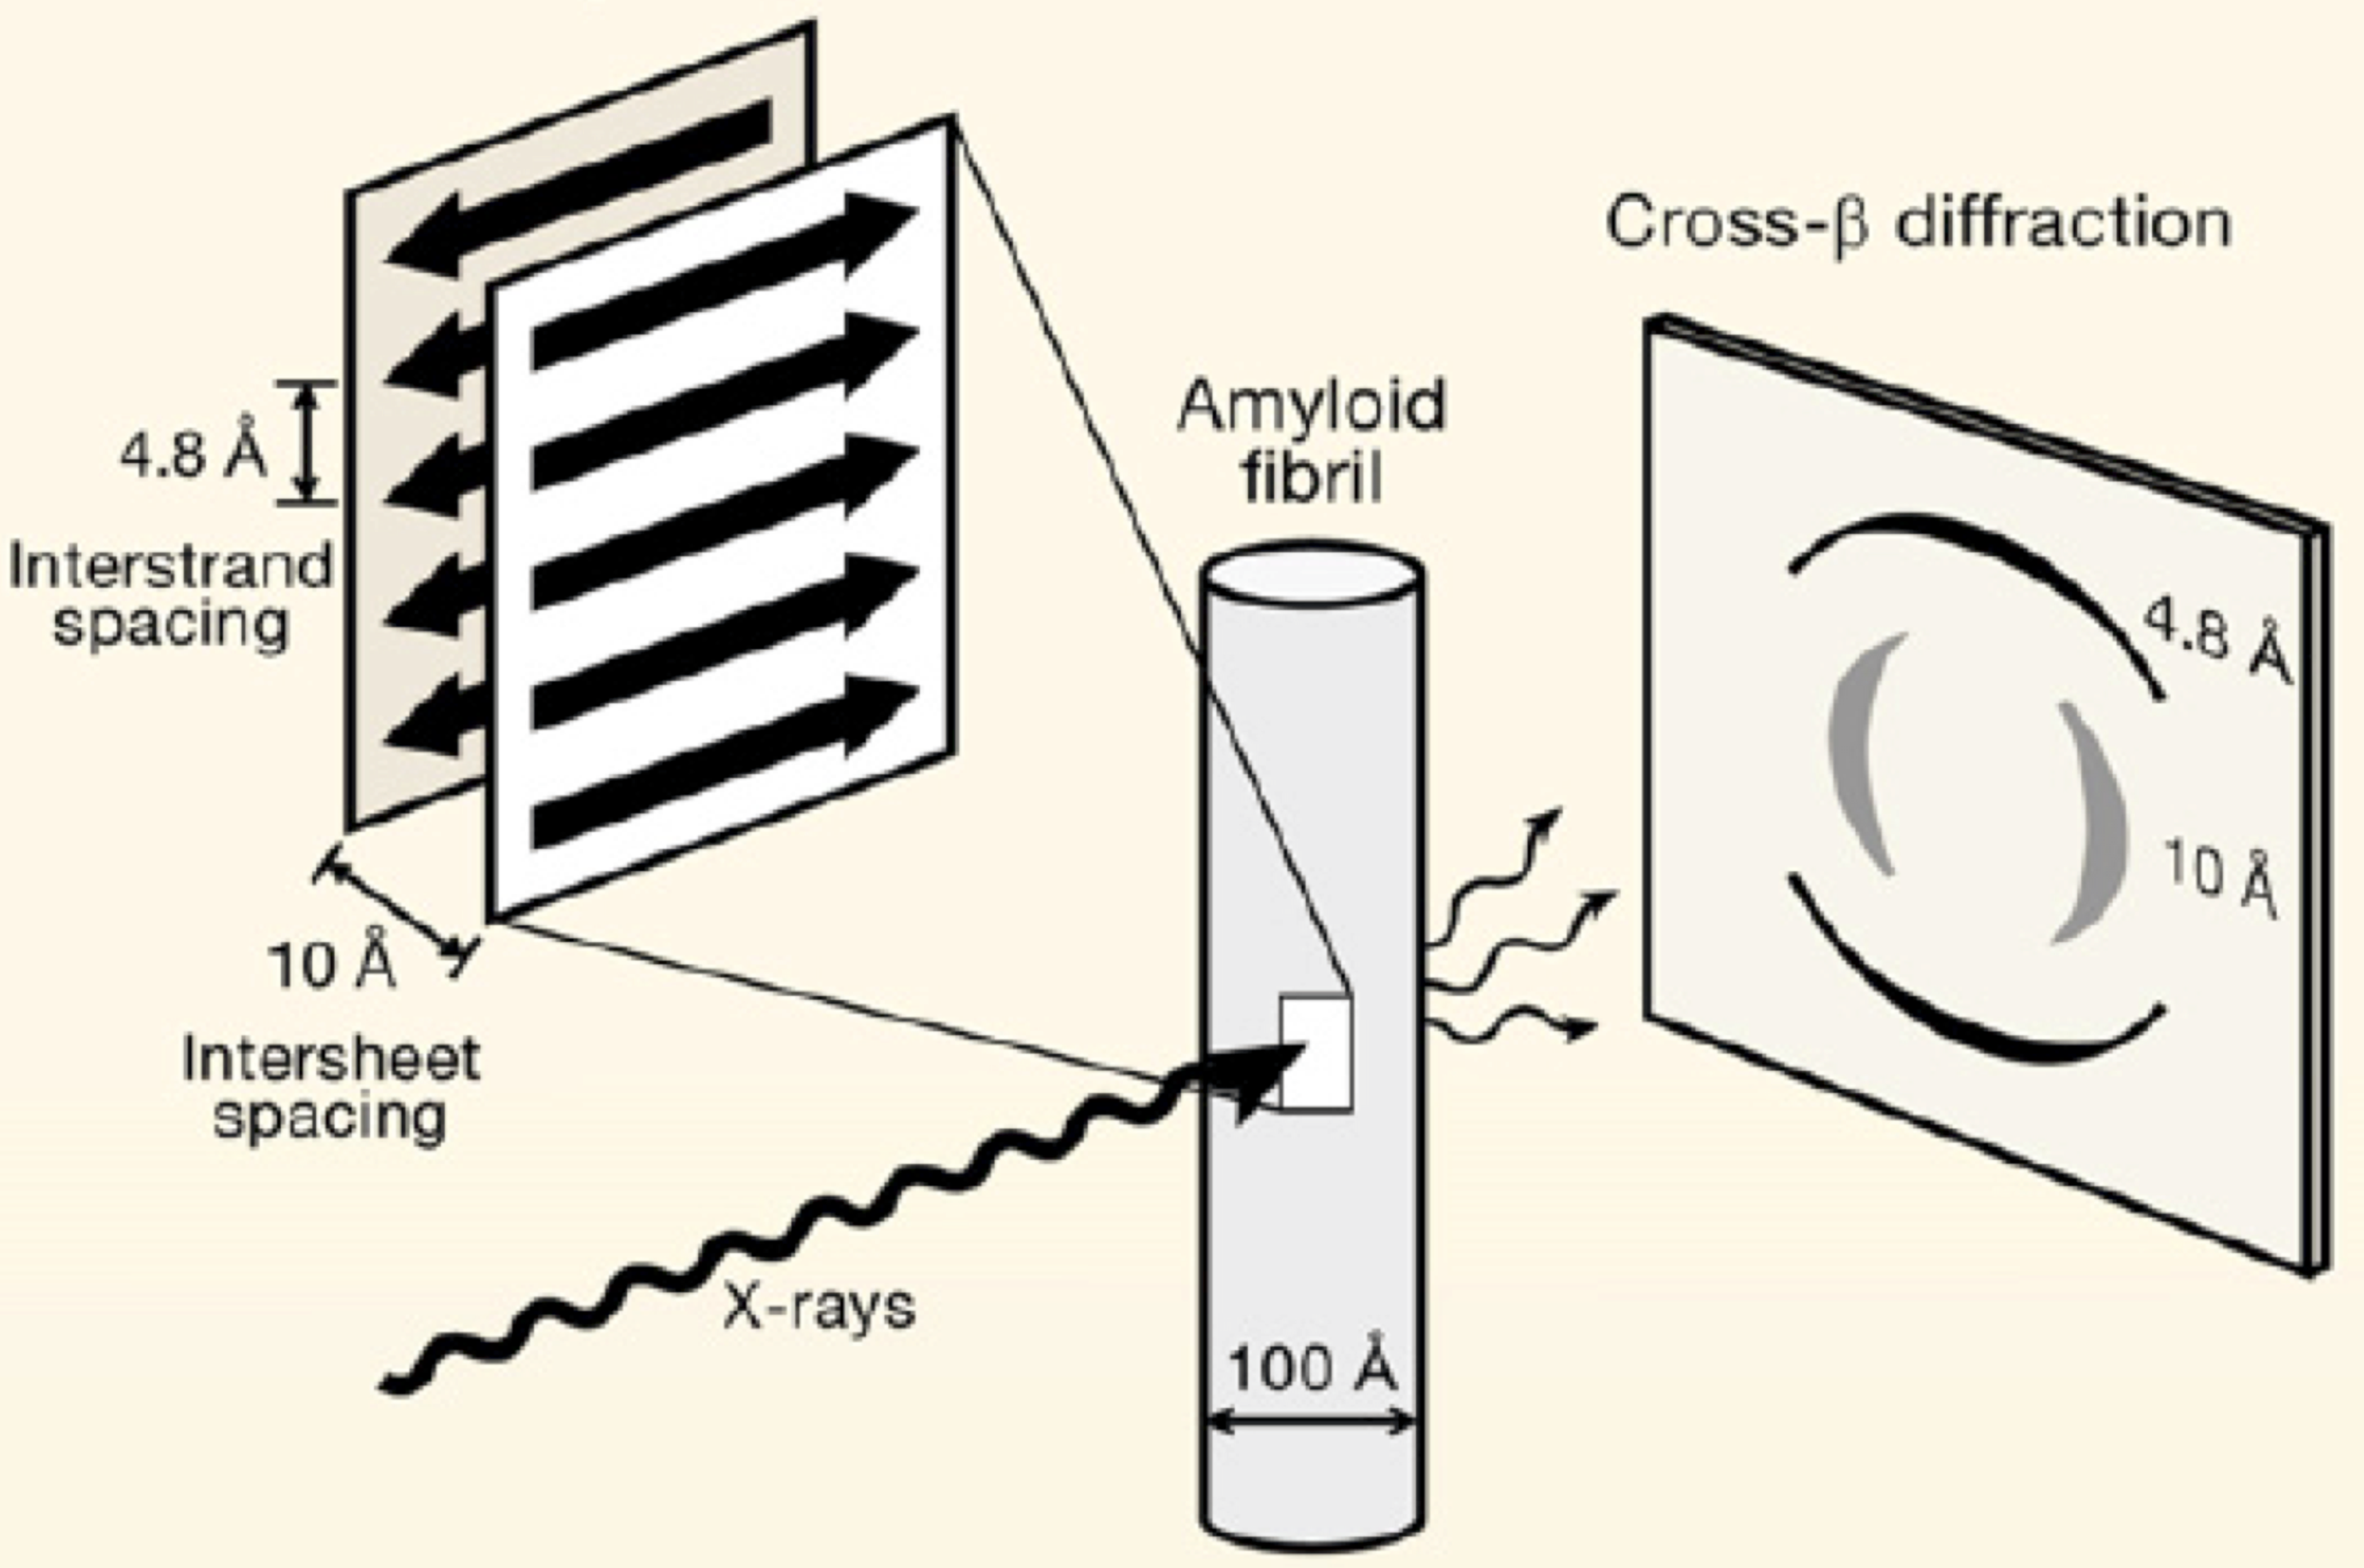
\includegraphics[width=6in]{figures/introduction/fibril_structure_diffraction.pdf}
  \caption[Characteristic cross-$\beta$ spacings from X-ray fibre diffraction studies of amyloid fibrils]{This is adapted from Eisenberg, 2012}
  \label{fig:fibril_diffraction}
\end{figure}

% Finding a treatment for AD and other fatal neurodegenerative diseases motivated many biochemical and biophysical studies of the amyloid state. 

Despite having dramatically different sequences, amyloid fibrils formed from different polypeptide all adopt a similar structure called the \crossbs.  The first structural studies of fibrils using X-ray fiber diffraction showed that a \crossb\ is characterized by a 4.8\angstrom\ interpeptide, and 10\angstrom\ intersheet spacing. XXX add more details to this description. XXX [Need to have a figure which shows this diffraction pattern, and EM data with cartoon model.] This defining characteristic of \crossb\ have now been adopted by biophysicists as an indication for the presence of amyloid fibrils.


Under the transmission electron microscope (TEM), fibrillar structures typical of many aggregates are visible as long, unbranched, often twisted ribbon-like structures nanometers in diameter (Figure~\ref{fig:fibril_TEM_SSNMR}). Independent measurements of fibrillar structure using different instruments have all confirmed the presence of \crossbs as the core structure of amyloid fibrils. (Figure~\ref{fig:fibril_diffraction})

% Other measurements 
% MPL Mass per unit length

Although \crossb\ is widely known, due to the insolubility and inherent non-crystalline nature of amyloid fibrils, the details of the fibril structure at the molecular level remained elusive until recently. Advances in solid-state NMR (SSNMR) and X-ray crystallography in the last decade have made major contributions to our knowledge of the molecular structure of amyloid fibrils.

\begin{figure}
  \centering
  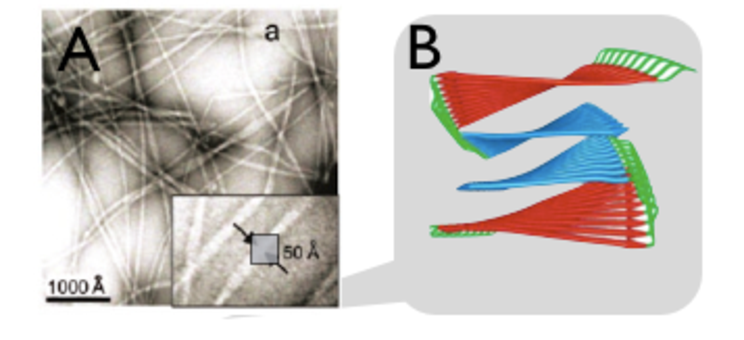
\includegraphics[width=6in]{figures/introduction/fibril_TEM_SSNMR.pdf}
  \caption[Characteristic cross-$\beta$ spacings from X-ray fibre diffraction studies of amyloid fibrils]{A Example EM images of oligomers.  Adapted from Bitan G. et al. 2003 and Walsh D. 1999 C TEM image of fibrils D SSNMR model proposed by Tycko et al.}
  \label{fig:fibril_TEM_SSNMR}
\end{figure}

% Describe the molecular structure of \abeta\ amyloid fibrils. 
% Briefly mention the techniques that can be used to obtain structural information of amyloid fibrils. 

% SSNMR
The initial molecular model of an amyloid fibril was for \abeta40, the peptide involved in Alzheimer's disease.  A SSNMR study on the amyloid fibrils of A$\beta$40 was done by Tycko et al in 2002. XXX The fibril core of \abeta40 involves the stretch sequence XXX-YYY. It is thought that residues A to B is disordered. The core fibril unit consists of a parallel in-register \bsheet, where each strand is a \bhairpin\ with peptide-peptide backbone hydrogen-bond along the long axis of the fibril. Figure~\ref{fig:fibril_TEM_SSNMR}


% X-ray structures
Furthermore, small peptide fragments that have characteristics of amyloid fibrils, which are also amenable to single crystal X-ray diffraction analysis have demonstrated similar type structures from those studied using SSNMR.  These structures obtained by X-ray crystallography have been described to have a dry interface with stacked sheets. (Figure~\ref{fig:fibril_xray_model})

\begin{figure}
  \centering
  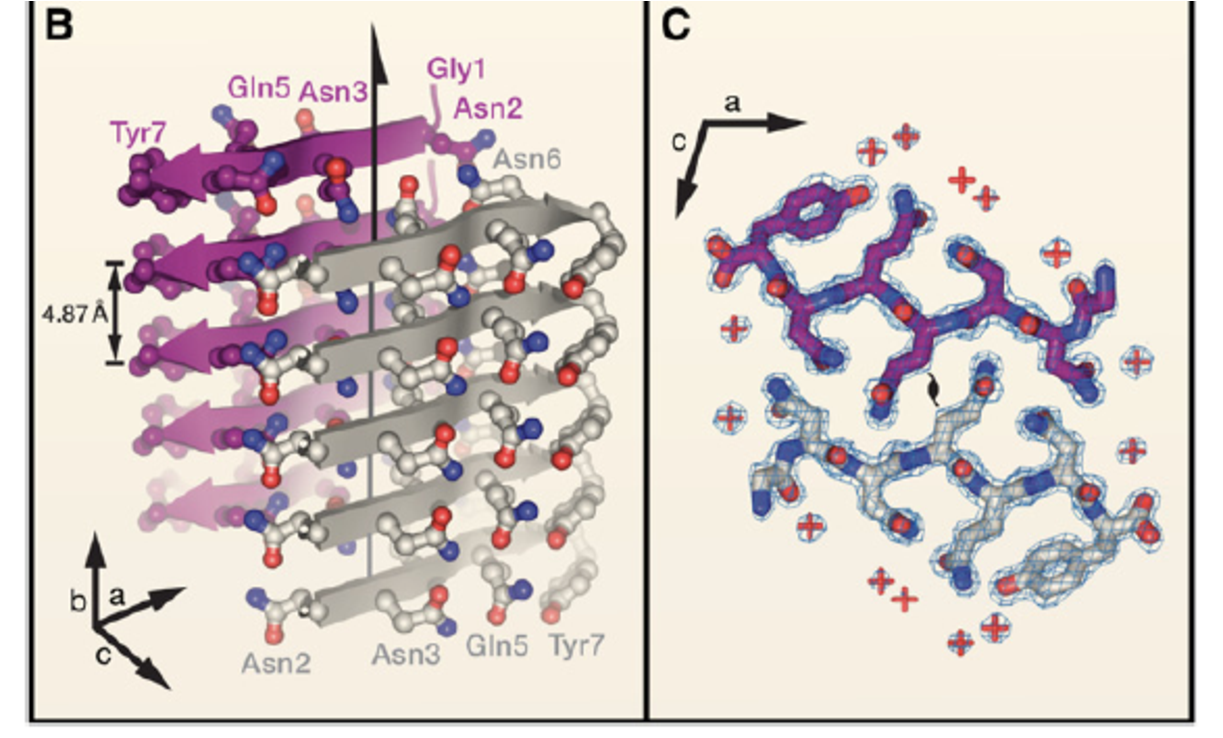
\includegraphics[width=6in]{figures/introduction/fibril_xray_model.pdf}
  \caption[Characteristic cross-$\beta$ spacings from X-ray fibre diffraction studies of amyloid fibrils]{This is adapted from Eisenberg, 2012}
  \label{fig:fibril_xray_model}
\end{figure}

% What do all fibrils have in common?
% Organization of the peptide backbone into beta-sheets; sheet stacking
The ubiquitous presence of a \crossbs supports that the organization of the peptidic backbone, common to all proteins, in to \bsheets\ is a major determinant of the fibrillar structure. Moreover, the proposed structures (some described above), indicate that the core region is composed of two to four sheets that interact closely with each other.

% I don't think I will talk about the twisting of the sheets too much.
% An interesting feature of these sheets is that they appear to be much less twisted than ex- pected from the analysis of the short arrays of β-strands that form β-sheets in globular protein structures. This feature was first proposed from cryo-EM and has been supported by Fourier transform infrared (FTIR) analy- ses (48, 61).

\subsection{Polymorphism of fibrils}

% Even fibrils formed from a single peptide can exhibit polymorphism .
Although all fibrils share the \crossbs, individual fibrils exhibit polymorphism at the molecular level which is dependent upon the experimental conditions under which they are formed.  % (Figure~\ref{fig:fibril_diffraction})
Fibrils may vary in the length of the beta-strand involved, side chain orientation. 

\subsection{Non-fibrillar oligomers}
\begin{figure}
  \centering
  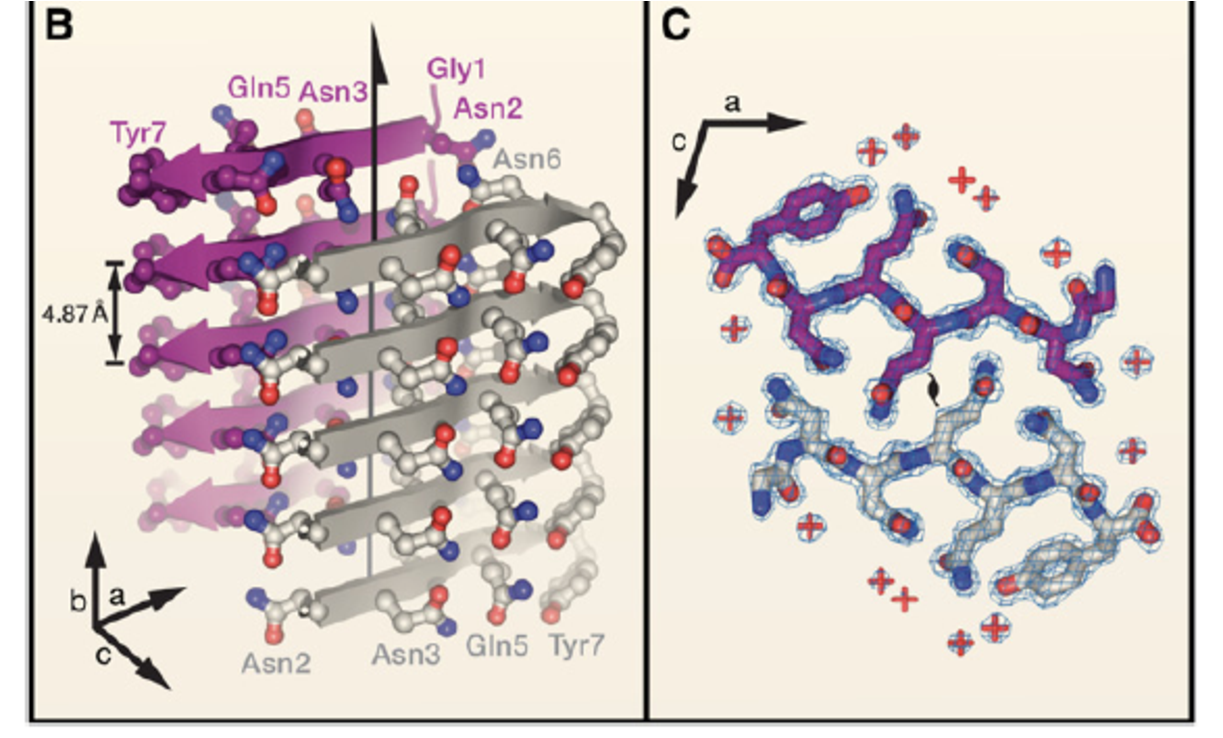
\includegraphics[width=6in]{figures/introduction/fibril_xray_model.pdf}
  \caption[Characteristic cross-$\beta$ spacings from X-ray fibre diffraction studies of amyloid fibrils]{This is adapted from Eisenberg, 2012}
  \label{fig:fibril_xray_model}
\end{figure}

Due to their structural disorder and their insolubility, molecular details of oligomers have been challenging to obtain using current structural determination techniques. 

EM and AFM experiments have shown that transient, unstable particles may appear prior to the formation of fibrils. In particular, soluble \abeta\ prefibrillar assemblies that are annular, spherical, or curvilinear in shape have been reported in literature.REF Protofibrils, in particular, are curvilinear, filamentous structures that are smaller than mature fibrils and are approximately 5-10 nm in diameter.9 Furthermore, protofibrils bind to dyes Thioflavin T (ThT) and Congo Red (CR), suggesting the presence of substantial β-sheet content.9, 13-15 Although some of these particles may be \bsheet-rich, they are morphologically distinct and are typically much smaller than fibrillar structures. Figure~\ref{fig:oligomers}

Despite the importance of these prefibrillar species in causing neurodegeneration, their molecular structures are still not known. However, a recent SSNMR study demonstrated that a late stage, neurotoxic Aβ40 spherical intermediate contained fibril-like β-sheet structure.16

[ Recent data show that non-fibrillar oligomers may contain fragments which are fibril-like in morphology. Most recently a study have shown that oligomers of \abeta\ ]
[ Should briefly read up on the book chapter by Pat Walsh]

\subsubsection{Amyloid Toxicity}
% I think outline some of the ideas / hypothesis about the link between amyloid and disease, but don't go into what people speculate or data on toxicity. It is related, but this is out of the scope of your thesis.

	% Key question in the field: What is the toxic species?
Multiple lines of research have identified oligomers as a likely causative agent for neuronal cell death. By contrast, the monomeric and fibril forms are thought to be less toxic than oligomers. It is hypothesized that soluble oligomers may cause toxicity by perturbing the integrity of cellular membranes through binding and disrupting the lipid bilayer (perhaps by making them ion permeable). \cite{Walsh:2007fu}

% Include a paragraph about amyloid formation and lipid membranes

% Understanding the toxicity or finding out whether there is a toxic species in part validates the amyloid hypothesis. 

% Here can lead into AD by saying well ... a widely known disease, where amyloid oligomers are thought to directly play a role in the disease process is AD.  

\section{Alzheimer's Disease}
One of the most well-known diseases involving amyloid formation is Alzheimer's Disease (AD), a devastating neurodegenerative disease that is most common cause of dementia in persons of age 65 or older.

% Pathological characterization
\begin{figure}
  \centering
  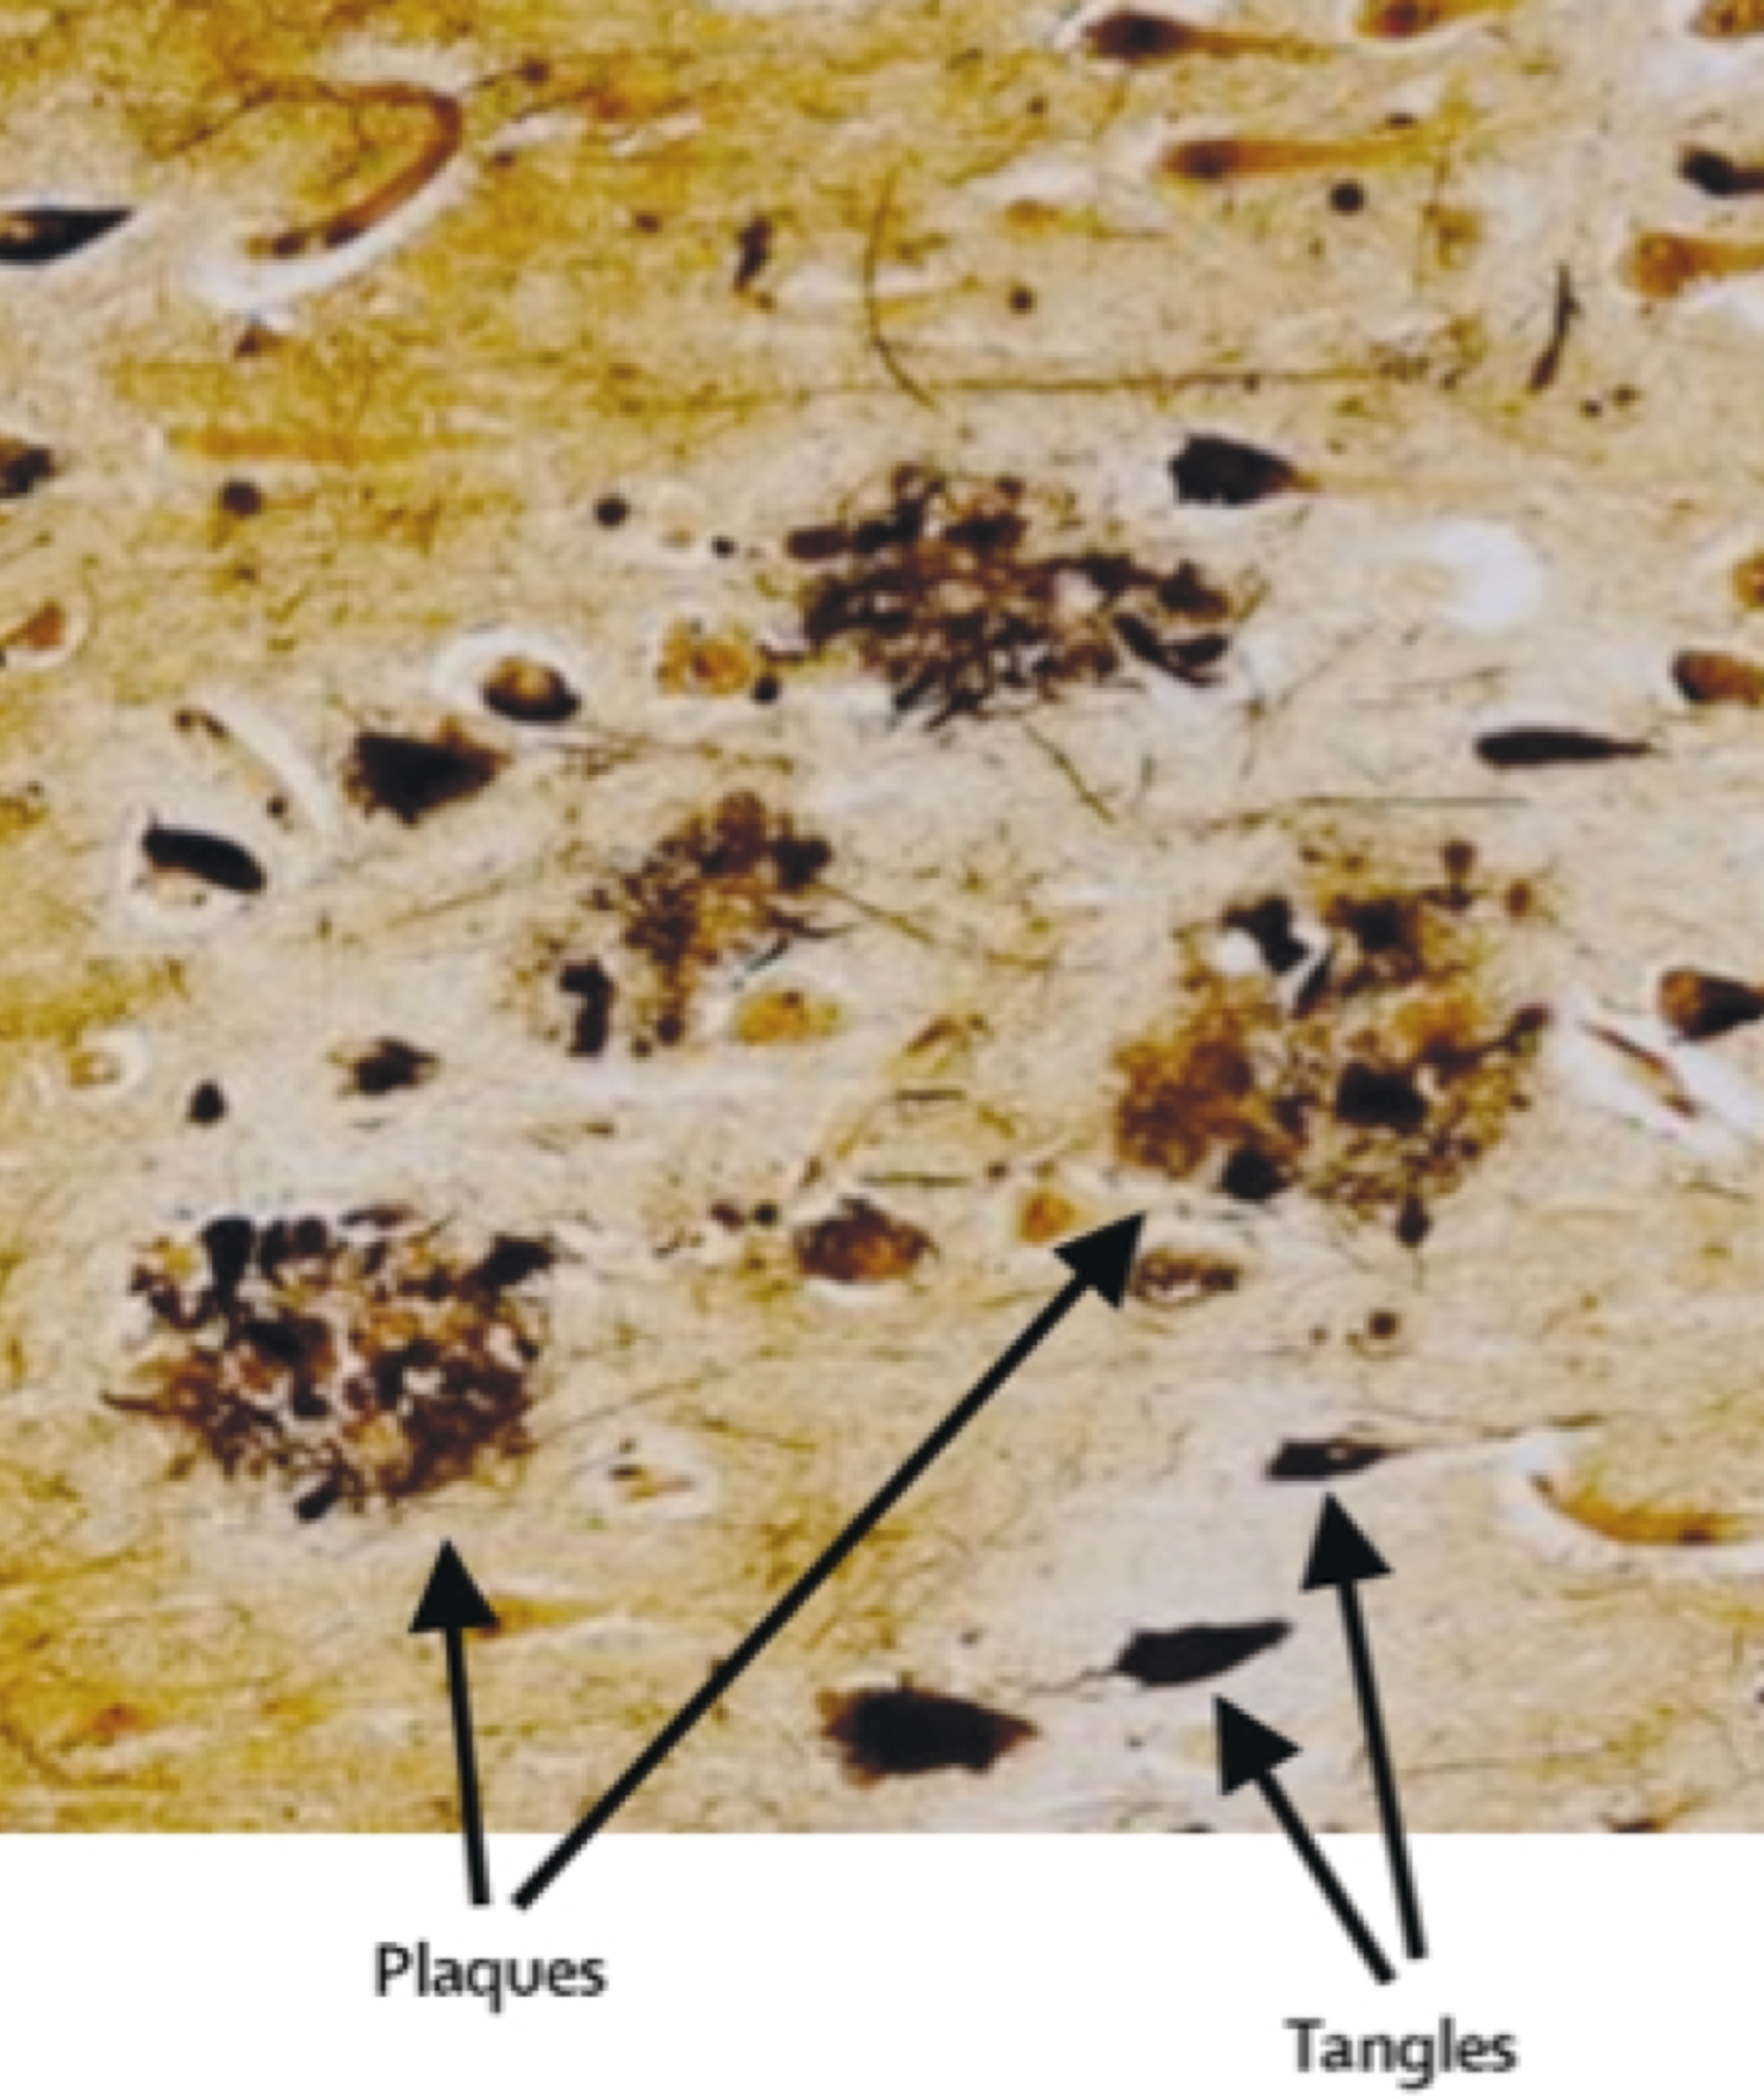
\includegraphics[width=6in]{figures/introduction/AD_tissue_pathology.pdf}
  \caption[Image of lesions formed by plaques and NFTs on brain tissue]{This is adapted from Blennow, 2006}
  \label{fig:AD_tissue_pathology}
\end{figure}

Upon examination, the brains of deceased AD patients show significant neuronal dystrophy.  Pathologically, AD is characterized by the presence of extracellular deposits of senile plaques and neurofibrillary tangles, which appear as lesions on stained neuronal tissue under light microscopy.(Figure~\ref{fig:AD_tissue_pathology})

Although it has been more than one hundred years since Dr. Alois Alzheimer first presented the association between the presence of neuronal plaques and the clinical symptoms of presenile dementia characteristic of Alzheimer's disease (AD), the exact relationship between the two is still under much contention.  It was not until in the 1980s, the protein \abeta\ was identified as the largest component of plaques. % How is Abeta produced ? Is it only involved in Abeta? What's the physiological role of Abeta?

The presence of amyloid plaque deposits in brains of deceased dementia patients led to the formulation of the long-standing amyloid hypothesis, which posits that amyloidogenesis of \abeta\ plays a key role in the initiation of AD. XXX

Although both plaques and NFTs appear together, many studies have indicated that NFTs plays a secondary role to \abeta\ in the pathogenesis of AD.
% More details on evidence which show that NFTs are not likely the causative species. Knock out mouse models ... mice do not develop AD, and instead develop tau pathologies  NFTs have also been shown to be affected by \abeta\ production.

% should I include more details on how Abeta is known to be produced in the body?
Monomeric \abeta\ is an approximately 4 kDa peptide produced by intramembrane proteolytic cleavage of the larger amyloid-$\beta$ precursor protein (APP) and is produced constitutively as part of the normal cellular metabolism.\{Selkoe, 2002 \#222\} APP is sequentially processed by the aspartyl proteases $\beta$-secretase and $\gamma$-secretase, where depending on the position of the cleavage by $\gamma$-secretase, a pool of \abeta peptides of lengths varying from 38 to 43 residues are produced. The peptides spanning residues 1-40 (\abetaforty) or 1-42 (\abetafortytwo) are predominantly found in AD-associated plaques. Neuritic plaques is composed of mainly \abetafortytwo, whereas \abetaforty\ is more commonly found in cerebralvascular plaques.

Multiple lines of evidence indicate that \abetafortytwo is likely to be the more deleterious form of \abeta. Genetic studies showed that mutations which cause early-onset AD also in turn increases the ratio of \abetafortytwo to \abetaforty.\cite{Hardy:1997tu} Moreover, in vitro, \abetafortytwo\ displays significantly higher propensity for aggregation than \abetaforty, despite differing by only two amino acids. In addition, \abetaforty\ and \abetafortytwo\ also have distinct aggregation pathways in vitro: \abetafortytwo is found to form a morphologically more diverse population of intermediate oligomers than \abetaforty.\cite{Bitan:2003ut}

% What about mice studies?

\abeta\ aggregates is present in a variety of morphologies in the brain. Although plaques are often visible in the dementia patients, the plaque load does not correlate with disease progression and severity, a puzzling aspect of AD.  Instead, synaptic loss correlated well with the concentration of soluble \abeta\ oligomers in the brain.

Currently there is a lack of treatment which targets the underlying disease. Most approved treatments today for AD only mitigates cognitive symptoms.  The vast number of structural and biochemical studies on amyloid structure have been crucial for the development of potential therapeutics for Alzheimer's disease.

%  Drug development for Alzheimer's has been on preventing amyloid aggregation and decreasing amyloid production. We will discuss this in more detail in later section XXX.
% Talk about how important it is to develop drugs for these amyloid disorders ... particularly for AD ... because it not only is a great economic burden on society, but a growing epidemic....

% \subsubsection{Other disorders}
% % Perhaps not enough to make it into its own subsection
% In addition to AD, other neurodegenerative diseases have been shown to involve the presence of amyloid.  Parkinson's disease, Huntington's, Prion disorders (Mad cow).  These diseases and their pathology are reviewed elsewhere and are beyond the scope of the thesis.
% I think I will not mention these things in detail in my introduction


\section{Amyloid Inhibition by small molecules: A promising method of treatment for AD}
% Cure, method of prevention; is there hope?

% In this section, I will provide an overview of some of the challenges to overcome when developing a small molecule therapeutic for Alzheimer's disease.  Furthermore, using this information, I will motivate why inositol is an exciting avenue to explore.

% Amyloid inhibition as a treatment for Alzheimer's disease and related amyloid disorders. 

% Briefly mention non-small molecule putative therapies which also acts via amyloid inhibition. The focus of this thesis will be on small-molecule amyloid inhibition.

% Use this as a transition into amyloid inhibition
% AD presents as a major economic and health burden to modern society.  With the longevity of our population, AD is approaching epidemic proportions with no cure or preventative therapy available.\cite{Blennow:2006wd}

Amyloids are attractive drug targets. Small molecules which targets amyloids may be an effective method of treatment for amyloid disorders because of the potential to treat the underlying disease. Through in vitro screening, many small molecules have been found to effect the amyloid aggregation pathway.  Some were demonstrated to inhibit amyloid fibrils, where as others were shown to arrest or reduce oligomer formation.
  
% Here I can take a cue from Justin Lemkul`'s recent review paper.
% Talk about the different kinds of small molecules that have been found to inhibition amyloid formation.  Here I will also provide a summary of what people know about the mechanism by which they inhibit amyloid formation.
Pharmacological perspective of the challenge of developing an Alzheimer's drug. In order to effectively treat Alzheimer's and other neurodegenerative diseases, small molecule drug candidates must pass the blood brain barrier at sufficient concentrations for inhibition.  This is difficult to achieve.
      
In vitro screening has led to the discovery of a large number of small-molecules which were found to affect the amyloid aggregation pathway. Many of these small molecules are thought to act by directly binding to amyloidogenic peptides and aggregates.

\begin{figure}
\centering
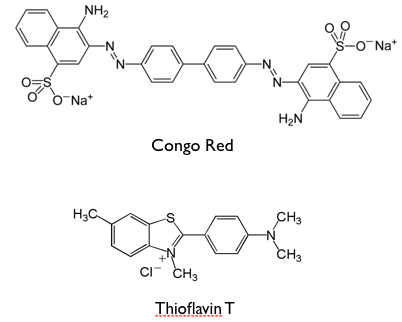
\includegraphics[width=3in]{figures/introduction/dyes.png}
\caption[Small molecule binders]{Amyloid binding dyes Congo Red and Thioflavin T}
\label{fig:amyloid_dyes}
\end{figure}

\subsection{Dye molecules}
Thioflavin T and Congo red are two dye molecules that are often used to identify the presence of amyloid fibrils.  

Early histological detection of amyloid binding was done using congo red, where upon binding fibrils exhibit red-green birefringence. Congo red requires the use of polarized light microscopy, a laborious process, and the interpretation of the birefringence is often not reproducible.

Thioflavin-T (ThT) is a benzathiole fluorescent dye also used to detect the presence of amyloid fibrils in post-mortem brain tissue samples, and monitor fibril formation in vitro. ThT exhibits a dramatic shift in the excitation spectrum maximum and an emission enhancement upon binding to fibrils, making it a sensitive and efficient report for the presence of amyloid fibrils.

Moreover, ThT is soluble in water and have \KD in the low \micromolar\ range.  ThT also binds uniformly across fibrils prepared from synthetic and biological sources.

The studies by Naiki et al. and LeVine showed that dye binding is linked to the presence of the \crossbs of fibrils, which led to the adoption of ThT dye binding as not only an indication of the presence of fibrils, but also as an indication of the presence of the \crossbs.

% Furthermore ThT fluorescence is only observed from those molecules that have bound to the fibrils.  
% ThT exhibits a shift in the excitation spectrum maximum, from 385 nm to 450 nm, and the emission maximum, from 445 nm to 482 nm

% This is from \cite{Wu:2011fd} which briefly summarizes why ThT binding gives rise to the excitation spectrum.
% These phenomena stem from two effects of binding.
% Firstly, steric and electronic stabilization (via charge trans- fer) of the ground-state charge distribution (7,8); and 2), restriction in the rotation of the aromatic rings of the dye (see Fig. 1 A) in its electronically excited state (9,10).



Both molecules appear to consistently bind mature amyloid fibrils.  Being \bsheet-rich does not imply that these dye molecules would bind. Also can affect fibril formation.(Fig.~\ref{fig:amyloid_dyes})

\begin{figure}
\centering
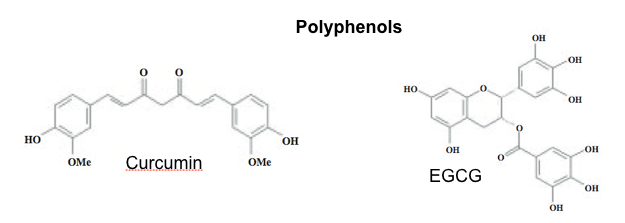
\includegraphics[width=6in]{figures/introduction/polyphenols.png}
\caption[Small molecule binders]{Polyphenols}
\label{fig:polyphenols}
\end{figure}

\subsection{Polyphenols}
Polyphenols,  is a large group of natural and synthetic molecules.  (−)-epigallocatechin-3-gallate, curcumin, and a polyphenolic grape seed extract, known for their anti-oxidant properties,  were recently discovered to be capable of affecting amyloid formation.(Fig.~\ref{fig:polyphenols})

\subsection{Inositol}
\begin{figure}
\centering
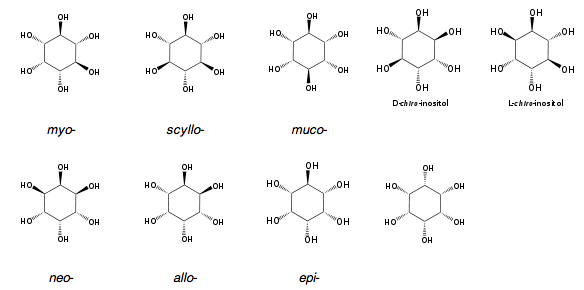
\includegraphics[width=6in]{figures/introduction/inositol.png}
\caption[Inositol]{Inositol stereoisomers}
\label{fig:inositols}
\end{figure}

% Should tell a little story of how inositol was discovered.  I remember that Chris Yip thought this might have been nice ... because it seems out of the blue to people.

% What I wrote in my transfer proposal:

Inositol with the molecular formula of \ce{C_6H_12O_6}, is a simple polyol with nine naturally occurring stereoisomers. Out of these nine isomers, seven are optically inactive, and the remaining two (L- and D-chiro-inositol) are chiral enantiomers.(Figure~\ref{fig:inositols})

% Here, use the physiological role of myo-inositol as a lead to transition into its role in amyloid inhibition.

Myo-inositol, the most abundant isomer, is ubiquitous in all eukaryotes and is a physiologically important osmolyte.  Furthermore, myo- is a precursor for inositol lipid synthesis: It is a constituent of phosphatidylinositol, an important phospholipid in membranes and second messenger systems. Once phosphorylated, myo-inositol phosphatides act as second messengers in intracellular signal transduction pathways.\cite{Fisher:2002tk}

Inositol is found in high concentrations in tissues of the human central nervous system (CNS): myo- And scyllo-inositol have approximate concentrations of 5 and 0.1-0.5 mM in the CNS, respectively.\cite{Fisher:2002tk} Accordingly, inositols also function as osmolytes in the CNS, where alterations in their concentrations are known to be associated with neuropathological conditions.\cite{Michaelis:1993gf, Fisher:2002tk}

% Role of inositol in amyloid inhibition. Here, include the background on how inositol was discovered as an \abeta\ amyloid fibril inhibitor
In recent years, scyllo-inositol have been identified as a promising therapeutic candidate for the treatment of Alzheimer's Disease.

Scyllo-, myo-, and epi-, but not chiro-inositol, have been shown to inhibit \abeta42 fibril assembly, stabilize an oligomeric complex of \abeta42, and attenuate \abeta-oligomer-induced neurotoxicity in vitro. Moreover, inositol exhibits stereochemistry-specific effects on \abeta\  fibril inhibition and cytotoxicity: scyllo- and epi- are more effective than myo-inositol, whereas chiro-inositol was inactive.\cite{McLaurin:2000bq}

An important therapeutic advantage of scyllo-inositol is its ability to readily crosses the bloodbrain barrier (BBB) (both actively and passively transported). Because it is not enzymatically broken down in the gut, it may be administered as a drug orally. 
% Inositol is synthesized inside the body ... or can be obtained via nutrition?  
		
In vivo studies with a transgenic mouse model of AD demonstrated that alleviation of symptoms after inositol treatment was correlated with a decrease in the levels of soluble \abeta\ oligomers, suggesting that the beneficial effects of scyllo-inositol may be attributed to the inhibition and/or disaggregation of high-order \abeta\ oligomers.\cite{McLaurin:2006eb}

Taken together, these results suggest that scyllo-inositol, and its derivatives, are a potential therapy for AD with the ability to change the course of the disease.\cite{Nitz:2008jl,Sun:2008ko}

% Include some data on human clinical trials (?) -- II was negative ... how to say it ? Should read phase II paper.
Presently scyllo-inositol completed both phase I and II of human clinical trials, where it was demonstrated that inositol is not toxic to healthy individuals at concentrations effective for amyloid inhibition.

\subsection{Commonalities between small molecule inhibitors}
% Commonalities between small molecules which appear to affect amyloid aggregation
Small molecule inhibitors share common chemical features and groups.  They are typically planar in geometry, have many aromatic rings, and polar functional groups (hydroxyl groups) around the edge of these aromatic rings.



\subsection{Molecular mechanisms of amyloid inhibition 
	            \\ by small molecules}
% Mechanism of action.
Some small molecules inhibit fibril formation, where as others may prevent oligomerization, but not fibrillation. A high concentration is often required to observe activity (micromolar to millimolar), which suggests that they may be non-specific inhibitors. EGCG, one such polyphenol, is known to have the lowest IC50.
    	% IC50 -- This quantitative measure indicates how much of a particular drug or other substance (inhibitor) is needed to inhibit a given biological process (or component of a process, i.e. an enzyme, cell, cell receptor or microorganism) by half.
      % EC50 -- The term half maximal effective concentration (EC50) refers to the concentration of a drug, antibody or toxicant which induces a response halfway between the baseline and maximum after some specified exposure time.[1] It is commonly used as a measure of drug's potency.
      % Ref: wikipedia
      
  	% Review of what is known about amyloid fibril ligand binding, specifically dyes.

Molecular mechanism of binding of dye molecules. Thought to bind flat on on the surface grooves of amyloid fibrils where they interact with hydrophobic groups exposed at the surface. 
      % Doesn't explain why the dye molecules are also able to suppress fibril formation.
      % Can the birefringence be explained by these binding modes? -- this is out of the scope of my thesis.  Don't put this in my thesis but I should be able to coherently explain this during my defense.

\section{Analogy to Sugar-protein binding}
% Does this section fit here? Where should I put it?
% Could use this as a prime example of protein-ligand interaction ...
% As a prime example of protein ligand interaction, one of the first systems that was used to understand binding was a sugar binding protein lysozyme ... -- No I think I will use early systems used to understand protein-ligand binding and if that was a sugar binding protein, then it will come off as a coincidence.
% This section is best discussed in the context of understanding inositol binding ...

% Mention some experimental techniques used to obtain protein sugar-binding modes, but the point here is not to review these methods ... but to point out that I am aware of these techniques.

\subsection{Sugar Binding modes}

% This section provides a nice lead in to the methods section
\section{Protein-ligand interactions}
\subsection{Forces involved in binding}
% Note that I may end up introducing the forces up in the earlier section -- reorganize as needed
\begin{outline}
	\1 Protein-ligand non-covalent interactions that are important for ligand binding and recognition
		\2 Electrostatic interactions. Polar (hydrogen bonding) and charge-charge interactions
		 % Here, it will benefit me to read Sarah's appendix C carefully.
		\2 Nonpolar (hydrophobic) interactions
		  \3 Van der Waals
\end{outline}

\subsection{Binding equilibria}
% subsection protein_ligand_binding_theory (end)
% Below is a summary of an excerpt from Tom's thesis on structure-based drug discovery.
% Design of antibiotics 
% 1) Target determination (biochemical)
% 2) Structural determination (Xray, NMR, or homology); active site identified; Here would be useful to get the holo structure of the protein
% 3) Screen for inhibitors against a chemical library or in silico docking.
\begin{outline}
	\1 Enzyme and its putative ligand typically bind specifically (high affinity binding).  We want to optimize binding specificity to increase the efficacy of the putative drug, and decrease adverse side effects (toxicity) in the human body.

	\1 The dissociation constant, $K_d$, is a measure of the affinity of a ligand for its binding site on the host protein. Pharmacologically, it can be interpreted as the concentration at which 50\% of the drug is bound to the protein. In experimental studies, $K_d$ is often used to quantitatively screen for potential drug candidates. 
  % A small $K_d$ suggests that the ligand may bind tightly to the protein.

	\1 Binding equilibrium

    \begin{equation}
      \left[ Protein\cdot Inositol \right] 
      \rightleftharpoons 
      \left[ Protein \right]+\left[ Inositol \right]
    \end{equation}
  
    % \2 Absolute binding free energy
    % \2 Relative binding free energy
    
	\1 The binding free energy of a ligand to a protein is directly related to its dissociation constant, $K_d$, the equilibrium constant of the above reaction

     \begin{equation}
        K_{d} = f_{ub}\frac{\left[ Protein \right]\left[ Inositol \right]}{\left[Protein \cdot Inositol\right]},
     \end{equation}
     
     % Add equation converting binding constant to gibbs free energies.
	\1 Experimental techniques for estimating $K_d$
		\2 What experimental techniques are used to estimate binding affinity? (May need to study up on this)
		\2 Isothermal titration calorimetry (ITC) is a technique which can be used to measure energetics of ligand binding to peptides.
\end{outline}

% \subsection{Role of chirality in drug binding}
% Stereoisomerism is important to the activity of molecules.  It modulates binding to proteins.
% Two types of stereochemistry
% Constitutional isomers - differs in bonding sequences and connectivity
% Stereoisomers - differs in orientation of their atoms in space, but no connectivity differences.
% Definition of chirality [Add schematic] ... etc
% Molecules with chirality have a non-superimposable mirror image, called an enantiomer.
% A carbon molecule with four different groups has chirality.

\section{Thesis objectives and rationale}
% Understanding amyloid inhibition in the context of the framework of traditional enzyme inhibition mechanism
\subsection{Challenges of amyloid inhibition}
\begin{outline}
       % However, most of these studies were focused on A$\beta$ and large A$\beta$ aggregates,\{Fawzi, 2008 \#553;Esposito, 2008 \#567;Sgourakis, 2007 \#609;Wei, 2006 \#656;Tarus, 2006 \#628 Karsai, 2006 \#658\} and thus, were computationally limited by the complexity of the molecular systems.

    \1 The protein-ligand binding model developed to understand enzyme inhibition cannot be directly applied to understand the molecular mechanism of amyloid inhibition by small molecules. 
    
      \2 Amyloid inhibitors are found to be very weak binders. How do non-specific inhibitors act as a drug? And how do we approach this with MD simulations?
      
      \2  Because the A$\beta$ amyloid aggregate pathway encompasses a variety of species, some of which has no folded structure, a single conformation cannot be assumed for binding. Furthermore, structural information of amyloidogenic species lags behind those of enzymes, which tends to be globular proteins amenable for X-ray crystallography. This means that the putative binding sites are not known.
      
      \2 The structural disorder of the peptides involved poses a challenge for obtaining converged properties from MD simulations. 
    
    	\1 A$\beta$ peptides are completely disordered.  We also do not know what the binding site looks like, where it is located on these structures.
    	
    \1 To date, few studies have attempted to provide statistically meaningful results pertaining to general mechanisms of protein self-aggregation and amyloid formation. Furthermore, despite the abundance of MD studies of A$\beta$, few studies have systematically examined the mechanism of action of small molecule inhibitors of amyloids

    \1 In AD, there is the added challenge of the drug being able to cross the brain barrier, while remaining non-neurotoxic.  What kind of drugs cross the BBB?  Typically hydrophobic drugs.
\end{outline}    

\subsection{Study Design and Rationale}
\begin{outline}
	\1 Here describe in detail how I designed my study to circumvent the challenges presented by the amyloid inhibition problem, and the limitations  of MD simulations. At this point, clearly explain and discuss my study design and rationale. (Fig.~\ref{fig:rationale})

  \begin{figure}
    \centering
    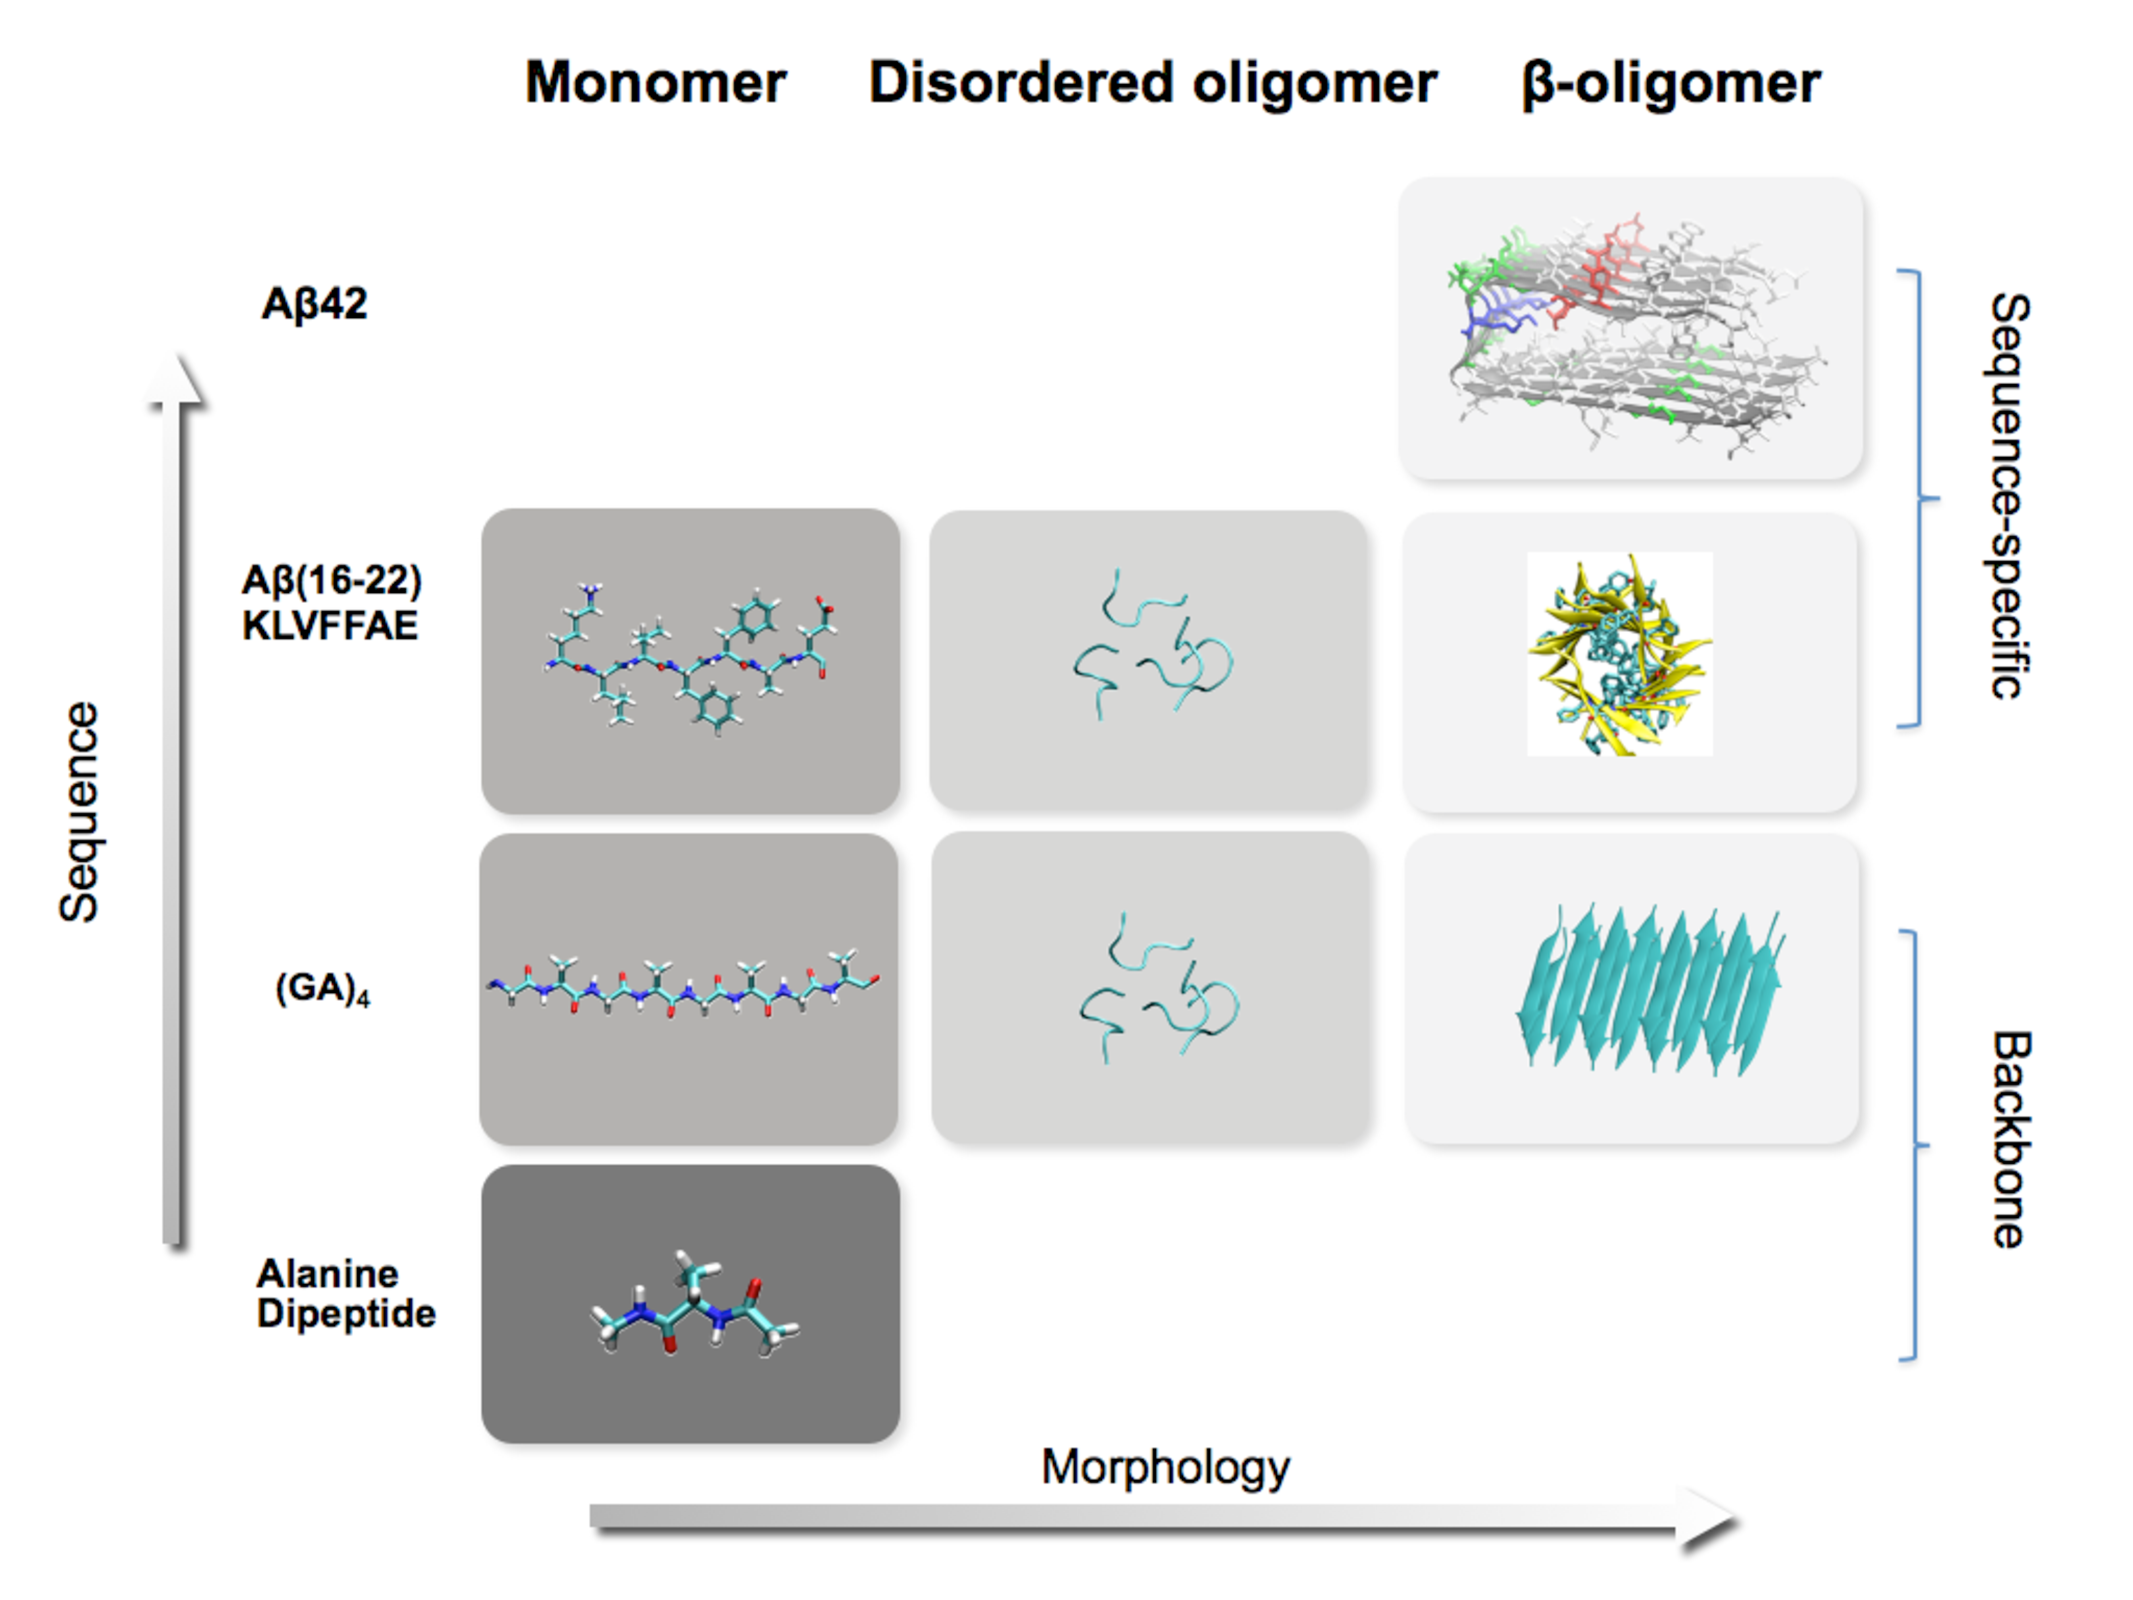
\includegraphics[width=6in]{figures/introduction/matrix.pdf}
    \caption[Rationale]{Shows the progression from small, model systems to larger and structurally more complex systems involving the full-length A$\beta$42 peptide.}
    \label{fig:rationale}
  \end{figure}

	\1 Beginning with the simplest model systems for an amyloidogenic peptide, the alanine dipeptide, we systematically examine binding of inositol with systems of both increasing sequence and structural complexity.

	% Use brute force simulations
	\1 We exploit conventional MD simulation techniques because simulation approaches used for understanding enzyme-ligand binding is not applicable. 
	
	\1 Instead, we use conventional MD simulations and repeats of independent simulations to determine the binding modes, and binding equilibria of inositol with amyloidogenic peptides and aggregates of A$\beta$.
\end{outline}

\section{Thesis Organization}
The first chapter introduces the thesis in the context of the field.  The second chapter introduces the main methods used in the work in the thesis. Chapters 3, 4, and 5 are the results of simulations of inositol with amyloid like peptides and aggregates. Chapter 6 shows work of the general applicability of our methods developed throughout this thesis to MD simulations to understand protein - carbohydrate binding. Chapter 7 provides discussion, suggestions for future work, and perspectives.

\addcontentsline{toc}{section}{Bibliography}
\bibliographystyle{plain}
\bibliography{chapter1}

% AD
% Treatment - harder to treat - lack of biochemical understanding of what causes disease, which makes it difficult to develop drugs for; lack of good diagnostic methods because treatment may not be effective at end stages of the disease where brain function won't e able to be rescued.
% Diagnosis - hard to diagnose
% AD is difficult to diagnose.  It is often not apparent that someone has AD until they exhibit symptoms severe enough to interfere with daily life or occupation. 

% Amyloid hypothesis - our best guess at what causes AD and provides the best guess at what we should be targeting. 
% Abeta Amyloid thus far provides the best clue to the molecular basis of AD, and thus a promising pathway to a cure for AD.

% In some individuals without dementia symptoms may have as much plaque as another with severe AD. Synaptic loss can be used as a measure of disease progression. 

% Perhaps use this as a transition into the general discussion of amyloid formation and structure -- not only specific to Abeta.
% Furthermore, amyloid have also been known to play beneficial roles in certain living systems. REF
% Increasing awareness of the amyloid state of proteins, and interest grew in amyloids because of their role in a variety of devastating human diseases.

% Fibrils

% In this section I will talk about how amyloid aggregation is thought to work. Introduce the thermodynamic model for understanding fibril formation.
%\chapter{Molecular Dynamics Simulations}
% Motivate MD simulations
\begin{outline}
\1 Molecular dynamics simulations are a useful tool to study the structure, dynamics, and interaction of biomolecules. MD simulations employ an empirical mathematical function to describe the atomic interactions in a molecular system, and together with classical laws of Newtonian mechanics, atomic trajectories of motion are generated. Thermodynamic and kinetic properties can then be extracted as time averages from these trajectories and used to make a number of predictions that are often experimentally challenging to observe or measure.

\1 MD simulation studies have been useful in studying many existing fundamental problems of biology and biochemistry, including protein dynamics and function, protein folding, biomolecular self-aggregation, and protein-ligand binding.
% Study protein dynamics - importance of protein dynamics.
\end{outline}

\section{Methodological Details} % (fold)
% Describe the details of molecular dynamics simulations

% A set of numerical computation algorithm which solves numerically solves the N-body problem. Solves a system of Newton's equations of motion, and provides the time-trajectory of atoms with femtosecond time resolution. 

% The integration algorithm is XXX. Time steps used are typically 2 femtoseconds to capture the hydrogen bond vibrational motion. [MORE DETAILS AND EQUATIONS HERE] [Ref: Chris Madill's and Tom's thesis]
% Details of the mathematics (need to review the basic theory + Taylor series expansion) - get a book - tomorrow maybe?

% The assumption at a hand-wave level adapted from Tom's thesis
\begin{outline}
	\1 Why is MD correct? Describe the fundamental assumptions of MD. Here, I want to give the readers who aren't familiar with the methodological details of MD a sense of the rigorousness of MD.
	
	\1 The Born-Oppenheimer approximation: electronic and nuclear motions are uncoupled, and therefore can be treated separately. 

	\1 MD does not account for the movement of electrons. Although electrons are not taken into account in MD simulations, their presence is implicitly accounted for via the use of potential energy functions.  Atomic nuclei can be treated as classical particles.

% \2 Review the basic derivations of MD simulation equations and why they work:
%   \3 Assume a small integration step (why is 2 fs chosen it is both biological and for numerical stability purposes). Roughly MD follows these steps:
%     \4 F = -grad E, where E is given by the force field potential energy function.
%     \4 Determine acceleration for each atom from the forces on each atom
%     \4 From acceleration determine momentum 
%     \4 Determine positions

% - Relationship between force and energy 
% - Relationship between momentum and velocity 
% - Why numerical approach must be used (no analytical solution for N > 2)
% - How is the force field plugged into the general algorithm.

  \1 Application of an empirical force field can be used approximate atomic interactions in the system. A force field typically has many parameters which need to be calculated. One approach to do this is to fit to quantum mechanical calculations.  Often experimentally observable quantities are computed for small compounds, and the fit is then adjusted by comparing to experimental measurements.
  
  \1 There many different force fields (AMBER, Gromos etc), each differing slightly in the potential energy function and parameterization. In this thesis we performed all of our simulations using the force field OPLS-AA/L.

  \1 Force field potential energy function
  % \[ V(R) = bonds + angles + impropers + dihedrals + pair interactions \]
  \begin{equation}
    \begin{split}
          E = \sum_{bonds} k_b(b-b_0)^2 
          + \sum_{angles} k_{\theta}(\theta - \theta_{0})^2 \\
          + \sum_{dihedrals} k_{\chi}(1 + cos(n\chi - \delta)) 
          + \sum_{impropers} k_{\gamma}(\phi - \phi_{0})^2 \\
          + \sum_{nonbonded} \frac{q_1q_2}{er} \\
          + \sum_{nonbonded} \epsilon [(\frac{r_{min}}{r})^{12} - 2(\frac{r_{min}}{r})^6]
    \end{split}    
  \end{equation}

% \1 Steps to produce a molecular simulation:
%   \2 First take a structure from crystallography or NMR, or homology-modelling data.
%   \2 In the algorithm, the forces acting on each atom are estimated from [insert equation here]
\end{outline}

\section{Challenges and limitations of MD simulations}
\begin{outline}
	\1 MD is computationally challenging because of limitations in length and time scales.
	
		\2 Length scale. Large systems are too complex to obtain statistics and quantitative predictions.
			
		% Evaluating the convergence of simulations is still a challenge
		\2 Time scale. Relevant biochemical reactions such as protein folding happens on the time scale of milliseconds, hours, and days. Currently with MD simulations, we are routinely able to approach the microsecond time scale, massive computing power is still insufficient to observe phenomena on the millisecond timescale. % Ref: DE Shaw Research.
		\2 Obtaining convergence. Explain why this is difficult, in particular for systems with disordered peptides.
	\1 Limitations in the accuracy of current force fields.
\end{outline}		

\section{Application of MD: structure-based drug discovery}
\begin{outline}
% \1 (Why computational?) Can help us get protein dynamics is important for understanding protein function. We want to understand protein function because we want to be able to design drugs to cure diseases.

% \1 A important application of MD simulation in biochemistry is the predicting of protein-ligand binding free energies.

	\1 Cheaper, faster, get atomic resolution. Modeling can be used to rapidly prototype an experimental idea -- for example, one can performed computer alchemy, that is, ''mutate``'' residues to test hypothesis. In recent years structure-based computer modeling of protein-ligand interactions have become a core component of modern drug discovery. REF: Mobley, Dill 2004 Computers are advancing thus it is cheaper, MD may be used as a drug discovery platform. In terms of drug discovery, can be used to determine whether a chemical change will produce a more potent drug candidate.

	% MD is more straightforward if there is a folded, protein structure.
	\1 A broad application of simulations of proteins is to computationally design drugs and combining that with structure-based drug design.
	
	  \2 First you solve a protein structure using conventional structural determination methods such as X-ray crystallography or perhaps NMR.  Typically you would have an idea of where the binding pocket is as well. 
	
	  \2 Then taking a protein force field and apply MD simulations to the protein structure in the presence of the putative ligand.  Because the binding affinity is very high (usually the binding specificity ...
	% The sentences above are pretty repetitive. Combine and tighten.

	\1 Typically, an X-ray crystal structure of a target is first determined with a putative binding site. [See Tom's thesis]
	
	\1 Ligands which may act as potential drugs typically have high binding affinity to the binding site. The goal is to find high specificity inhibitor of a protein (usually an enzyme). The binding free energy is an important quantity which can be used to evaluate how well a ligand binds. One method of estimating binding affinity is by using computational docking methods, where the binding affinity is measured without taking into account of the protein conformational entropy.  Although docking is computationally less expensive, it is inaccurate for identifying true drug candidates because binding often involves changes in protein conformation.

	\1 Currently state of the art computational binding studies take into the account of change in protein conformation. MD simulations is an effective method, where the protein and drug is allowed to relax and freely move about in the system.

	\1 However, in the case of very specific binding, observing binding events is a low probability event in MD simulations. Therefore it is not practical to use brute-force MD sampling to determine free energies.

	  \2 Methods used to determine binding free energies using MD:
	  % \3 Linear interaction energy -- Out of scope
	  % \3 MM/PBSA - no explicit account for solvents -- Out of scope
	  	\3 Thermodynamic perturbation \cite{Gilson:2007hz}
			\4 thermodynamic integration
			\4 free energy perturbation
\end{outline}

\section{Review of MD studies of amyloid inhibition by small molecules}
MD studies using brute-force sampling. Aid in medicinal chemistry by making suggestions for how to design new AD drugs

\begin{outline}
	%  Excerpt from Transfer proposal
	\1 In recent years, molecular dynamics simulations have been intensively used to investigate the molecular basis of the structure and stability of amyloid fibrils. However, most of these studies were focused on A$\beta$ and large A$\beta$ aggregates,\{Fawzi, 2008 \#553;Esposito, 2008 \#567;Sgourakis, 2007 \#609;Wei, 2006 \#656;Tarus, 2006 \#628 Karsai, 2006 \#658\} and thus, were computationally limited by the complexity of the molecular systems. To date, few studies have attempted to provide statistically meaningful results pertaining to general mechanisms of protein self-aggregation and amyloid formation. Furthermore, despite the abundance of MD studies of A$\beta$, few studies have systematically examined the mechanism of action of small molecule inhibitors of amyloids. MD simulations of Congo red binding have only been done with the protofibril-like crystal structure composed of the segment GNNQQNY.\{Wu, 2007 \#621\} A recent simulation study of an N-methylated peptide with A$\beta$16-22 models of amyloid aggregates has provided insight into the possible mechanism of action of peptide inhibitors of amyloid formation.\{Soto, 2007 \#597\} This peptide inhibitor was shown to preferentially bind monomers to form dimers, possibly acting to inhibit fibril formation by sequestering monomers. However, peptide-based inhibitors have poor pharmacological profiles as they are actively broken down by proteases in the stomach and are difficult to transport across the blood-brain barrier. In addition, these peptide inhibitors specifically target A$\beta$ and thus do not have the potential to treat multiple amyloid diseases.
\end{outline}

\section{Molecular mechanism of binding of dye molecules}
% Review of what is known about dye binding on amyloid fibrils.
Two types of binding modes. Bind flat on amyloid surface. Interact with hydrophobic groups exposed on the amyloid fibrils.
Doesn't explain why the dye molecules are also able to suppress fibril formation.

% Can the birefringence be explained by these binding modes? -- this is out of the scope of my thesis


\section{Thesis objectives and rationale}
% Understanding amyloid inhibition in the context of the framework of traditional enzyme inhibition mechanism
\subsection{Differences between amyloid inhibition and enzyme inhibition}
\begin{outline}
    \1 Can we think about amyloid inhibition as a tradition enzyme inhibition problem ? Not exactly. We have the exact opposite of this framework with amyloids. Most inhibitors are found to be very weak binders ... how are they working as a drug then? And how do we approach this with MD simulations?

    \1 The enzyme and ligand inhibition / binding model cannot be directly applied to understanding amyloid inhibition.  No folded structure, no putative structure (there are many, which one?), no putative binding site (generally presents a surface).

    \1 In AD, there is the added challenge of the drug being able to cross the brain barrier, while remaining non-neurotoxic.  What kind of drugs cross the BBB?  Typically hydrophobic drugs.
\end{outline}    

\subsection{Study Design and Rationale}
\begin{outline}
	\1 Here describe how I designed my study to navigate the challenges presented by the amyloid inhibition problem and MD simulations - rationale. At this point, explain and discuss my approach, study-design and rationale. Include the matrix figure.

	% \begin{figure}
	%   \centering
	%   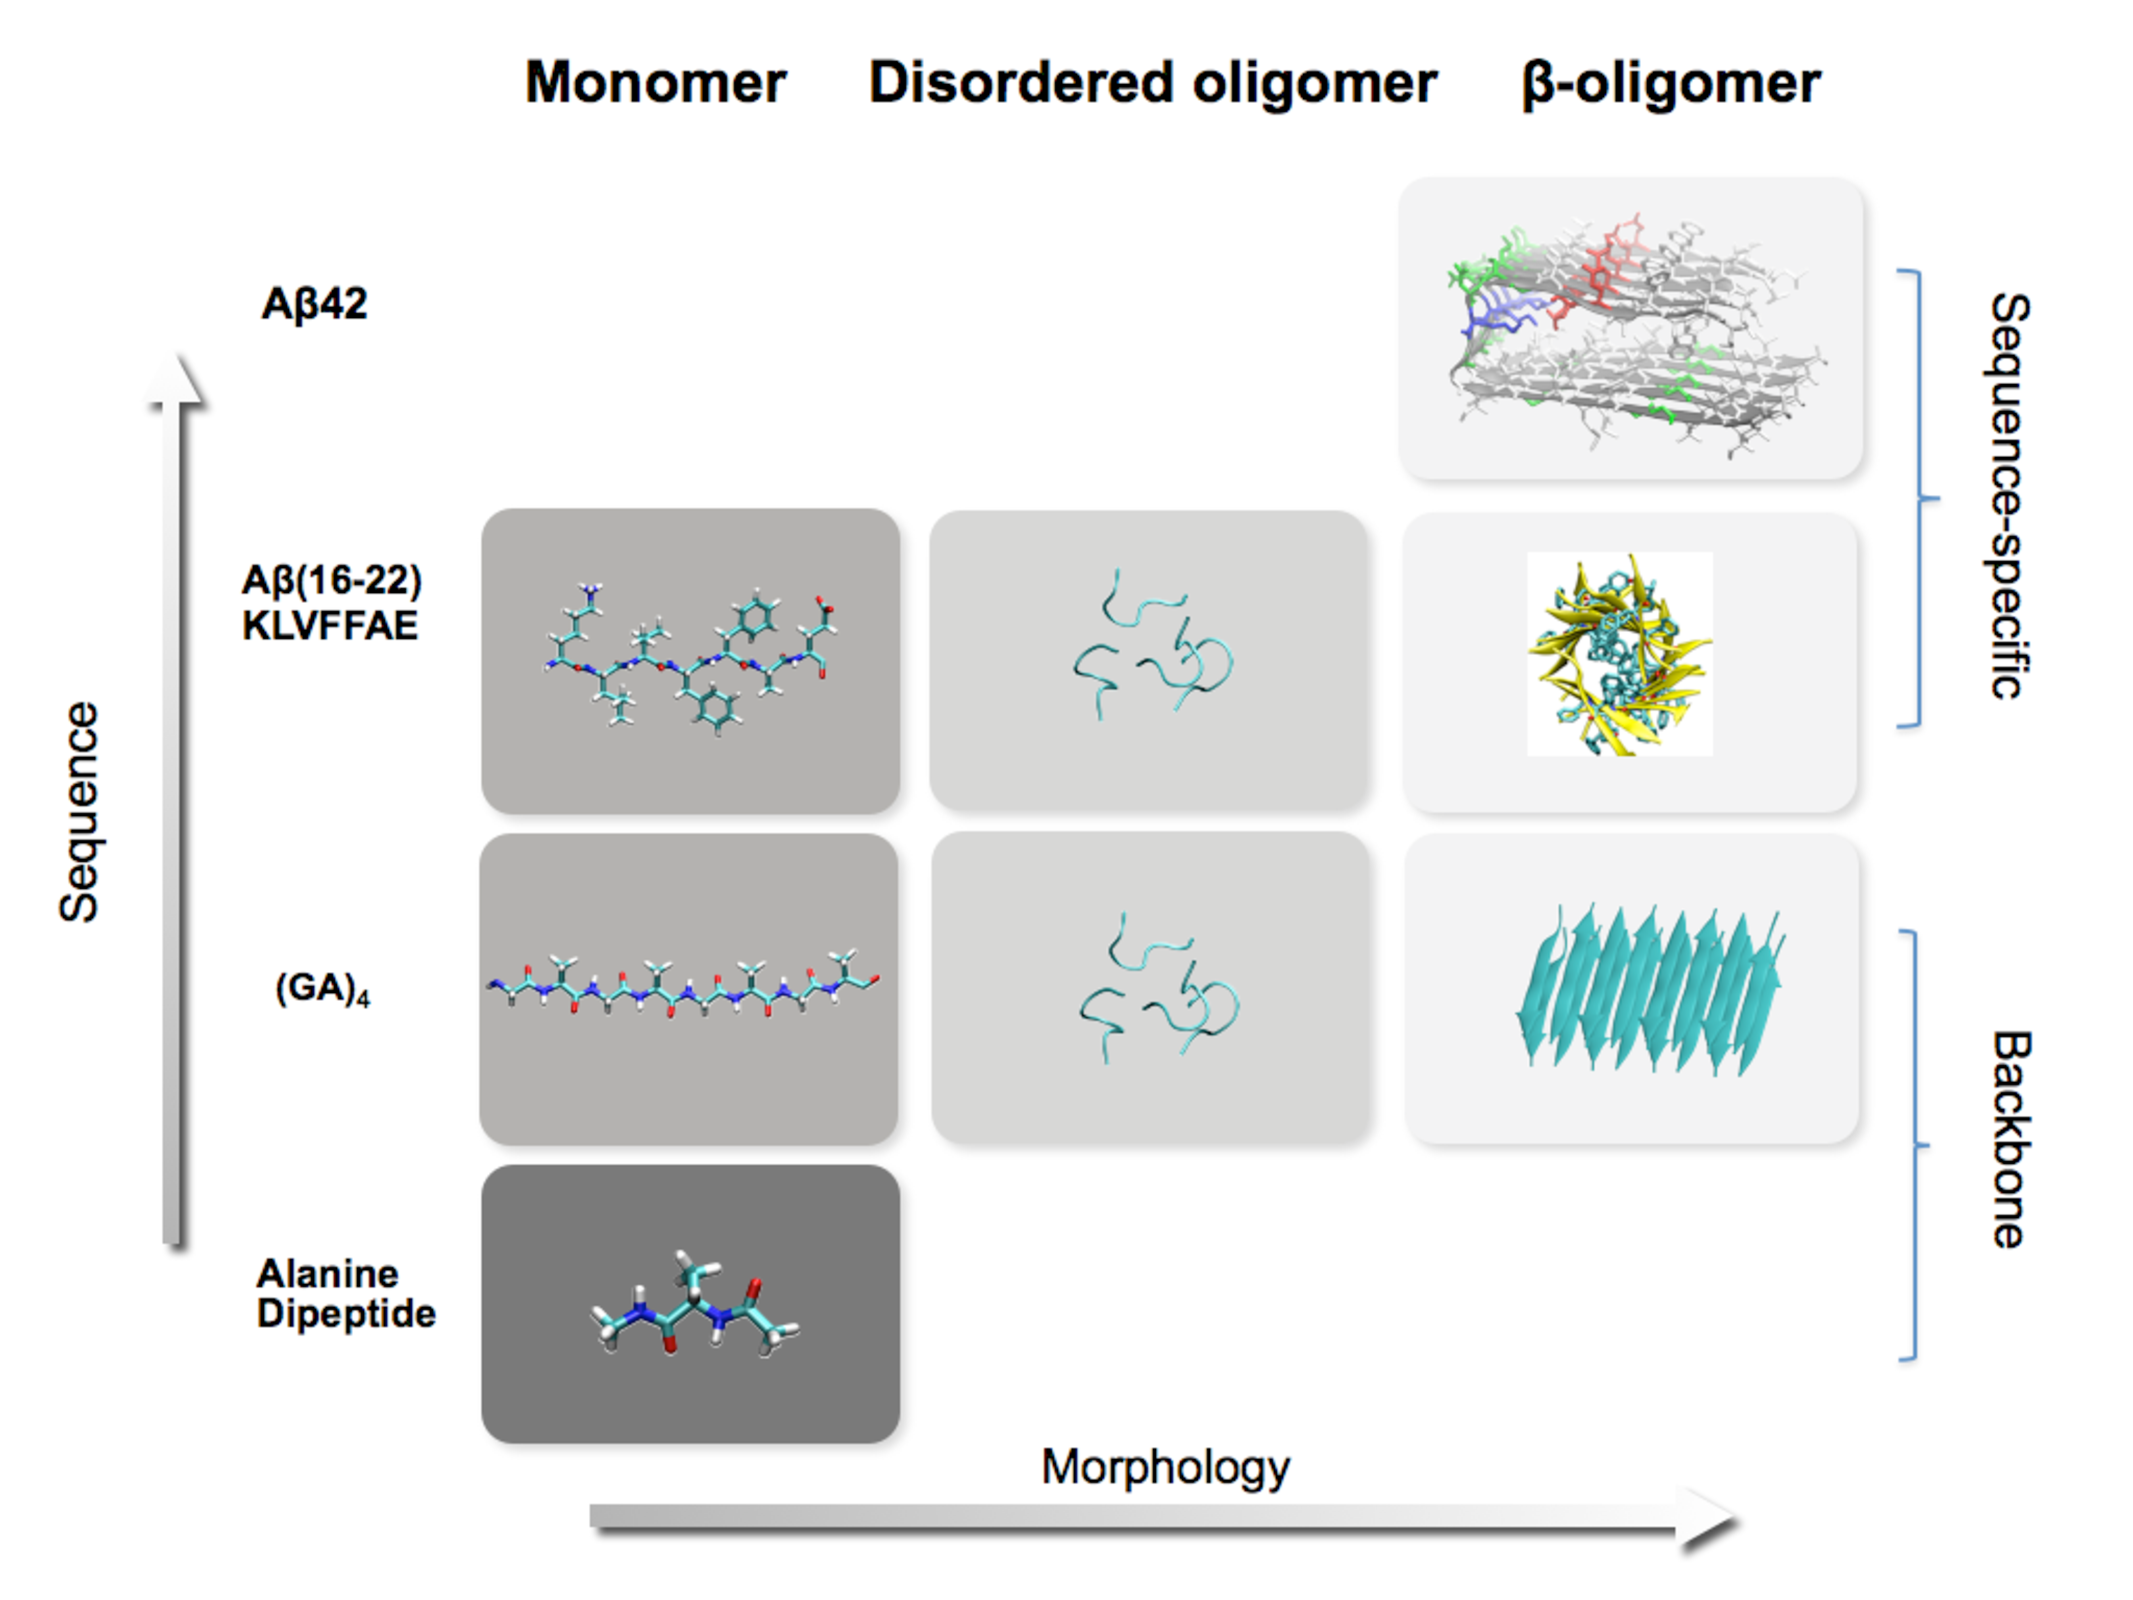
\includegraphics[width=6in]{figures/introduction/matrix.pdf}
	%   \caption[Rationale]{Shows the progression from small, model systems to larger and structurally more complex systems involving the full-length A$\beta$42 peptide.}
	%   \label{fig:rationale}
	% \end{figure}

	\1 A$\beta$ peptides are completely disordered.  Because A$\beta$ amyloid formation consists of many different types of aggregates, a single conformation cannot be assumed for binding.  We also do not know what the binding site looks like, where it is located on these structures.

	\1 Beginning with the simplest model systems for an amyloidogenic peptide, the alanine dipeptide, we systematically examine binding of inositol with systems of both increasing sequence and structural complexity.

	% Use brute force simulations
	\1 We exploit conventional MD simulation techniques because we can't readily pick a reaction coordinate as in tradition enzyme-ligand binding problems. Using large-scale sampling and repeats of many simulations to determine the binding mechanism and binding equilibria.	
\end{outline}

\addcontentsline{toc}{section}{Bibliography}
\bibliographystyle{plain}
\bibliography{chapter2}

% Model peptides
% % Chapter cover page
\chapter{Binding of inositol stereoisomers to model amyloidogenic peptides}

The contents of this section were adapted from an article published in the \emph{Journal of Physical Chemistry}.
\\
\\
\emph{Reference}:
Li, G., Rauscher, S., Baud, S., & Pomès, R. (2012). Binding of Inositol Stereoisomers To Model Amyloidogenic Peptides. Journal of Physical Chemistry B, 116(3), 1111–1119.
\\
\\
\emph{Contributions}:
Grace Li conducted the research and wrote the section. Régis Pomès provided editorial input and guidance.

\newpage

\section{Summary}
The self-aggregation of proteins into amyloid fibrils is a pathological hallmark of numerous incurable diseases such as Alzheimer's disease. Scyllo-inositol is a stereochemistry-dependent in vitro inhibitor of amyloid formation. As the first step to elucidate its mechanism of action, we present molecular dynamics simulations of scyllo-inositol and its inactive stereoisomer, chiro-inositol, with simple peptide models, alanine dipeptide (ADP) and $(Gly-Ala)_4$. We characterize molecular interactions and compute equilibrium binding constants between inositol and ADP as well as, successively, monomers, amorphous aggregates, and fibril-like \bsheet\ aggregates of $(Gly-Ala)_4$.\cite{Balbach:2000p49}
Inositol interacts weakly with all peptide systems considered, with mM to M affinities, and displaces the conformational equilibria of ADP but not of the $(Gly-Ala)_4$ systems. However, scyllo- and chiro-inositol adopt different binding modes on the surface of \bsheet\ aggregates. These results suggest that inositol does not inhibit amyloid formation by breaking up preformed aggregates, but rather by binding to the surface of pre-fibrillar aggregates.

\section{Introduction}
Amyloid fibrils formed by various peptides and proteins are known to be associated with neurodegenerative diseases, type II diabetes, and prion-related disorders.\cite{Chiti:2006p20} In particular, amyloid fibrils of \abeta\ peptides are found in the extracellular deposits of neuronal plaques and are thought to be central to the pathogenesis of Alzheimer’s Disease (AD),\cite{Chiti:2006p20,Hardy:2002p27} a common and incurable neurodegenerative disease causing dementia and eventual death. 

In recent years, amyloid fibril formation was discovered to be a common phenomenon among many proteins in vitro; that is, under certain misfolding and denaturing conditions, proteins can self-aggregate to form amyloid fibrils.\cite{Chiti:2006p20} When viewed with negatively-stained transmission electron microscopy, amyloid fibrils appear as elongated, rope-like structures that are often 100 nm in length.\cite{Chiti:2006p20} The core structure of all amyloid fibrils is the cross-β sheet.\cite{Chiti:2006p20,Serpell:2000p39} At the molecular level, NMR\cite{Balbach:2000p49,Petkova:2006p48} and X-ray crystallography\cite{Sawaya:2007p11} studies have revealed that the cross-β structure is comprised of extended polypeptides organized in highly-ordered, in-register \bsheets. Although amyloid fibrils are a pathological hallmark of amyloid-based diseases, smaller nonfibrillar oligomers as little as three or four peptides in size have been demonstrated to display higher cytoxicity than mature fibrils.\cite{Gong:2003p22,Bitan:2003p10,Caughey:2009p5,Keshet:2010p61,Kitamura:2010p6,Lambert:1998p60,Selkoe:2008p16}

An important strategy to finding a cure to AD and other amyloid diseases is to derive new therapeutic candidates through the rational design of effective small-molecule inhibitors of amyloid formation. In recent years, a number of small molecules capable of preventing aggregation and/or fibril formation have been discovered and have emerged as potential therapeutic approaches for protein misfolding diseases.\cite{Frid:2007p65,Hawkes:2009p9,LeVine:2009p38,Necula:2007p42,ScherzerAttali:2010p63,Sood:2009p14} Interestingly, many of these small molecules share common chemical structural features, such as aromaticity and the presence of multiple hydrogen-bonding groups.\cite{Ehrnhoefer:2008p8,Liu:2009p18,Liu:2005p7,Porat:2006p33} However, the molecular basis of the structure-activity relationship of these small molecules is not understood, thus hindering drug development efforts for amyloid-based diseases. 
Recently, one such small molecule, scyllo-inositol, has shown promise as a therapeutic for AD.\cite{McLaurin:2006p29,McLaurin:2000p64} Scyllo-inositol is one of nine stereoisomers that belongs to a class of cyclic polyols called cyclohexanehexols. Four stereoisomers, myo-, epi-, scyllo- and chiro-inositol (Figure~\ref{fig:inositol}) are physiologically active.\cite{Fisher:2002p62} Myo-inositol, the most abundant stereoisomer, plays an important role in signal transduction as precursor of phospholipid headgroups: once phosphorylated, myo-inositol phosphatides act as second messengers in intracellular signal transduction pathways.\cite{Fisher:2002p62} Importantly for its therapeutic potential, inositol readily crosses the blood-brain barrier. Myo- and scyllo-inositol are found in tissues of the human central nervous system (CNS), with approximate concentrations of 5 mM and 0.1 to 0.5 mM, respectively.\cite{Michaelis:1993p89} Accordingly, they are also important osmolytes in the CNS, where alterations in their concentration have been associated with neuropathological conditions.\cite{Fisher:2002p62,Michell:2008p4}
 
\begin{figure}[hb]
  \centering
  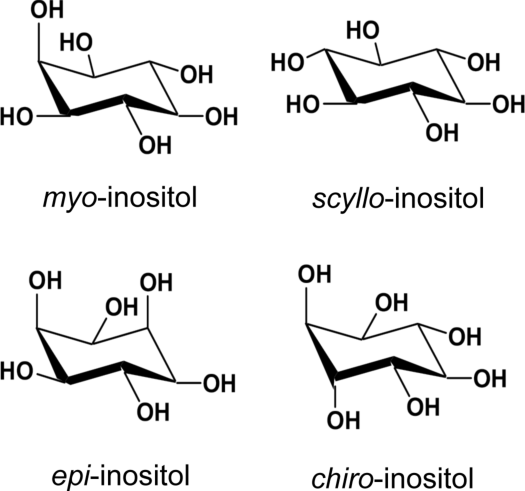
\includegraphics[width=235px]{figures/results1/GA4_paper_figures_submitted-1}
  \caption[Inositol stereoisomers most commonly found in nature.]
   {Stick figures of the stereoisomers were drawn using the ChemDraw software.}
   \label{fig:figure1}
\end{figure}

In vitro, inositol stereoisomers stabilize nonfibrillar β-structure and prevent the formation of amyloid fibrils in a stereochemistry-dependent manner: scyllo-, epi- and myo-inositol inhibit \abeta\ fibril formation, but not chiro-inositol.\cite{McLaurin:2000p64,McLaurin:1998p176,Nitz:2008p13,Sun:2008p12,Townsend:2006p44} Moreover, scyllo-inositol was also demonstrated to be the most effective stereosiomer in preventing and reversing AD-like symptoms in transgenic mice while reducing their brain plaque load.\cite{McLaurin:2006p29} Despite this progress, the molecular basis of amyloid inhibition by inositol is not understood. In vitro studies suggest that inositol stereoisomers affects aggregation through direct interaction with \abeta\ peptides.\cite{McLaurin:1998p176,McLaurin:2000p64,Nitz:2008p13,Sun:2008p12} However, it is not known whether inositol acts on monomeric peptides, non-fibrillar oligomers, or fibrillar aggregates.

Some small molecule inhibitors, including the osmolytes glycerol and trimethylamine N-oxide (TMAO), are known to interfere with in vitro aggregation of amyloidogenic peptides with different sequences,\cite{Scaramozzino:2006p69,Yang:1999p77,McLaurin:2000p76,Ehrnhoefer:2008p8,Dasilva:2010p25,Bieschke:2010p32} suggesting that generic interactions common to all amyloid-forming peptides and proteins may play a role in the inhibition of amyloid formation. Indeed, small organic osmolytes are hypothesized to modulate protein folding equilibria by interacting with the peptidic backbone, the chemical group common to all polypeptides.\cite{Street:2006p21,Hu:2010p46,Auton:2008p28} Accordingly, the role of backbone solvation in the modulation of protein folding\cite{Rose:2006p35,Auton:2008p28} and aggregation equilibria has recently been highlighted.\cite{Rauscher:2006p43} Furthermore, several studies have suggested that N-methylation of the backbone of amyloidogenic peptides can abolish the formation of amyloid fibrils by preventing intermolecular backbone hydrogen bonding.\cite{Takeda:2010p52,Soto:2007p171}

Experimental efforts to characterize the molecular interactions of small molecules with amyloid oligomers and fibrils are often impeded due to the non-crystalline, transient, and disordered nature of the aggregates involved. By contrast, molecular simulations are well-suited for studies of proteins involving disorder.\cite{Rauscher:2010p88} Although several molecular dynamics (MD) simulation studies have begun to examine the effect of small molecules on aggregation and fibril formation,\cite{Takeda:2010p34,Raman:2009p47,Lemkul:2010p23,Liu:2009p18} the role of backbone binding has not been considered systematically.

In this article, we present an MD simulation study of the interaction of inositol with simple model peptides to investigate its stereochemistry-dependent effect on amyloidogenic peptide aggregation and morphology. In a systematic approach, we first characterize the binding equilibria of myo-, epi-, scyllo- and chiro-inositol with alanine dipeptide, a model of the peptidic backbone. Next, to probe the stereochemistry-dependent effect of inositol binding on amyloid aggregation, we study the interaction of scyllo- and chiro-inositol, respectively active and inactive stereoisomers in \abeta\ amyloid inhibition, succcessively with monomer, disordered, and fibrillar aggregates of $(Gly-Ala)_4$ or \gafour. \gafour\ is one of the simplest and shortest amyloidogenic peptides that is known to adopt an extended \bsheet\ structure both synthetically,\cite{Rathore:2001p37} as a metallocopolymer,\cite{Vandermeulen:2006p15} and in nature, in crystalline domains of spider silks.\cite{Kenney:2002p45,Fossey:1991fk} The repetitiveness and simplicity of the peptide sequence allow us to achieve statistically-significant estimates of the binding equilibrium from conventional sampling methods while focusing on the effect of backbone interactions in polypeptide self-aggregation. 

\section{Methods}

\subsection{Simulation Parameters and Protocol}

	Alanine dipeptide (ADP) was methylated at both the N- and C-terminii. The \gafour\ peptide was acetylated and amidated at the N- and C-termini, respectively. The peptides were built using PyMol\cite{Anonymous:2012p58} and modelled using the OPLS-AA/L force field\cite{Jorgensen:1996p19}. The extended OPLS-AA force field for carbohydrates\cite{Damm:1997p36} was used to model inositol stereoisomers and the TIP3P water model\cite{Jorgensen:1983p40} was used to represent the solvent. Versions 3.3.1 and 3.3.3 of the GROMACS software package\cite{VanDerSpoel:2005p56} were used to perform unrestrained all-atom MD simulations with the leap frog algorithm using an integration timestep of 2 femtoseconds. Unless otherwise noted, the following parameters were used for all simulations in this study. Electrostatic interactions were calculated using Particle Mesh Ewald (PME) summation with a grid size of 0.15 nm and a real-space cutoff of 1.45 nm.\cite{Essmann:1995p51} The Lennard-Jones potential was computed up to 1.3 nm and was switched to zero at 1.4 nm using the GROMACS switch function. The temperature and pressure were controlled at 300 K and at 1 atm using the Berendsen thermostat and pressure coupling scheme, respectively.\cite{Berendsen:1984p26} Covalent bonds involving hydrogens were constrained using the SHAKE algorithm.\cite{Ryckaert:1977p30} All resultant simulation systems were first subjected to energy minimization and equilibration with isotropic pressure coupling. Replicas of every system were generated with different random seeds for the choice of initial velocities. A trajectory frame was written to disk every picosecond and all frames were used in the final data analysis. Additional details of simulation setup and total sampling time for all systems performed in this study are listed in Table~\ref{tab:simulations}.
	
	% TODO Change the first column to be left-justified and resized ... HOW?
  \begin{table}\footnotesize
    \begin{center}
    \vspace{10pt}
    \label{tab:simulations}
      \begin{tabular}{| p{2.5cm} | *{7}{p{1.25cm}|}}
        \hline
        System & $N_{peptides}$ & $N_{inositol}$ & $c_{peptide}$ (mM) & $c_{Inositol}$ (mM) & $N_{replicas}$ & Time per replica ($\mu$s) & Total time ($\mu$s) \\
        \hline
        \hline
        alanine dipeptide & 1 & 0 & 61.5 & 0 & 5 & 0.1 & 0.5\\
        with myo-,epi-,chiro- or scyllo-inositol & 1 & 4 & 61.5 & 246 & 5 & 0.1 & 0.5 \\
        \hline
        (GA)4 monomer & 1 & 0 & 61.5 & 0 & 1117 & 0.005 & 5.585 \\
        with chiro- or scyllo-inositol & 1 & 2 & 61.5 & 123 & 1117 & 0.005 & 5.585 \\
        \hline
        (GA)4 disordered aggregate (preformed) & 4 & 0 & 246 & 0 & 5 & 0.1 & 0.5 \\
        with chiro- or scyllo-inositol & 4 & 2 & 246 & 123 & 5 & 0.08 & 0.4 \\
        \hline
        (GA)4 disordered aggregate (dispersed) & 4 & 0 & 246 & 0 & 5 & 0.1 & 0.5 \\
        with scyllo- & 4 & 2 & 246 & 123 & 4 & 0.08 & 0.32 \\
        with chiro- & 4 & 2 & 246 & 123 & 3 & 0.08 & 0.24 \\
        \hline
        (GA)4 fibrillar aggregate & 16 & 0 & 437 & 0 & 3 & 0.1 & 0.3 \\
        with chiro- or scyllo-inositol & 16 & 4 & 437 & 109 & 3 & 0.1 & 0.3 \\
        \hline
      \end{tabular}
      \caption{Summary of simulation systems.}
    \end{center}
  \end{table}

Five initial starting conformations of ADP were obtained by taking a frame every 20 ns from a 100-ns-long simulation of ADP in water. Sets of five independent simulations were carried out successively in the presence of myo-, epi-, chiro- and scyllo-inositol. The initial conformations of monomeric \gafour\ were taken from an ensemble of monomeric structures generated in water at 296 K by simulated tempering distributed replica sampling (STDR) from a previous study.\cite{Nikolic:2011p57} STDR is a generalized-ensemble simulation method developed in our laboratory, which allows each replica in the simulation to undergo a random walk in temperature to enhance conformational sampling.\cite{Rodinger:2006p78} The STDR algorithm and implementation are described elsewhere.\cite{Rauscher:2009p41} A representative set of 1117 structures were chosen from the STDR ensemble at 296 K such that the end-to-end distance probability distribution of this selected subset is similar to the distribution of the entire STDR ensemble of structures (about 12,000 structures in total). These conformations were then used as starting points for simulations at T = 300 K in the presence of two molecules of either scyllo- or chiro-inositol. A total of 5 µs of simulation time was generated for the monomeric systems with either scyllo- or chiro-inositol (Table~\ref{tab:simulations}). The initial peptide conformations of disordered oligomeric systems were either dispersed monomers drawn from the STDR ensemble at 296K or a preformed \bsheet\ oligomer of \gafour\ composed of four peptides.
	The \gafour\ peptide in the extended conformation was constructed using PyMol and was used to create the fibril-like \bsheet\ model. An eight-stranded antiparallel \bsheet\ was constructed by first creating an antiparallel dimer of \gafour. The principal axis of the dimer was then aligned with the x-dimension of the box and translated along the y-axis to form a single 8-stranded \bsheet. Two of these 8-stranded sheets were stacked in parallel in a ``face-to-back" manner (with all Ala methyl groups facing up in the z direction) and placed in the simulation box such that the first strand at the edge of the \bsheets was hydrogen-bonded in-register to the nearest periodic image of the eighth strand. The fibril-like systems were first subjected to energy minimization and a 500 ps equilibration stage. Production simulations were performed in the NVT ensemble with final box dimensions of 4 nm x 3.8 nm x 4 nm. Three independent simulations of the \gafour\ fibril-like systems were performed for 100 ns each, successively in the presence and absence of scyllo- and chiro-inositol (see Table~\ref{tab:simulations}).

\subsection{Analysis Protocol}
	The DSSP geometry criteria\cite{Kabsch:1983p31} were used to determine the presence of a hydrogen bond: (1) the distance between donor (D) and acceptor (A) atoms is less than 0.35 nm; (2) the distance between the hydrogen and A is less than 0.25 nm; and (3) the angle formed by D-H-A is greater than 120°. Nonpolar contacts between inositol and peptide were defined by a separation between the center of mass of inositol and the Cβ atom of alanine less than 0.45 nm. The same cut-off was used to compute protein-protein nonpolar contacts between C$\beta$ atoms.
	All of the dissociation constants for inositol were calculated based on the presence of intermolecular contacts as defined above. Then, assuming that the binding equilibrium of inositol is
	
	% Equations used in the KLVFFAE paper                                                                                                                  
  \begin{equation}
    \left[ Protein\cdot Inositol \right] 
    \rightleftharpoons 
    \left[ Protein \right]+\left[ Inositol \right]
  \end{equation}
  
the dissociation constant is the equilibrium constant of this reaction and is given by 

 \begin{equation}
   K_{d} = f_{ub}\frac{\left[ Protein \right]\left[ Inositol \right]}{\left[Protein \cdot Inositol\right]},
 \end{equation}
 
where fub is the fraction of unbound over bound peptide states.
	 The DSSP algorithm was used for the analysis of secondary structure of the disordered oligomer with N- and C-termini of the peptides excluded. The end-to-end distance for a \gafour\ peptide was calculated as the distance between Cα atoms of the N and C-terminus of the peptide. The spatial probability density of inositol is the average spatial occupancy of the atoms of inositol and was computed using the VolMap tool from the Visual Molecular Dynamics (VMD) software package. %XXX {humphrey, 1996 #143} 
The planar angle between inositol and the fibrillar model of \gafour\ was computed using the g\_sgangle program from GROMACS analysis tools. All planar angles were corrected to a value between 0$\degree$ and 90$\degree$, using the rule $\alpha = f(\theta) = 180 - \theta$, if $\theta$ > 90$\degree$, otherwise, $f(\theta) = \theta$. The probability distribution of the planar angles, P(α), was determined for inositol molecules with atoms within 0.25 nm of the fibril. Average nonpolar and hydrogen bonding contacts in disordered aggregates were computed using the last 70 ns of each trajectory. Error bars were determined by computing the standard deviation of the averages obtained from trajectories of independent replicas. Block averaging was used whenever a single trajectory was available.

\section{Results}

Inositol was found to bind weakly and reversibly to all the peptidic systems considered in our simulations, allowing us to characterize binding equilibria from unbiased sampling.

% This is a table with footnotes and with the footnote rule removed
% It uses the minipage and I had to tweak the width of the page so that center can 
% properly align the table in the middle of the page.
\begin{table}\footnotesize
  \vspace{10pt}
  \label{tab:binding_constants}
  \begin{minipage}{15cm}
    \renewcommand{\thefootnote}{\thempfootnote}
    \renewcommand{\footnoterule}{}
    % \centering
      \begin{center}
    \begin{tabular}{| l | *{5}{ c |}}
       \hline
         System & Scyllo\footnote{Each dissociation constant is in units of mM. The standard error is shown within parentheses.} & Chiro \footnotemark[\value{mpfootnote}] & N$_{groups,ADP}$/N$_{groups}$ & Scyllo \footnote{K$_d$ in units of mM, estimated by scaling the K$_d$ of ADP by the ratio of the number of \\ peptide groups in ADP to the \gafour\ system } & Chiro\footnotemark[\value{mpfootnote}]\\
         \hline
         \hline
         alanine dipeptide & 1100 (100) & 1000 (100) & 1.00 & 1100 & 1000 \\ 
         (GA)4 monomer & 376 (10) & 362 (16) & 0.25 & 275 & 250 \\ 
         (GA)4 preformed & 85 (12) & 89 (8) & 0.06 & 69 & 63 \\ 
         (GA)4 dispersed & 87 (21) & 86 (10) & 0.06 & 69 & 63 \\ 
         (GA)4 fibrillar & 51 (3) & 36 (15) & 0.02 & 17 & 16 \\
         \hline
     \end{tabular}   
  \end{center}
  \end{minipage}
  \centering
  \caption{Summary of equilibrium dissociation constants (K$_d$) for each system in the study.}
  \end{table}


\subsection{Alanine dipeptide}

	Inositol stereoisomers bound weakly and reversibly to alanine dipeptide with a molar Kd. A list of computed dissociation constants for each stereoisomer is shown in Table~\ref{tab:binding_constants}. Because all of the results for myo- (1.0 ± 0.1 M), epi- (1.2 ± 0.2 M), chiro- (1.0 ± 0.1 M) and scyllo-inositol (1.1 ± 0.1 M) were within error bars of one another, in this section we provide detailed descriptions and data only for scyllo-inositol. A single molecule of scyllo-inositol can bind the peptidic backbone in either monodentate or bidentate fashion, as defined by the number of hydrogen bonds between hydroxyl groups of inositol and peptide groups. At a concentration of 250 mM, scyllo-inositol was bound in the monodentate and bidentate modes about 14 ± 1\% and 1.1 ± 0.1\% of the time, respectively. The dominant bidentate binding modes of scyllo-inositol involved hydrogen bonds formed with the peptide main chain either in the mean plane of the inositol ring (Figure~\ref{fig:figure2}, panels I-III) or in a ``face-to-edge" fashion, where the mean plane of the inositol ring is perpendicular to the plane of the peptide groups (Fig. 2A, panel IV).
	
	\begin{figure}[ht]
    \centering
    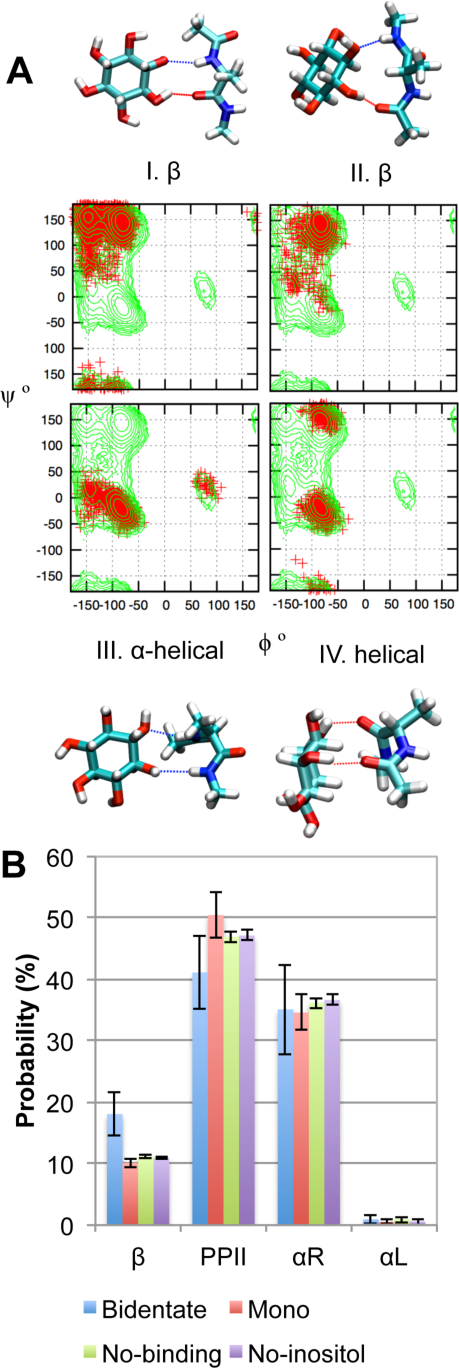
\includegraphics[width=220px]{figures/results1/GA4_paper_figures_submitted-2}
    \caption[Binding of scyllo-inositol to the backbone of alanine dipeptide.]
     {A) Main bidentate binding modes. Ramanchandran maps of the conformations of alanine dipeptide sampled in absence of inositol are shown as contours in green. ($\phi$,$\psi$) of alanine dipeptide conformers bound by inositol are shown on the map as red crosses. $\beta$-conformers (top panels) are bound by inositol through adjacent or non-adjacent (CO,NH) groups; Helical conformers (bottom panels) involve mostly (CO,CO) and (NH,NH) groups. B) Comparisons of the conformational equilibrium of alanine dipeptide for different inositol backbone-bound states.}
     \label{fig:figure2}
  \end{figure}
  
The Ramachandran map of ADP is characterized by four dominant basins representing the α-helical, polyproline II (PPII), and \bsheet\ conformations.\cite{Neale:2008p87} As shown in Fig. 2A, bidentate-bound ADP adopts backbone dihedral angles that fall within the dominant basins on the ramachandran map, demonstrating that scyllo-inositol is able to bind both helical and \bsheet\ conformations. Notably, the conformational equilibrium of ADP is shifted in favor of the β-conformer when scyllo-inositol is bound to the peptide backbone in bidentate fashion (Figure~\ref{fig:figure2_rama} 2B); in contrast, the relative populations of dominant conformers remained unchanged when inositol is unbound or bound in monodentate form. Taken together, our results show that although binding is weak, inositol may influence peptide conformations by binding to the peptidic backbone. In the next sections, we examine the binding of inositol to monomer and aggregates of a simple \bsheet\ forming peptide, \gafour.

\begin{figure}[ht]
  \centering
  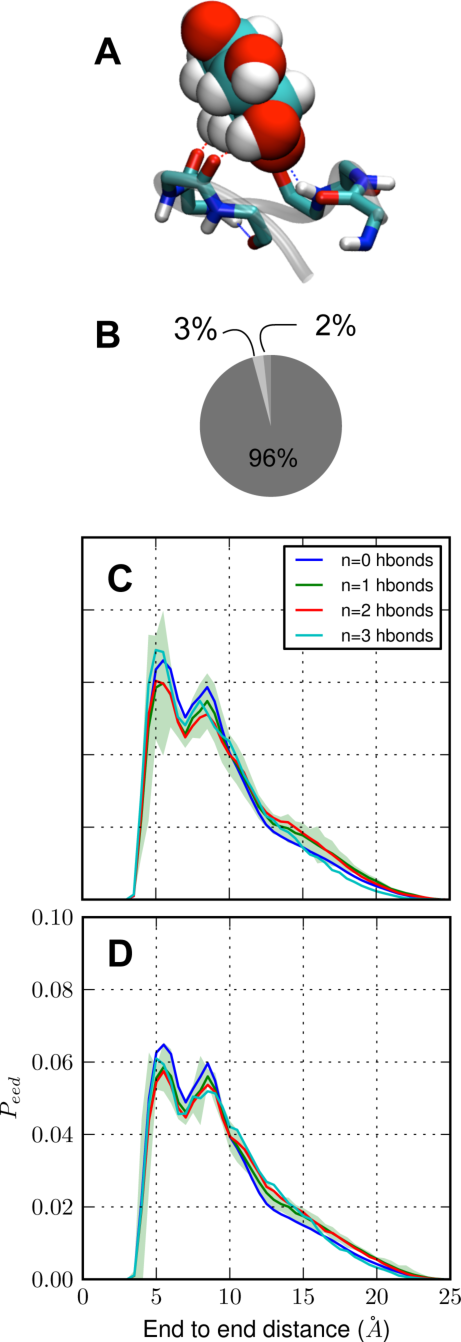
\includegraphics[width=221px]{figures/results1/GA4_paper_figures_submitted-3}
  \caption[Binding of scyllo-inositol to the monomer of (GA)$_4$.]{A) Representative snapshot of scyllo-inositol forming three hydrogen bonds to a monomer of (GA)$_4$. B) Distribution of the fraction of bound scyllo-inositol to polar and nonpolar groups of the monomer. C-D) Conformational equilibrium of (GA)$_4$ as measured by the peptide end-to-end distance distribution. The distributions are all within error bars of each other and are plotted separately by the number of hydrogen bonds for scyllo- in C) and chiro-inositol in D). For clarity, error is only shown for the Peed curve where $n$=1.}
   \label{fig:figure3}
\end{figure}

\subsection{\gafour\ peptide}
In this section, we characterize the binding modes and binding affinity of inositol systematically, first with a peptide monomer, and then with oligomeric and fibrillar aggregates of \gafour. Here we examine only the active and inactive stereoisomers scyllo- and chiro-inositol. A summary of the equilibrium binding constants computed for all \gafour\ systems is shown in Table~\ref{tab:binding_constants}.

\subsubsection{Monomer}

In its monomeric state in solution, \gafour\ is an intrinsically disordered peptide.\cite{Nikolic:2011p57} An example of scyllo-inositol binding to a monomer is shown in Figure~\ref{fig:figure3_mon}A. Similar to ADP, binding is weak: the computed dissociation constants were Kd,chiro ≈ 362 ± 16 mM and Kd,scyllo ≈ 376 ± 10 mM. Most bound states, 95\% for scyllo-inositol and 94.4\% for chiro-inositol, involved hydrogen bonds to the backbone Figure~\ref{fig:figure3_mon}B). At a concentration of 123 mM, inositol molecules formed a single hydrogen bond about 9\% of the time, whereas two or more hydrogen bonds were formed about 4 to 5\% of the time. In contrast, nonpolar contacts are less frequent and, alone, account for only 3\% of bound scyllo- and chiro-inositol (Figure~\ref{fig:figure3_mon}B). In total, the peptide monomer is bound to at least one molecule of inositol approximately 25\% of the time, 23\% of the time with a inositol:peptide stoichiometry of 1:1 and only ~2\% of the time with a 2:1 stoichiometry. Contrary to ADP, the presence of inositol did not have a significant effect on the conformational equilibrium of monomeric \gafour\ (Figure~\ref{fig:figure3_mon}C-D).

\subsubsection{Disordered Oligomer}

\begin{figure}[ht]
  \centering
  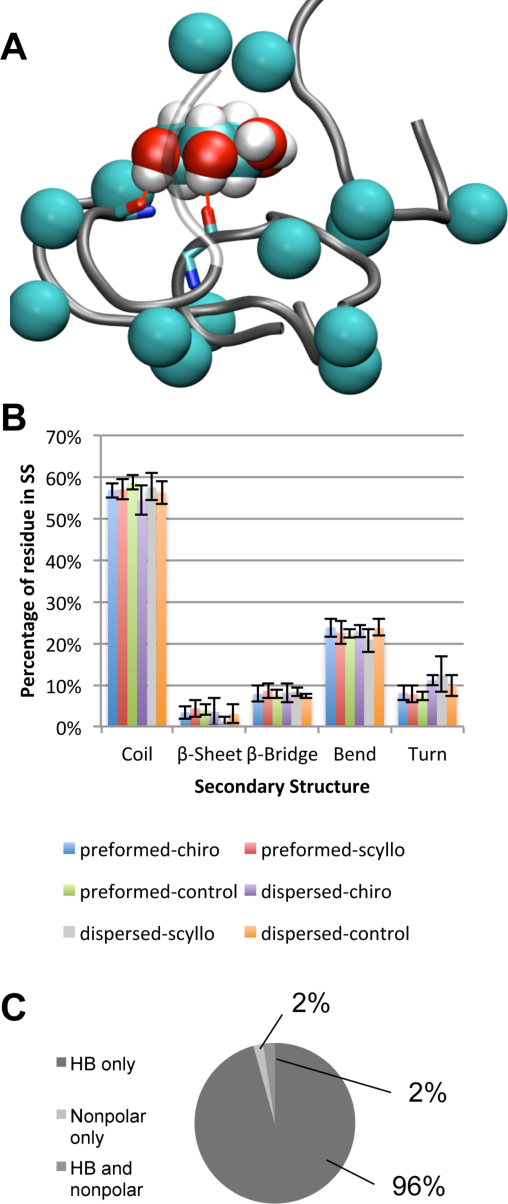
\includegraphics[width=243px]{figures/results1/GA4_paper_figures_submitted-4}
  \caption[Binding of scyllo-inositol to the disordered oligomer of (GA)4.]{A) Snapshot of scyllo-inositol simultaneously hydrogen bonding two peptides in a disordered (GA)4 aggregate. Hydrogen bonds to the backbone are drawn as red lines. B) Distribution of secondary structure content, as classified by the DSSP algorithm, for preformed and dispersed starting states of the oligomer. Hydrogen bonds to the backbone are drawn as red lines. C) Fraction of scyllo-inositol interacting with the disordered oligomer via hydrogen bonds (HBs), nonpolar contacts, or both. The fractions for chiro-inositol are similar (data not shown).}
   \label{fig:figure4}
\end{figure}

	To probe whether inositol affects the structure and aggregation of small oligomers of \gafour\ in solution, we performed sets of simulations involving two distinct starting states of four \gafour\ peptides: (1) initially monodispersed peptides and (2) a preformed \bsheet\ aggregate. In the initially dispersed systems, the peptides rapidly aggregated to form a disordered oligomer (Fig. 4A) in which the majority of the residues (~60\%) retained a coil conformation (Fig. 4B). Similarly, systems initiated with a preformed 4-stranded \bsheet\ also evolved into a disordered oligomer over the course of the simulation. Only about 5\% and 10\% of the residues participated in a \bsheet\ or in a \bbridge, respectively (Fig. 4B).
	
\begin{figure}[ht]
  \centering
  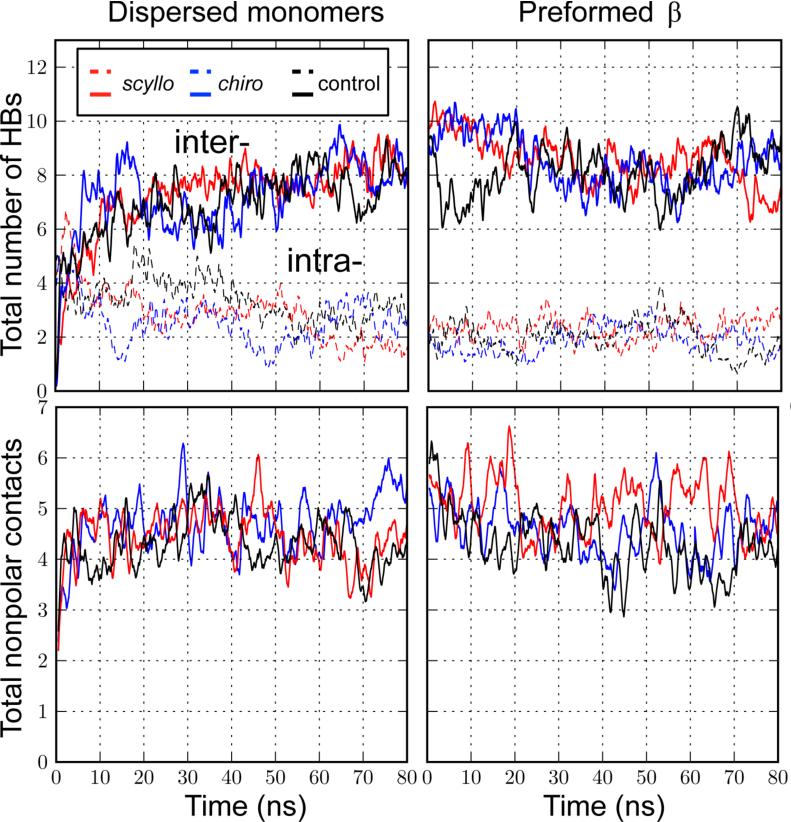
\includegraphics[width=4in]{figures/results1/GA4_paper_figures_submitted-5}
  \caption[Time evolution of peptide-peptide nonpolar and hydrogen bonding contacts in disordered aggregates in presence and absence of inositol (control).]{Each curve is smoothed using a running average over a window with a length of 500 ps. Results for the dispersed monomer aggregates are shown on the left and the preformed β-sheet aggregates on the right. Top: the total number of inter- and intra-molecular hydrogen bonding contacts; Bottom: Number of intermolecular nonpolar contacts.}
   \label{fig:figure5}
\end{figure}
  
Despite different initial conditions and independently of the presence of inositol, all aggregates evolved to a similar morphology. The total number of peptide-peptide nonpolar and polar contacts formed within the oligomer converged to similar values for both the dispersed and preformed oligomers and did not change with time (Figure~\ref{fig:figure5}). As shown in Fig. 5 (top panels), the average total number of intermolecular hydrogen bonds (~8 ± 1) was consistently \bbridge higher than the number of intramolecular hydrogen bonds (~2.1 ± 0.3). On average, about 4.3 ± 0.4 nonpolar contacts were formed upon aggregation in the absence of inositol compared to 4.4 ± 0.5 contacts for scyllo-, and 5.0 ± 0.4 for chiro-inositol (data not shown for the preformed oligomer). When taken together, the above results show that the presence of scyllo- and chiro-inositol neither prevented aggregation nor disrupted the preformed oligomer.
	 Dissociation constants of about 80 mM to aggregates of type 1 and 2 were obtained for both scyllo- and chiro-inositol. The Kd calculated for each aggregate type is shown in Table~\ref{tab:binding_constants}. In the presence of multiple aggregated chains, a single molecule of inositol was found to cross-link multiple peptides by simultaneously hydrogen bonding to their backbones (Fig. 4A). Similar to monomers, at a concentration of 123 mM, chiro- and scyllo-inositol were bound predominantly to the backbone: ~96\% of bound scyllo-inositols formed only hydrogen bonding contacts (~94\% for chiro-inositol), whereas 2\% (3\% for chiro-inositol) were involved in nonpolar contacts only (Figure~\ref{fig:figure4}C).

\subsubsection{Fibril-like oligomer} % (fold)

\begin{figure}[ht]
  \centering
  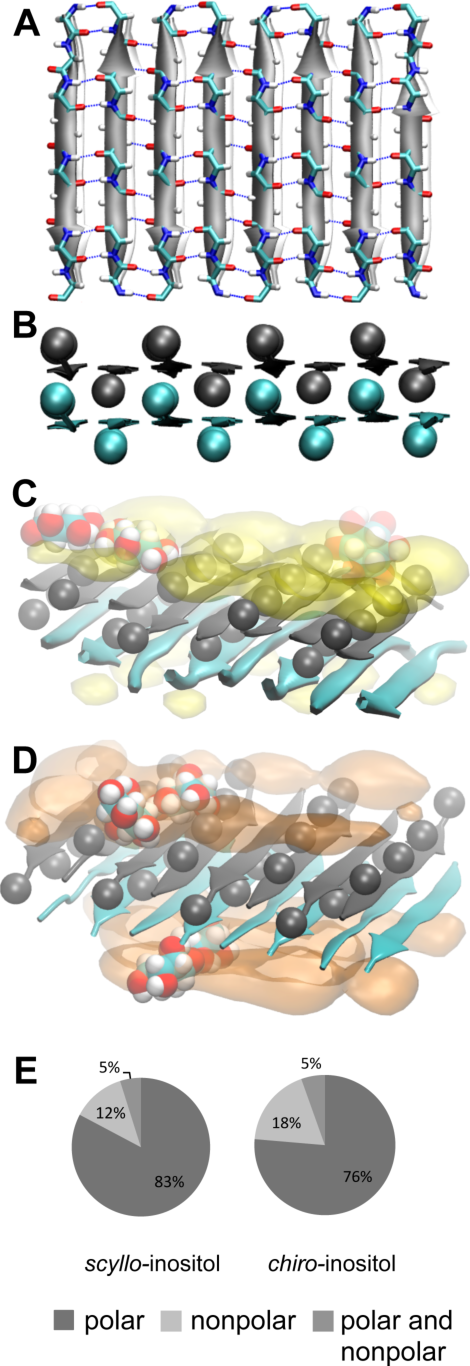
\includegraphics[width=4in]{figures/results1/GA4_paper_figures_submitted-6}
  \caption[Binding of scyllo- and chiro-inositol to the fibrillar aggregate of \gafour.]{Binding of scyllo- and chiro-inositol to the fibrillar aggregate of \gafour. Different views of the initial starting structure of the fibril-like model. Top and bottom sheets are colored in grey and in cyan, respectively. A top down view is depicted in A) showing the backside of the top \gafour\ sheet. A side view of the protofibril is shown in B). The spatial probability density of bound scyllo-inositol (yellow) C) and chiro-inositol (orange) D) are shown overlapping with the fibril. The density is shown at an occupancy isosurface value of 3\% for both stereoisomers. E) is the percentage of bound scyllo- and chiro-inositol to polar and nonpolar groups on the \bsheet.}
   \label{fig:figure6}
\end{figure}

In order to probe the binding modes of inositol with a fibril-like aggregate of \gafour, we constructed an ‘infinite \bsheet’, where the β-strands at the edge of an octameric \bsheet\ are hydrogen-bonded to each other’s nearest periodic image. A single unit of this periodic model consisted of a stack of two antiparallel and in-register \bsheets, with eight strands per sheet (Figs. 6A,B). Although some of the hydrogen bonds defining the \bsheet\ structure occasionally broke, in the absence of inositol the protofibril remained approximately planar and aggregated as an infinite fibril throughout the simulation.
	The spatial distribution of bound inositol molecules shows that both chiro- and scyllo-inositol bind at the surface of the fibril (Fig. 6C, D). Chiro- and scyllo-inositol bound fibrillar aggregates of \gafour\ with a Kd of 36 ± 15 mM and 51 ± 3 mM, respectively. The apparent increase in affinity compared to amorphous aggregates can be attributed to the following reasons. First, the fibrillar aggregate presents a much larger effective surface area than both the monomer and the disordered oligomer (Figs. 6C, D). Moreover, a larger fraction of the alanine side chains are completely solvent-exposed in the fibril-like aggregate, increasing the fraction of bound conformations involving only nonpolar contacts by nearly an order of magnitude, from 2\% in the disordered oligomer to 12\% for scyllo- and 18\% for chiro-inositol in the fibrillar aggregate in the presence of 109 mM of inositol (Figs. 3B and 6E). Accordingly, a higher fraction of scyllo-inositol, 83 ± 1\%, versus 77 ± 1\% for chiro-inositol, was found to form hydrogen bonds, where the 6\% drop in the hydrogen-bonded-only population of chiro-inositol was compensated by a commensurate increase in the nonpolar-bound-only population of chiro-inositol (Fig. 6E).

\begin{figure}[ht]
  \centering
  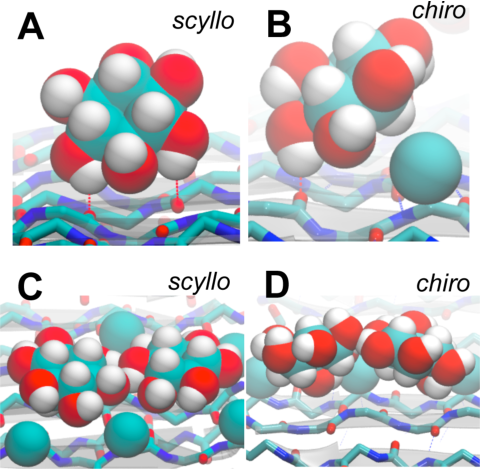
\includegraphics[width=4in]{figures/results1/GA4_paper_figures_submitted-7}
  \caption[Binding of scyllo- and chiro-inositol to the fibrillar aggregate of \gafour.]{Example snapshots of scyllo- and chiro-inositol binding to the fibril of \gafour. Red and blue dashed lines denote hydrogen bonds. A-B) Example binding modes of scyllo- and chiro-inositol binding at an angle to the surface. C-D) Example binding modes of scyllo- and chiro-inositol binding face down on the sheet. }
   \label{fig:figure7}
\end{figure}

\begin{figure}[ht]
  \centering
  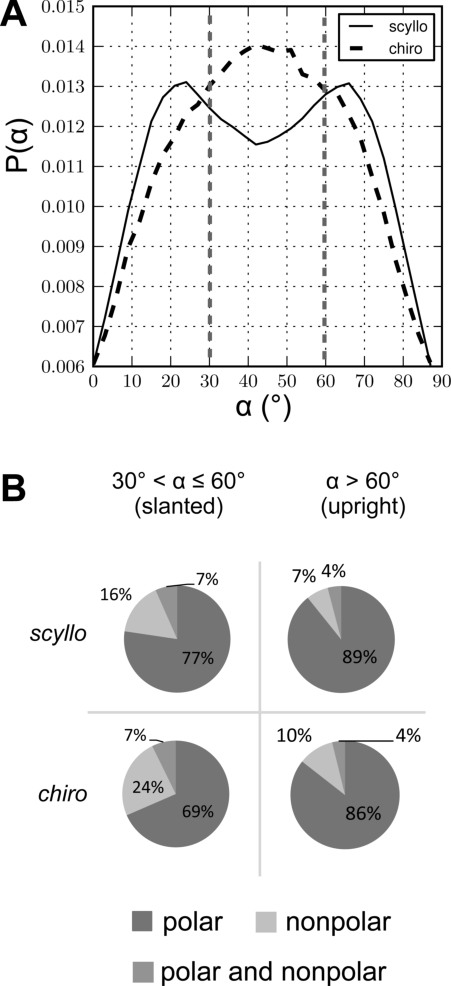
\includegraphics[width=4in]{figures/results1/GA4_paper_figures_submitted-8}
  \caption[Binding mode and orientation of scyllo- and chiro-inositol to the fibril of \gafour.]{Binding mode and orientation of scyllo- and chiro-inositol to the fibril of (GA)4. The distribution of inositol to sheet planar angles is depicted in A). B) Inositol binding to nonpolar and polar groups as classified by α, the angle at which inositol molecules bind at the surface of the fibrillar (GA)4 (see Methods).}
   \label{fig:figure8}
\end{figure}

Thus, although chiro- and scyllo-inositol have similar binding constants, they have different binding modes to fibrillar aggregates, a feature not previously observed for the monomer and the disordered oligomer of \gafour. Both scyllo- and chiro-inositol form nonpolar contacts and backbone hydrogen bonds in poses where the mean plane of the inositol ring lies parallel, at an angle, or perpendicular to the plane of the fibril (Fig. 7). Furthermore, two or more molecules of inositol may cluster together and bind at the surface of the sheet (Figs. 7C,D). However, as shown in Fig. 8A, scyllo-inositol adopts specific binding orientations whereas chiro-inositol does not: scyllo- preferentially binds in either nearly flat (α = 20°) or upright (α = 65°) to the sheet, whereas chiro-inositol does not have such a bimodal preference and binds the fibril at an average angle of α = 45°. This stereochemistry-modulated difference in binding specificity explains the somewhat higher fraction of nonpolar binding by chiro-inositol (Fig. 6E): chiro- is more likely than scyllo-inositol to bind at angles of 30° < α ≤ 60° (Fig. 8A), where 24\% of bound chiro- (versus 16\% for scyllo-inositol) is bound by nonpolar contacts only (Fig. 8B). For α ≤ 30°, the distributions of scyllo- and chiro-inositol bound to polar and nonpolar groups are similar (data not shown). Moreover, because chiro-inositol has a partially-nonpolar edge whereas scyllo-inositol does not, binding in the upright position also involves more nonpolar interactions for chiro- than for scyllo-inositol (Fig. 8B). Finally, although inositol was observed to bind at the surface, binding did not change the morphology of the fibrillar aggregate.


\section{Discussion}
In the above analysis, we have systematically characterized the association of stereoisomers scyllo-, epi-, myo- and chiro-inositol with alanine dipeptide, a simple model of the peptidic backbone. Furthermore, we examined the binding of scyllo- and chiro-inositol to various aggregated states of \gafour\ to probe the role of backbone binding in amyloid inhibition. Our results show that inositol exhibits weak binding with dissociation constants in the range of 0.04 M to 1 M to the different peptides and aggregation states considered.

Furthermore, the Kd of inositol increases linearly with the number of peptide groups in the system (Table~\ref{tab:binding_constants}), indicating that inositol does not bind cooperatively to the monomer and aggregate states of \gafour\ considered. As expected, inositol binds most weakly to alanine dipeptide, with a value about 4 times smaller than the Kd of urea to N-acetyl alanine reported recently in the literature (0.3 M for urea\cite{Lee:2010p59} vs 1.1 M for scyllo-inositol). Taken together, our results indicate that the activity of inositol stereoisomers is similar to that of osmolytes, which typically have binding constants in the millimolar to molar range.\cite{Rosgen:2007p90,Street:2006p21}

Moreover, our results are consistent with the hypothesis that osmolytes influence protein and peptide folding and stability through direct binding rather than by modifying solvent properties.\cite{Canchi:2011p53,Lee:2010p59,Street:2006p21} The spacing of consecutive OH groups of inositol is well-suited to bidentate interactions with adjacent groups of the polypeptide backbone (Fig. 2A). Our findings shown in Fig. 2A are consistent with similar binding modes observed in a recent ab initio simulation and IR spectroscopic study of the binding of glucose epimers to the phenylalanine dipeptide backbone.\cite{Cocinero:2011p54} Furthermore, inositol stereoisomers displace the backbone conformation of alanine dipeptide towards extended β-strand conformations (Fig. 2B). However, neither scyllo- nor chiro-inositol had a significant effect on the conformational equilibrium of the \gafour\ monomer. Taken together, these results indicate that inositol may not act as a drug by directly influencing monomer conformations. However, our results do not preclude the possibility that inositol may block fibril elongation by preferentially binding to monomers that are constrained to extended conformations, such as those at exposed edges of \bsheets.

Independently of the presence of inositol, both the preformed \bsheet\ oligomer and the monodisperse solution of \gafour\ evolved into a similar morphology (Figs. 4B and 5) with only a small amount of β-structure (Fig 4B), indicating that small aggregates of \gafour\ are likely to be disordered. Unlike the hydrophobic core of the \abeta\ peptide, \gafour\ is a shorter and more polar peptide that is capable of forming more hydrogen bonds than nonpolar contacts. Our results show that peptide-peptide hydrogen bonding play an important role in the aggregation of \gafour\ peptides in solution (Fig. 5). Because neither stereoisomer disrupted the aggregates of \gafour, our results indicate that inositol is unlikely to inhibit fibril formation by breaking up preformed aggregates. Therefore, we conclude that inositol is unlikely to inhibit fibril formation by binding monomers and small disordered oligomers since binding appears to be weak, non-cooperative, and stereochemistry-independent.

By contrast, although the dissociation constants were similar for both scyllo- and chiro-inositol, binding specificity and binding modes involving nonpolar groups of the fibrillar aggregate of \gafour\ were modulated by the stereochemistry of inositol. A significantly higher fraction of chiro-inositol than scyllo-inositol was bound to nonpolar groups of the fibrillar aggregate (Fig. 6E). Moreover, scyllo-inositol exhibited a bimodal distribution of binding orientations, with a significant preference for orientations in which the ring of inositol is either parallel or perpendicular to the mean surface of the \bsheet\ over chiro-inositol (Fig. 7). As a direct consequence of the presence of axial hydroxyl groups, chiro-inositol is more likely to bind at angles that promote contact with nonpolar groups at the surface of the fibrillar aggregate, whereas the more specific binding modes of scyllo-inositol favors backbone binding. Since this is the only stereochemistry-dependent result of our study, we speculate that scyllo-inositol acts on ordered \bsheet\ aggregates (as opposed to disordered oligomers or monomers). Moreover, these findings suggest a possible mechanism of action whereby a significant binding affinity to specific side chains on the surface of fibrillar aggregates could lead to the inhibition of \bsheet\ stacking (and therefore, amyloid fibril growth or maturation) by scyllo-inositol. Similarly, different binding modes observed in MD simulations of \abeta42 fibrils have been proposed to explain differences in binding affinities between Thioflavin T, a well-known amyloid-binding dye, and its chemical analogs.\cite{Mathis:2003p55,Wu:2011p24}

A factor that we have not considered in this study is the influence of inositol:peptide molar ratio on binding and inhibition. In vitro, the inhibition activity of scyllo-inositol was observed at an inositol:peptide ratio of 25:1, where inositol stereoisomers were present in excess of \abeta\ at concentrations of 0.25 mM to 5 mM.\cite{McLaurin:2000p64} Although our simulations had effective concentration of inositol an order of magnitude higher than in these experiments, it is possible that we have precluded cooperative inositol binding modes by limiting the number of inositol molecules present in the small simulation cell. Furthermore, Kd values obtained from our simulations of \gafour\ were approximately two orders of magnitude higher than measured for \abeta. Based on our results, the predicted Kd of (GA)21, a Gly-Ala repeat peptide similar in length to \abeta, would be 1200 mM/21 = 57 mM, which is still an order of magnitude greater than in vitro inhibitory concentrations. This indicates that scyllo-inositol is unlikely to inhibit \bsheet\ formation by \gafour\ peptides, and more importantly, that backbone binding by small molecules may not be sufficient for inhibition of amyloid formation. In future studies, elucidating the relationship of binding cooperativity and amyloid inhibition by approaching experimental drug:protein molar ratios, as well as elucidating the sequence specificity of inositol binding to amyloid fibrils, will provide further insight that may be used in the rational drug design of improved inhibitors.

\section{Conclusions}
We have performed systematic simulations of simple amyloidogenic peptide models with both active and inactive stereoisomers of inositol to examine the molecular basis of amyloid inhibition. Our results indicate that although peptide backbone dominates the interaction with inositol, the binding affinity is low and remains in the millimolar range. Moreover, this property is independent of stereochemistry and does not appear to be sufficient to impede peptide dimerization through intermolecular backbone hydrogen bonding. Taken together, our results suggest that amyloid inhibition by inositol cannot be accounted for by generic binding to the peptidic backbone alone and is likely to involve sequence-specific interactions with amino-acid side chains as well as binding to specific aggregate morphologies. Accordingly, although the formation of intermolecular hydrogen bonds is the predominant interaction in protein aggregates composed of \gafour, amyloidogenic peptides involved in amyloid diseases are often more hydrophobic and in general, self-aggregation is driven largely by the hydrophobic effect.\cite{Chiti:2006p20} In forthcoming studies, we will examine the role of sequence-specific interactions between inositol and aggregates of pathogenic peptides.

\section{Acknowledgements}
This work was made possible by the Centre for Computational Biology at the Hospital for Sick Children, the facilities of the Shared Hierarachical Academic Research Computing Network(SHARCNET, www.sharcnet.ca), the GPC supercomputer at the SciNet HPC Consortium and Compute/Calcul Canada. This work was supported in parts by a fellowship from the Heart and Stroke Foundation of Ontario, a Canada Graduate Scholarship from the National Science and Engineering Research Council, the Research Training Center at the Hospital for Sick Children, and the Canadian Institutes of Health Research (Grant No. MOP84496). R.P. is a CRCP chairholder.

\addcontentsline{toc}{section}{Bibliography}
\bibliographystyle{plain}
\bibliography{/Users/grace/github/thesis/document/results1/results1}


% % KLVFFAE
% \chapter[Molecular Mechanism of Amyloid Inhibition by Inositol]
{Binding Mechanism of Inositol Stereoisomers to Monomers and Aggregates of A$\beta$(16-22)}

The contents of this section were adapted from an article published in the \emph{Journal of Physical Chemistry}.
\\
\\
\emph{Reference}:
Li, G., Rauscher, S., Baud, S., & Pom\`{e}s, R. (2012). Binding of Inositol Stereoisomers To Model Amyloidogenic Peptides. Journal of Physical Chemistry B, 116(3), 1111–1119.
\\
\\
\emph{Contributions}:
Grace Li conducted the research and wrote the section. R\'{e}gis Pom\`{e}s provided editorial input and guidance.

\newpage

\section{Summary}
Alzheimer's disease (AD) is a severe neurodegenerative disease with no cure. A potential therapeutic approach is to prevent or reverse the amyloid formation of A$\beta$42, a key pathological hallmark of AD. We examine the molecular basis for stereochemistry-dependent inhibition of the formation of A$\beta$ fibrils \emph{in vitro} by a polyol,  \emph{scyllo}-inositol. We present molecular dynamics simulations of the monomeric, disordered aggregate, and protofibrillar states of A$\beta$(16-22), an amyloid-forming peptide fragment of full-length A$\beta$, successively with and without \emph{scyllo}-inositol and its inactive stereoisomer \emph{chiro}-inositol. Both stereoisomers bind monomers and disordered aggregates with similar affinities of 10--120 mM, whereas binding to $\beta$-sheet-containing protofibrils yields affinities of 0.2--0.5 mM commensurate with \emph{in vitro} inhibitory concentrations of \emph{scyllo}-inositol. Moreover,  \emph{scyllo}-inositol displays a higher binding specificity for phenylalanine-lined grooves on the protofibril surface, suggesting that  \emph{scyllo}-inositol coats the surface of A$\beta$ protofibrils and disrupts their lateral stacking into amyloid fibrils.\\
% Refine -- is this statement important?  Carbohydrate is coming out of the blue ..
% Also confusing to say that inositol modulates nonpolar interactions with glutamate ...
% Furthermore, inositol adopts carbohydrate-like binding modes, where stereochemistry modulates the nonpolar binding specificity of inositol to glutamate and phenylalanine side chains. 

\section{Introduction}
One in eight people over the age of 65 has Alzheimer's Disease (AD), a progressive neurodegenerative disease that currently has no cure.\cite{Citron:2010p214} The amyloid cascade hypothesis states that the extracellular neuronal deposition of A$\beta$ amyloid plaque plays a central role in the pathogensis of AD.\cite{Solomon:2010p177} A$\beta$ is a peptide proteolytically cleaved from the amyloid precursor protein and is produced as two common alloforms, A$\beta$40 or A$\beta$42, which are 40 and 42 residues in length, respectively. In the diseased state, A$\beta$42 levels are elevated and the peptides deposit as extracellular A$\beta$ plaques.\cite{Haass:2007p226,Westaway:1997p4185}

A$\beta$40 and A$\beta$42 are intrinsically-disordered peptides that self-aggregate \emph{in vitro} to form amyloid fibrils. Amyloid fibrils are protein aggregates with a characteristic cross-$\beta$ structure, which consists of in-register $\beta$-sheets with backbone hydrogen bonds running parallel to the long axis of the fibril.\cite{Petkova:2002p192} Moreover, smaller fragments of the full-length A$\beta$ sequence are also found to form amyloid \emph{in vitro}.\cite{Balbach:2000p49,Sawaya:2007p11} In particular, one of the shortest amyloid-forming peptides structurally characterized using solid-state NMR is KLVFFAE or A$\beta$(16-22).\cite{Balbach:2000p49} The residues LVFFA are believed to form the central hydrophobic core critical for the initiation of aggregation and fibril formation in the full-length A$\beta$ peptide.\cite{Wood:1995p190} Furthermore, single-point mutations in this region greatly affect the aggregation propensity of A$\beta$: familial mutations E22Q, E22K, and E22G, known as ``Dutch'', ``Italian'', and ``Arctic'' mutations, respectively, significantly accelerate fibril formation,\cite{Kim:2008ef} whereas the mutation F19T abolishes the formation of fibrils \emph{in vitro}.\cite{Esler:1996p288}
% check the different mutations, might be missing one

Amyloid fibril formation follows a complex pathway: prior to the appearance of fibrils \emph{in vitro}, amyloidogenic monomers self-aggregate into a variety of pre-fibrillar intermediate morphologies. While the fibril is an important state implicated in AD, recent research has shown that soluble oligomers as small as dimers and tetramers play a role in neurotoxicity.\cite{Bernstein:2009p165} In recent years, drug development and research efforts have been directed toward the development of therapeutic agents to prevent the self-aggregation and amyloid formation of A$\beta$, a promising treatment approach to target the underlying disease.\cite{Masters:2006p183,Citron:2010p214,Dasilva:2010p25} As a result, many different types of \emph{in vitro} amyloid inhibitors have been discovered, including peptides,\cite{EsterasChopo:2008p219,Sciarretta:2006p181,Chalifour:2003p161,Scrocchi:2002p178,Soto:2007dm} immunotherapies,\cite{Janus:2000p198,Solomon:2010p177} polyphenolic molecules,\cite{Masuda:2009p205,Berhanu:2010p230,Ehrnhoefer:2008p8} and other small molecules.\cite{Hawkes:2009p189,Masuda:2009p205,Necula:2007p227,Nitz:2008p13} These approaches have been reviewed in detail elsewhere.\cite{Citron:2010p214,Dasilva:2010p25}

\emph{scyllo}-Inositol is a small-molecule inhibitor of A$\beta$-fibrillation developed for the treatment of AD.\cite{McLaurin:2006p29,McLaurin:2000p64,Fenili:2007p182,Ma:2012jk} Inositol is a class of cyclohexylpolyols, of which eight out of nine stereoisomers are commonly found in nature. \emph{scyllo}-Inositol, with all hydroxyl groups equatorial,  is the only isomer with two planar hydrophobic faces. By contrast, its diastereisomer, \emph{chiro}-inositol, with two adjacent axial hydroxyl groups, has two nonplanar  hydrophobic faces. \emph{myo}-Inositol, the most common inositol stereoisomer, is found at high concentrations ($\sim$5 mM) in the tissues of the human central nervous system (CNS).\cite{Fisher:2002p62} Like \emph{myo}-inositol, \emph{scyllo}-inositol is present in the brain and can be passively and actively transported across the blood-brain barrier.\cite{Fenili:2007p182} Importantly, \emph{scyllo}-inositol was demonstrated to prevent and reverse AD-like symptoms in a transgenic mouse model of AD.\cite{McLaurin:2006p29} Because of the positive CNS bioavailability and favorable \emph{in vivo} toxicity profile of inositol, both of which are rare and essential properties of putative AD drug candidates, inositol-based therapies represent a unique and promising approach for the treatment of AD. Phase II of clinical trials for \emph{scyllo}-inositol (ELN0005) in North America was fast-tracked in 2007 by the United States Food and Drug Administration and was completed in 2011.\cite{Salloway:2011im,Ma:2012jk}

\emph{In vitro}, inositol displays stereochemistry-dependent inhibition of A$\beta$42 fibrils: \emph{myo}-, \emph{epi}- and \emph{scyllo}-inositol were shown to inhibit A$\beta$42 fibrillation at concentrations of 1--5 mM,\cite{McLaurin:2000p64} whereas \emph{chiro}-inositol is inactive below molar concentrations.\cite{Janus:2000p198} Moreover, upon incubation of monomeric A$\beta$42 with \emph{scyllo}-inositol, circular dichroism spectroscopy indicated the formation of $\beta$-sheet structure at an inositol:peptide molar ratio of 25:1.\cite{McLaurin:2000p64} Although inositol stereoisomers have been proposed to inhibit amyloid formation by directly interacting with either monomers or non-fibrillar aggregates to ``cap off'' fibril growth,\cite{Janus:2000p198} the molecular basis of the effect of \emph{scyllo}-inositol and its stereoisomers on A$\beta$ amyloid formation is currently unknown.

Thus far, experimental efforts to characterize the molecular structure of non-fibrillar oligomers have been impeded by their transient and disordered nature. In turn, the lack of information on the molecular structure of amyloid oligomers hampers experimental determination of the modes of action of inositol. Molecular dynamics (MD) simulations, by contrast, are well-suited for studies of disordered proteins and can provide atomic-level insight into the mechanism of peptide self-aggregation.\cite{Nikolic:2011p185,Rauscher:2006p43,Li:2012p853,Rauscher:2010p5682,Sgourakis:2011hy,Wang:2005do,Cino:2011ff}

MD simulations were previously employed to examine the binding mechanism of other small-molecule inhibitors such as polyphenols,\cite{Lemkul:2010p23,Wang:2010p204} non-steroidal anti-inflammatory drugs\cite{Raman:2009p47,Takeda:2010p34}, and the well-known amyloid dye thioflavin T\cite{Wu:2008ds,Wu:2011fd} to monomers and/or fibrillar forms of A$\beta$\cite{Liu:2009p213}. Because of the existence of multiple aggregation states, small-molecule inhibitors may have multiple modes of action and may act by binding either to monomers\cite{Ehrnhoefer:2008fd} or to non-fibrillar or fibrillar oligomers\cite{Buell:2010p9457} in the fibrillation pathway. Furthermore, their inhibitory activity may also be affected both by the concentration of the ligand and by the ligand:peptide molar ratio. For example, it has been suggested that the ability of small molecules (--)-epigallochatechin gallate (EGCG)\cite{Wang:2010p204} and ibuprofen\cite{LeVine:2005cv} to inhibit amyloid fibrillation is modulated by the ligand:peptide molar ratio.  However, thus far, few MD simulation studies have examined the effect of ligand concentration on different relevant aggregation states along the amyloid fibrillation pathway.\cite{Wang:2010p204}

In a previous study,\cite{Li:2012p853} we investigated the stereochemistry-dependent binding of inositol with alanine dipeptide, a model of the peptide backbone, and (GA)$_4$, a simple $\beta$-sheet-forming peptide. Weak binding, with equilibrium constants (0.04--1 M) commensurate with those of osmolytes, was found for inositol with both peptides and all aggregation states considered, indicating that backbone binding alone is likely to be insufficient for amyloid inhibition. However, that study uncovered stereochemistry-dependent binding modes between inositol and nonpolar groups on the surface of (GA)$_4$ fibril-like aggregates, which suggests that both aggregate morphology and sequence-specific interactions could play an important role in A$\beta$-aggregation inhibition by inositol.  

In this paper, we consider the role of sequence-specific interactions of inositol by examining its binding to A$\beta$(16-22), an amyloidogenic peptide that is part of the central hydrophobic core of fibrillar A$\beta$42.  Because the amyloidogenic species with which inositol may interact are not known, we successively examine its binding to three different morphologies: monomer, disordered oligomer, and protofibrillar-like aggregate ($\beta$-oligomer).  Using a systematic comparative approach, MD simulation studies of each of the aforementioned states are successively carried out in the presence and absence of \emph{scyllo}-inositol and its inactive stereoisomer, \emph{chiro}-inositol.  Moreover, we examine the effect of varying inositol:peptide molar ratios on the binding equilibria of inositol to monomers and aggregates of A$\beta$(16-22). From a total of 24.5 $\mu$s of simulation, we compute binding constants ($K_{eq}$) and characterize the binding modes of inositol to the different peptide aggregation states considered. The results of our study have implications for the mechanism of amyloid inhibition by small molecules and for the rational design of more efficacious putative therapeutics for AD and related amyloid disorders.

%\begin{table}\footnotesize\centering
%    \begin{center}
%    \vspace{10pt}
%    \caption{Summary of simulation systems}
%    \label{tbl:simulations}
%      \begin{tabular}{|>{\centering}p{3cm} | >{\centering}*{7}{p{1cm}<{\centering}|}}
%        \hline
%        System & $N_{peptides}$ & $N_{inositol}$ & $c_{peptide}$ (mM) & $c_{Inositol}$ (mM) & molar ratio & $N_{replicas}$ & Total time ($\mu$s) \\
%        \hline
%        \hline
%        monomer (STDR)		 & 1 & 0   & 61.5     &  0      & -       & 33   & 3.56 \\
%        monomer 				 & 1 & 0   & 4.5       &  0      & -       & 1117   & 5.59 \\
%        \hline
%        \multirow{2}{*}{\parbox{2.5cm}{with \emph{chiro}- or \emph{scyllo}-inositol}}  & 1 & 2   & 61.5   & 123   & 2:1    & 1117  & 5.59 \\
%         						 & 1 & 15   & 4.5   & 70     & 15:1  & 1117  & 8.25 \\
%        \hline
%        \hline
%        disordered aggregate 		 & 4 & 0   & 104 & 0     & -       & 8 & 1.44 \\
%        \hline
%        \multirow{2}{*}{\parbox{2.5cm}{with \emph{chiro}- or \emph{scyllo}-inositol}} & 4 & 2   & 104 & 52   & -       & 5 & 1.00 \\
%                        			 	 & 4 & 15 & 18   & 70   & 15:4   & 8 & 1.44\\
%                                			 %& 4 & 45 & 18   & 209 & 45:4 & 5 & 1.00 \\
%        \hline
%        \hline
%       $\beta$-oligomer & 16 & 0 & 148 & 0     & -     & 1   & 0.13 \\
%        \hline
%        \multirow{3}{*}{\parbox{2.5cm}{with \emph{chiro}- or \emph{scyllo}-inositol}} & 16 & 4 & 148 & 37   & 4:16 & 18  & 0.54 \\
%						 & 16 & 64 & 15 & 62   & 64:16 & \hl{6}   & \hl{0.60} \\
%						 & 16 & 64 & 52 & 208 & 64:16 & \hl{6}   & \hl{0.60} \\
%        \hline
%      \end{tabular}
%    \end{center}
%  \end{table}

\section{Materials and Methods}

\subsection{Simulation Parameters and Protocol}

To eliminate terminal charge effects, the A$\beta$(16-22) peptide was acetylated and amidated at the N- and C-termini, respectively. The peptide was represented by the OPLS-AA/L force field.\cite{Jorgensen:1996p19} The extended OPLS-AA force field for carbohydrates\cite{Damm:1997p36} was used to model inositol stereoisomers. The TIP3P water model\cite{Jorgensen:1983p40} was used to represent the solvent. To mimic \emph{in vitro} fibrillation conditions used in the study by Balbach \emph{et al.}\cite{Balbach:2000p49}, no salt was added to the aqueous solution.  All MD simulations were performed in the \emph{NpT} ensemble using the GROMACS simulation package,\cite{Hess:2008p264,VanDerSpoel:2005p56} versions 3.3.x and 4.0.x. Unless otherwise noted, the following parameters were used for all simulations in this study. The leapfrog Verlet integration algorithm was used with an integration time step of 2 fs. Long-range electrostatic interactions were calculated using Particle Mesh Ewald summation with a Fourier grid spacing of 0.15 nm and a real-space cutoff of 1.3 nm.\cite{Darden:1993p266} The short-range nonbonded van der Waals interactions were switched to zero from 1.1 to 1.2 nm. The temperature was controlled at 300 K using the Berendsen barostat.\cite{Berendsen:1984p26} Pressure was controlled by the Berendsen thermostat at 1 atm with a coupling constant of 1.0 ps.\cite{Berendsen:1984p26} The SHAKE algorithm was used to constrain covalent bonds containing hydrogens.\cite{Ryckaert:1977p30} In all simulations, a cubic box was used with periodic boundary conditions. Prior to data collection, 500 steps of energy minimization were first performed using the conjugate-gradient algorithm, followed by equilibration with isotropic pressure coupling. The center of mass (COM) rotation and translation were removed at every step. 

Molecular simulations of monomeric A$\beta$(16-22) in water were performed in the absence of inositol using the simulated tempering distributed replica sampling algorithm (STDR).\cite{Rauscher:2009p166} STDR is a generalized-ensemble simulation method that allows each replica in the simulation to undergo a random walk in temperature to enhance conformational sampling.\cite{Rauscher:2009p166,Rodinger:2006p78} The STDR simulation was performed using 33 replicas undergoing canonical sampling (\emph{NVT} ensemble) at exponentially-spaced temperatures ranging from 280 to 694 K. A total of 108 ns of simulation at each temperature were generated using Langevin dynamics (implemented by the stochastic dynamics integrator in GROMACS 3.3.x), for a total simulation time of 3.564 $\mu$s. 

A set of 1117 structures was drawn randomly from STDR simulations such that the probability distribution of the end-to-end distance of these peptides closely approximated that of the equilibrium ensemble of KLVFFAE at 296 K. These structures were used as starting points for constant-temperature MD simulations (\emph{NpT} ensemble) in the presence of 123 mM inositol at an inositol:peptide molar ratio of 2:1. Short, 5-ns MD simulations were performed for each structure in the presence and absence of inositol at $T=300$ K. In addition, 15 ns of simulation in the presence of \emph{scyllo}- or \emph{chiro}-inositol molecules at inositol:peptide molar ratios of 15:1 were performed using each of 550 structures drawn randomly from the larger set of 1117 structures.

Total sampling times of 1.44 and 1.5 $\mu$s were generated for disordered aggregates and $\beta$-oligomers of A$\beta$(16-22), respectively. Each of the disordered aggregate simulations was initiated from four peptide conformations drawn at random from the pool of structures obtained at $T=296$ K from the STDR simulation of the monomer. Peptides were initially monodisperse and placed approximately equidistant from each other in the simulation box. Successively 2, 15, and 45 molecules of inositol were added at inositol:peptide molar ratios of 1:2, 15:4, and 45:4, respectively.

The A$\beta$(16-22) $\beta$-oligomer consists of two eight-stranded antiparallel $\beta$-sheets stacked in a ``face-to-face'' and antiparallel manner and was constructed based on solid-state NMR evidence\cite{Balbach:2000p49} using a method similar to that described in our previous study.\cite{Li:2012p853} Consistent with the experimental study, the $\beta$-sheets were stacked so that charged side chains, lysine (Lys) and glutamate (Glu), are located on the solvent-exposed faces of the $\beta$-oligomer.

Simulations of the $\beta$-oligomer were performed successively in the presence of  \emph{scyllo}- and  \emph{chiro}-inositol at inositol:peptide molar ratios of 4:16 and 64:16  using six A$\beta$(16-22) $\beta$-oligomer structures each taken from every 10 ns of a 100-ns long trajectory in the absence of inositol. Simulations at the lower molar ratio of 4:16 were performed at a concentration of 37 mM. For the higher molar ratio, two separate sets of simulations were performed, one at an inositol concentration of 62 mM (approximately the concentration of the low-molar-ratio simulations) and the other at 208 mM, corresponding, respectively to 15 and 64 molecules of inositol in the simulation cell (Table~\ref{tbl:simulations}).  A summary of the production runs used for the analysis of all systems investigated in this study is provided in Table~\ref{tbl:simulations}.

\subsection{Analysis Protocol}

The binding reaction of inositol defined by 
\[\left[ Protein\cdot Inositol \right] \rightleftharpoons \left[ Protein \right] +\left[ Inositol \right], \]
has an associated equilibrium constant of 
\[ K_{eq} = \frac{\left[ Protein \right]\left[ Inositol \right]}{\left[Protein \cdot Inositol\right]}.\] 

The equilibrium constant for inositol binding, $K_{eq}$, was calculated based on the presence of intermolecular contacts (either hydrogen bonding or nonpolar) as defined below. The DSSP hydrogen-bonding criteria were used to determine the presence of a hydrogen bond: (1) the distance between donor and acceptor atoms is less than 0.35 nm; (2) the distance between the hydrogen and the acceptor is less than 0.25 nm; and (3) the angle formed by the donor, hydrogen, and acceptor is greater than 120$\degree$.\cite{Kabsch:1983p31} % Nonpolar contacts between inositol and the peptide were defined by the distance between the center of mass of inositol and the carbon atoms of side chains. 

Nonpolar contacts between inositol and peptide were calculated by considering all nonpolar carbon atoms of amino-acid side chains and carbon atoms of inositol within 0.45 nm and were normalized by the number of peptides present in the system. The total number of intermolecular peptide-peptide nonpolar contacts was calculated by considering all side chain carbon atom pairs within 0.45 nm. 

The potential of mean force (PMF) for the binding of  \emph{scyllo}-inositol and  \emph{chiro}-inositol to phenylalanine (Phe) side chains was computed using two reaction coordinates: (1) the distance between the center of mass (COM) of inositol and the COM of the Phe side chain (excluding the C$_{\beta}$ atom), $r$; and (2) the angle between the mean plane of the cyclohexane ring of inositol and that of the benzene ring of Phe, $\theta$. A molecule of \emph{scyllo}-inositol is considered to be stacked to Phe if $\theta$ < 20$\degree$ and $r$ < 0.45 nm. The PMF is given by $\mathit{W(r, \theta)}=-RT\ln\rho\left(r,\theta\right)$, where $R$ is the gas constant, $T$ is the temperature, and $\rho\left(r,\theta\right)$ is the probability distribution of $r$ and $\theta$. All error bars were estimated using block averaging or by computing the standard deviation in the mean of the property of interest over all independent simulations.

Inositol clusters were computed using the g\_clustsize analysis tool from the GROMACS software package using an atomic cutoff of 0.35 nm. The DSSP algorithm was used for the analysis of the secondary structure of the disordered oligomer with the N- and C-termini of the peptides excluded. The distance between the first and last C$_{\alpha}$ atoms of the peptide chain defines the end-to-end distance. The spatial probability density of inositol was computed using the VolMap tool from the Visual Molecular Dynamics (VMD) software package.\cite{Humphrey:1996p850}

\section{Results}

In the sections below, we successively characterize the binding equilibrium of inositol and its effect on the morphology of monomers and of disordered and protofibrillar oligomers of A$\beta$(16-22).

\subsection{Monomer}

We performed simulations of an A$\beta$(16-22) monomer successively in pure water and in the presence of \emph{scyllo}- and \emph{chiro}-inositol at inositol:peptide molar ratios of 2:1 and 15:1.  These molar ratios were chosen such that the corresponding inositol:residue ratios are above (2:1) and below (<1:1) the inositol:residue molar ratio at which inhibition of A$\beta$42 fibrils was observed \emph{in vitro}.\cite{McLaurin:2000p64}

%\begin{figure}
%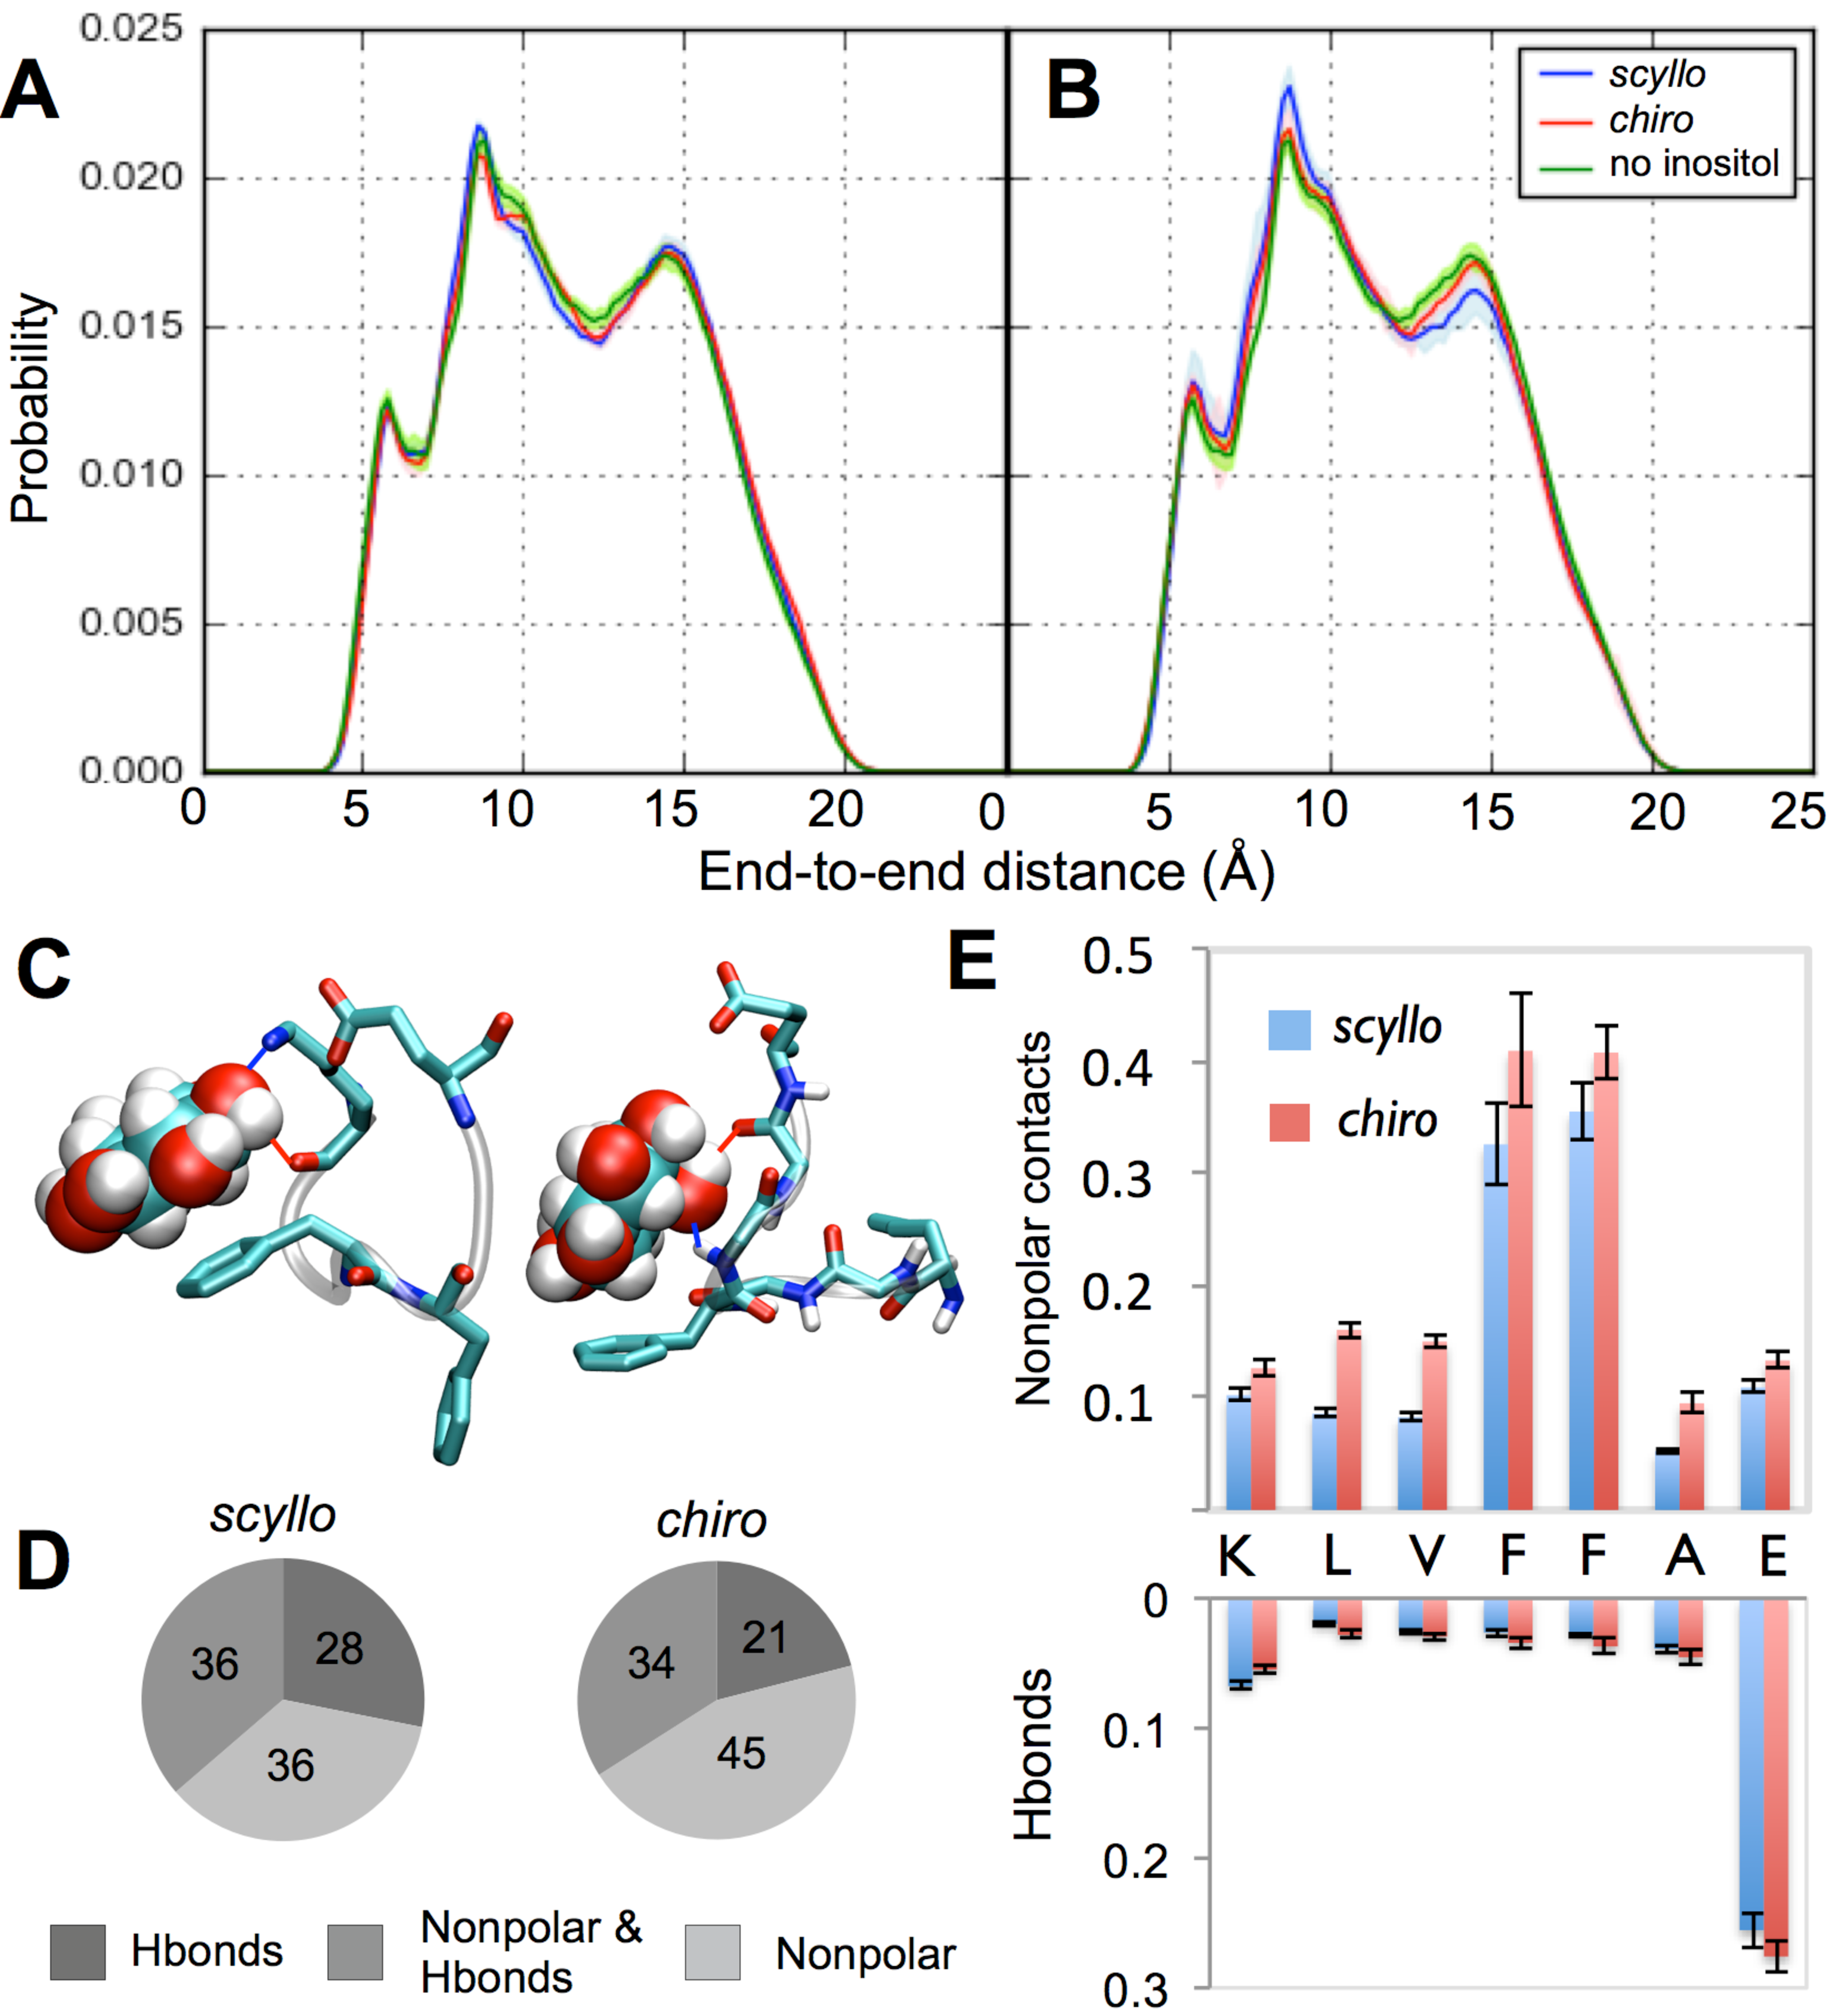
\includegraphics[width=14.6cm]{figures/inos2_figures_monomers_revised.pdf}
%\caption{Binding of inositol to an A$\beta$(16-22) monomer.  End-to-end probability distribution of A$\beta$(16-22) successively in pure water and in presence of \emph{scyllo}- and \emph{chiro}-inositol at inositol:peptide molar ratios of (A) 2:1 and (B) 15:1.  (C) Representative snapshots of the different binding modes of \emph{scyllo}- (left) and \emph{chiro}-inositol (right)  to the peptide monomer. Hydrogen bonds between inositol and backbone NH (blue) and CO (red) groups are shown as solid lines. (D) Percent of bound inositol molecules in contact with nonpolar and polar groups at an inositol:peptide molar ratio of 15:1. (E) Time-averaged number of nonpolar contacts (top), and hydrogen bonds (bottom) made by inositol  (\hl{at a molar ratio of 15:1}) to each residue.}
%\label{fig:monomers}
%\end{figure}

Independent of the presence of inositol, A$\beta$(16-22) is a disordered peptide in solution (Figure~\ref{fig:monomers}A,B) and is able to adopt both collapsed and extended states over the time scales of our simulation. The conformational equilibrium of A$\beta$(16-22), as measured by peptide end-to-end distance distributions, was unaffected by the presence of inositol at both inositol:peptide molar ratios considered (Figure~\ref{fig:monomers}A,B). The three peaks correspond to different intramolecular hydrogen-bonding arrangements (see Figures~\ref{fig:SI-monomersEedByHbonds} and \ref{fig:SI-monomersConformations} in the Supporting Information).\sethlcolor{yellow}

Inositol molecules bound weakly and reversibly to the monomer of A$\beta$(16-22). Representative examples of \emph{scyllo}- and \emph{chiro}-inositol binding are depicted in Figure~\ref{fig:monomers}C. Dissociation constants $K_{eq}$(\emph{scyllo}) = 127 $\pm$ 3 mM, $K_{eq}$(\emph{chiro}) = 104 $\pm$ 1 mM were obtained at a molar ratio of 2:1, and $K_{eq}$(\emph{scyllo}) = 120 $\pm$ 2 mM, $K_{eq}$(\emph{chiro}) = 93 $\pm$ 2 mM at a molar ratio of 15:1. Increasing the molar ratio of inositol:peptide by more than 7-fold  did not decrease the $K_{eq}$ significantly, suggesting that inositol does not bind cooperatively to the peptide monomer.
% There is very little difference in Keq between the two ratios .. is this for real ???

% Nonpolar binding
Nonpolar contacts played a significant role in inositol binding, with \emph{chiro}-inositol more likely than \emph{scyllo}-inositol to form nonpolar contacts: as shown in Figure~{\ref{fig:monomers}}D, $\sim$36\% of bound \emph{scyllo}- vs $\sim$45\% of \emph{chiro}-inositol molecules formed nonpolar contacts with the monomer. Both stereoisomers were preferentially bound to the nonpolar group of Phe over the nonpolar groups of the other residues (Figure~\ref{fig:monomers}E).

% Inositol stacking with Phe
To characterize the binding geometry of inositol to Phe in detail, we performed simulations of a Phe dipeptide in the presence of \emph{scyllo}- or \emph{chiro}-inositol. Specifically, \emph{scyllo}- but not \emph{chiro}-inositol displays a face-to-face stacking mode with the aromatic side chain of Phe (Figure~\ref{fig:monomers_glu_phe}C). This mode has an approximate binding free energy of $-$0.5 kcal/mol and appears on the potential of mean force (PMF) for \emph{scyllo}-inositol as a free energy minimum at a distance between the center of inositol and phenyl rings, $r$ = 0.45 nm, and an angle between the planes of the rings, $\theta = 12\degree$ (Figure~\ref{fig:monomers_glu_phe}D, left panel). By contrast, this stacked binding mode was not observed for \emph{chiro}-inositol, which lacks planar nonpolar faces because of its adjacent axial hydroxyl groups (Figure~\ref{fig:monomers_glu_phe}D, right panel). 

% Hydrogen bonding
% Do I need some sort of transition here?
\emph{scyllo}-Inositol is more likely than \emph{chiro}-inositol to bind via hydrogen-bonding interactions: $\sim$28\% of bound \emph{scyllo}-inositol versus $\sim$21\% of bound \emph{chiro}-inositol molecules formed at least one hydrogen bond with the monomer. Inositol bound not only to the peptidic backbone of A$\beta$(16-22) but also to the charged side chains of glutamic acid (Glu) and lysine (Lys) residues. Both stereoisomers of inositol display similar hydrogen-bonding propensities to each of the residues in the peptide. % Does it make sense that scyllo and chiro have similar binding propensities, but that there is a smaller population of hbonds-bound-only chiro-inositols?
Inositol molecules bound most favorably to Glu, where their interaction was dominated by hydrogen bonding to the carboxylate group (Figure~\ref{fig:monomers}E). Both nonpolar and hydrogen bonding propensities were independent of molar ratio (Figure~{\ref{fig:monomers}} and Figure~{\ref{fig:SI-monomersBinding}} in the Supporting Information). Furthermore, we found an equal fraction of monodentate and bidentate binding (Figure~\ref{fig:monomers_glu_phe}A) to the carboxylate group of Glu (Figure~\ref{fig:monomers_glu_phe}B). In contrast, less than 1\% of inositol molecules bound to Lys involved multiple hydrogen bonds to the ammonium group (Figure~\ref{fig:monomers_glu_phe}B).

%\begin{figure}
%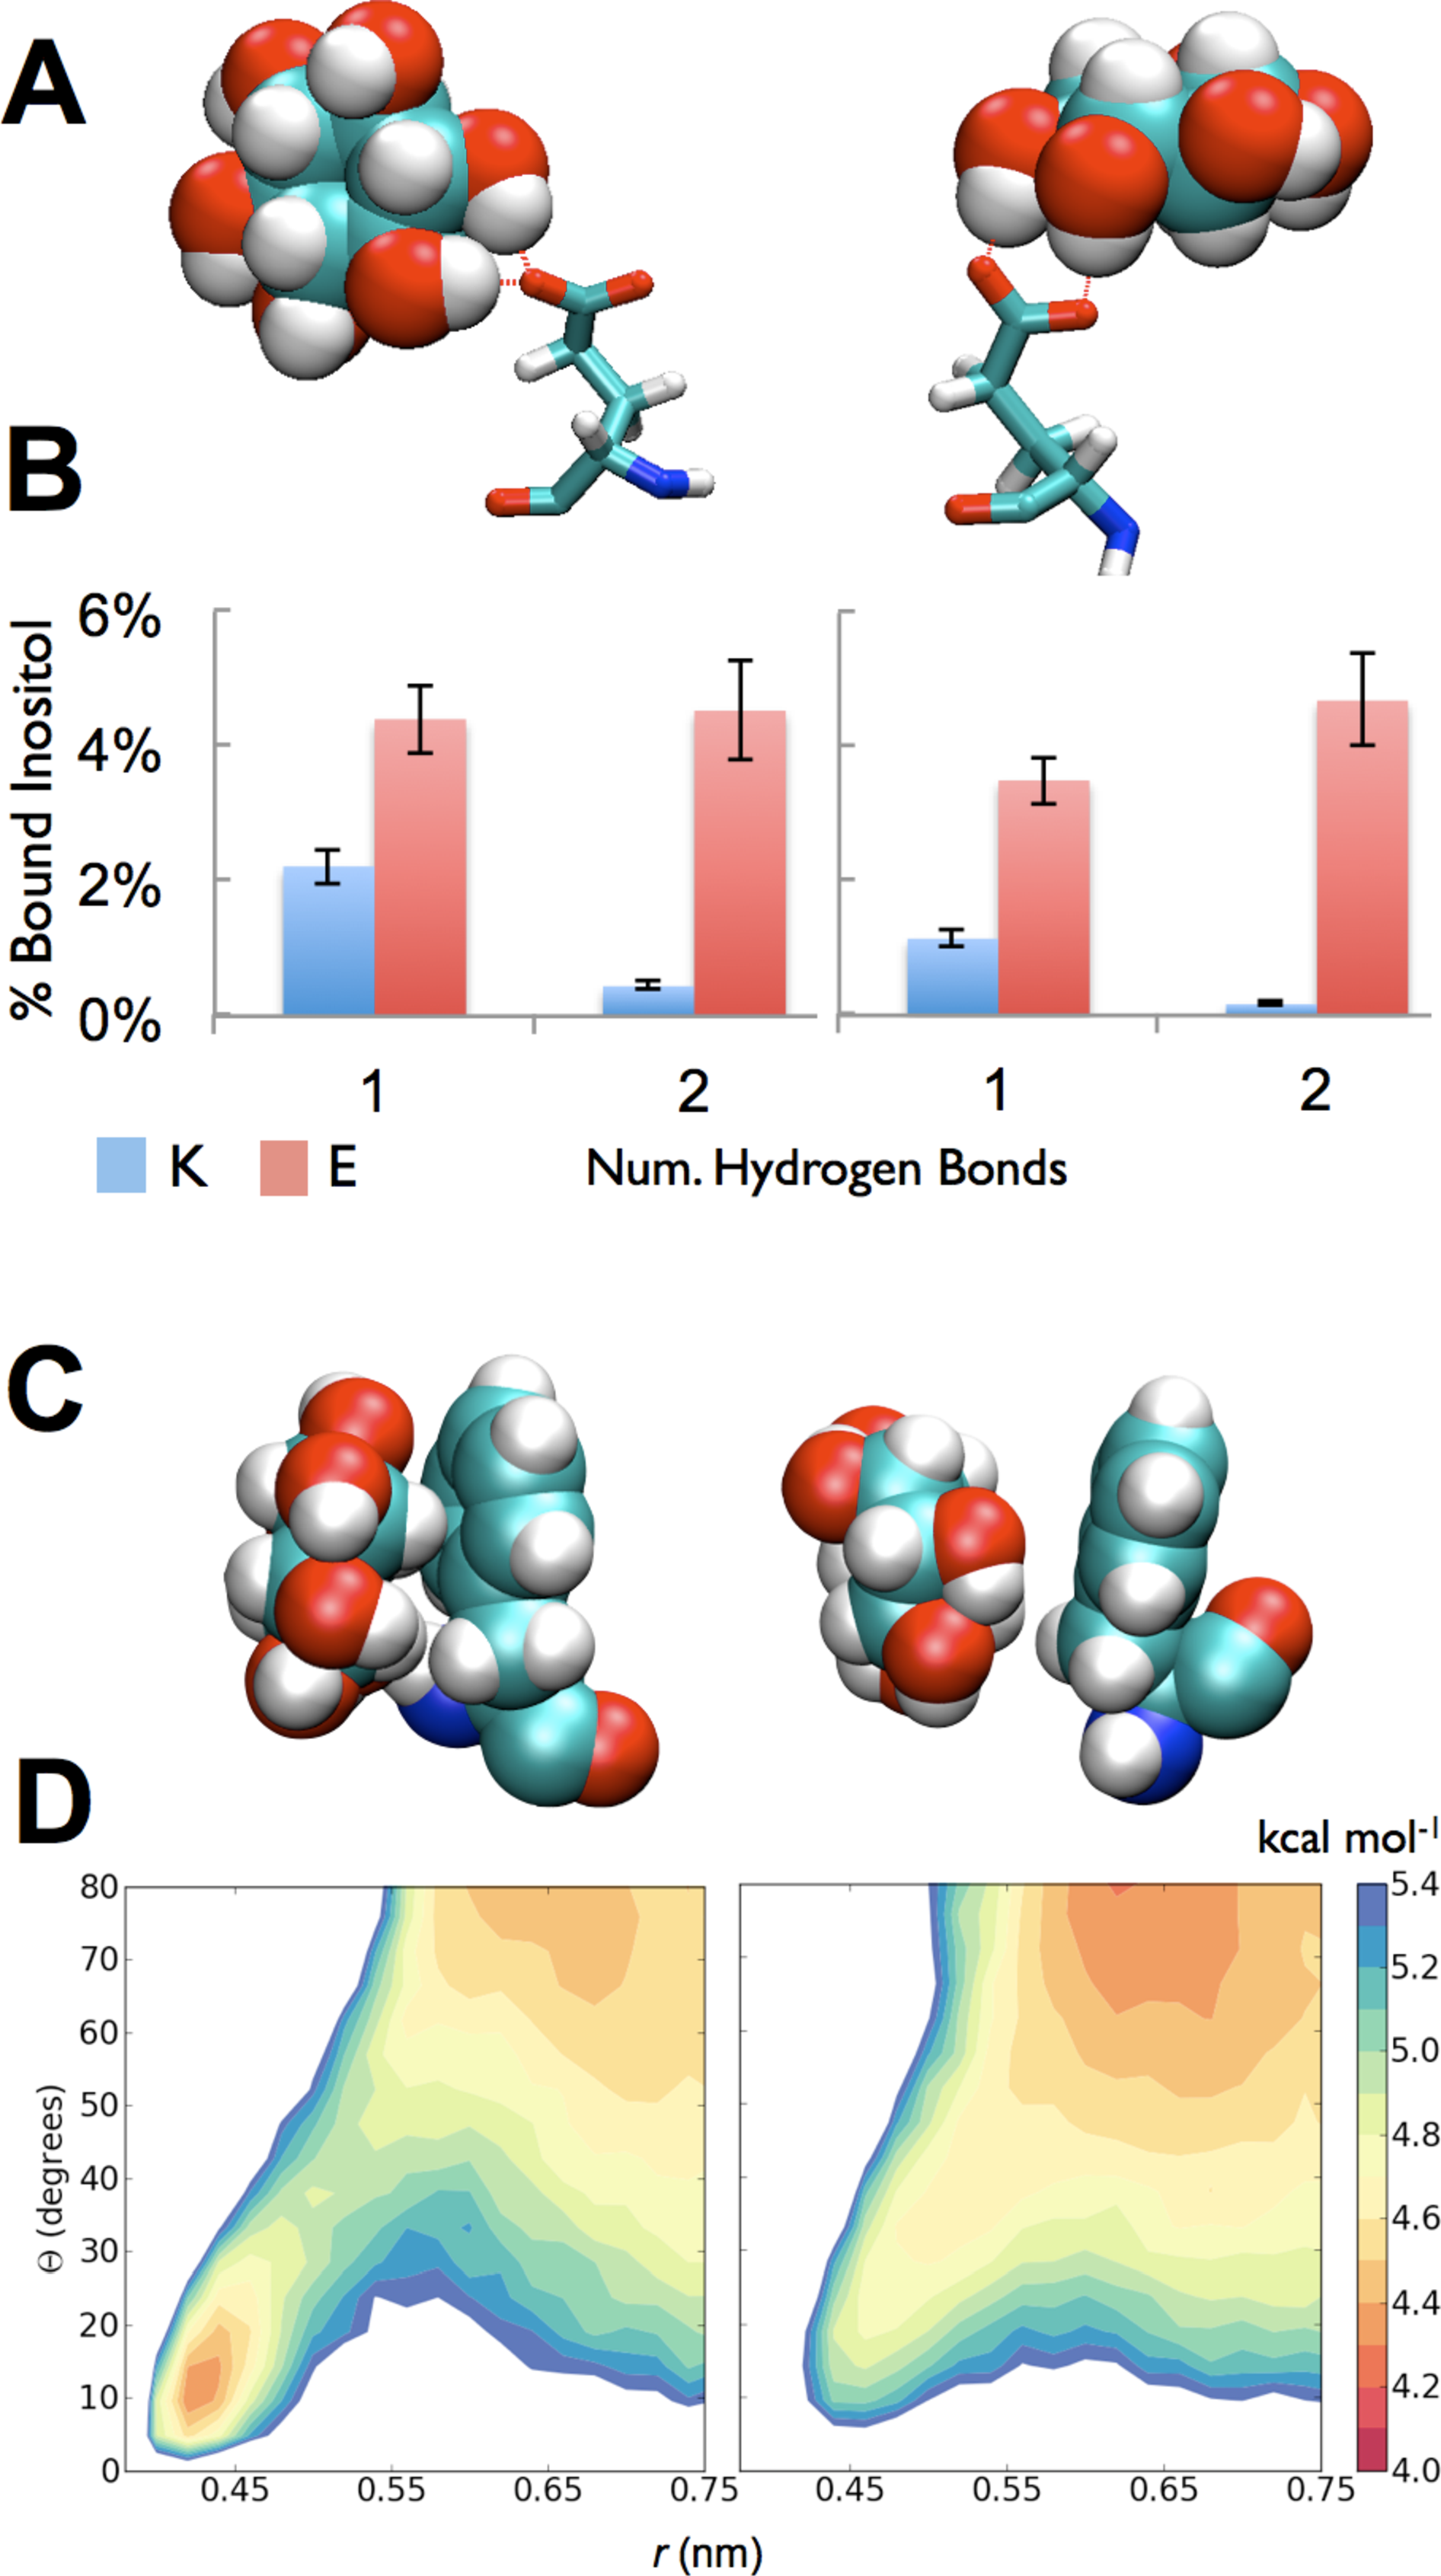
\includegraphics[width=3.185in]{figures/inos2_figures_monomer_residues_pmf_color.pdf}
%\caption{Binding of inositol to Glu and Phe dipeptides. Data for \emph{scyllo}- and \emph{chiro}-inositol are shown on the left and right panels, respectively. (A) Examples of snapshots of inositol bound to the carboxylate group of Glu. (B) Comparisons of the probability of inositol hydrogen bonding to the side chains of Lys and Glu. (C) Examples of nonpolar association between Phe and inositol. (D) Potential of mean force (PMF) of inositol with the phenyl ring of Phe relating $r$, the distance between the centers of geometry of the phenyl and inositol rings, to $\theta$, the planar angle between the rings. Contours are drawn at 0.2 kcal$\cdot$mol$^{-1}$ intervals. Face-to-face stacking for \emph{scyllo}-inositol appears on the PMF at $r=0.45$ nm and $\theta=12\degree$.}
%\label{fig:monomers_glu_phe}
%\end{figure}

%Furthermore, consistent with our previous study of (GA)$_4$, stereochemistry appears to modulate nonpolar binding, but not hydrogen bonding: \emph{scyllo}-inositol was found to bind preferentially to nonpolar groups on phenylalanine and glutamate over the other aliphatic nonpolar residues (Leu, Val and Ala) (Figure~\ref{fig:monomers}E). By contrast, \emph{chiro}-inositol made nonpolar contacts to Phe18, Phe19 and Glu22 with the same probability as with Ala21 (Figure~\ref{fig:monomers}E).

% \sethlcolor{yellow}\hl{Furthermore, of the population of scyllo-inositols bound to Phe via nonpolar contacts, XXX\% of  were bound in the stacked binding mode at a ratio of 15:1, and 7\% at a ratio of 2:1. SHOULD STACKING RESULTS JUST BE MENTIONED IN THE DISCUSSION?}

% I determined the 58% by computing the fraction of all inositols that were stacked divided by the total number of inositols bound to Phe over all frames -- this isn't quite correct because the bound Phes were only counted when the COM (phe, inos) < 0.45 nm
% I need to join this data with the data on the number of nonpolar contacts between phe and inositol

% Note that binding constants similar between low and high molar ratios for monomers once I've switched to the atomic-based contact pairs ... but the difference in kd was more dramatic under the other criteria ... could this mean that there are more stacking interactions at higher molar ratios?
%binding mode of scyllo to the monomer. Given a bound scyllo-inositol molecule to phe (it doesn't really make sense otherwise), it is predominantly bound by XXX, where X\% of time it is  stacking and 100 - X not stacked}.

\subsection{Disordered Oligomer}

To probe the effect of inositol on the early aggregation stages of A$\beta$(16-22), we performed multiple sets of independent MD simulations with four initially disperse A$\beta$(16-22) monomers with inositol:peptide molar ratios of 2:4, 15:4, and 45:4, corresponding to inositol concentrations of 52 mM, 70 mM, and 209 mM, respectively (see Table~\ref{tbl:simulations}). In each of our simulation studies, the peptides spontaneously aggregated with one another over the course of approximately 40 ns, through both hydrogen bonding and nonpolar contacts, to form a disordered oligomer (Figure~\ref{fig:disordered}A). A significant fraction of the residues in the aggregate was in the coil conformation, with only a small fraction of $\beta$-sheet residues occurring in some of the 180-ns simulations (Figure~\ref{fig:disordered}B). Importantly, the distribution of the overall secondary structure of the oligomer was not affected by the presence of inositol, regardless of inositol:peptide molar ratio and inositol concentration (Figure~\ref{fig:disordered}B).

%\begin{figure}
%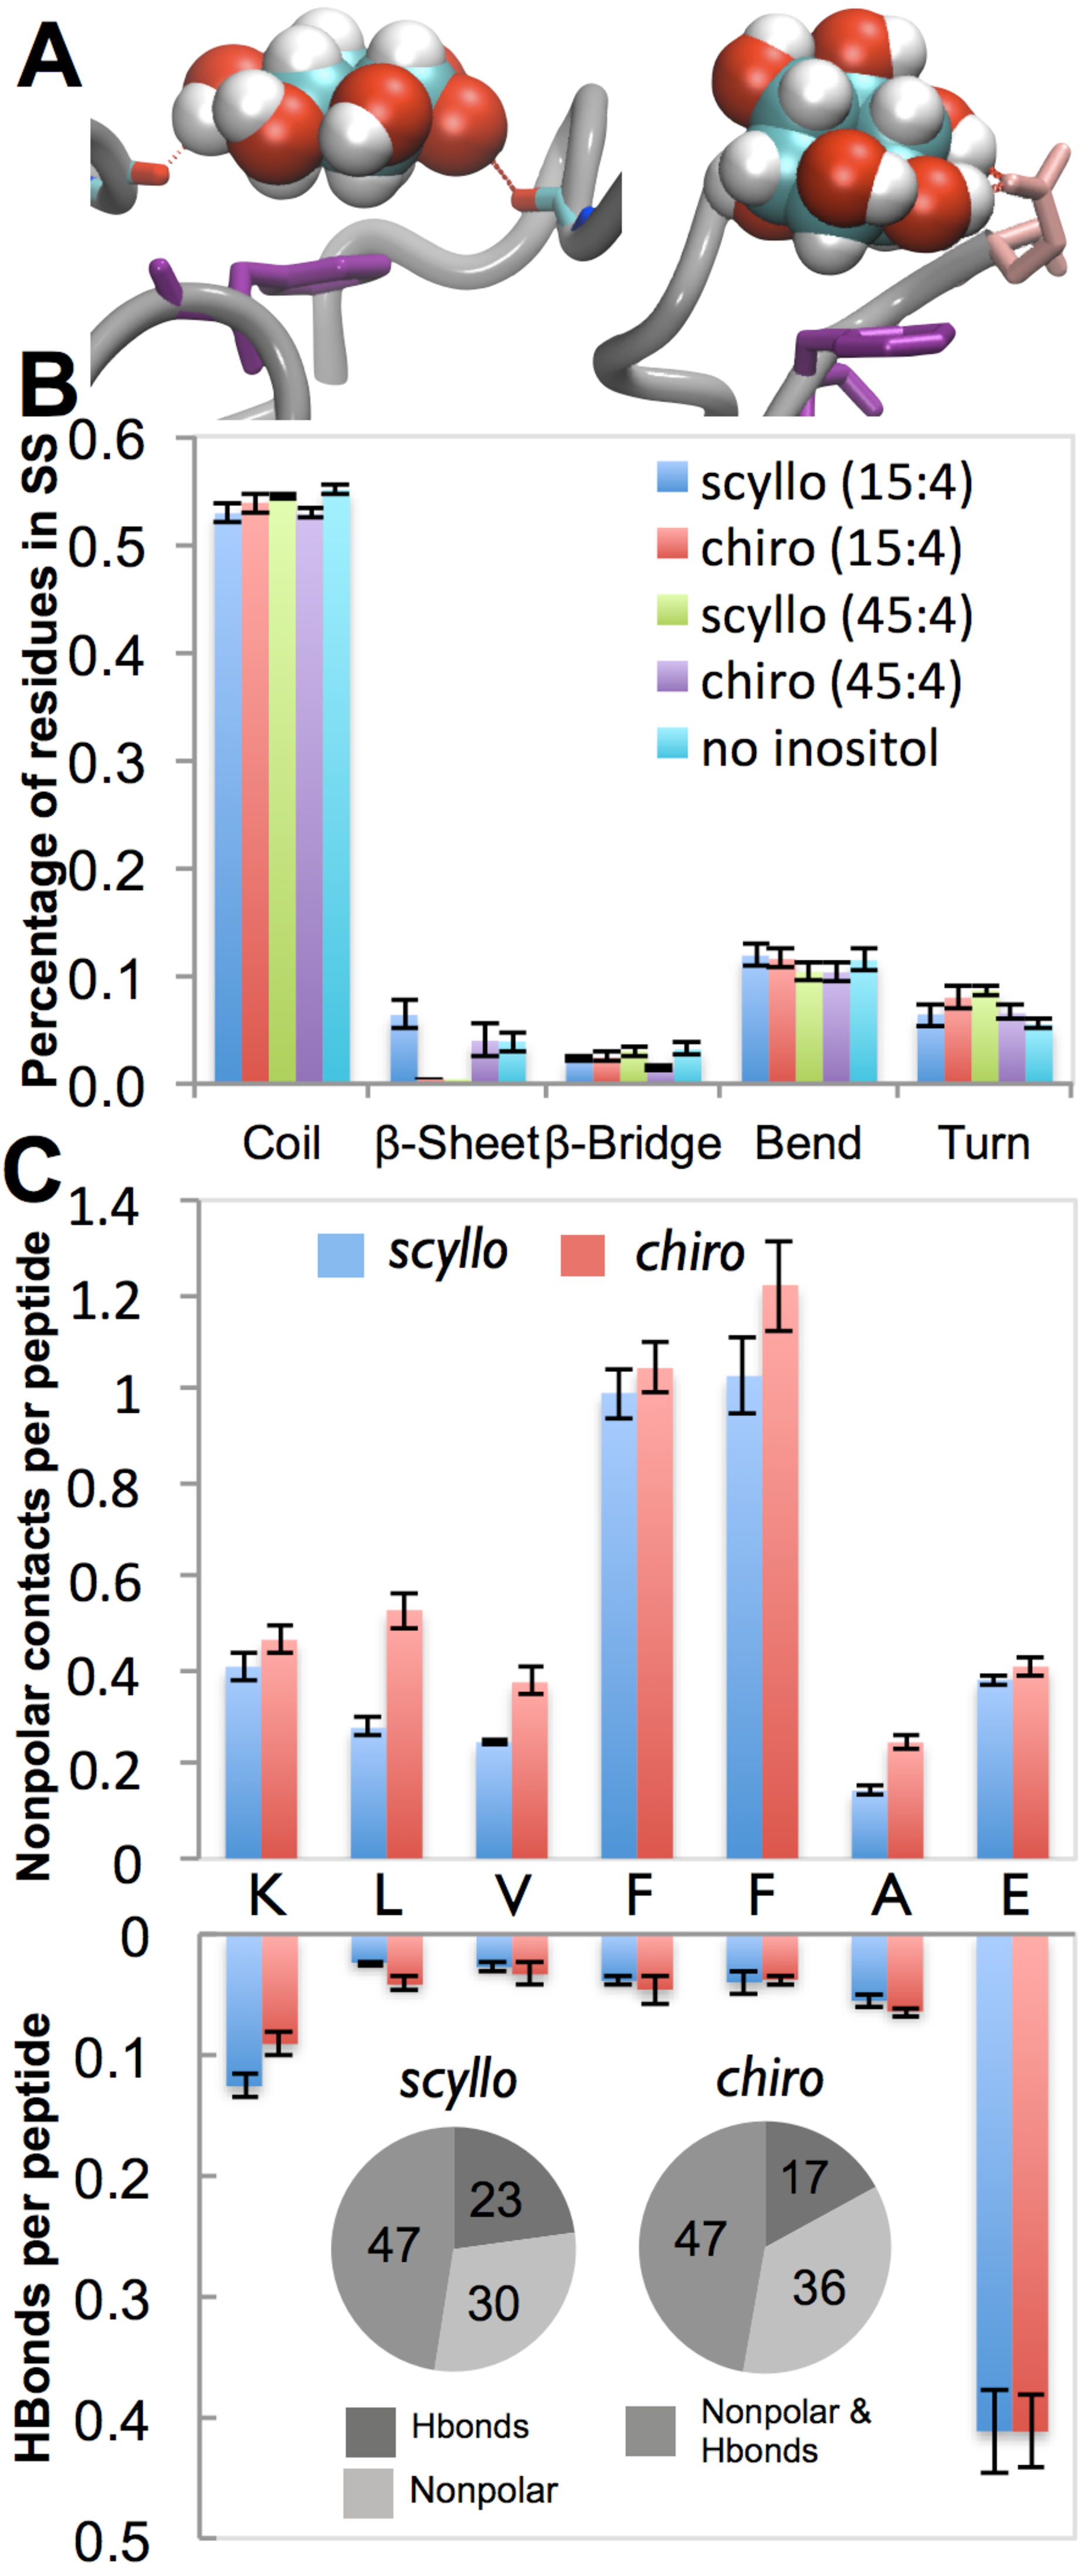
\includegraphics[width=7.96cm]{figures/inos2_figures_disordered_revised.pdf}
%\caption{Binding of inositol to a disordered oligomer of A$\beta$(16-22).  (A) Example snapshots of \emph{scyllo}- (left) and \emph{chiro}-inositol (right) involving both nonpolar contacts and hydrogen bonding. (B) Fraction of residues in the coil, $\beta$-sheet/bridge, bend, and turn as classified by the DSSP algorithm. (C) Time-averaged number of nonpolar contacts (top) and hydrogen bonds (bottom) made by inositol to each residue (per peptide). Inset: Percent of inositol molecules bound to nonpolar and polar groups of the peptide oligomer at an inositol:peptide molar ratio of 45:4 (inositol concentration of 209 mM).}
%\label{fig:disordered}
%\end{figure}

We further characterized the molecular organization of the aggregate by quantifying peptide inter- and intramolecular hydrogen-bonding and nonpolar contacts as measures of the extent of aggregation.  Hydrophobic packing was not affected by the presence of inositol: the equilibrium number of inter-peptide hydrophobic contacts formed per peptide remained approximately 15 regardless of the molar ratio (Figure~\ref{fig:SI-disorderedNumContacts} in the Supporting Information). The average number of intermolecular peptide-peptide hydrogen bonds per chain was approximately the same as the number of intramolecular hydrogen bonds (1.5 vs 1) (Figure~\ref{fig:SI-disorderedNumContacts} in the Supporting Information). Overall, the presence of inositol had no significant effect on the aggregation kinetics or on the morphology of A$\beta$(16-22) oligomers as measured by intermolecular and intramolecular contacts (Figures~\ref{fig:SI-disorderedContactsTS} and \ref{fig:SI-disorderedCluster} in the Supporting Information).

%\begin{table}\footnotesize
%  \vspace{10pt}
%  \caption{Summary of equilibrium constants ($K_{eq}$) for each system in the study.}
%  \label{tbl:bindingConstants}
%  \begin{minipage}{15cm}
%    \renewcommand{\thefootnote}{\thempfootnote}
%    \renewcommand{\footnoterule}{}
%    % \centering
%      \begin{center}
%    \begin{tabular}{| l | *{6}{ c |}}
%       \hline
%         System & Molar ratio\footnote{Inositol:peptide molar ratios} & $scyllo$\footnote{$K_{eq}$ is in units of mM. The standard error is shown within parentheses.} & $chiro$\footnotemark[\value{mpfootnote}] & $1 / N_{peptides}$ & $scyllo$\footnote{Constants in units of mM, estimated by multiplying $K_{eq}$ of monomeric A$\beta$(16-22) (inositol is present at a molar ratio of 15:1) with $1/N_{peptides}$.} & $chiro$\footnotemark[\value{mpfootnote}] \\
%         \hline
%         \hline
%         Monomer & 2:1 & 127 (3) & 104 (1) & 1 & 127 & 104 \\ 
%          	       & 15:1 & 120 (2) & 90 (2) & 1 & 120 & 90 \\ 
%	\hline
%         Disordered oligomer & 2:4 & 28 (4) & 16 (2) & 0.25 & 30 & 23 \\ 
%          			       & 15:4 & 18 (2) & 11(1) & 0.25 & - & - \\ 
%			       	       % For now, comment this out because this wasn't in the previous manuscript
%				       % and I'm not sure how to address this for now. 
%				       & 45:4 & 1.6 (0.4) & 1.9 (0.9) & 0.25 & - & - \\ 
%	\hline
%         $\beta$-oligomer & 4:16 & 15 (2) & 11 (2) & 0.0625 & 8 & 6\\
%         				  & 64:16 &  0.5 (0.3) & 0.18 (0.11) & 0.0625 & - & -\\
%         \hline
%     \end{tabular}   
%  \end{center}
%  \end{minipage}
%  \centering
%  \end{table}

The equilibrium constant ($K_{eq}$) of inositol with the disordered oligomer at molar ratios 2:4 and 15:4 ranged from 10 to 30 mM (see Table~\ref{tbl:bindingConstants}).
% Although these numbers are much smaller than $K_{eq}$ of the monomer, they become comparable when normalized by the number of peptides in the system, $K_{eq}$ (oligomer) $\times$ 4 = 170 mM = $K_{eq}$(monomer), indicating that inositol does not bind small oligomeric aggregates cooperatively. 
% Based on the updated analysis and Keqs -- Binding constants do not indicate cooperative binding at low molar ratios (eg. 2:4 and 2:1), however, at higher molar ratios, a nonlinear decrease in binding constants was observed.  
% I think mention of cooperativity should be entirely moved to the discussion section ...
Similar proportions of bound inositol to nonpolar and polar groups were found at both lower and higher molar ratios (Figure~{\ref{tbl:SI-disorderedBindingMode}} in the Supporting Information). Consistent with our results for the monomer, \emph{chiro}-inositol was more likely than \emph{scyllo}-inositol to bind disordered oligomers exclusively via nonpolar contacts: $\sim$26\% and $\sim$36\% for \emph{scyllo}- and \emph{chiro}-inositol, respectively (Figure~\ref{fig:disordered}C inset and Table~\ref{tbl:SI-disorderedBindingMode}).  
%By contrast, both \emph{scyllo}- and \emph{chiro}-inositol have similar hydrogen bonding propensities (Figure~{\ref{fig:disordered}}C). 
Inversely, \emph{scyllo}-inositol was more likely to bind by hydrogen bonding only ($\sim$23\% vs. $\sim$17\%). Although the number of hydrogen bonds formed along the peptide sequence were independent of inositol concentration (Figure~\ref{fig:disordered}, \ref{fig:SI-disorderedBinding}), the number of nonpolar contacts per peptide approximately doubled upon increasing inositol concentration from 70 to 209 mM.

\subsection{$\beta$-oligomer}

%\begin{figure}
%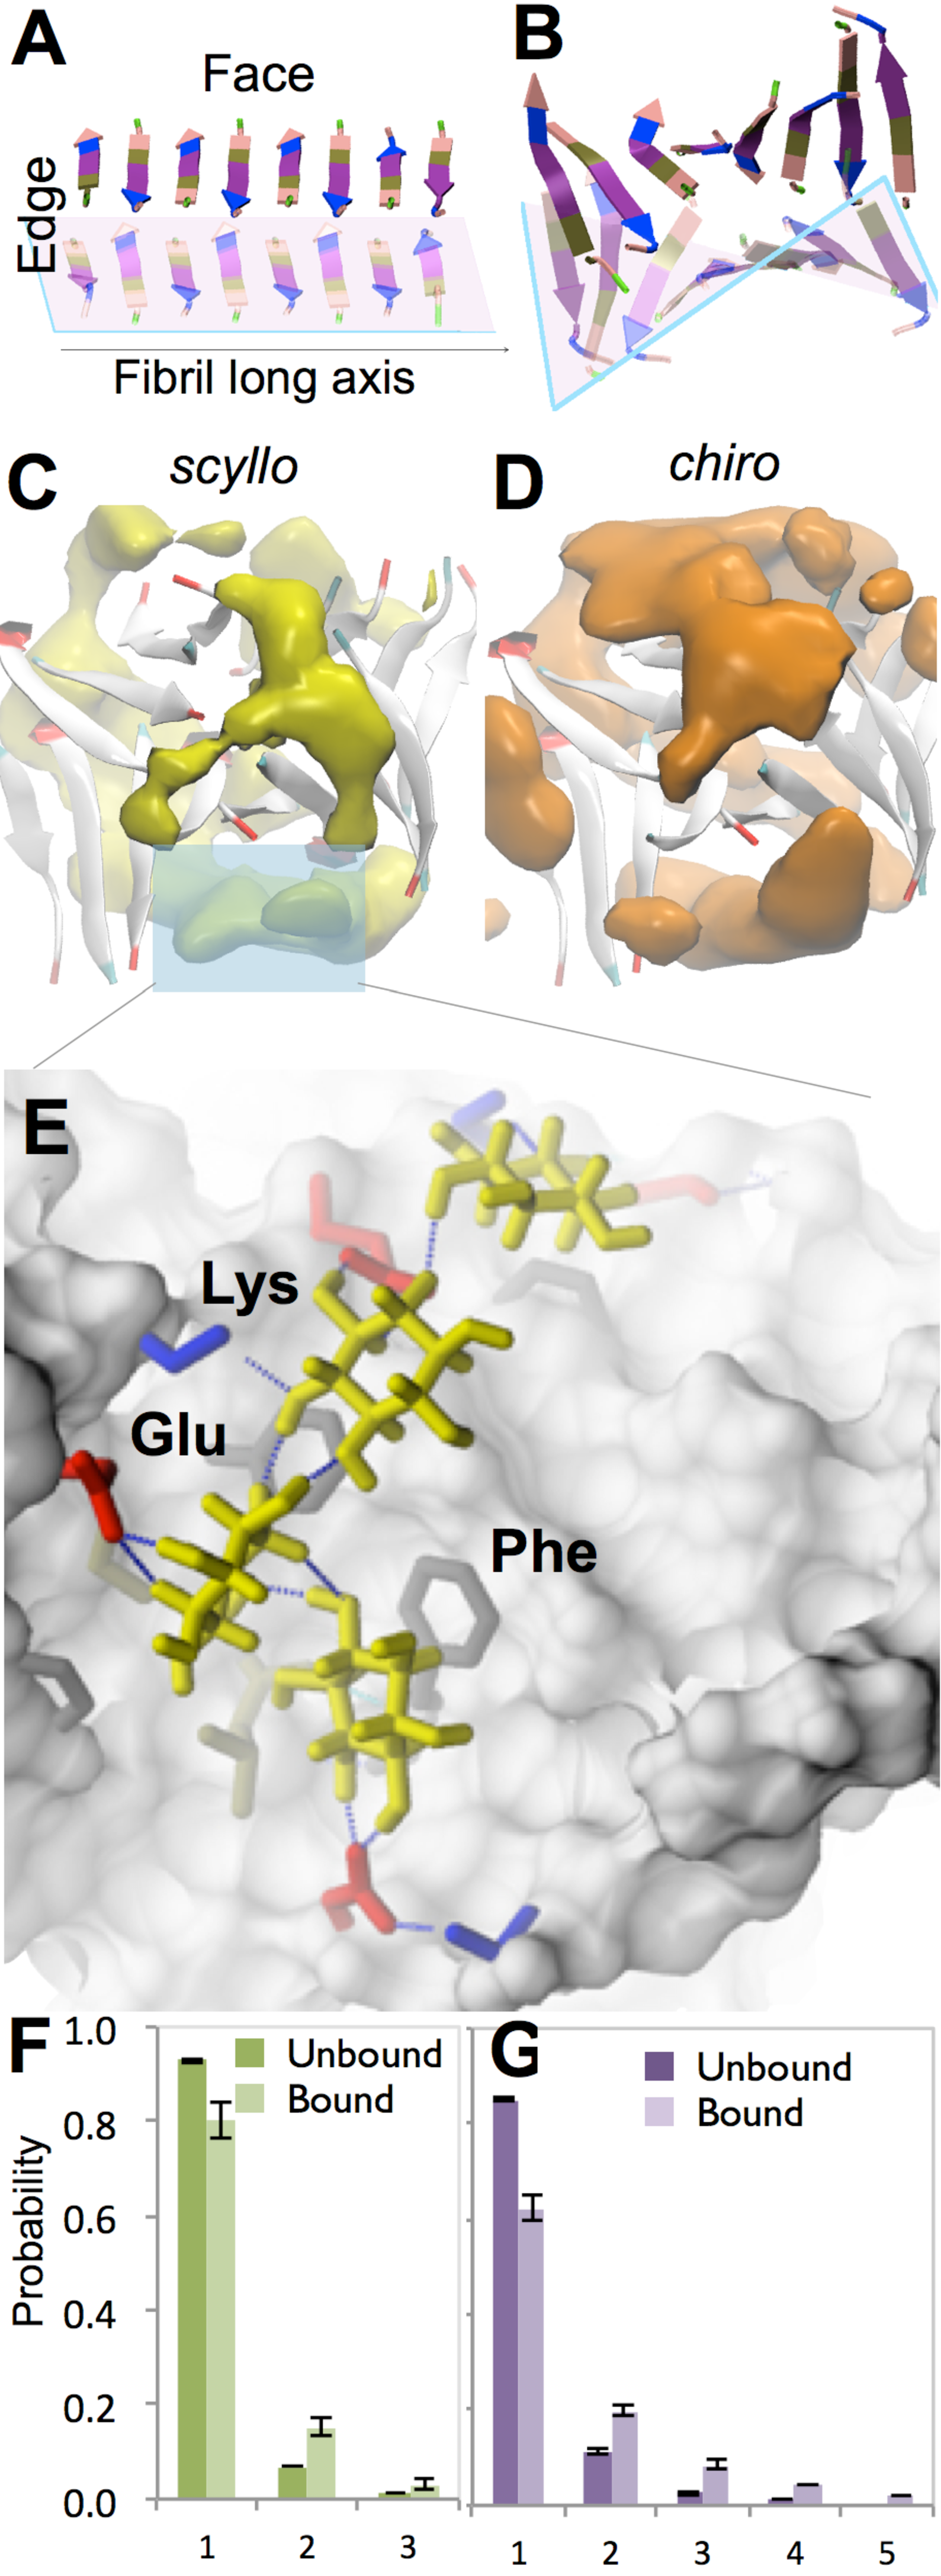
\includegraphics[width=8.1cm]{figures/inos2_figures_beta.pdf}
%\end{figure}
%\begin{figure}[t!]
%\caption{Inositol binding to a $\beta$-oligomer of A$\beta$16-22 (inositol present at a concentration of 208 mM). Schematic depiction of $\beta$-oligomer twisting: (A) the initial rectangular dual-stacked $\beta$-sheet, evolved into (B) a twisted morphology. Spatial probability density maps of (C) \emph{scyllo}-inositol and (D) \emph{chiro}-inositol are shown in yellow and orange, respectively. Surfaces shown correspond to 7\% inositol occupancy. (E) An example of cooperatively-bound \emph{scyllo}-inositol molecules (yellow) at the surface of the $\beta$-oligomer (grey). \hl{Size distribution of bound and unbound clusters of \emph{scyllo}-inositol with the $\beta$-oligomer at inositol concentrations of (F) 62 mM and (G) 208 mM.}}
%\label{fig:beta}
%\end{figure}

Finally, we examine the binding of inositol to an ordered protofibrillar-like aggregate henceforth referred to as the $\beta$-oligomer. In the absence of inositol, rectangularly-stacked sheets (Figures~\ref{fig:SI-betaInitialModel}A-B) spontaneously evolved into a twisted $\beta$-sheet structure with significant inter-strand twisting along the long-axis of the fibril and an inter-sheet twist (Figures~\ref{fig:beta}A-B). The resulting structure has an average inter-strand twist angle of approximately 25$\degree$ for the top sheet and 15$\degree$ for the bottom sheet. Furthermore, the $\beta$-oligomer is comprised of two faces and four edges (Figure~\ref{fig:SI-betaInitialModel}), each of which contains a shallow hydrophobic groove surrounded by polar or charged groups.  In particular, the grooves on the faces are formed by solvent-exposed Phe, Val, and Ala residues and are surrounded on either side by charged side chains of Lys and Glu (Figure~\ref{fig:SI-betaInitialModel}C).

The spatial probability densities of bound inositol depicted in Figures~\ref{fig:beta}C-D show that inositol predominantly binds at the faces of the $\beta$-oligomer. Both stereoisomers have similar affinities with $K_{eq}=$ 15 $\pm$ 2 mM and 11 $\pm$ 2 mM for \emph{scyllo}- and \emph{chiro}-inositol, respectively, at a concentration of 37 mM (inositol:peptide molar ratio of 4:16), and $K_{eq}=$ 0.5 $\pm$ 0.3 mM and 0.18 $\pm$ 0.11 mM at a concentration of 62 mM (molar ratio of 64:16) (Table~\ref{tbl:bindingConstants}).   
% Moving this sentence down to discussion -- Furthermore, $K_{eq}$'s of both stereoisomers decreased significantly (corresponding to an increase in binding) with an increase of inositol:peptide molar ratio, suggesting that the inositols may bind $\beta$-oligomers cooperatively.

% Results that are independent of concentration
% Also note that I'm stating the results without qualifying the molar ratio or concentration ... I should have a statement either saying they are the same at first, then stating the specifics.
Consistent with the binding densities depicted in Figure~\ref{fig:beta}, inositol molecules display the highest binding propensity to the nonpolar groups of Phe and Lys and the charged groups of Lys and Glu, all of which are located on the faces of the $\beta$-oligomer (Figure~\ref{fig:SI-betaInitialModel}C). Inositol molecules did not penetrate the $\beta$-sheet core of the oligomer: the fraction of hydrogen bonds to each residue depicted in Figure~\ref{fig:beta_residue_binding} (bottom panel) show that, relative to side chains, little or no hydrogen bonds were made with the backbone of residues Leu, Val, Phe, and Ala. Although inositol molecules sometimes intercalated between $\beta$-strands, these rare events did not lead to the disaggregation of the preformed $\beta$-oligomer in any of our simulations.

%\begin{figure}
%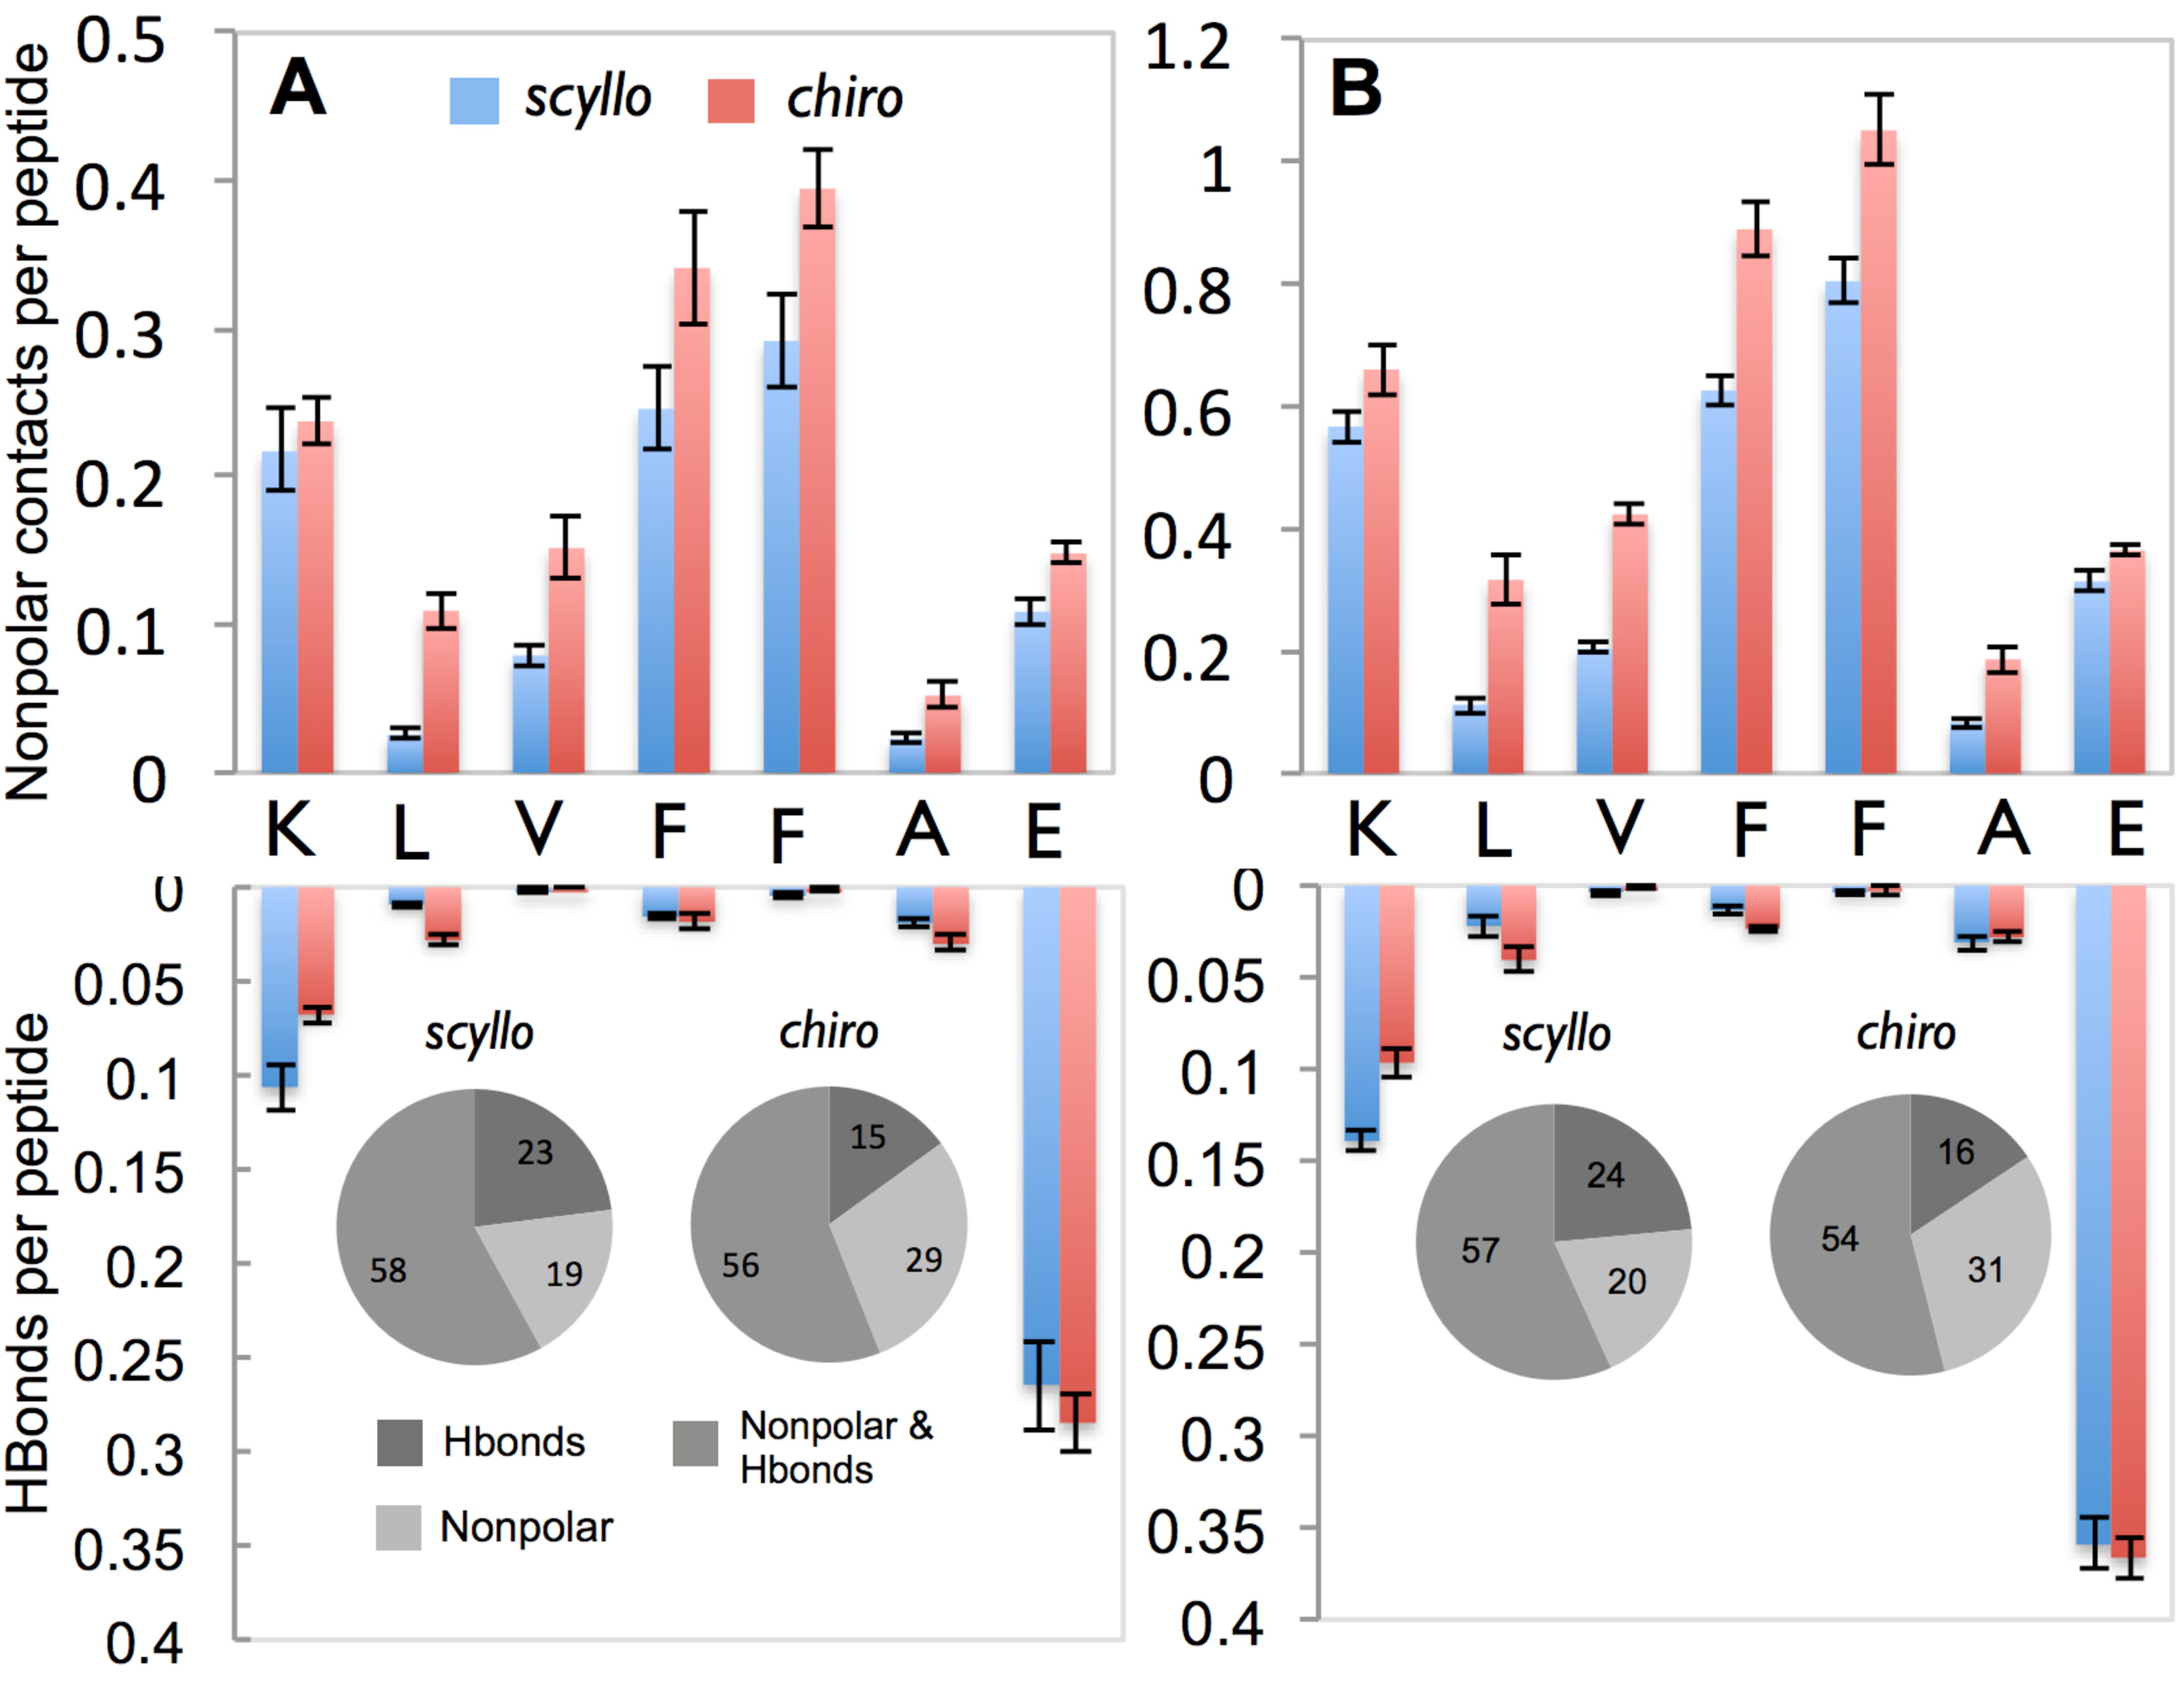
\includegraphics[width=15cm]{figures/inos2_figures_beta_residues_revised.pdf}
%\caption{Binding propensity of inositol to nonpolar and polar groups on the $\beta$-oligomer. Time-averaged number of nonpolar (top) and hydrogen bonds (bottom), per peptide, made by inositol to each residue of the $\beta$-oligomer. Inset: Percent of \emph{scyllo}- and \emph{chiro}-inositol molecules bound to nonpolar and polar groups of the $\beta$-oligomer.  Inositol is present at a concentration of 62 mM in (A) and 208 mM in (B).}
%\label{fig:beta_residue_binding}
%\end{figure}

Independently of inositol concentration, a higher fraction of \emph{scyllo}-inositol than \emph{chiro}-inositol formed hydrogen bonds with the $\beta$-oligomer (inset of Figure~\ref{fig:beta_residue_binding} and Table~\ref{tbl:SI-betaBindingMode}):  $\sim$23\% versus $\sim$15\%, respectively. Concomitantly, the fraction of \emph{chiro}-inositol molecules forming nonpolar contacts ($\sim$29\%) was higher than that of \emph{scyllo}-inositol ($\sim$19\%) (inset of Figure~\ref{fig:beta_residue_binding} and Table~\ref{tbl:SI-betaBindingMode}).

% Results which are modulated by concentration
% \sethlcolor{green}
At the higher inositol:peptide molar ratio of 64:16, bound inositol molecules were significantly more likely to be clustered than free inositol: 20\% versus 8\% (Figure~{\ref{fig:beta}}F-G) at 62 mM. Moreover, the size of bound clusters increased with concentration. Inositol molecules within a cluster were usually hydrogen bonded 
% this may not be right because they can form nonpolar contacts too
to each other via their free hydroxyl groups, while simultaneously forming hydrogen bonds and/or nonpolar contacts with the peptide.  Such a binding mode is depicted in Figure~{\ref{fig:beta}}E, where a hydrogen-bonded chain of four  \emph{scyllo}-inositol molecules occupies a shallow groove on the $\beta$-oligomer surface. % [Add additional examples of clustered binding to SI for both scyllo and chiro and reference them here]
There was no difference in distribution of cluster size between \emph{chiro}- and \emph{scyllo}-inositol.

Furthermore, the binding propensity of \emph{scyllo}- and \emph{chiro}-inositol for hydrophobic groups increased with inositol concentration (Figure~\ref{fig:beta_residue_binding}).  At lower concentrations ($\sim$30 - 60 mM), both nonpolar and hydrogen bonding propensities increased with molar ratio, suggesting that single molecules and dimers of inositol have similar binding propensities, and binding to the protofibril involves forming both nonpolar contacts and hydrogen bonds.  However, at a concentration of 208 mM, the nonpolar binding propensity of inositol increased whereas the hydrogen bonding propensity remained the same.  As a result, inositol molecules in large clusters (of size three or more) form, on average, more nonpolar contacts with the $\beta$-oligomer than their singly-bound counterparts.
% \sethlcolor{yellow}
% I took out cooperative binding modes in the description of Figure 4E because that is implying that there is cooperativity without any evidence -- this speculate/extrapolation will be left to the discussion section.

% Move the comparisons of this is modulated by stereochemistry and aggregate morphology.
% This is a result not previously observed for the monomer and disordered oligomer of A$\beta$(16-22).

% TODO ADD/Find EVIDENCE FOR KLVFFAE IMPORTANT FOR STACKING -- I could be just bullshitting here, in any case, stacking interface mediated by KLVFFAE is not the only reason why binding to this segment is useful .. LVFFA is also at the fibril core .. disrupting packing here disrupts amyloid formation of Abeta42].  \cite{Takeda:2009es} -- Caflish and Derreumaux computation evidence that 12-22 is the "aggregation interface"

% TODO Look into this further: My results are exactly consistent with the mechanism proposed by Porat for polyphenol inhibition! planar + equatorial OHs => target amyloidgenic core! Except I have data to prove it. EGCG, an effective inhibitor of Abeta42 amyloid formation, has this structure and was shown to bind fibrillar forms of Abeta42.\cite{Bieschke:2010ju}

\section{Discussion}
In the above analysis, we have systematically characterized the binding of \emph{scyllo}-inositol and its inactive stereoisomer, \emph{chiro}-inositol, with monomer and aggregates of A$\beta$(16-22). Below, we consider the implications of our findings for the activity of inositol in the A$\beta$42 amyloid aggregation pathway.

\subsection{Comparison of inositol binding to monomers and aggregates of A$\beta$(16-22)}
Consistent with our results on the binding equilibrium of inositol with model amyloidogenic peptides,\cite{Li:2012p853} both \emph{scyllo}- and \emph{chiro}-inositol bound weakly, and with similar binding constants, to the monomeric and aggregated states of A$\beta$(16-22) considered. % Should I leave this extrapolation to full-length A$\beta$ ?
However, the equilibrium constants ($K_{eq}$) computed in this study are about an order of magnitude smaller than those obtained in our previous study, namely, in the range of 0.2 - 120 mM for A$\beta$(16-22) versus 40 - 1000 mM for a model peptide of similar length, $(GA)_4$.\cite{Li:2012p853} Because all observed binding sites and modes are accounted for in the calculation of $K_{eq}$ in our study, this quantity should be interpreted as an estimate of the binding avidity rather than the binding affinity of inositol.  This decrease in $K_{eq}$, and hence, an increase in binding avidity, is due to the presence of sequence-specific binding sites and modes in A$\beta(16-22)$.

Both \emph{scyllo}- and \emph{chiro}-inositol bound most weakly to monomers, with $K_{eq}=$ 120 $\pm$ 2 mM and 90 $\pm$ 2 mM, respectively, at the highest molar ratio (Table~\ref{tbl:bindingConstants}). Because inositol binding to the peptide monomer is not cooperative, a predicted $K_{eq}$ of monomeric A$\beta$42 can be obtained by linearly scaling the $K_{eq}$ of inositol for monomeric A$\beta$(16-22) with the ratio of peptide lengths of A$\beta$(16-22) to A$\beta$(1-42).  On the basis of the value of $K_{eq}$ of inositol at the highest molar ratio, this value would be 120 mM/6 = 20 mM, which is an order of magnitude higher than the concentration (1 mM) at which inhibition was observed \emph{in vitro}.\cite{McLaurin:2000p64}  Moreover, our results indicate that the conformational equilibrium of monomeric A$\beta$(16-22) is not displaced in the presence of inositol (Figure~\ref{fig:monomers}A). Taken together, these results suggest that inositol is unlikely to act as a drug by binding to and displacing the conformational equilibrium of monomers of A$\beta$42.

Likewise, inositol bound only weakly to small disordered oligomers, with $K_{eq}$ $\sim$10 - 30 mM at a concentration of 70 mM for both \emph{scyllo}- and \emph{chiro}-inositol (Table~\ref{tbl:bindingConstants}). Independently of the presence of inositol,  A$\beta$(16-22) peptides formed amorphous aggregates with only a small amount of secondary structure. These aggregates predominantly involved intermolecular nonpolar contacts (Figure~\ref{fig:SI-disorderedContactsTS}), indicating that hydrophobic association is the primary driving force for the self-assembly of A$\beta$(16-22) peptides in solution. Inositol molecules were found to bind both monomers and small oligomers of A$\beta$(16-22) predominantly via nonpolar interactions (Figures~{\ref{fig:monomers}} and {\ref{fig:disordered}}),  suggesting that they may disrupt the hydrophobic association of nonpolar groups. However, due to weak binding, we speculate that inositol is unlikely to prevent early oligomer formation in the A$\beta$42 fibrillation pathway by binding to A$\beta$(16-22).

% TO A DEGREE THERE IS SOME COOPERATIVITY FOR DISORDERED OLIGOMERS TOO (that is 30 versus 20 mM, where the difference is within error bars).
In contrast, inositol displays a much higher binding avidity for $\beta$-oligomers, with $K_{eq}=$ 0.5 $\pm$ 0.3 mM and  0.18 $\pm$ 0.11 mM for \emph{scyllo}- and \emph{chiro}-inositol (at a concentration of 62 mM), respectively. Notably, these $K_{eq}$ values are in quantitative agreement with experimental concentrations (0.5 - 1 mM) sufficient for the inhibition of A$\beta$42 fibrillation \emph{in vitro},\cite{McLaurin:2000p64} suggesting that $\beta$-oligomers may be an \emph{in vitro} binding partner of inositol.

% Difference in the binding modes between the inositol stereoisomers
A key finding of this study is that the stereospecificity of binding by inositol stereoisomers is not due to different $K_{eq}$'s, but rather to different binding modes with nonpolar groups of side chains with specific geometries. In particular, due to the presence of planar hydrophobic faces, \emph{scyllo}-inositol, unlike \emph{chiro}-inositol, can bind Phe side chains (or other side chains with planar geometries) in a planar face-to-face stacking mode (Figure~\ref{fig:monomers_glu_phe}D). In all of our systems considered, this stacking mode accounts for $\sim$9\% of Phe bound by \emph{scyllo}-inositol, and increases to about 10 - 12\% at higher concentrations of \emph{scyllo}-inositol.

% \hl{Although \emph{scyllo}- is able to adopt specific binding modes, \emph{chiro}-inositol has a greater propensity than \emph{scyllo}-inositol to bind to nonpolar groups of A$\beta$(16-22) independently of aggregate morphology (Figures~{\ref{fig:monomers}}, {\ref{fig:disordered}}, {\ref{fig:beta_residue_binding}}). 

Furthermore, the binding probability densities of \emph{scyllo}-inositol are more localized to the grooves of $\beta$-oligomers, whereas those of \emph{chiro}- are spread more widely (Figure~{\ref{fig:beta}}). This difference in spatial distribution is consistent with the difference in binding avidity, which was higher for \emph{chiro}-inositol than for \emph{scyllo}-inositol in all of the systems considered. Moreover, \emph{scyllo}-inositol displays a higher hydrogen-bonding propensity than \emph{chiro}-inositol, which is likely to contribute to its higher binding specificity. % should I say hydrophilic here? I don't really call them hydrophilic elsewhere 
Taken together, our results suggest that \emph{scyllo}-inositol binds with more specificity than \emph{chiro}-inositol to $\beta$-sheet aggregates of A$\beta$(16-22).

Furthermore, binding modes of inositol involving nonpolar groups are modulated by aggregate morphology: the change in morphology from monomers to oligomers resulted in a significant decrease in the population of stereoisomers bound exclusively by nonpolar contacts, concomitant with an increase in the population of stereoisomers forming both nonpolar contacts and hydrogen bonds with the peptides. This difference is more pronounced for the $\beta$-oligomer (Figure~{\ref{fig:beta_residue_binding}}). Our results indicate that both hydrogen bonding and nonpolar interactions are important for the binding of inositol to A$\beta$(16-22), and that the balance of these interactions is modulated by both aggregate morphology and inhibitor stereochemistry.
%We speculate that both of these interactions may play a key role in the binding mechanism of small-molecule amyloid inhibitors in general.

\subsection{Binding cooperativity with $\beta$-oligomers}

The binding avidity of both \emph{scyllo-} and \emph{chiro}-inositol decreased significantly (corresponding to an increase in binding) with an increase of inositol:peptide molar ratio: $K_{eq}=$ 10 - 15 mM and 0.1 - 0.5 mM at 4:16 and 64:16 molar ratios, respectively.  This finding is consistent with the existence of cooperative binding involving clusters of multiple inositol molecules at higher molar ratios (Figure~{\ref{fig:beta}}E). Here we refer to cooperative binding as the propensity of ligand binding at one or more sites to increase the affinity for the binding of additional ligands at other sites. Furthermore, the size of these clusters is modulated by inositol concentration (Figure~{\ref{fig:beta}}F-G). Taken together, our results suggest that inositol binding is cooperative at sufficiently high molar ratios and concentrations. In support of our findings, a recent combined simulation and biophysical study on the polyphenolic inhibitor EGCG indicated that binding modes of other small-molecule inhibitors may be modulated by ligand:peptide molar ratio:  an increase of EGCG:A$\beta$42 molar ratio shifted the predominant binding interaction of EGCG from hydrogen-bonding to hydrophobic interactions.\cite{Wang:2010p204}

% By binding to the surface of the $\beta$-oligomer, inositol molecules may alter its characteristics to promote the binding of additional inositol molecules, which may bind at adjacent sites by forming hydrogen bonds and nonpolar contacts with pre-existing inositols and the protein.
% The increase in the binding affinity of additional inositols, despite a decrease in the number of possible binding sites, is likely due to pre-existing bound inositols, which by exposing hydrogen bonding groups in proximity to nonpolar groups of the protein may form binding sites that favorable for binding. 

Our results suggest that the binding cooperativity of inositol results from a combination of favorable intermolecular interactions with peptide and inositol groups: by exposing multiple hydrogen bonding groups in proximity to nonpolar groups of the protein, bound inositol molecules promote the binding of additional inositol molecules at adjacent binding sites.
% Accordingly, inositol predominantly binds with the $\beta$-oligomer by forming both nonpolar contacts and hydrogen bonds, suggesting that inositol molecules preferentially bind at sites where both types of interactions may be satisfied} (Figure~{\ref{fig:beta_residue_binding}}).
% This paragraph is basically a description of the receptor multivalency ... which is also important for achieving cooperative binding in this case (should make an explicit statement ... our data suggests this)
By contrast, a linear dependence of binding avidity upon inositol concentration was observed for the monomers and the disordered oligomers (Table~{\ref{tbl:bindingConstants}}), presumably because these morphologies cannot accommodate this type of multivalent interaction.
 
The increase in the binding avidity of inositol for the $\beta$-oligomer of A$\beta$(16-22) relative to monomeric and disordered oligomeric forms may be explained by structural features present in the former, but not in the latter species. First, the $\beta$-oligomer has a much larger effective surface area, which can accommodate multiple bound inositol molecules (Figure~{\ref{fig:beta}}E). Second, as a direct consequence of its morphology,  the $\beta$-oligomer presents grooves on its surface that collocate the residues (i.e. Phe and Glu) capable of high-affinity interactions with inositol. 

Taken together, these findings suggest that the clustering of inositol molecules may be important for increasing the local concentration of inositol in the vicinity of the peptide, and could play a role in overcoming the weak binding affinity of individual inositol molecules in order to achieve drug-like activity. Similarly, recent simulation studies of A$\beta$40 fibrillar fragments and non-steroidal anti-inflammatory drugs, ibuprofen and naproxen, suggested that their inhibitory activities may be related to their ability to bind cooperatively and to form clusters on the surface of A$\beta$40 fibrillar aggregates.\cite{Takeda:2010p34,Raman:2009p47}

% Interestingly, although the binding avidity of inositol increased with molar ratio, the binding modes and propensities of inositol remained the same, suggesting that inositol adopts high avidity binding modes in sites where nonpolar and charged residues are in close proximity to each other.  [Note that I think I should remove the above sentence ... as it is neither informative nor ``true'' (because propensities don't remain the same with increased molar ratio. Nor do binding modes -- with increased molar ratio (more of inositol), you get clustering ... which is a different binding mode.) ... and turn the sentences  below to support my results ... that at higher molar ratio / concentration .. binding modes may change -- as in our case, there was clustering.]
% Note that NP binding propensity also increases for the disordered oligomers, but I haven't really addressed that here.

% What is the increase in molar ratio, what is the relative increase in nonpolar binding propensities? -- look at the supplementary information (The relative increase in nonpolar contacts is much less than in the increase in molar ratio) -- why does this matter?


\subsection{Proposed mechanism of A$\beta$ amyloid inhibition}

Mature amyloid fibrils are thought to form either by $\beta$-strand addition along the long axis of the fiber (elongation) or by lateral face-to-face association with other protofibrils.\cite{Straub:2011p174} It follows that small molecules that can disrupt either of these interactions may inhibit fibrillation. In addition, multiple experimental studies have shown that A$\beta$(16-22) is part of the $\beta$-sheet core of fibrils of A$\beta$42\cite{Hilbich:1992vy,Gordon:2001tj,Watanabe:2002ti,Inouye:1993ku,Paravastu:2009fi} and is central to the fibrillation of A$\beta$40/42.\cite{Cukalevski:2012ks, deGroot:2006p4453} 
Furthermore, the structures of several fibril polymorphs suggest that residues 16-22 mediate the stacking of constituent protofilaments in mature fibrils.\cite{Petkova:2002p192,Luhrs:2005p229,Paravastu:2009fi,Wu:2010p3553} Consistent with these observations, the fibrillar structure of full-length A$\beta$42 from a solid-state NMR study shows that the protofibril has two different $\beta$-sheet faces, one of which is formed by the A$\beta$(17-22) peptide segment.\cite{Luhrs:2005p229}

% This is another reference I might add in support of KLVFFAE \cite{Senguen:2011hz}
% Note need to tie together the last three pieces together a bit more. The drive home point is that the affinity + cooperativity + binding in grooves to glutamate & F => binding is exactly carbohydrate like, and this is the most likely binding site for inositol.
% Stereochemistry modulate binding specificities of sugar molecules - need examples

Our results suggest that A$\beta$(16-22), the peptide sequence forming the fibrillar core of full-length A$\beta$42, is a likely binding site for inositol. Furthermore, our results indicate that \emph{scyllo}-inositol binds to this region more specifically than \emph{chiro}-inositol. We hypothesize that \emph{scyllo}-inositol, by binding to and coating the $\beta$-sheet surfaces of protofibrils involving A$\beta$(16-22), disrupts the lateral stacking of these oligomers, which ultimately leads to the inhibition of fibril formation. Consistent with this hypothesis, the amyloid dye Congo red has been suggested by previous studies to disrupt amyloid formation in a similar manner - i.e. by binding to grooves on the surface of extended $\beta$-sheets.\cite{Shea:2012eh,Wu:2007p361}

Furthermore, based on our results, we hypothesize that planar nonpolar faces with multiple hydroxyl groups in equatorial positions around the ring confer binding specificity to small molecules for the amyloidogenic core of A$\beta$, and thus are key features for their activity. Consistent with this hypothesis, \emph{in vitro} studies of small-molecule derivatives of \emph{scyllo}-inositol showed that the substitution of a single hydroxyl by a ketone group resulted in loss of activity (i.e., fibrils were formed).\cite{Nitz:2008p13,Sun:2008p208,McLaurin:2000p64} Moreover, polyphenols, many of which are strong \emph{in vitro} inhibitors of amyloid formation, all possess planar nonpolar faces with hydroxyl groups arranged equatorially. A similar hypothesis was recently put forth based on structure-activity relationships of polyphenols as a possible explanation for their effectiveness in inhibiting amyloid formation. \cite{Porat:2006p33}
% Add or refine the above? Speculation - perhaps hydrogen bonding interactions are equally important as hydrophobic interactions in small molecule amyloid inhibition. Perhaps need a balance of both? Interestingly, a change in 2 equatorial hydroxyl groups to 2 axial groups (when going from scyllo form to the chiro form) led to a significant decrease in the likelihood to form hydrogen bonding interactions in chiro-inositol.

Many differences exist between the $\beta$-oligomer of A$\beta$(16-22) and protofibrils of the full-length A$\beta$ peptides. Our results indicate that inositol binding depends on both the fibrillar morphology and the surface physico-chemical properties of the peptide aggregate. % Is this still true?  Binding propensities are the same for all systems.  Only the binding avidities are different.  Binding modes are somewhat different between monomers and oligomers, but they are fairly similar between disordered and beta, with the exception of a decrease in the nonpolar population and an increase in the nonpolar & polar population - this means that there is a binding mode different modulated by morphology -- so this statement is still true.  Question: What fraction of the nonpolar and polar binding mode consists of nonpolar stacking + hbonding?
Thus, alternative binding modes and binding sites of inositol may exist on aggregate forms of the full-length A$\beta$42 peptide, which cannot be deduced from the results of this study. As part of our future directions, we will perform comparative simulation studies of \emph{scyllo}- and \emph{chiro}-inositol binding to aggregates of full-length A$\beta$.

\subsection{Similarity to Carbohydrate Binding}

	A striking result of our study is the characteristic sugar-like\cite{Taroni:2000uh} binding affinities and binding modes of inositol. Similar to inositol, monosaccharides exhibit millimolar binding affinities for lectins, a class of sugar-binding proteins.\cite{Schnupf:2010p6654,Geisler:2010p188} Furthermore, sugar binding usually involves a combination of hydrogen bonds between hydroxyl groups and charged side chains (Asp or Glu) and nonpolar stacking of aromatic moieties, which are important for the recognition and selectivity of sugar enantiomers by lectins.\cite{Sharon:2001p215}. Consistent with these observations, our results indicate that inositol displays higher binding propensities to Phe and Glu compared to Lys, Leu, Val, and Ala. Moreover, from our simulations, the binding free energy of stacking to the phenyl ring of Phe is approximately -0.5 kcal/mol,  in agreement with that of glucose binding to the indole group of tryptophan obtained from recent MD simulation\cite{Schnupf:2010p6654} and NMR studies\cite{Kiehna:2007p163}. 
	Finally, the shallow amphiphilic grooves found at the surface of $\beta$-oligomers (Figure~\ref{fig:beta}E) are analogous to binding sites located at the surface of carbohydrate-binding domains.\cite{Taroni:2000uh,Kulharia:2009p212,Weis:1996p225} Akin to the multivalency in binding often exhibited by carbohydrates,\mbox{\cite{Lee:1995ul}} by forming multiple weak affinity interactions, inositol molecules cluster in these shallow grooves, which results in a higher overall binding avidity for the $\beta$-oligomer. These cooperative binding modes suggest that linearly-linked inositol stereoisomers (e.g. dimers, trimers, or tetramers using \emph{scyllo}-inositol subunits) may be one possibility for designing putative inhibitors with higher affinities.\mbox{\cite{Krishnamurthy:2006vi}} An improvement in drug affinity is advantageous because patients may be administered smaller dosages so that the risk of side effects is lowered while drug efficacy is retained. Taken together, the above results suggest that inositol binds in carbohydrate-like binding sites on $\beta$-sheet surfaces involving A$\beta$(16-22), and that carbohydrates may be used as a template for the design of AD inhibitors.
% Cite Mark & JoAnne here.

\section{Conclusions}
In this study, we have examined the binding of a small molecule inhibitor \emph{scyllo}-inositol, and its inactive stereoisomer, \emph{chiro}-inositol, successively to monomers, disordered oligomers, and $\beta$-sheet aggregates of A$\beta$(16-22), whose sequence is thought to be the core aggregation region in the A$\beta$42 peptide. Notably, the $K_{eq}$ of inositol ($\sim$0.2 - 0.5 mM) for the $\beta$-oligomer is commensurate with the concentration at which inhibition of amyloid formation by A$\beta$42 is observed \emph{in vitro}. Although both \emph{scyllo}- and \emph{chiro}-inositol exhibit similar binding affinities with all peptide states considered, we have uncovered a stereospecific face-to-face stacking stacking mode of \emph{scyllo}-inositol with the Phe side chains and a higher propensity for hydrogen bonding, which together suggests a molecular basis for measured differences in activity.  Cooperative binding modes of inositol at grooves on the surface of the $\beta$-oligomer of A$\beta$(16-22) suggest a possible mechanism of fibril inhibition whereby inositol prevents the lateral association or stacking of protofibrillar $\beta$-sheet oligomers. Furthermore, our results suggest that the fibril core of A$\beta$ amyloid aggregates contains carbohydrate-like binding sites. As such, carbohydrate-based small-molecule derivatives may be a promising avenue to explore for the rational design of novel therapeutics for AD.

\section*{Acknowledgements}
We thank Drs. JoAnne McLaurin, Mark Nitz and Chris Neale for reading the manuscript and for providing insightful comments. This work was made possible by the Centre for Computational Biology at the Hospital for Sick Children, the facilities of the Shared Hierarchical Academic Research Computing Network(SHARCNET, www.sharcnet.ca), the GPC supercomputer at the SciNet HPC Consortium and Compute/Calcul Canada. This work was supported in parts by the Canadian Institutes of Health Research (Grant No. MOP84496). R.P. is a CRCP chairholder.

\section*{Supporting Information Available}
Binding mode analyses of inositol with monomeric and aggregate systems at inositol concentrations and inositol:peptide molar ratios that were not shown in the main text; analysis of peptide self-aggregation for the formation of the disordered oligomer; snapshots of the starting simulation structure of the $\beta$-oligomer. Supporting Information Available: Full description of the material. This material is available free of charge via the Internet at http://pubs.acs.org.

\begin{singlespace}
\bibliography{shorttitles,/Users/grace/github/thesis/document/results2/results2}
\end{singlespace}

% Some thoughts .. not neccessarily warranted enough to include in the discussion.

% Although this does not involve a conformational change in the protein, the alteration of the binding groove is analogous to the alteration of binding sites induced by a conformation change in the receptor in the allosteric cooperativity mechanism.   

% The entropic argument (which I've decided not to include here) -- which may be explained by the multivalent binding\mbox{\cite{Krishnamurthy:2006vi}} of clustered inositol molecules, where the binding of one molecule in the cluster decreases the configurational entropy for the binding of additional molecules at the surface. 

\newpage

\begin{table}\footnotesize\centering
    \begin{center}
    \vspace{10pt}
    \caption{Summary of simulation systems}
    \label{tbl:simulations}
      \begin{tabular}{|>{\centering}p{5cm} | >{\centering}*{7}{p{1cm}<{\centering}|}}
        \hline
        System & $N_{peptides}$ & $N_{inositol}$ & $c_{peptide}$ (mM) & $c_{Inositol}$ (mM) & molar ratio & $N_{replicas}$ & Total time ($\mu$s) \\
        \hline
        \hline
	Glu dipeptide & 1 & 0   & -   & 0   & -  & 5  & 0.5 \\
	with \emph{chiro}- or \emph{scyllo}-inositol & 1 & 4  & -  & 246   & 4:1    & 5  & 0.5 \\
        \hline
        	Phe dipeptide & 1 & 0   & -   & 0   & -  & 5  & 0.5 \\
	with \emph{chiro}- or \emph{scyllo}-inositol & 1 & 4  & -  & 246   & 4:1    & 5  & 0.5 \\
        \hline
        A$\beta$(16-22) monomer (STDR)		 & 1 & 0   & -     &  0      & -       & 33   & 3.56 \\
        A$\beta$(16-22) monomer 				 & 1 & 0   & -       &  0      & -       & 1117   & 5.59 \\
        \hline
        \multirow{2}{*}{\parbox{2.5cm}{with \emph{chiro}- or \emph{scyllo}-inositol}}  
        						& 1 & 2   & -   & 123   & 2:1    & 1117  & 5.59 \\
         						 & 1 & 15   & -   & 70     & 15:1  & 1117  & 8.25 \\
        \hline
        \hline
        disordered aggregate 		 & 4 & 0   & 104 & 0     & -       & 8 & 1.44 \\
        \hline
        \multirow{2}{*}{\parbox{2.5cm}{with \emph{chiro}- or \emph{scyllo}-inositol}} 
        						 & 4 & 2   & 104 & 52   & 2:4     & 5 & 1.00 \\
                        			 	 & 4 & 15 & 18   & 70   & 15:4   & 8 & 1.44 \\
                                			 & 4 & 45 & 18   & 209 & 45:4 & 5 & 1.00 \\
        \hline
        \hline
       $\beta$-oligomer & 16 & 0 & 148 & 0     & -     & 1   & 0.13 \\
        \hline
        \multirow{3}{*}{\parbox{2.5cm}{with \emph{chiro}- or \emph{scyllo}-inositol}} & 16 & 4 & 148 & 37   & 4:16 & 18  & 0.54 \\
						 & 16 & 64 & 15 & 62   & 64:16 & 6   & 0.60 \\
						 & 16 & 64 & 52 & 208 & 64:16 & 6   & 0.60 \\
        \hline
      \end{tabular}
    \end{center}
  \end{table}

\newpage

\begin{table}\footnotesize
  \vspace{10pt}
  \caption{Summary of equilibrium constants (K$_{eq}$) and number of reversible binding events (N$_{binding}$)}

  \label{tbl:bindingConstants}
  \begin{minipage}{15cm}
    \renewcommand{\thefootnote}{\thempfootnote}
    \renewcommand{\footnoterule}{}
    % \centering
      \begin{center}
    \begin{tabular}{| l | *{6}{ c |}}
       \hline
         System & Molar ratio\footnote{Inositol:peptide molar ratios} & K$_{eq,scyllo}$\footnote{K$_{eq}$ is in units of mM. The standard error is shown within parentheses.} & K$_{eq,chiro}$\footnotemark[\value{mpfootnote}]  & N$_{binding,scyllo}$\footnote{N$_{binding}$ is the total number of reversible inositol binding events.} & N$_{binding,chiro}$\footnotemark[\value{mpfootnote}] \\
         \hline
         \hline
         Monomer & 2:1 & 127 (3) & 104 (1)  &  150991 & 185454 \\ % & 104 \\ 
          	       & 15:1 & 120 (2) & 90 (2)  & 186948 & 250922  \\ % & 90 \\ 
	\hline
         Disordered oligomer & 2:4 & 28 (4) & 16 (2) &  21882 & 24584 \\ % & 23 \\ 
          			       & 15:4 & 18 (2) & 11(1) & 78483 & 102351 \\ % & - \\ 
				       % & 45:4 & 1.6 (0.4) & 1.9 (0.9) & 15501 & 18101 \\ 
	\hline
         $\beta$-oligomer & 4:16 & 15 (2) & 11 (2) & 20381 & 24616 \\ % & 6\\
         				  & 64:16 &  0.5 (0.3) & 0.18 (0.11) & 50135 & 56842 \\ % & -\\
         \hline
     \end{tabular}   
  \end{center}
  \end{minipage}
  \centering
  \end{table}

\begin{figure}
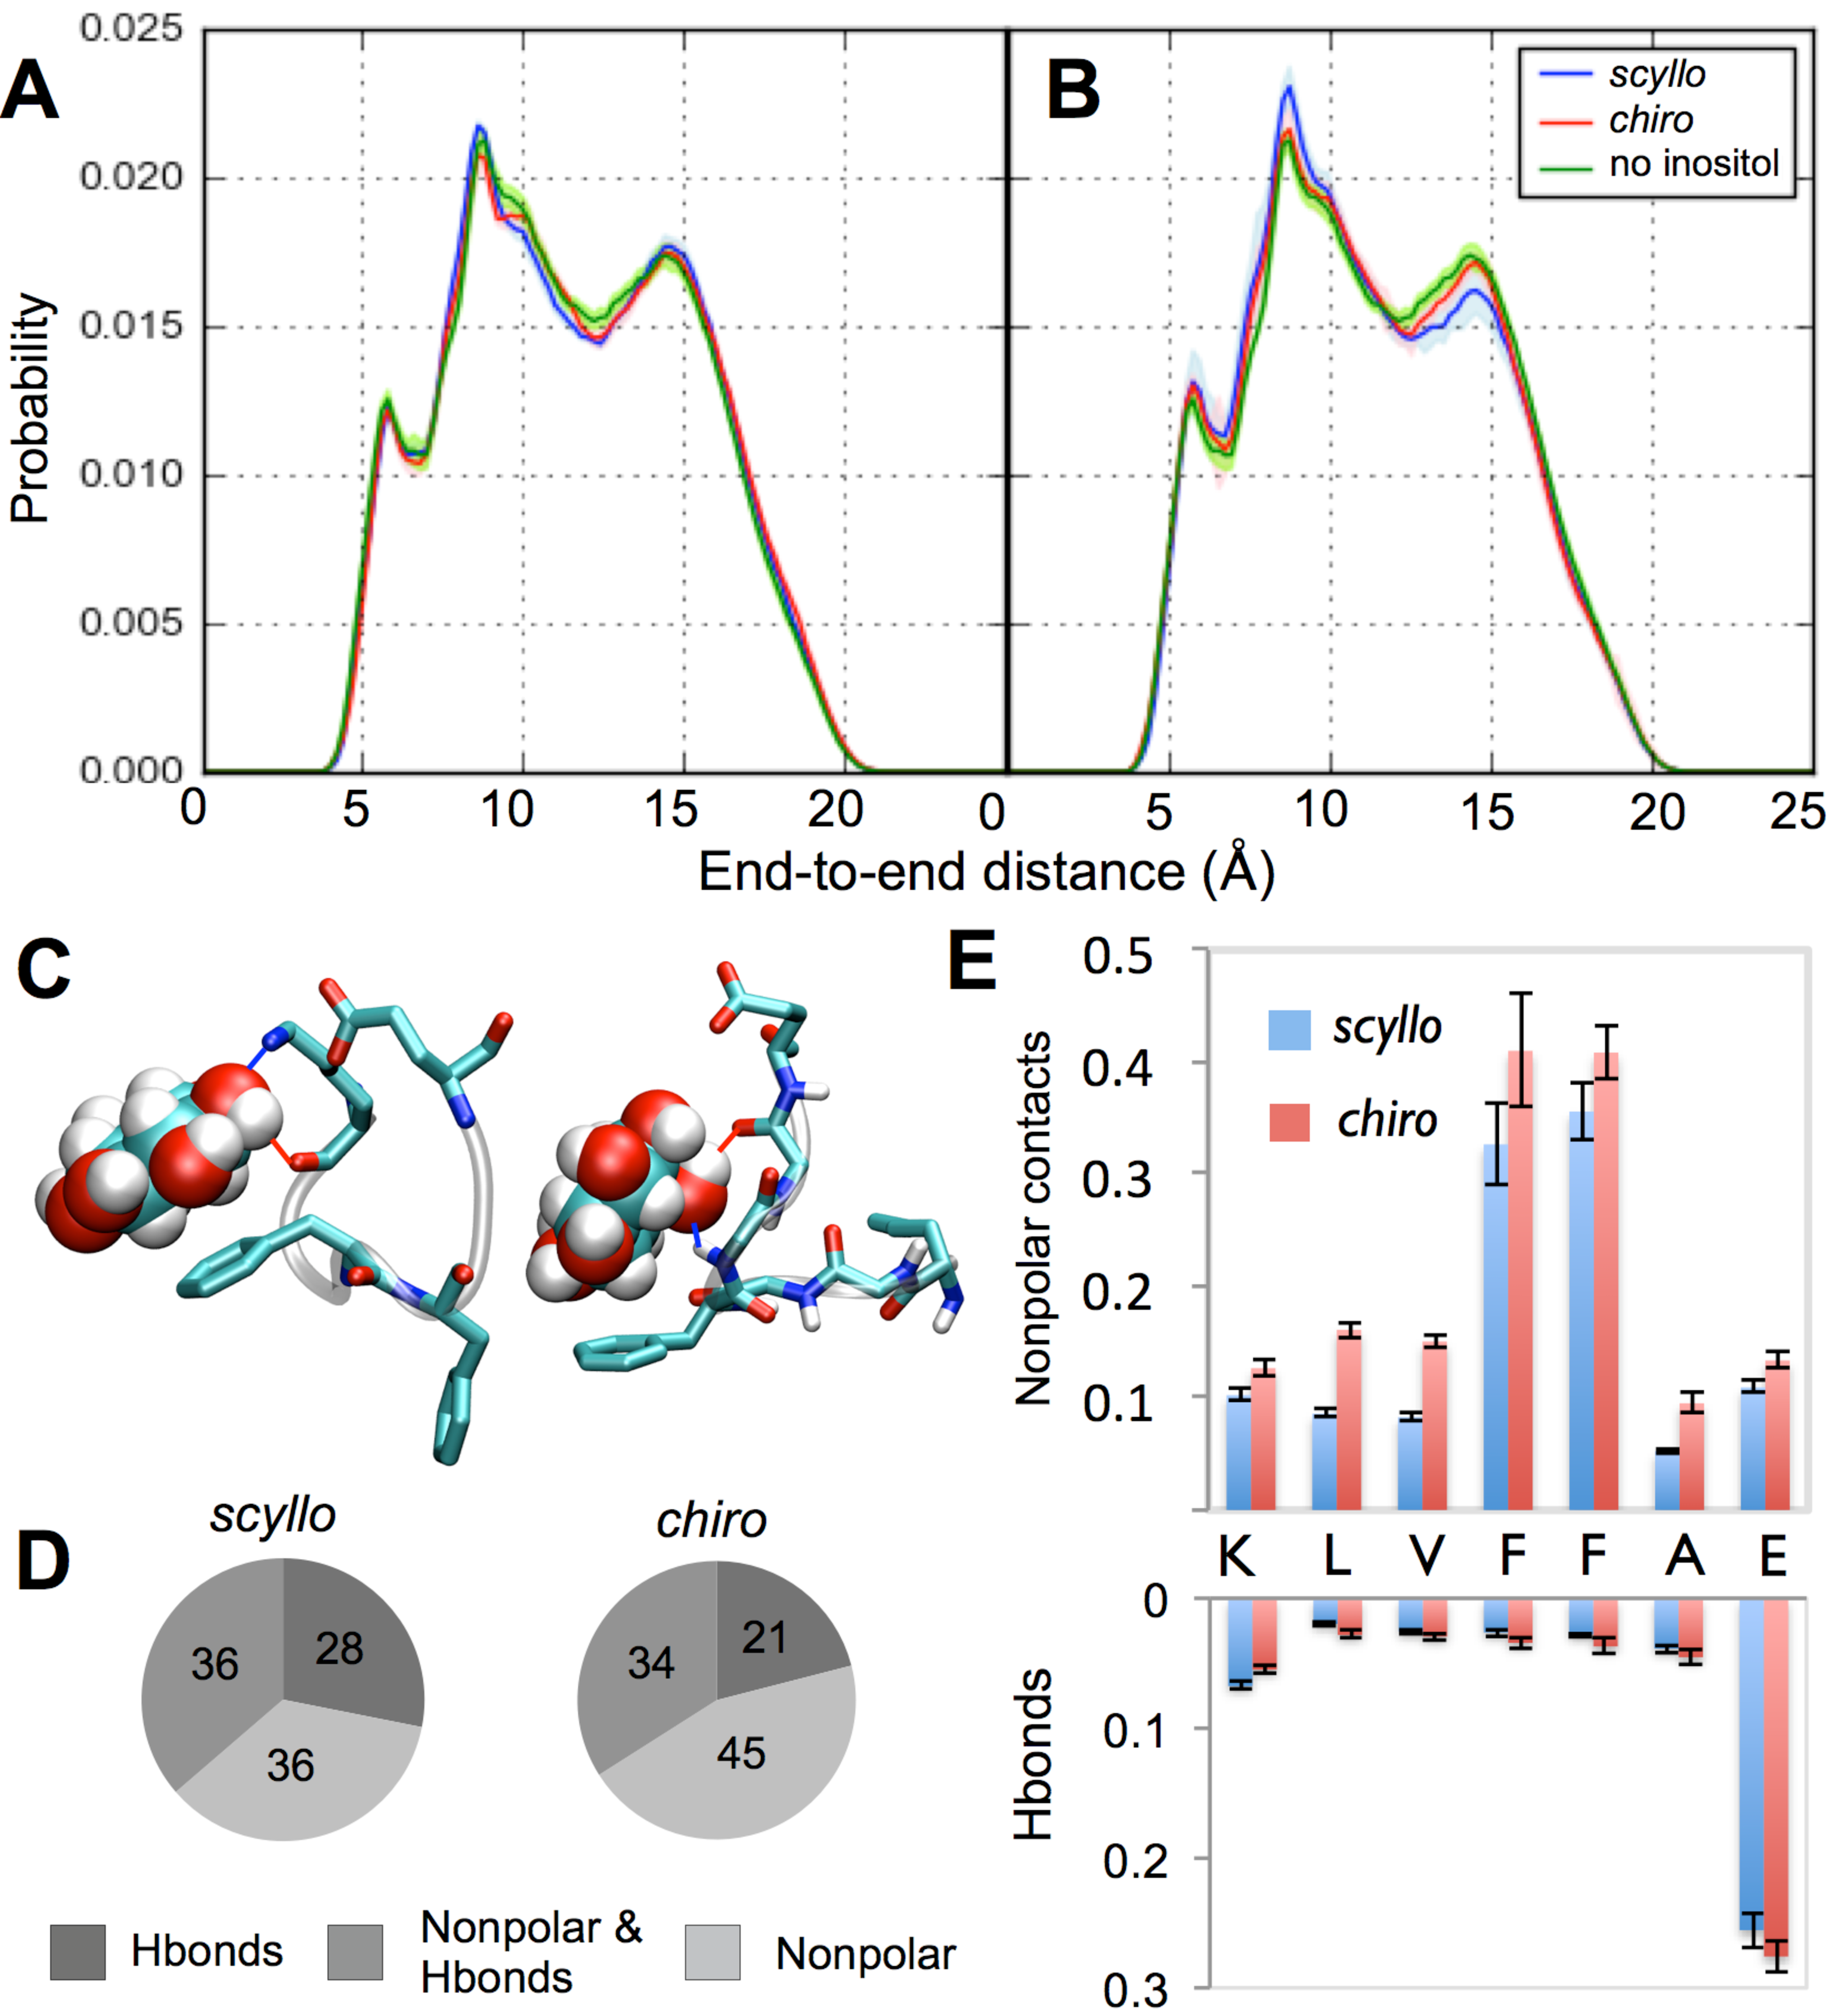
\includegraphics[width=14.6cm]{figures/inos2_figures_monomers_revised.pdf}
\caption{Binding of inositol to an A$\beta$(16-22) monomer.  End-to-end probability distribution of A$\beta$(16-22) successively in pure water and in presence of \emph{scyllo}- and \emph{chiro}-inositol at inositol:peptide molar ratios of (A) 2:1 and (B) 15:1.  (C) Representative snapshots of the different binding modes of \emph{scyllo}- (left) and \emph{chiro}-inositol (right)  to the peptide monomer. Hydrogen bonds between inositol and backbone NH (blue) and CO (red) groups are shown as solid lines. (D) Percent of bound inositol molecules in contact with nonpolar and polar groups at an inositol:peptide molar ratio of 15:1. (E) Time-averaged number of nonpolar contacts (top), and hydrogen bonds (bottom) made by inositol  (at a molar ratio of 15:1) to each residue.}
\label{fig:monomers}
\end{figure}

\begin{figure}
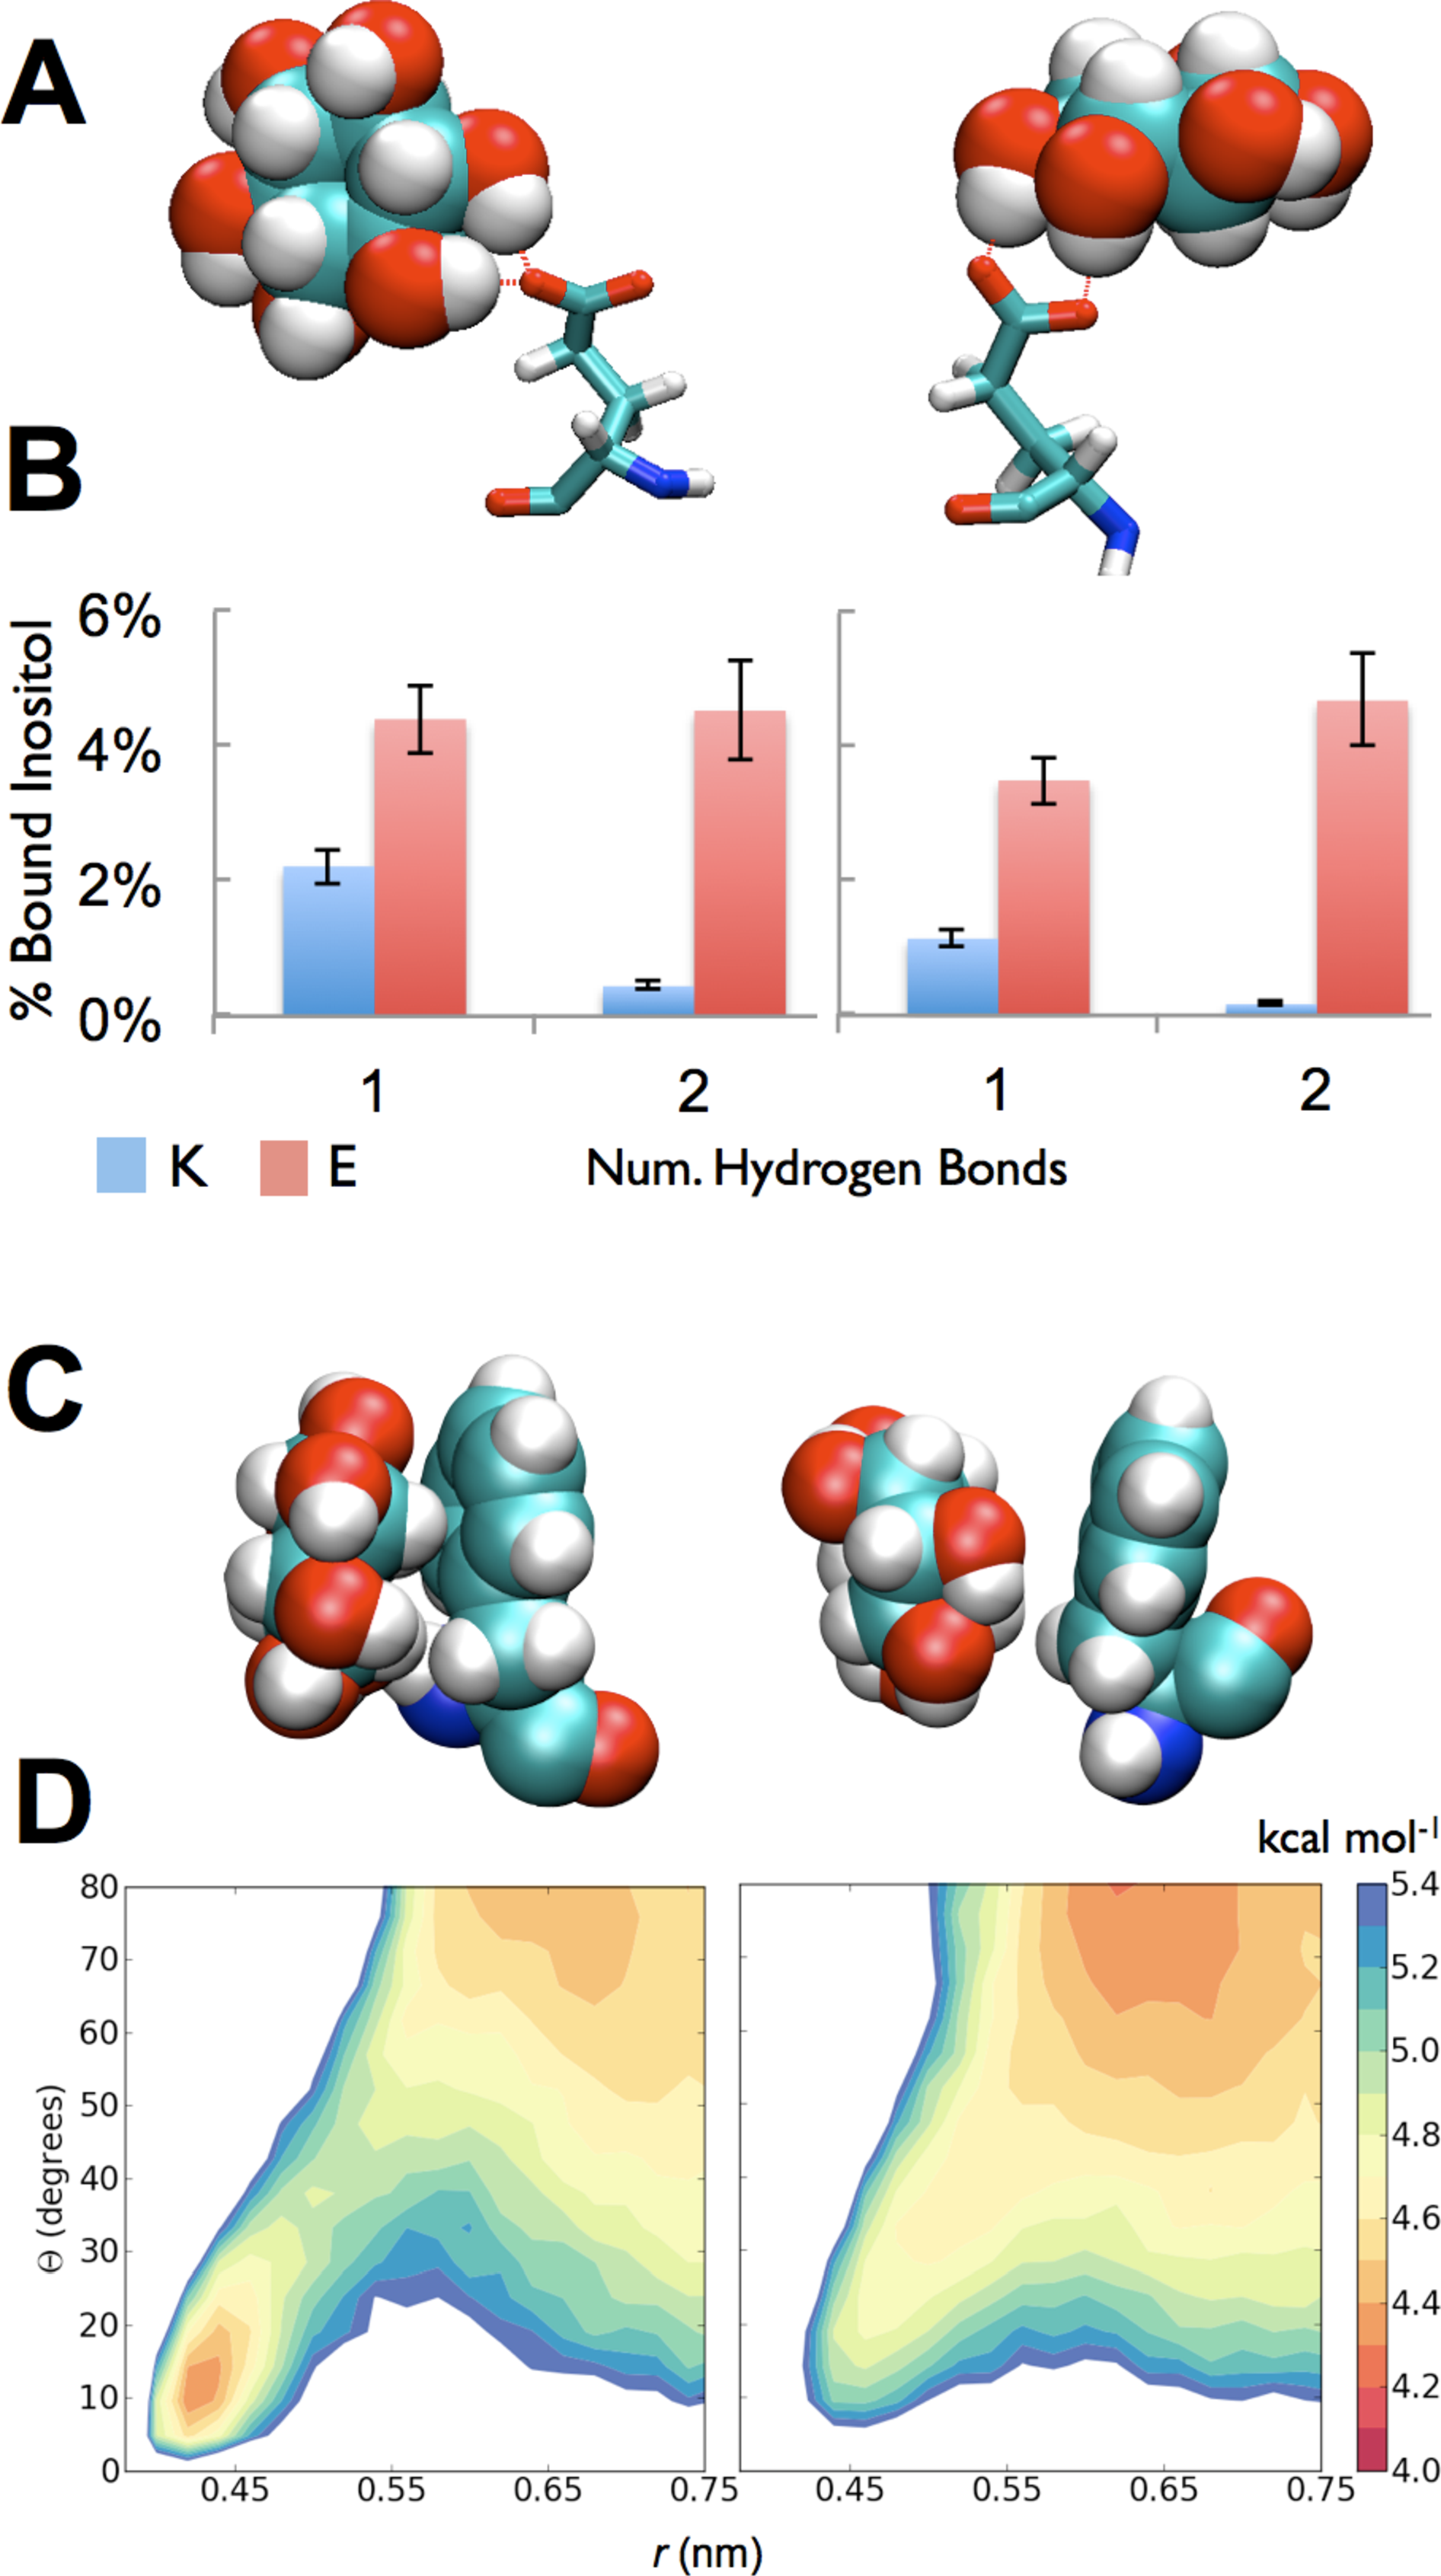
\includegraphics[width=3.185in]{figures/inos2_figures_monomer_residues_pmf_color.pdf}
\caption{Binding of inositol to Glu and Phe dipeptides. Data for \emph{scyllo}- and \emph{chiro}-inositol are shown on the left and right panels, respectively. (A) Examples of snapshots of inositol bound to the carboxylate group of Glu. (B) Comparisons of the probability of inositol hydrogen bonding to the side chains of Lys and Glu. (C) Examples of nonpolar association between Phe and inositol. (D) Potential of mean force (PMF) of inositol with the phenyl ring of Phe relating $r$, the distance between the centers of geometry of the phenyl and inositol rings, to $\theta$, the planar angle between the rings. Contours are drawn at 0.1 kcal$\cdot$mol$^{-1}$ intervals. Face-to-face stacking for \emph{scyllo}-inositol appears on the PMF at $r=0.45$ nm and $\theta=12\degree$.}
\label{fig:monomers_glu_phe}
\end{figure}

\begin{figure}
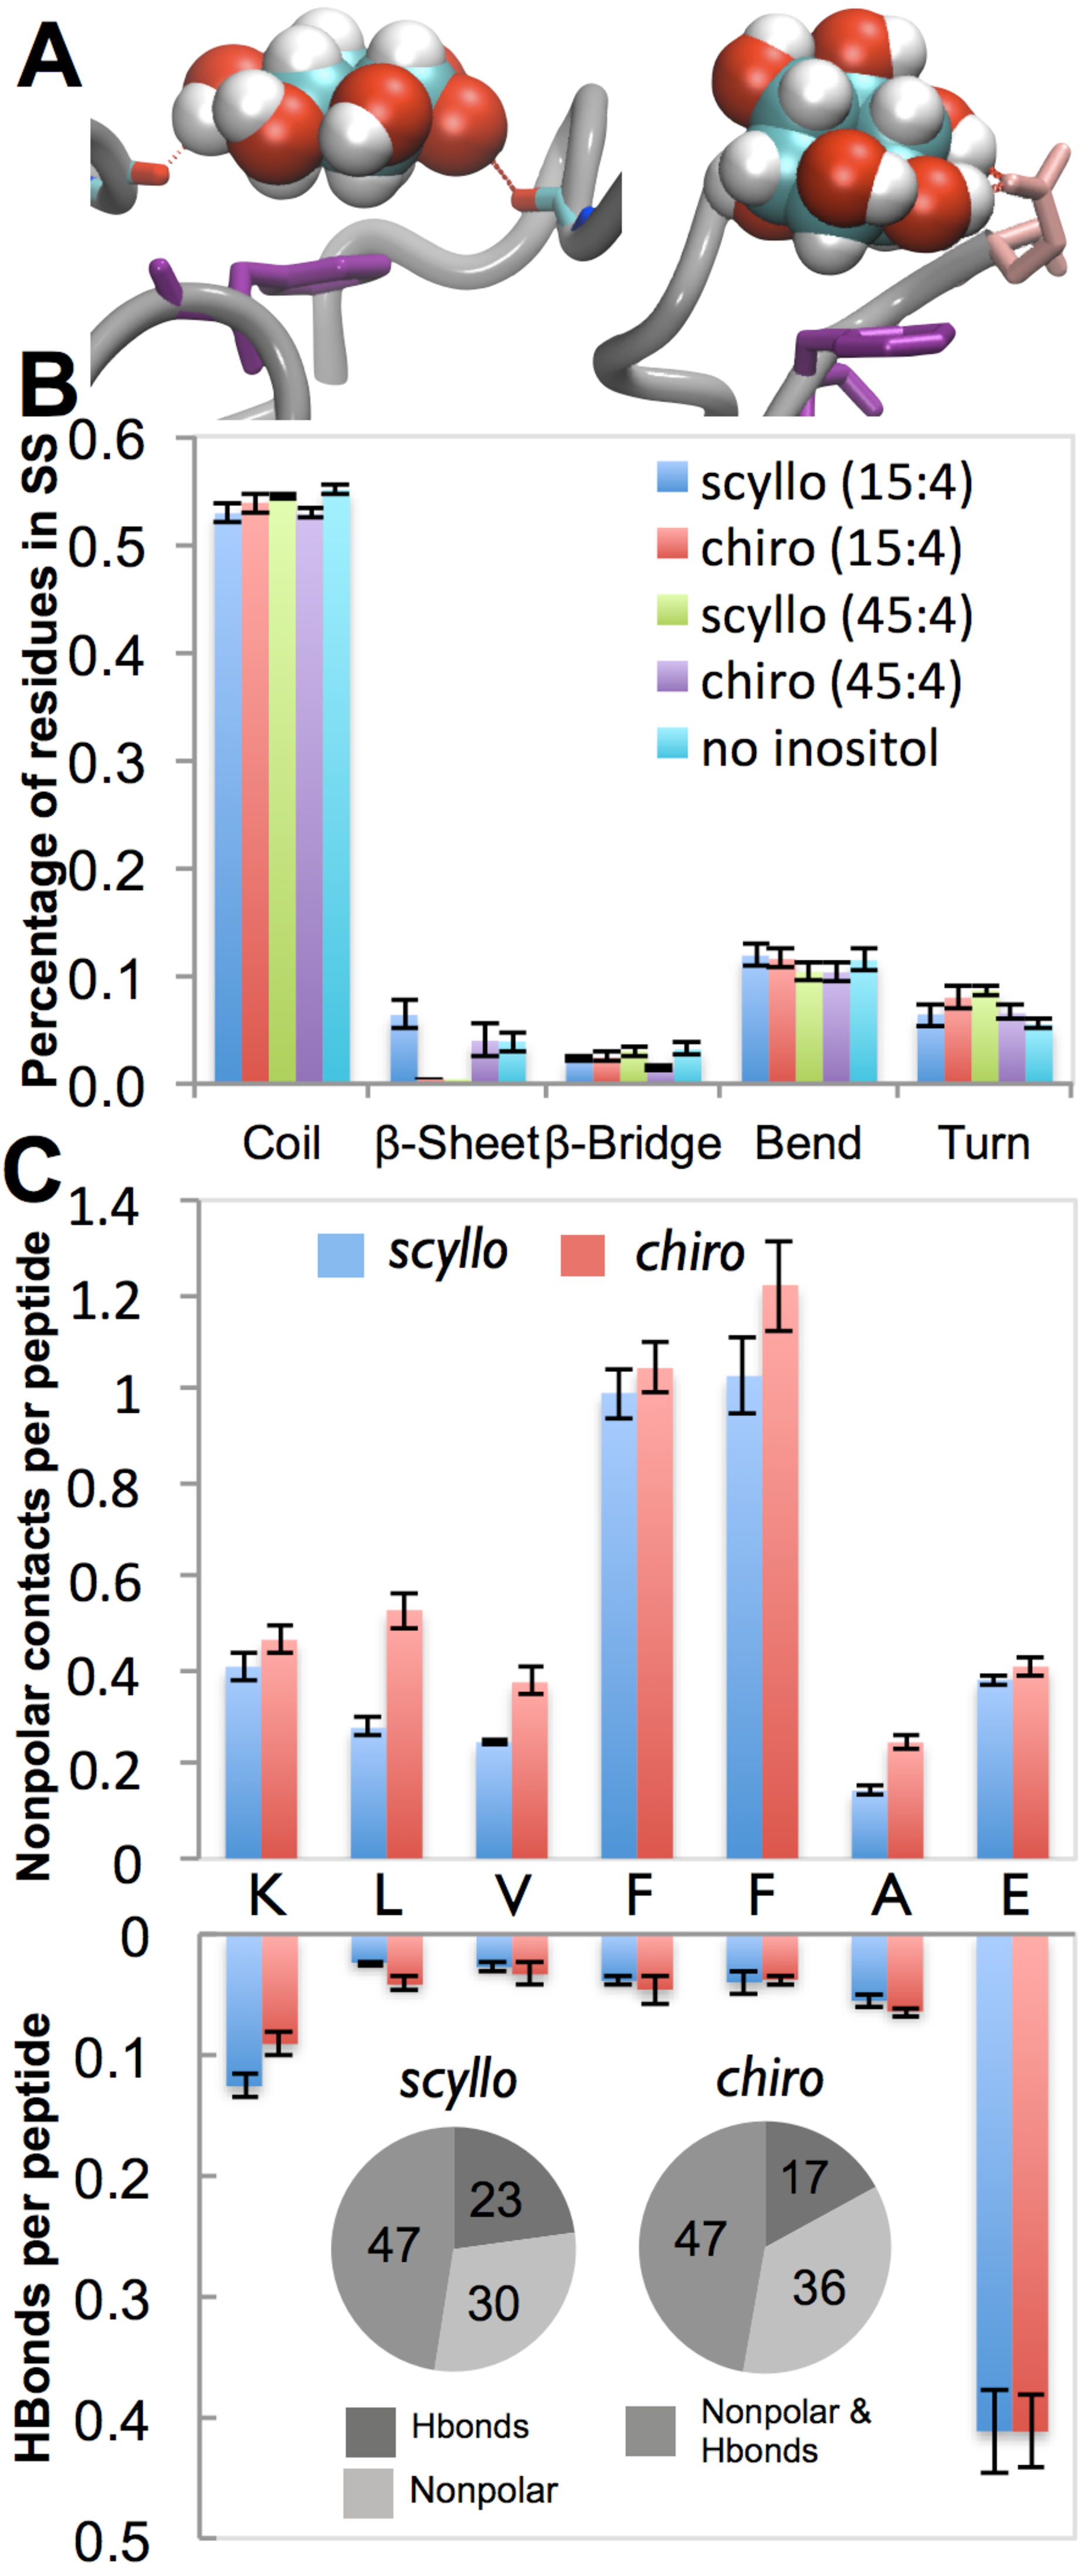
\includegraphics[width=7.96cm]{figures/inos2_figures_disordered_revised.pdf}
\caption{Binding of inositol to a disordered oligomer of A$\beta$(16-22).  (A) Example snapshots of \emph{scyllo}- (left) and \emph{chiro}-inositol (right) involving both nonpolar contacts and hydrogen bonding. (B) Fraction of residues in coil, $\beta$-sheet/bridge, bend, and turn conformations as classified by the DSSP algorithm. (C) Time-averaged number of nonpolar contacts (top) and hydrogen bonds (bottom) made by inositol to each residue (per peptide). Inset: Percent of inositol molecules bound to nonpolar and polar groups of the peptide oligomer at an inositol:peptide molar ratio of 45:4 (inositol concentration of 209 mM).}
\label{fig:disordered}
\end{figure}

\begin{figure}
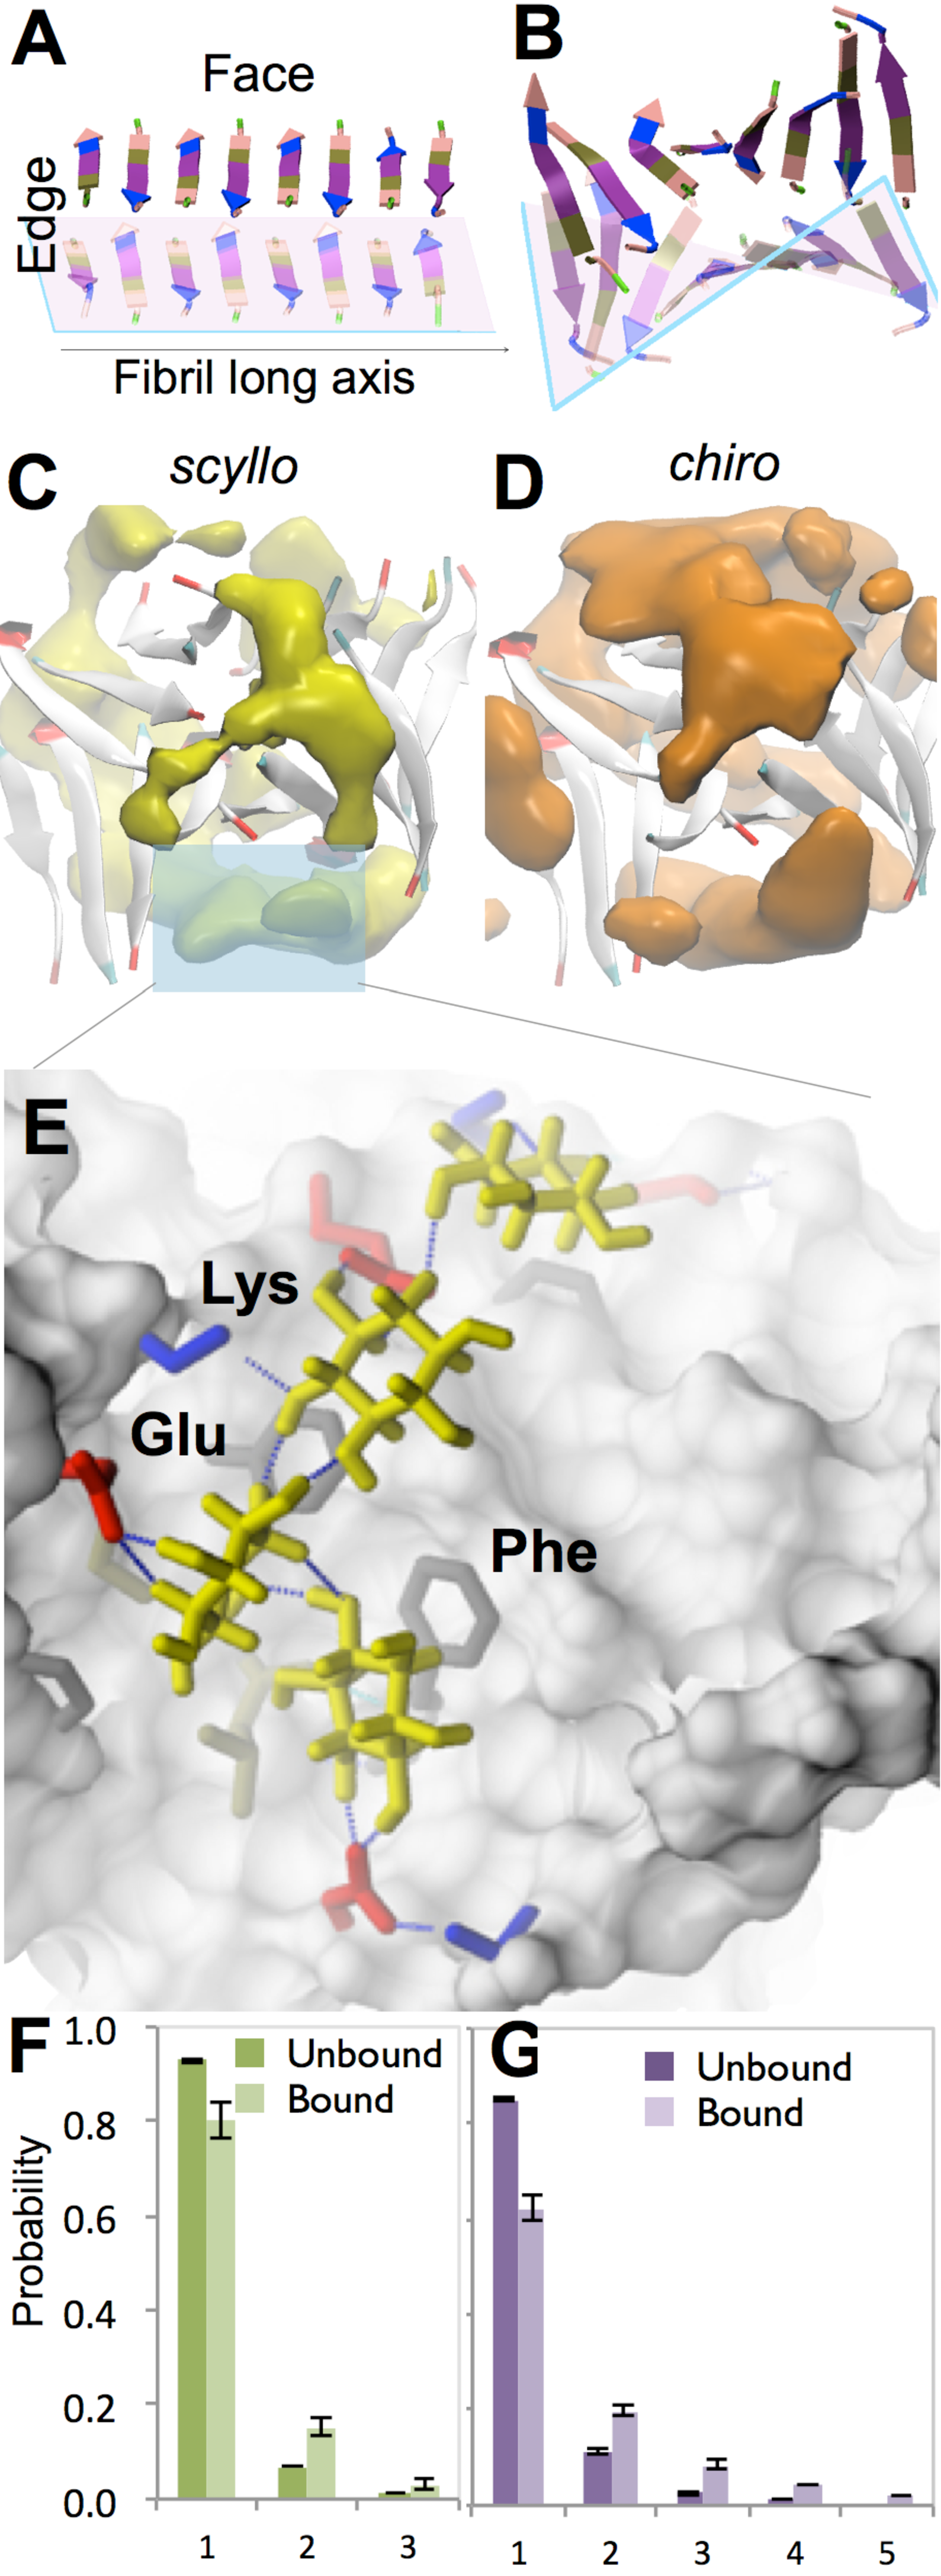
\includegraphics[width=8.1cm]{figures/inos2_figures_beta.pdf}
\end{figure}
\begin{figure}[t!]
\caption{Inositol binding to a $\beta$-oligomer of A$\beta$16-22. Schematic depiction of $\beta$-oligomer twisting: (A) the initial rectangular dual-stacked $\beta$-sheet, evolved into (B) a twisted morphology. Spatial probability density maps of (C) \emph{scyllo}-inositol and (D) \emph{chiro}-inositol are shown in yellow and orange, respectively.  Concentration of inositol is 208 mM and surfaces shown correspond to 7\% inositol occupancy. (E) An example of cooperatively-bound \emph{scyllo}-inositol molecules (yellow) at the surface of the $\beta$-oligomer (grey). Size distribution of bound and unbound clusters of \emph{scyllo}-inositol with the $\beta$-oligomer at inositol concentrations of (F) 62 mM and (G) 208 mM.}
\label{fig:beta}
\end{figure}

\begin{figure}
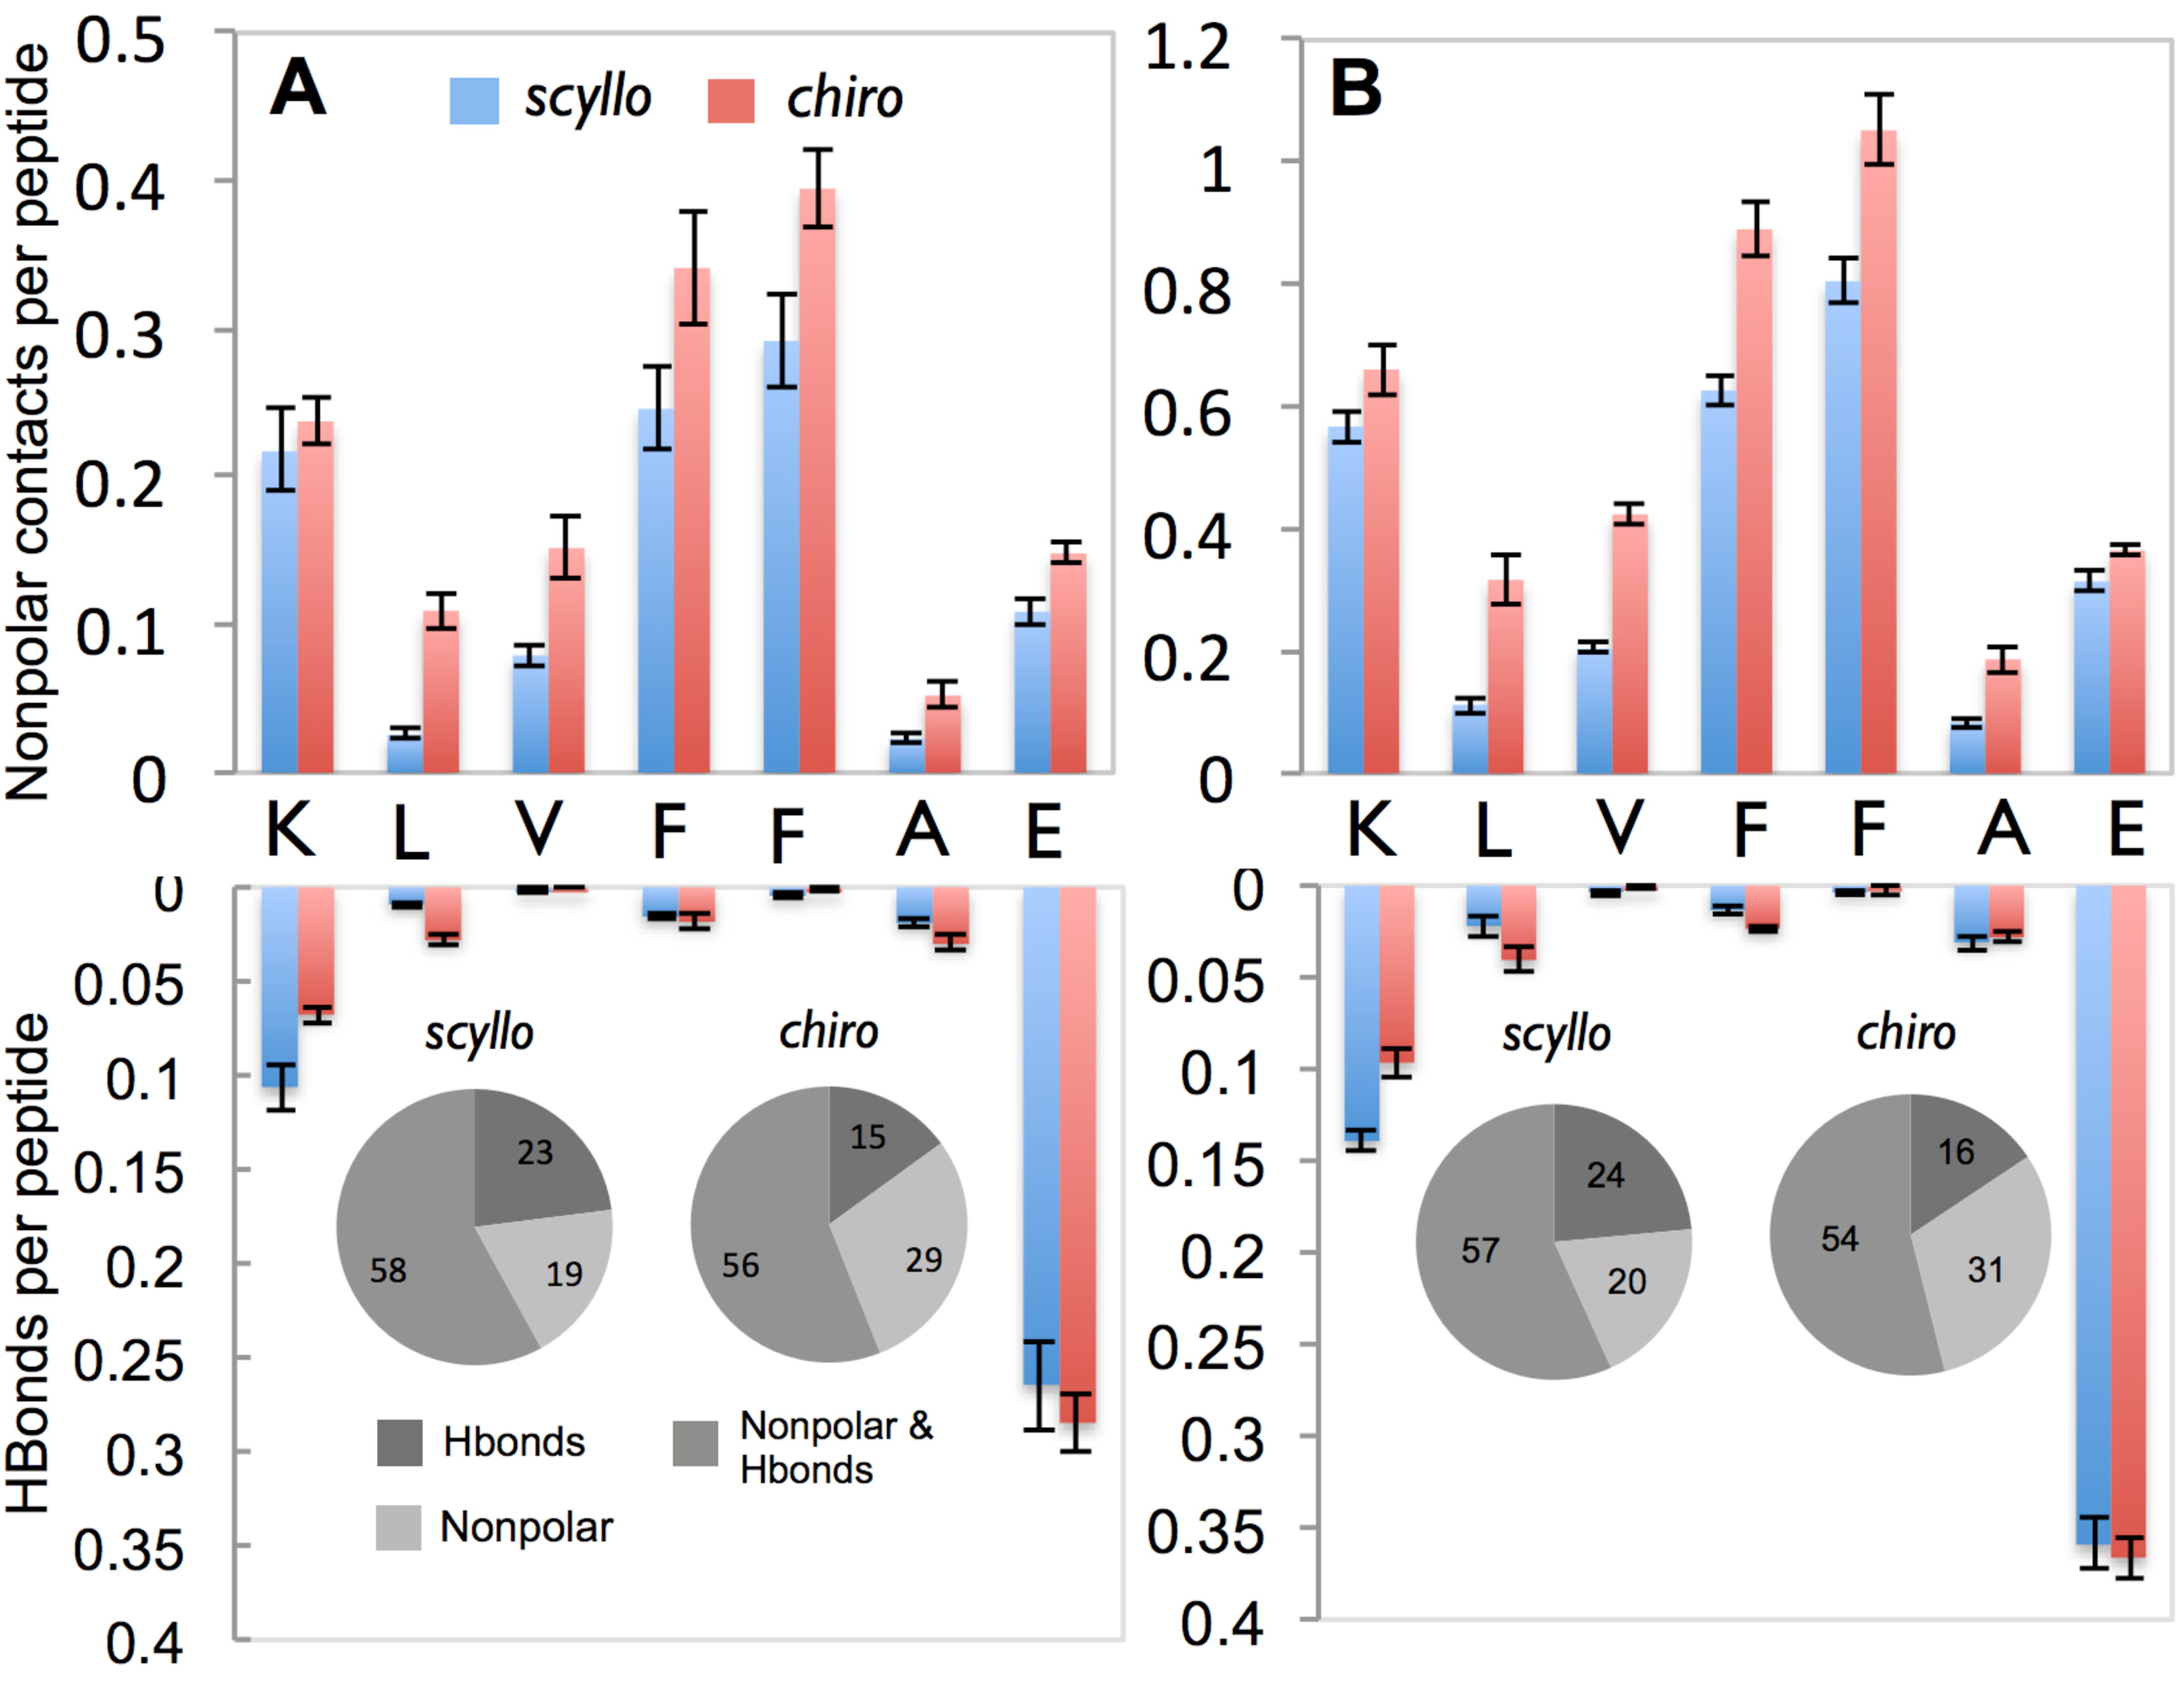
\includegraphics[width=15cm]{figures/inos2_figures_beta_residues_revised.pdf}
\caption{Binding propensity of inositol to nonpolar and polar groups of the $\beta$-oligomer. Average number of nonpolar contacts (top) and hydrogen bonds (bottom), per peptide, made by inositol to each residue of the $\beta$-oligomer. Inset: Percent of \emph{scyllo}- and \emph{chiro}-inositol molecules bound to nonpolar and polar groups of the $\beta$-oligomer.  Inositol is present at a concentration of 62 mM in part A and 208 mM in part B.}
\label{fig:beta_residue_binding}
\end{figure}

\begin{figure}
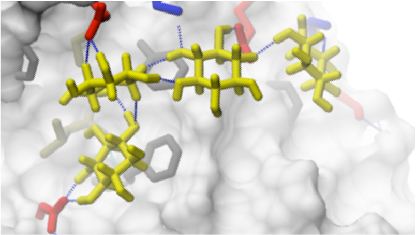
\includegraphics[width=2.78in]{figures/inos2_toc.pdf}
\caption*{Table of Contents image}
\end{figure}

% % Abeta42
% \chapter[A$\beta$42]{Molecular Mechanism of A$\beta$42 fibril inhibition by inositol}

% Some notes
% I found these pretty neat ref articles on sciencedirect
% http://www.sciencedirect.com.myaccess.library.utoronto.ca/science/article/pii/B9780444519672001550
% http://www.sciencedirect.com.myaccess.library.utoronto.ca/science/article/pii/B9780444519672000581
% http://www.sciencedirect.com.myaccess.library.utoronto.ca/science/article/pii/B9780444519672000313
% http://www.sciencedirect.com.myaccess.library.utoronto.ca/science/article/pii/B0080437486011592

	
\section{Summary}
Alzheimer's disease (AD) is a severe neurodegenerative disease with no cure. Currently, one method of targeting the underlying disease is to prevent or reverse the amyloid formation of A$\beta$42, a key pathological hallmark of AD. A small-molecule novel drug candidate, Scyllo-inositol, is a polyol small-molecule that exhibits stereochemistry dependent inhibition of the formation of fibrils in vitro.  Furthermore, recently completed phase II clinical trials demonstrated that scyllo-inositol achieved target drug levels in the cerebral spinal fluid (CSF) of AD patients, a main challenge for AD drug candidates to overcome.

Despite its promise as a therapeutic for AD, the mechanism of action of scyllo-inositol at the molecular level is currently not understood.  We perform extensive atomistic molecular dynamics simulations of scyllo-inositol and its inactive stereoisomer, chiro-inositol, glucose, and the osmolyte protein stabilizer, glycerol, with the full length A$\beta$42 protofibril.  From our simulations, we characterize the stereochemistry-dependent binding modes of these three cosolutes on the structure and aggregation of A$\beta$42 protofibrils.  Our results provide molecular insight for the rational design of small-molecule inhibitors of A$\beta$42 and other amyloid-based diseases.

  \textbf{Keywords}:
	amyloid computational
	amyloid inhibition
	small molecule amyloid inhibition
	amyloid disaggregation
	inositol
	surface binding
	weak interactions
	carbohydrate like interactions

\section{Introduction}

% Why Abeta42 
\abeta42 is the pathological hallmark of Alzheimer's Disease (AD) and forms the largest proteinaeous component of plaques in the brain of AD patients. \abeta\ peptides are produced from the cleavage of amyloid precursor protein (APP) in isoforms with lengths of 33 to 42 residues. Although \abeta42\ and \abeta40\  peptides differ in length only by two residues, they have a number of notable differences: \abeta42\ is found to display significantly higher aggregation propensity\cite{Jarrett:1993vm,Fukumoto:1996vi,Finder:2010jw} and cellular toxicity than \abeta40\ peptides.\cite{ElAgnaf:2000hp,Mucke:2000uqa}  Furthermore, they are found to form fibrils via distinct pathways.\cite{Bitan:2003ut,Sanchez:2011bj,Bitan:2003p1781}
% This difference in the two residues confer significant differences in their aggregation propensity and toxicity.
% Do I really need to talk about polymorphism?
% Although the \crossbs\ is the core tertiary structure found for all amyloid fibrils, fibrils exhibit polymorphism at the residue-level depending on their formation conditions.\cite{Wu:2010p3553} \textbf{where they different polymorphs?} Different amyloid fibril structures may exhibit different toxicities.\cite{Paravastu:2009fi,Wu:2010p3553}
% Fibril structures of \abeta40\ and \abeta42\ were also found to be similar.\cite{Wu:2010p3553} There are brain derived structures of \abeta40, their structures are different from the synthetic ones because of polymorphism. 


% Rationale for studying the Abeta42 protofibril system	-- there is all this abeta40 stuff simply because its easier to work with these peptides, but then abeta42 is the actual important peptide that people should be looking at!
In the past few years, many studies have probed the aggregation properties of \abeta40. Fibril models of the \abeta40\ peptide derived from solid-state NMR (SSNMR) indicate that protofilaments of \abeta40\ contain 2 to 3 layers.\cite{Wu:2010p3553,Tycko:2010iz} By contrast, much less is known about the fibril structure of \abeta42. A SSNMR model of the fibril of \abeta42\ was recently proposed by Luhrs et al. In that model, N-terminus of \abeta42\ in the fibril was found to be unstructured.\cite{Ahmed:2010p5694} A previous MD simulation study of \abeta42\ protofibrils in pure water suggests that residues 17 to 42 are predominantly involved in the stability of the core structure of the fibril.\cite{Masman:2009p6410}

% \textbf{Small molecules are promising candidates for the treatment of AD. Many of them have been found to display anti-aggregation activity, including osmolytes.} 
In recent years, drug development and research efforts have been directed towards the development of therapeutic agents to prevent the self-aggregation and amyloid formation of A$\beta$, a promising treatment approach to target the underlying disease.\cite{Masters:2006p183,Citron:2010p214,Dasilva:2010p25} As a result, many different types of \emph{in vitro} amyloid inhibitors have been discovered, including peptides,\cite{EsterasChopo:2008p219,Sciarretta:2006p181,Chalifour:2003p161,Scrocchi:2002p178,Soto:2007dm} immunotherapies,\cite{Janus:2000p198,Solomon:2010p177} polyphenolic molecules,\cite{Masuda:2009p205,Berhanu:2010p230,Ehrnhoefer:2008p8} and other small molecules.\cite{Hawkes:2009p189,Masuda:2009p205,Necula:2007p227,Nitz:2008p13} These approaches have been reviewed in detail elsewhere.\cite{Citron:2010p214,Dasilva:2010p25}

\emph{scyllo}-Inositol is a small-molecule inhibitor of A$\beta$42-fibrillation developed for the treatment of AD.\cite{McLaurin:2006p29,McLaurin:2000p64,Fenili:2007p182,Ma:2012jk} 
Inositol is a class of cyclohexylpolyols, of which eight out of nine stereoisomers are commonly found in nature. \emph{scyllo}-Inositol, with all hydroxyl groups equatorial,  is the only isomer with two planar hydrophobic faces. By contrast, its diastereisomer, \emph{chiro}-inositol, with two adjacent axial hydroxyl groups, has two nonplanar  hydrophobic faces.  Importantly, \emph{scyllo}-inositol was demonstrated to prevent and reverse AD-like symptoms in a transgenic mouse model of AD.\cite{McLaurin:2006p29} Because of the positive CNS bioavailability and favorable \emph{in vivo} toxicity profile of inositol, both of which are rare and essential properties of putative AD drug candidates, inositol-based therapies represent unique and promising approach for the treatment of AD. Phase II of clinical trials for \emph{scyllo}-inositol (ELN0005) in North America was fast-tracked in 2007 by the United States Food and Drug Administration and was completed in 2011.\cite{Salloway:2011im,Ma:2012jk}

\emph{In vitro}, inositol displays stereochemistry-dependent inhibition of A$\beta$42 fibrils: \emph{scyllo}-inositol was shown to inhibit A$\beta$42 fibrillation at concentrations of 1 - 5 mM,\cite{McLaurin:2000p64} whereas \emph{chiro}-inositol is inactive below molar concentrations.\cite{Janus:2000p198} Moreover, upon incubation of monomeric A$\beta$42 with \emph{scyllo}-inositol, circular dichroism spectroscopy indicated the formation of $\beta$-sheet structure at an inositol:peptide molar ratio of 25:1.\cite{McLaurin:1998p176} 

Although inositol stereoisomers have been proposed to inhibit amyloid formation by directly interacting with either monomers or non-fibrillar aggregates to ``cap off'' fibril growth,\cite{Janus:2000p198} the molecular basis of the effect of \emph{scyllo}-inositol and its stereoisomers on A$\beta$42 amyloid formation is currently unknown.
% \cite{Nikolic:2011p185,Rauscher:2006p43,Li:2012p853,Rauscher:2010p5682,Sgourakis:2011hy,Wang:2005do,Cino:2011ff}

Molecular dynamics (MD) simulations are well-suited for studies of disordered proteins and can provide atomic-level insight into the mechanism of inhibition of peptide self-aggregation by small molecules. MD simulations were previously employed to examine the binding mechanism of other small-molecule inhibitors such as polyphenols,\cite{Lemkul:2010p23,Wang:2010p204} non-steroidal anti-inflammatory drugs\cite{Raman:2009p47,Takeda:2010p34}, and the well-known amyloid dye thioflavin T\cite{Wu:2008ds,Wu:2011fd} to monomers and/or fibrillar forms of A$\beta$\cite{Liu:2009p213}. 

Because of the existence of multiple aggregation states, small-molecule inhibitors may have multiple modes of action and may act by binding either to monomers\cite{Ehrnhoefer:2008fd} or to non-fibrillar or fibrillar oligomers\cite{Buell:2010p9457} in the fibrillation pathway. Furthermore, their inhibitory activity may also be affected both by the concentration of the ligand and by the ligand:peptide molar ratio.\cite{Wang:2010p204,LeVine:2005cv}  

% However, thus far, few MD simulation studies have examined the effect of ligand concentration on different relevant aggregation states along the amyloid fibrillation pathway.\cite{Wang:2010p204}

% \textbf{Do I need this? Say why its important to look at binding for Abeta42 instead}
% On the basis of current high-resolution structural data, there are several differences between the fibril structures of A$\beta$42 and A$\beta$40.\cite{Ahmed:2010p5694} \textbf{ADD: what are their differences}

% In recent years, scyllo-inositol, a small-molecule polyol, has demonstrated promise as a potential therapeutic of Alzheimer's Disease. scyllo-inositol displays stereochemistry-dependent activity of amyloid inhibition of \abeta42.REF In studies with a mouse model of AD, scyllo-inositol was shown to prevent and reverse the on-set of AD.REF 

% Where would this idea fit? Small-molecule modulators of amyloid formation may be classified into those that accelerate and / or stabilize amyloid formation and those that displace the equilibrium towards the disaggregated state (inhibitors of amyloid formation).

In two previous studies, using MD simulations, we successively examined the binding mechanism of scyllo- and chiro-inositol with peptide and aggregate states of model amyloid-forming peptides and A$\beta$(16-22), the central hydrophobic core of A$\beta$. Weak and stereochemistry independent binding of inositol with the peptidic backbone was found, with binding constants in the range of 0.1 - 1 M, indicating that inositol is unlikely to inhibit amyloid formation by binding the peptidic backbone alone.\cite{inos1} However, in our study involving A$\beta$(16-22), inositol was found to preferentially bind to the surface of $\beta$-sheet oligomers, but only weakly to those of disordered or monomeric forms. Furthermore, inositol was found to adopt cooperative, high avidity binding modes with $\beta$-oligomers with binding constants commensurate with the \emph{in vitro} inhibitory concentrations.  Taken together, the results from our previous studies indicate that inositol is likely to disrupt amyloid fibrillation by binding to  $\beta$-sheet oligomers of A$\beta$.

\textbf{Need a lot more detail here} In this study, we examine the binding mechanism of inositol stereoisomers, scyllo- and chiro-inositol, along with glucose and glycerol, with the SSNMR model protofibril of the full-length \abeta42.  Both glucose and glycerol affect fibrillation of A$\beta$42\ at concentrations of more than 1 M. 

\textbf{I think it makes more sense to talk about osmolytes here} Organic osmolytes such as glycerol and glucose, are small molecules that stabilize the folded state of proteins. Examples include TMAO, glycerol, and are thought to do so via the preferential exclusion mechanism.\cite{Bolen:2001im}  In recent years, osmolytes that stabilize the folded state of proteins, have been found to modulate amyloid formation\cite{Sukenik:2012dv,Sukenik:2011p8778}. TMAO,\cite{Seeliger:2013cj}betaine,\cite{Natalello:2009fn} glucose,\cite{Fung:2005p2008} trehalose\cite{Nayak:2009fr} and glycerol\cite{Sukenik:2011p8778} been found to modulate amyloid formation and peptide aggregation.\cite{Liu:2005km,Sukenik:2011p8778,Fung:2005p2008} \textbf{But so what? There is no logical link presented for this piece of information right now}
% In particular, glycerol is able to slow the kinetics of fibrillation (I don't think this is correct -- check this again).\cite{Yang:1999ws}This paper did a study on myo-inositol, but from a fast scan I wasn't able to figure out what their conclusions for myo- and other polyols are.\cite{Macchi:2012ci}

In this paper, we present results which provide insight into the structure-activity relationship of inositol in the inhibition of A$\beta$ amyloid formation, and will ultimately lead to forming a pharmcophore for treating AD and related neurodegenerative disorders.

\textbf{The rationale of my study:} Thus far, cosolute binding to amyloid fibrils have not been examined. It is known that several cosolutes do not inhibit amyloid formation.  It is informative to compare their binding with known inhibitors of amyloid formation in that differences in their binding could further explain the mechanism of inhibition.

Because our previous studies suggest that inositol is unlikely to interact with the monomer and disordered oligomers, and that the likely interaction partner of inositol are beta-sheet-aggregates of Abeta42, in this study we examine the binding of inositol, and cosolutes glycerol and glucose with the protofibrillar oligomer of full-length Abeta42.

% For now, I removed the table of simulations.  There is no variation in the system run times or molar ratio. Can just mention this or put this table in supplementary information.
  
\section{Material and Methods} % (fold)
\label{sec:material_and_methods}

The pentameric solid-state NMR model of A$\beta$(17-42) from Luhrs et al. (PDB code: 2BEG) was used as the starting structure in our simulations.\cite{Luhrs:2005p4900} In the PDB structure, residues 1 to 16 were truncated in the model because they are disordered.\cite{Luhrs:2005p4900} Because the truncation at the N-terminal ends of the peptides is artificial,  acetyl groups to the peptides, yielding an uncharged N-terminal end of the fibril. The acetyl groups were modeled onto the fibril using PyMol. Titratable amino acids were assigned charged states at the physiological pH. 10 sodium ions were added neutralize the remaining charges in the system. To mimic experimental conditions, 0.15 M of salt were added. Protein and solvent were represented by the OPLS-AA/L force field\cite{Jorgensen:1996vx} and the TIP3P water model,\cite{Jorgensen:1983p8768} respectively.  The  extended OPLS-AA force field for carbohydrates was used to model inositol stereoisomers and glucose.\cite{Damm:1997tla}

All MD simulations were performed in the NpT ensemble using the GROMACS simulation package version 4.0.x.\cite{Hess:2008p5353} The leapfrog Verlet integration algorithm was used with an integration timestep of 2 femtoseconds. Long-range electrostatic interactions were calculated using Particle Mesh Ewald (PME) summation with a Fourier grid spacing of 0.15 nm and a real-space cutoff of 1.3 nm.\cite{Darden:1993p8963} The short-range nonbonded van der Waals interactions were switched to zero from 1.1 nm to 1.2 nm. The temperature was controlled at 300 K using the Nose-Hoover thermostat. Pressure was controlled by the Parrinello-Rahman barostat at 1 atm with a coupling constant of 4.0 ps. The SHAKE algorithm was used to constrain covalent bonds containing hydrogens.\cite{Ryckaert:1977p9357}

In all simulations, a cubic box was used and periodic boundary conditions. Prior to data collection, 500 steps of energy minimization using the conjugate gradient algorithm was first performed, followed by a 200 ps long equilibration in the NVT ensemble and a 2 ns long equilibration with isotropic pressure coupling (NPT ensemble). The center of mass (COM) rotation and translation were removed at every step.

A set of ten 0.250 $\mu$s simulations of the protofibril of \abeta42 were performed,  successively, in pure water and in the presence of scyllo-inositol, chiro-inositol, glycerol and glucose. The ligands were present at either a ligand:peptide molar ratio of  15:5 or 64:5, yielding a total sampling time of 12.5 $\mu$s.

\subsection{Analysis Protocol}
GROMACS analysis tools g\_rmsd and g\_rmsf were used to calculate the root mean square deviation in the fibril backbone and root mean squared fluctuation, respectively.  Spatial probability density of bound inositol were calculated using the volmap tool in Visual Molecular Dynamics software package (VMD). 

Nonpolar contacts between inositol and fibril were defined by a carbon to carbon cutoff of 0.X nm. The DSSP hydrogen bonding criteria were used to determine the existence of a hydrogen bond.  Secondary structure analysis was performed using do\_dssp using the DSSP algorithm.

Interchain hydrogen bonds (s1 - s2, s2 - s3, s3 - s4, s4 - s5) were computed between adjacent strands in the fibril using g\_hbond.  Hydrogen bonding criteria used acceptor-donor heavy atoms with distance less than 0.35 nm and hydrogen-donor-acceptor angle of less than 30 degrees (CHECK THIS).
	
% Contact map of inositol to A$\beta$42
Binding constants are calculated by assuming the reaction,

% Equations used in the KLVFFAE paper
\[ \left[ Protein\cdot Inositol \right] \rightleftharpoons \left[ Protein \right] +\left[ Inositol \right] \]

Where,

\[ K_{d} = f_{ub}\frac{\left[ Protein \right]\left[ Inositol \right]}{\left[Protein \cdot Inositol\right]} \]

% Equation converting population to free energy
% $\mathit{W}=-RT\ln\rho\left(r,\theta\right)$
% $\rho\left(r,\theta\right)$

\section{Results}

\subsection{Protofibrillar morphology}
%Here I can show the RMSF and RMSD and the secondary structure information.  The point is to show that the protofibril stays in tact or not.  If intact, then say that it did not break up the protofibril on the timescale of our simulations.
%
%The technical details involve getting all this data into a columnar form.  First plot the curves separately to identity outliers if any and see why they've deviated by looking at the trajectories for making further hypothesis.

\subsubsection{Protofibrillar morphology}
We first examine the global structural properties of the fibril fragment by looking at the fibril RMSD and RMSF. The NMR model starting structure was used as a reference.  In the absence of inositol, the RMSD from the fibril NMR model for most, but not all of the replicas plateau to a value of about 0.5 nm beginning at about 120 ns (Figure RSMD). The fibril remained aggregated in the simulations.  Note that there could be rare events (but I haven't looked into this too much) - Note that I need to discuss the unravelling in more detail.

Figure RSMD: RMSD of the fibril backbone showing the stability of the SSNMR A$\beta$ fibril in solution.

RSMF (root mean squared fluctuations) of the residues along each chain in the protofibrils show that the protofibrillar aggregate is dynamic in the simulation [Still vague be more specific, why is this significant?]. However, the $\beta$-sheet core of the protofibril stays in tact throughout the simulation. (Figure: RMSF)

\textbf{Figure RSMF}: RMSF of the fibril backbone showing the stability of the SSNMR A$\beta$ fibril in solution.

The dynamics of the protofibril in the presence of cosolutes (ligands)
RMSD vs time of the protofibril measured with rest to the initial starting structure shows that over the course of 250 ns the protofibril stabilizes at 5 Angstroms, indicating that the "arrangement" of the protofibril are all similar in the presence and absence of ligands.  The similarity in the average RMSD of the fibril measured in the presence and absence of ligands, suggesting that the solutes do not significantly perturb the structure of the protofibril. RMSF versus time shows the deviation of each residue away from its average position in the protofibril these fluctuations are all quite similar in the presence of cosolutes. Taken together, our results suggest that fibril morphology is not perturbed in the presence of inositol and cosolutes.


% Hypothesis: The chains at the ends of the fibril are more ‘mobile’ than the chains in the middle. Are the middle strands more likely to be fully hydrogen bonded? Are the side strands more likely to have their backbone hydrogen bonds broken?  Do any of the strands come off / lose all backbone hydrogen bonds ?
	
In some of our replicas, the edge strands are more mobile than the inner strands, and can unwind and partially detach from the rest of the protofibril over the course of the simulation.  The strands at the end of the fibrils show a significant decrease in their interchain hydrogen bonding. (Note need to be careful here because the end chains have less HBs because they don't have flanking peptides) (Figure: interchain hbonding). 

Stability of the fibril in the presence of ligand. Does glycerol stabilize the aggregate? Does glucose stabilize the fibril? Ab42 is stable at both ligand:peptide ratios of 3:1 and 13:1, suggesting that fibrillar aggregate is not disaggregated by ligands over the time scale of the simulation. Note that these observations of the fibril dynamics such as chain unwinding are not correlated with disruption caused by ligand binding as they occur in the control simulations as well.

\textbf{Secondary structure analysis by DSSP}. Inositol does not appear to affect the secondary structure of the residues in the protofibril.  By eye, looks like there is no major differences in water, glycerol, glucose and inositol (NEED more quantitative description)
Figure: Number of residues in secondary structure versus time.  Y-axis is number of residues in a particular SS conformation. 	

% More advanced structural analysis?
% Any large scale motions?
% Worthwhile doing PCA?
% Most likely not meaningful? (probably too noisy)

%Which residues most frequently bound \\
%
%Over all binding modes.  Use the spatial probability maps to demonstrate this \\
%Are there binding hot spots? If so where and what are they? [in the discussion relate these findings to the mechanism of amyloid formation]
%
%Mostly nonpolar or polar? \\
%
%Do the molecules Cluster? If so, do cluster sizes differ? For example do glycerol and glucose  cluster a lot less? If there are differences in this mechanism could have implications in the mechanism of amyloid formation. \\
%
%How do the results compare with my previous results [discussion?] \\
%
%Does any of these molecules target the fibril core? [discussion?] \\
%Is targeting the fibril core a plausible mechanism for breaking up amyloid fibrils? Address this. Previous studies don't really address them.  
%In the discussion, I think it will also help to have a comparisons with previous studies, and experimental studies, if applicable. Again, look into literature for updates.

%%% Google docs %%%
\subsection{Comparison of scyllo, chiro, glycerol and glucose binding}

Spatial distribution of bound inositol. From a single spatial distribution density for scyllo and chiro-inositol, chiro-inositol bound and passed through the intersheet channel in the fibril, whereas scyllo appears to be trapped at the entrance and does not move through the channel (is channel the right term for this?). In corroboration with our results, a MD study by Shea et al. indicated that dye molecules, PiB and ThT,  can penetrate into the same channel for the same protofibrillar model.\cite{Wu:2011fd} (This sentence is better for discussion).
% Contact map -- needed? Yes I think I should further quantitate their binding mode differences. Just by looking at the spatial maps, the differences are minor and need a trained eye.  Having a contact map by residue will be more rigorous. Also quantitate binding affinity per binding pocket. This helps define binding sites on the fibril more precisely. Overall I have more binding statistics than all of the other relevant studies out there, I should take advantage of this.

\textbf{Key result}. On the basis of the global binding modes, inositol stereoisomers, glucose and glycerol preferentially partition to different binding sites on the protofibrillar surface.  The global binding modes depicted in the spatial distribution, suggest that scyllo-inositol has the highest preference for binding the face of the protofibril containing the residues LVFFAE, which are found in the central hydrophobic core of A$\beta$. [Elaborate]  By contrast, chiro-inositol and glucose molecules predominantly bind to the $\beta$2 face. [Elaborate] As depicted in Figure XXX, there is no binding densities of glycerol at the surfaces of the protofibril at an occupancy of YYY, suggesting that, unlike inositol and glucose, glycerol does not significantly bind the solvent-exposed surface of the protofibril.  \textbf{What about glucose? Not yet discussed.}

Balance of nonpolar and hydrogen bonding interactions for a ligand.  There seems to be a trend from glucose to scyllo, where scyllo is able to interact by forming hydrogen bonding and nonpolar contacts in equal proportions, where as chiro, and glucose binds with higher percentages of nonpolar contacts.  [Elaborate -- what are the implications of this finding?  Are there current papers which suggests this?  In my inos2 paper, I mentioned this and RP mentioned that this is really what is coming out of this study. Maybe discuss this in more detail than what was covered in inos2 ... ].   \textbf{Figure: The nonpolar and polar binding modes for each ligand (that is the pie charts in the KLVFFAE study).} 

We speculate that scyllo-inositol's activity for fibril inhibition is related its preferential binding to the beta-sheet face containing the CHC. The CHC is known for the initiation of Abeta aggregation and fibril formation. Furthermore, data from multiple models (from our previous studies) indicate that the likely mode of action of inositol is by binding to the faces of beta-sheets, and specifically to the surfaces of beta-sheets involving the KLVFFAE segment.\cite{inos1, inos2}

Furthermore, we speculate that scyllo-inositol is active because it adopts more inhibition-productive binding modes than both chiro-inositol and glucose. Consistent with these results, our previous studies have indicated that scyllo-inositol binds with higher specificity with nonpolar groups of Abeta(16-22) than chiro-inositol. \textbf{For example, when chiro-inositol binds inside of the channel is a ``non-productive'' binding modes.}

% If there is a difference, I can then extrapolate and correlate these differences to the SAR of inositol.
% Todo: Binding constants - How do I calculate this?  Inositol never fully dissociates (when saturated) so, in this case, it is more of a residence time in the binding pocket(s). Yes calculate the residence time!  Hmm how do I calculate the residence time? This would link up with the binding kinetics.
% Differences in the spatial binding probabilities of inositol, glucose, and glycerol. 


\subsubsection{What are the major binding modes}

\textbf{Faces}. The protofibril of Abeta has two beta-sheet faces. The beta1 face contains the residues LVFFA, and a mostly hydrophobic beta2 face containing the residues IIGLMVGGVVIA.  The spatial binding probability distributions depicted in Figure XXX show that scyllo-inositol has the largest binding density on the beta1 face, whereas chiro-inositol, glucose, glycerol has little or none, suggesting that the beta1 face represents a favorable binding site for scyllo-inositol. 
  
\textbf{Binding at the edges}. Both scyllo and chiro-inositol were found to bind at the edge parallel to a beta-strand and perpendicular to the long-axis of the fibril.  Binding modes at these edges may prevent strand elongation. [ elaborate - which residues? Look at the contact map.  The SDF indicates that binding to the edges are not even, that is on one side, there is more binding than the other. Why? ] Furthermore, inositol binds to the edge formed by the termini of the peptides and by the residues in the turn region of the protofibril.  However, it is unlikely that these regions lead to amyloid inhibition.

Binding in the tunnel which is formed by the residues in the turn region of the protofibril (what should I call this region?). Shea called this a channel.

Interestingly, a significant density of binding in the "tunnel" of Abeta42 was found for glycerol, glucose, and chiro-inositol, but not for scyllo-inositol.  Both chiro-inositol and glucose can bind inside the tunnel by forming a linearly-hydrogen bonded chain, while simultaneously forming hydrogen bonding and nonpolar contacts with the protein (Figure XXX -- snapshot of chiro and glucose binding). In corroboration with our results, several previous simulation studies of dye molecules ThT and PiB, and the polyphenol molecule morin binding have also observed similar binding modes in the same region. REF By contrast, scyllo-inositol does not significantly inside the tunnel, although it can sometimes intercalate between the sheets near the opening of the tunnel (Figure XXX - snapshot of scyllo binding at this region). 
[Discussion - Although small molecules can bind inside the protofibril, these binding modes do not disrupt the integrity of the protofibril. We hypothesize that binding in this region may be an unproductive binding mode, which may decrease the activity of small molecules. We speculate that because scyllo-inositol is not trapped by unproductive binding modes, this may explain why scyllo-, but not chiro-inositol, is active in the inhibition of Abeta42.]

\textbf{Move this section to the Discussion section} Summary and discussion of how the binding modes observed in our simulation studies here relates to the Abeta amyloid inhibition. Our results suggest that the most likely mechanism of action of scyllo-inositol is to bind the faces of the protofibril formed from the CHC residues.

\textbf{Binding in clusters}

DATA NOT AVAILABLE YET - BUT I EXPECT THAT INOSITOL SHOULD ALSO CLUSTER IN THIS CASE. BUT NOT SURE ABOUT GLUCOSE OR GLYCEROL.  I DON'T EXPECT THEM TO CLUSTER AS MUCH.
At higher concentrations, we find that both scyllo and chiro-inositol bind the surface of the Abeta protofibril in clusters.  Inositol form self-interactions by making nonpolar and polar
Our results are consistent with our previous binding simulations which indicated that inositol binds to amyloid fibrils in a supramolecular form, suggesting that supramolecular binding modes of small molecule inhibitors may play a role in amyloid inhibition.  Furthermore, our results are supported by simulation studies by Shea and co-workers, and experimental observation of CR binding (37) by Kr�l and co- workers. might bind to [ Note that I took this sentence from Shea�s paper. They had intended to say that they saw that CR can bind as dimers and that this observation is not an artifact of smulation but rather observed in other studies as well.  They did not really say that�s how it inhibits amyloid formation]

% The protofibril is equally stable in the presence and absence of each of the four ligands.

%\subsubsection{Inositol and cosolvent Binding} % (fold)
%\label{sub:subsection_name}
%\begin{itemize*}
%
%	\item Global binding
%	\begin{itemize}
%		\item Spatial distribution of bound inositol
%		\item From a single spatial distribution density for scyllo and chiro-inositol, chiro-inositol bound and passed through the intersheet channel in the fibril, where as scyllo appear to be trapped at the entrance and does not move through the \"channel\". Note that a recent paper by Shea et al. also demonstrated this with dye molecules.	
%		\item Contact map -- needed? Yes I think I should further quantitate their binding mode differences. Just by looking at the spatial maps, the differences are minor and need a trained eye.  Having a contact map by residue will be more rigorous. Also quantitate binding affinity per binding pocket. This helps define binding sites on the fibril more precisely. Overall I have more binding statistics than all of the other relevant studies out there, I should take advantage of this. The global binding modes suggests that the active ligand, scyllo-inositol is able to bind the KLVFFAE face better. I need to relate this to fibril inhibition. Furthermore, all of my models are converging on similar answers (that is binding to protofibrils, and binding to KLVFFAE segment), which is reassuring!
%	\end{itemize}
%
%	\item Does inositol, glucose and glycerol, preferentially partition to different areas of the protofibrillar surface? Based on the global binding mode as shown in the spatial distribution, the answer to this is yes. But it would be really cool to know the nonpolar and polar binding modes for each of these (that is the pie charts). If there is a difference, I can then extrapolate and correlate these differences to the SAR of inositol.
%	
%	\begin{itemize}
%		\item Nonpolar contacts 
%		\item Polar contacts
%		\item Binding constants - How do I calculate this?  Inositol never fully dissociates (when saturated) so, in this case, it is more of a residence time in the binding pocket(s). Yes calculate the residence time!  Hmm how do I calculate the residence time? This would link up with the binding kinetics.
%	\end{itemize}
%\end{itemize*}
%
%
\section{Discussion}
%Comparisons to earlier simulation studies of inhibitor binding to A$\beta$42 and A$\beta$40 relevance of the NMR models.
%``accuracy'' of the NMR models -- how good are these models?  It is unlikely I'm going to be able to say much here, we have no idea what the actual experimental stability of this species is.  This pentamer fragment may not be stable on its own, but could be just a building block in a stable extended fibrillar structure of A$\beta$42.
%
%% look into literature here, read a bit, and critically summarize and fit into the context of my work.
%% April 17th 
%% Recent papers
%% Shea and Bower 2012 in Biochemistry - They looked at CTF binding to Abeta40 and 42 both experimentally and using simulations.  The data here is not that quantitative, esp. the simulation data.  Suggest that N-terminal part of Abeta42 is more responsible for toxicity than the C-termininal.  Also CTF binds at N-terminal (which residues? Don't think this data was in their paper). Does it include 16-22 fragments?
%% Abelein et al..Dobson 2012 - Lacmoid binding to Abeta40 and Abeta42.  
%% - Proposes a similar mechanism that I am proposing in my KLVFFAE paper .. however they find that Lacmoid most likely binds to the monomer, and in a surfactant-like manner (I think this corresponds to what I call "coating"). 
%% - Makes ample references to a paper by Otzen DE http://www.ncbi.nlm.nih.gov/pubmed/20423296 on amyloid aggregation induced by surfactants.  Might be useful to read up on surfactants, micelle formation and what the field knows there.  I can be sure that there will be analogies drawn to this field in my thesis defense.
%% - I like what they wrote in the discussion to interpret their data as it somewhat supports my findings, but again speculative and results are STILL pretty qualitative.  
%% - Note that this paper might be useful for Aditi to look at ... could she reuse / use some of their protocols?
%
%\subsection{Solute binding}
%
%\begin{itemize}
%	\item 	Different binding modes between scyllo and chiro-inositol
%	\begin{itemize}
%		\item From a single spatial distribution for scyllo and chiro, I did not see scyllo go all the way through the “channel”, where as chiro does! (RESULT)
%		\item Is this true in general? Perhaps this is a reason why scyllo works better?  - More specific interactions? ie.  Chiro just gets trapped in ``non-productive'' binding modes.
%			\begin{itemize}
%				\item Note that Shea also observes this in her paper.\cite{Wu:2011fd}
%			\end{itemize}
%	\end{itemize}
%	\item Sugar binding to the A$\beta$42 fibril -- appears to stabilize? I don't think so … this isn't true from looking at the data.
%	
%	\item Inositol interestingly also seem to binding similarly to guanidinium ions around a hydrophobic surface. (Personal communication with Shekhar - Said to me during CBP that they see similar results from their guanidinium ion studies ... what does this really mean?)
%	
%	\item How does binding differ from binding to KLVFFAE, a small fragment of A$\beta$42 ?  Inositol partition differently depending on the sequence. 
%	\begin{itemize}
%		
%		\item Comment on how good are these model peptides for understanding inhibitor binding interactions. Do I really want to discuss this? Depending on the model (the protofibril), the binding modes can be different depending on the aggregate morphology as we've shown in our earlier studies. In our previous study, we examined binding with KLVFFAE.  Because KLVFFAE has identical faces, the preferential binding to KLVFFAE was not identified.  For this reason, we observed that both scyllo and chiro bound with equal Keq to the KLVFFAE.  However, with differing faces, we were able to observe preferential binding to the KLVFFAE face.  This result is consistent with other studies suggesting that targeting this segment of the Abeta is effective in Abeta fibrillation. 
%% Binding modes with aggregates consisting of model abeta peptides may have modes that differ from the full length amyloid
%		\item Comment on MD simulations as a technique as a whole for understanding these types of interactions
%	\end{itemize}
%\end{itemize}
% 
%% - selection targeting to the KLVFFAE face!!!! 
%%       - both Joanne and Mark said tonnes of literature supporting this face is relevant for inhibition!!!
%%        - so far Scyllo best at binding to this face!! This is an interesting conclusion / difference that thus only could tell from from the abeta42 model because it has two different faces which brought out the preferential binding of Scyllo to this face. 
%% 
%%         - Regis what if we used Epi or myo a positive control .... Which would make this binding to the KLVFFAE face of abeta42  hypothesis more compelling ... If another inhibitor which worked in vitro also preferentially bound to the KLVFFAE face.
%
%% My attempt to explain why higher affinity for KLVFFAE is a significant result
%Many lines of evidence show that KLVFFAE is responsible for fibril formation. (REF: de groot). Targeting the KLVFFAE for inhibition is a promising approach for amyloid inhibition. We hypothesize that binding to the A$\beta$(16-22) face may be a productive small-molecule binding mode for inhibition of lateral stacking of fibrils.  Scyllo- binds this face better than chiro-, glucose, and glycerol inactive solutes in fibril inhibition.  We hypothesize that the difference in their binding affinities to KLVFFAE face explains why scyllo- is active and not chiro-.  Abeta fibrils are less likely to grow as a single layer indefinitely without stacking together.  ie. require stacking to grow into the long unbranched morphology seen in EM. Because KLVFFAE is responsible for stack in fibrils, binding to this face prevents lateral association of fibrillar aggregates and can lead to inhibition of amyloid formation.
%
%% Whole idea:  binding at the surface and preventing stacking, rather than insertion.  Insertion is not likely to be a productive binding mode for inhibition. Why? because I don't observe disruptive insertion (I need to define this) - scyllo doesn't really insert, chiro- does, but no disruption to the aggregate ...
%% More quantitatively I probably _need_ to quantify affinity to the KLVFFAE face of the Abeta fibril for scyllo chiro, glucose
%% Also should do epi.  But what if epi does not bind to KLVFFAE face? How would I then explain that epi is also active but does not go to KLVFFAE? This could disprove my entire hypothesis ... though its not likely because chiro goes to the KLVFFAE face.
%% I think a Shea paper talks about the importance of preventing stacking

%%% Google Docs Discussion %%%

%The high affinity binding sites shows that �. what was this again?
%
%Binding mechanism of inositol
%
%Implications the mechanism of amyloid inhibition
%
%Comparison with other small-molecule amyloid inhibitors
%
%Structural differences between Abeta40 and Abeta42 protofibrillar models?

Discussion - The core of the abeta42 fibril solved by Luhrs et al. protofibril of the Abeta42 can be thought of as an early beta-sheet oligomer of Abeta42. In contrast to the surface of the beta-oligomer of Abeta(16-22), the grooves on the surface of the oligomer are largely hydrophobic.

Comparisons to earlier simulation studies of inhibitor binding to A$\beta$42 and A$\beta$40 
Binding mechanism of inositol with abeta42. Inositol interestingly also seem to binding similarly to guanidinium ions around a hydrophobic surface. (Personal communication with Shekhar - Said to me during CBP that they see similar results from their guanidinium ion studies ... what does this really mean?)

Relevance of the NMR models. I can say something about the suggested accuracy of the NMR models based on my sim. results?  Radius of gyration? The model falls apart? Does this mean that the NMR model is not ``right'' ? Is the pentamer a stable unit of the fibril ? ``accuracy'' of the NMR models -- how good are these models?  It is unlikely I'm going to be able to say much here, we have no idea what the actual experimental stability of this species is.  This pentamer fragment may not be stable on its own, but could be just a building block in a stable extended fibrillar structure of A$\beta$42.

Comment on how good are these model peptides for understanding inhibitor binding interactions. Do I really want to discuss this? Depending on the model (the protofibril), the binding modes can be different depending on the aggregate morphology as we've shown in our earlier studies. 

In our previous study, we examined binding with KLVFFAE. Binding modes with aggregates of model abeta peptides may have modes that differ from the full length amyloid. Because KLVFFAE has identical faces, the preferential binding to KLVFFAE was not identified.  For this reason, we observed that both scyllo and chiro were bound with similar Keq to the protofibril of KLVFFAE.  However, with differing faces, we were able to observe preferential binding of scyllo- to the KLVFFAE face.  Our result is consistent with other studies (experimental studies?) suggesting that targeting this segment of the Abeta may be effective in Abeta fibrillation.

% Comment on MD simulations as a technique as a whole for understanding these types of interactions -- should this be a discussion point?
 
Selectively targeting the KLVFFAE face may have implications for Abeta amyloid inhibition. Many lines of evidence show that KLVFFAE is responsible for fibril formation. (REF: de groot). Targeting the KLVFFAE for inhibition is a promising approach for amyloid inhibition. We hypothesize that binding to the A$\beta$(16-22) face may be a productive small-molecule binding mode for inhibition of lateral stacking of fibrils.  Scyllo- binds this face better than chiro-, glucose, and glycerol inactive solutes in fibril inhibition.  We hypothesize that the difference in their binding affinities to KLVFFAE face explains why scyllo- is active and not chiro-.  Abeta fibrils are less likely to grow as a single layer indefinitely without stacking together.  ie. require stacking to grow into the long unbranched morphology seen in EM. Because KLVFFAE is responsible for stack in fibrils, binding to this face prevents lateral association of fibrillar aggregates and can lead to inhibition of amyloid formation.

% Both Joanne and Mark said tonnes of literature supporting this face is relevant for inhibition!!!
Thus far, our results suggest that  scyllo best (or rather more specifically) to this face. This is an interesting conclusion / difference that thus only could tell from from the abeta42 model because it has two different faces which brought out the preferential binding of scyllo to the KLVFFAE face. 

\textbf{The discussion of why not Abeta40 but Abeta42 should be included at the end of the discussion section as this is going to be quite speculative.} In addition to stereochemistry-dependent activity, inositol was found to be inactive for inhibiting the amyloid formation of Abeta40 - put forth a few speculations based on the data of my current study to explain 

% Whole idea:  binding at the surface and preventing stacking, rather than insertion.  Insertion is not likely to be a productive binding mode for inhibition. Why? because I don't observe disruptive insertion (I need to define this) - scyllo doesn't really insert, chiro- does, but no disruption to the aggregate ...
% More quantitatively I probably _need_ to quantify affinity to the KLVFFAE face of the Abeta fibril for scyllo chiro, glucose
% Also should do epi.  But what if epi does not bind to KLVFFAE face? How would I then explain that epi is also active but does not go to KLVFFAE? This could disprove my entire hypothesis ... though its not likely because chiro goes to the KLVFFAE face.
% I think a Shea paper talks about the importance of preventing stacking
%%% Google Docs Discussion %%%


\section{Conclusions}
No difference in the fibril conformations with and without inositol in either the low or high molar ratio simulations. Does glucose bind more or less? If it does bind less, then it tells us that we might be onto something with scyllo-inositol even though the structure is subtly different.  Glucose does not necessarily bind ``less", but it does not bind on the right face ie. the KLVFFAE face Scyllo-inositol appears to preferentially bind the KLVFFAE face, more than glucose and chiro-inositol.  Furthermore scyllo does not bind in a hydrated tunnel formed in the protofibrillar aggregate.  Binding mode differences between active and inactive inhibitors of  Abeta suggest a mechanism of inhibition.

\section{Acknowledgements}
% We thank Drs. JoAnne McLaurin, Mark Nitz and Chris Neale for reading the manuscript and for providing insightful comments. 
This work was made possible by the GPC supercomputer at the SciNet HPC Consortium and Compute/Calcul Canada (Colosse CLUMEQ). This work was supported in parts by the Canadian Institutes of Health Research (Grant No. MOP84496). R.P. is a CRCP chairholder.

% \section*{Supporting Information Available}
% Binding mode analyses of inositol with monomeric and aggregate systems at inositol concentrations and inositol:peptide molar ratios that were not shown in the main text; Analyses of peptide self-aggregation for the formation of the disordered oligomer; Snapshots of the starting simulation structure of the $\beta$-oligomer. Supporting Information Available: Full description of the material. This material is available free of charge via the Internet at http://pubs.acs.org.

%http://www.pnas.org/content/102/2/315.full
%Support for the Significance of the LVFFA binding:
% The central hydrophobic cluster of amyloid-β (residues 17–21 LVFFA) has been particularly implicated in amyloid fibril formation (19). Tjernberg et al. (20) found that the fragment QKLVFF binds to amyloid β to prevent amyloidogenesis, whereas follow-up studies investigated the short peptides, LVFFA (21) and LPFFD (22), and showed that they are also inhibitors and that the fragment KLVFFAE forms well ordered fibrils. 
%
%KLVFFA binds to ABeta42 -- do they where they bind?
%Tjernberg, L. O., Naslund, J., Lindqvist, F., Iohansson, J., Karlstrom, A. R., Thyberg, J., Terenius, L., and Nordstedt, C. (1996) Arrest of ������-amyloid fibril formation by a pentapeptide ligand, J. Biol. Chem. 271, 8545-8548.
%
%
%Second, Aβ(16-22) peptide, which includes the central HP core, CHC (LVFFA), is recognized as being essential for Aβ fibrillation (27,28) and also forms amyloid fibrils with antiparallel β-strands in isolation (29). Third, the KLVFF motif is a primary target in the search for aggregation inhibitors for AD therapeutics (30,31).
%28. Nilsberth C., Westlind-Danielsson A., Lannfelt L. The ‘Arctic’ APP mutation (E693G) causes Alzheimer's disease by enhanced Aβ protofibril formation. Nat. Neurosci. 2001;4:887–893. [PubMed]
%29. Balbach J.J., Ishii Y., Tycko R. Amyloid fibril formation by A β 16-22, a seven-residue fragment of the Alzheimer's β-amyloid peptide, and structural characterization by solid state NMR. Biochemistry. 2000;39:13748–13759. [PubMed]
%30. Lowe T.L., Strzelec A., Murphy R.M. Structure-function relationships for inhibitors of β-amyloid toxicity containing the recognition sequence KLVFF. Biochemistry. 2001;40:7882–7889. [PubMed]
%31. Lashuel H.A., Hartley D.M., Callaway D.J. New class of inhibitors of amyloid-β fibril formation. Implications for the mechanism of pathogenesis in Alzheimer's disease. J. Biol. Chem. 2002;277:42881–42890. [PubMed]
\section*{Figures}

\begin{figure}[htbp]
  \centering
  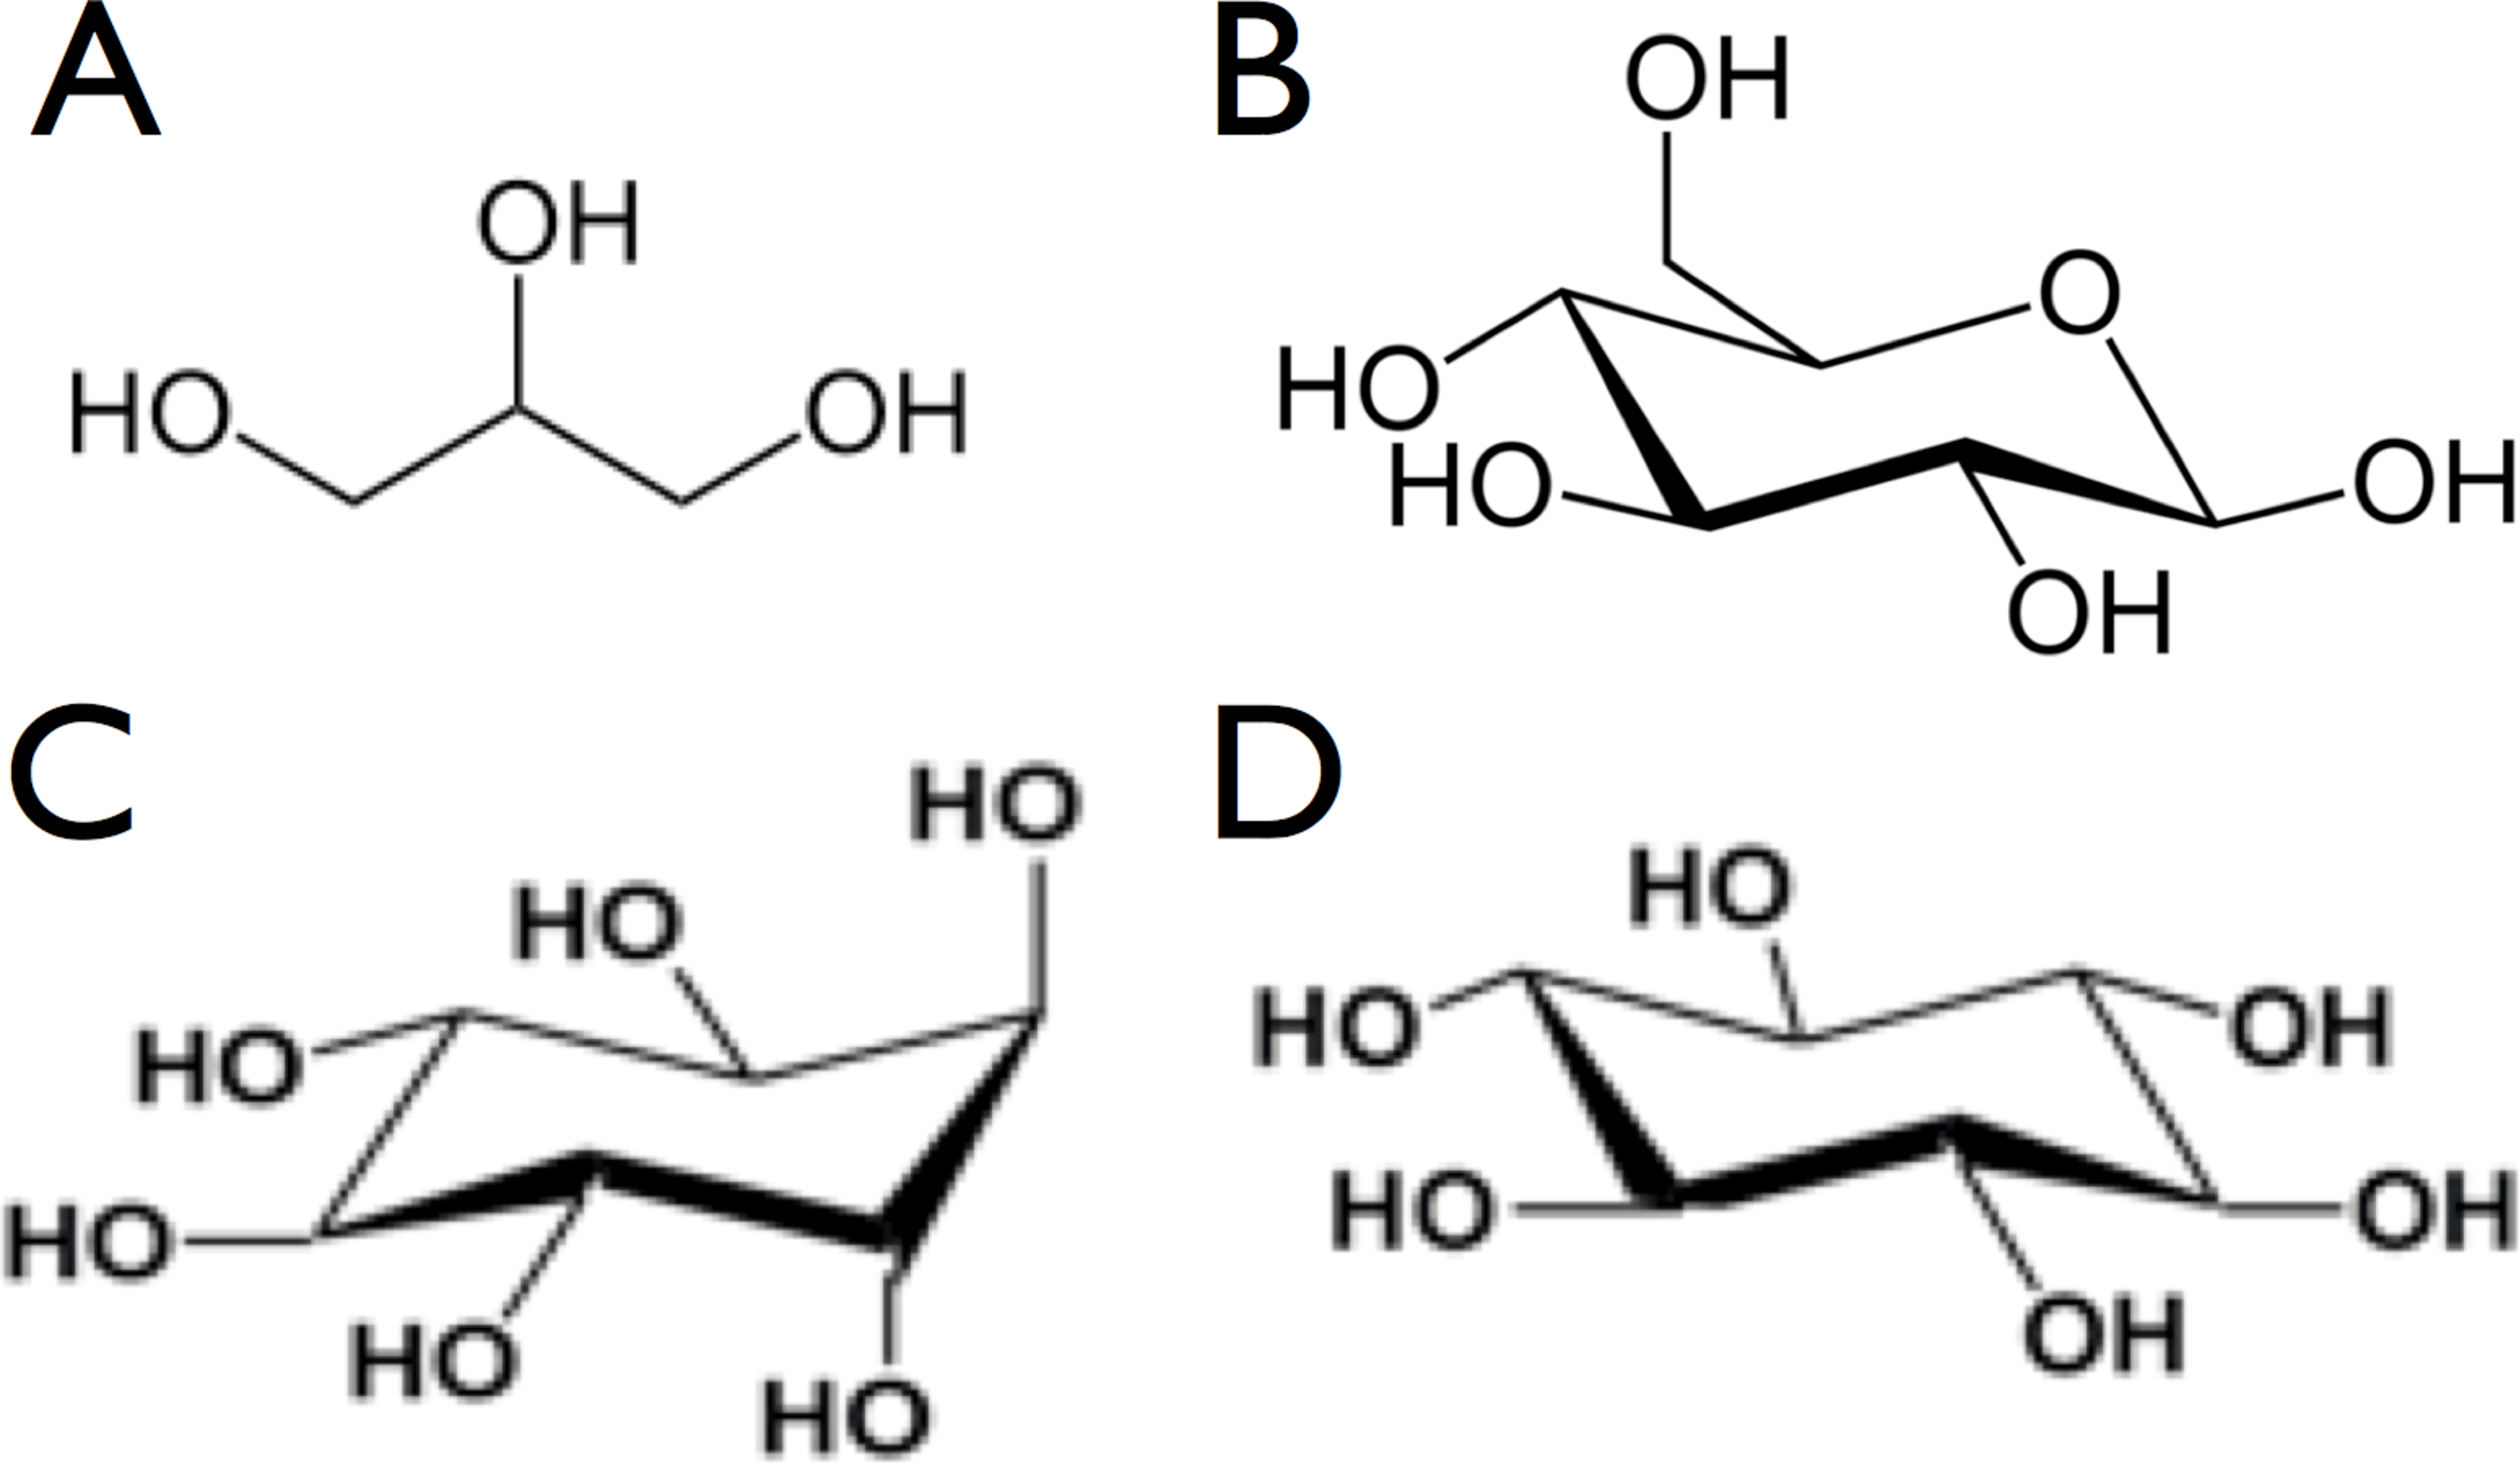
\includegraphics[width=2.5in]{figures/results3/ligands.pdf}
  \caption[Ligands]{Molecular structures of (A) glycerol, (B) glucose, (C) chiro-inositol and (D) scyllo-inositol}
  \label{fig:ligands}
\end{figure}

\begin{figure}[htbp]
  \centering
  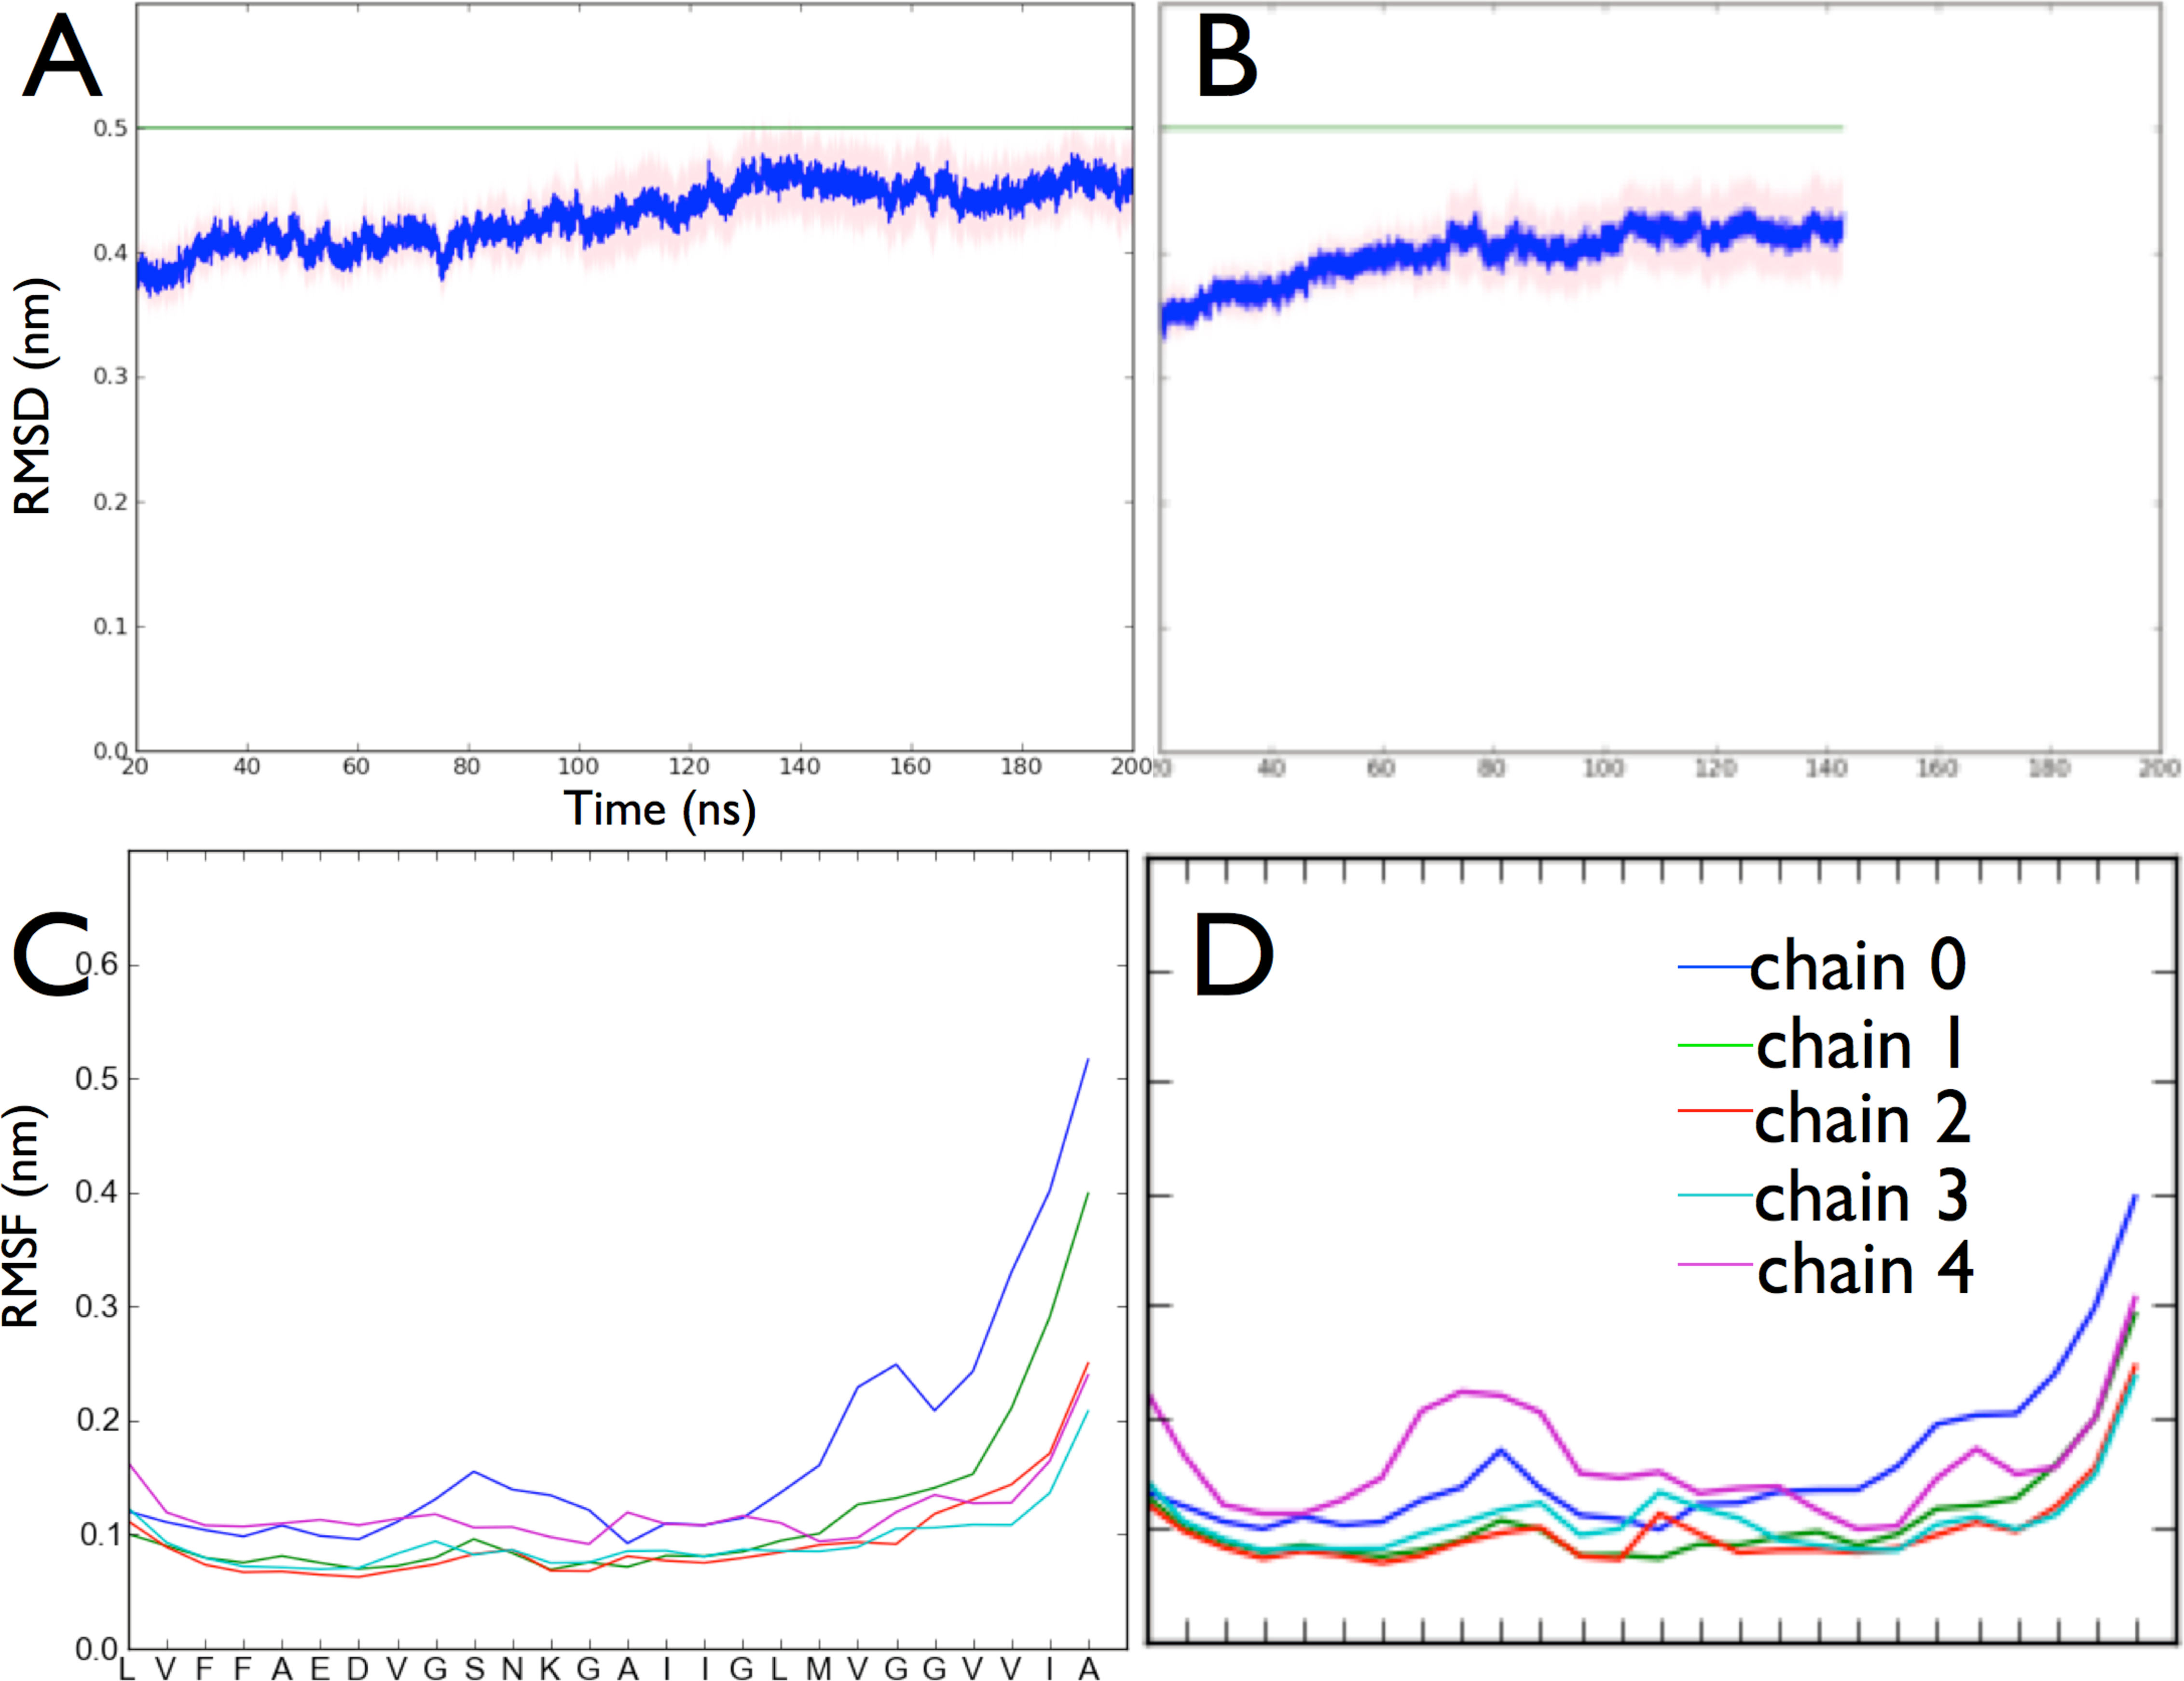
\includegraphics[width=5in]{figures/results3/protofibril_dynamics.pdf}
  \caption[RMSD and RMSF vs. time]{Fibril structure dynamics in pure water (A) and (C), and in the presence of scyllo-inositol (B) and (D).}
  \label{fig:protofibril_dynamics}
\end{figure}

\begin{figure}[htbp]
  \centering
  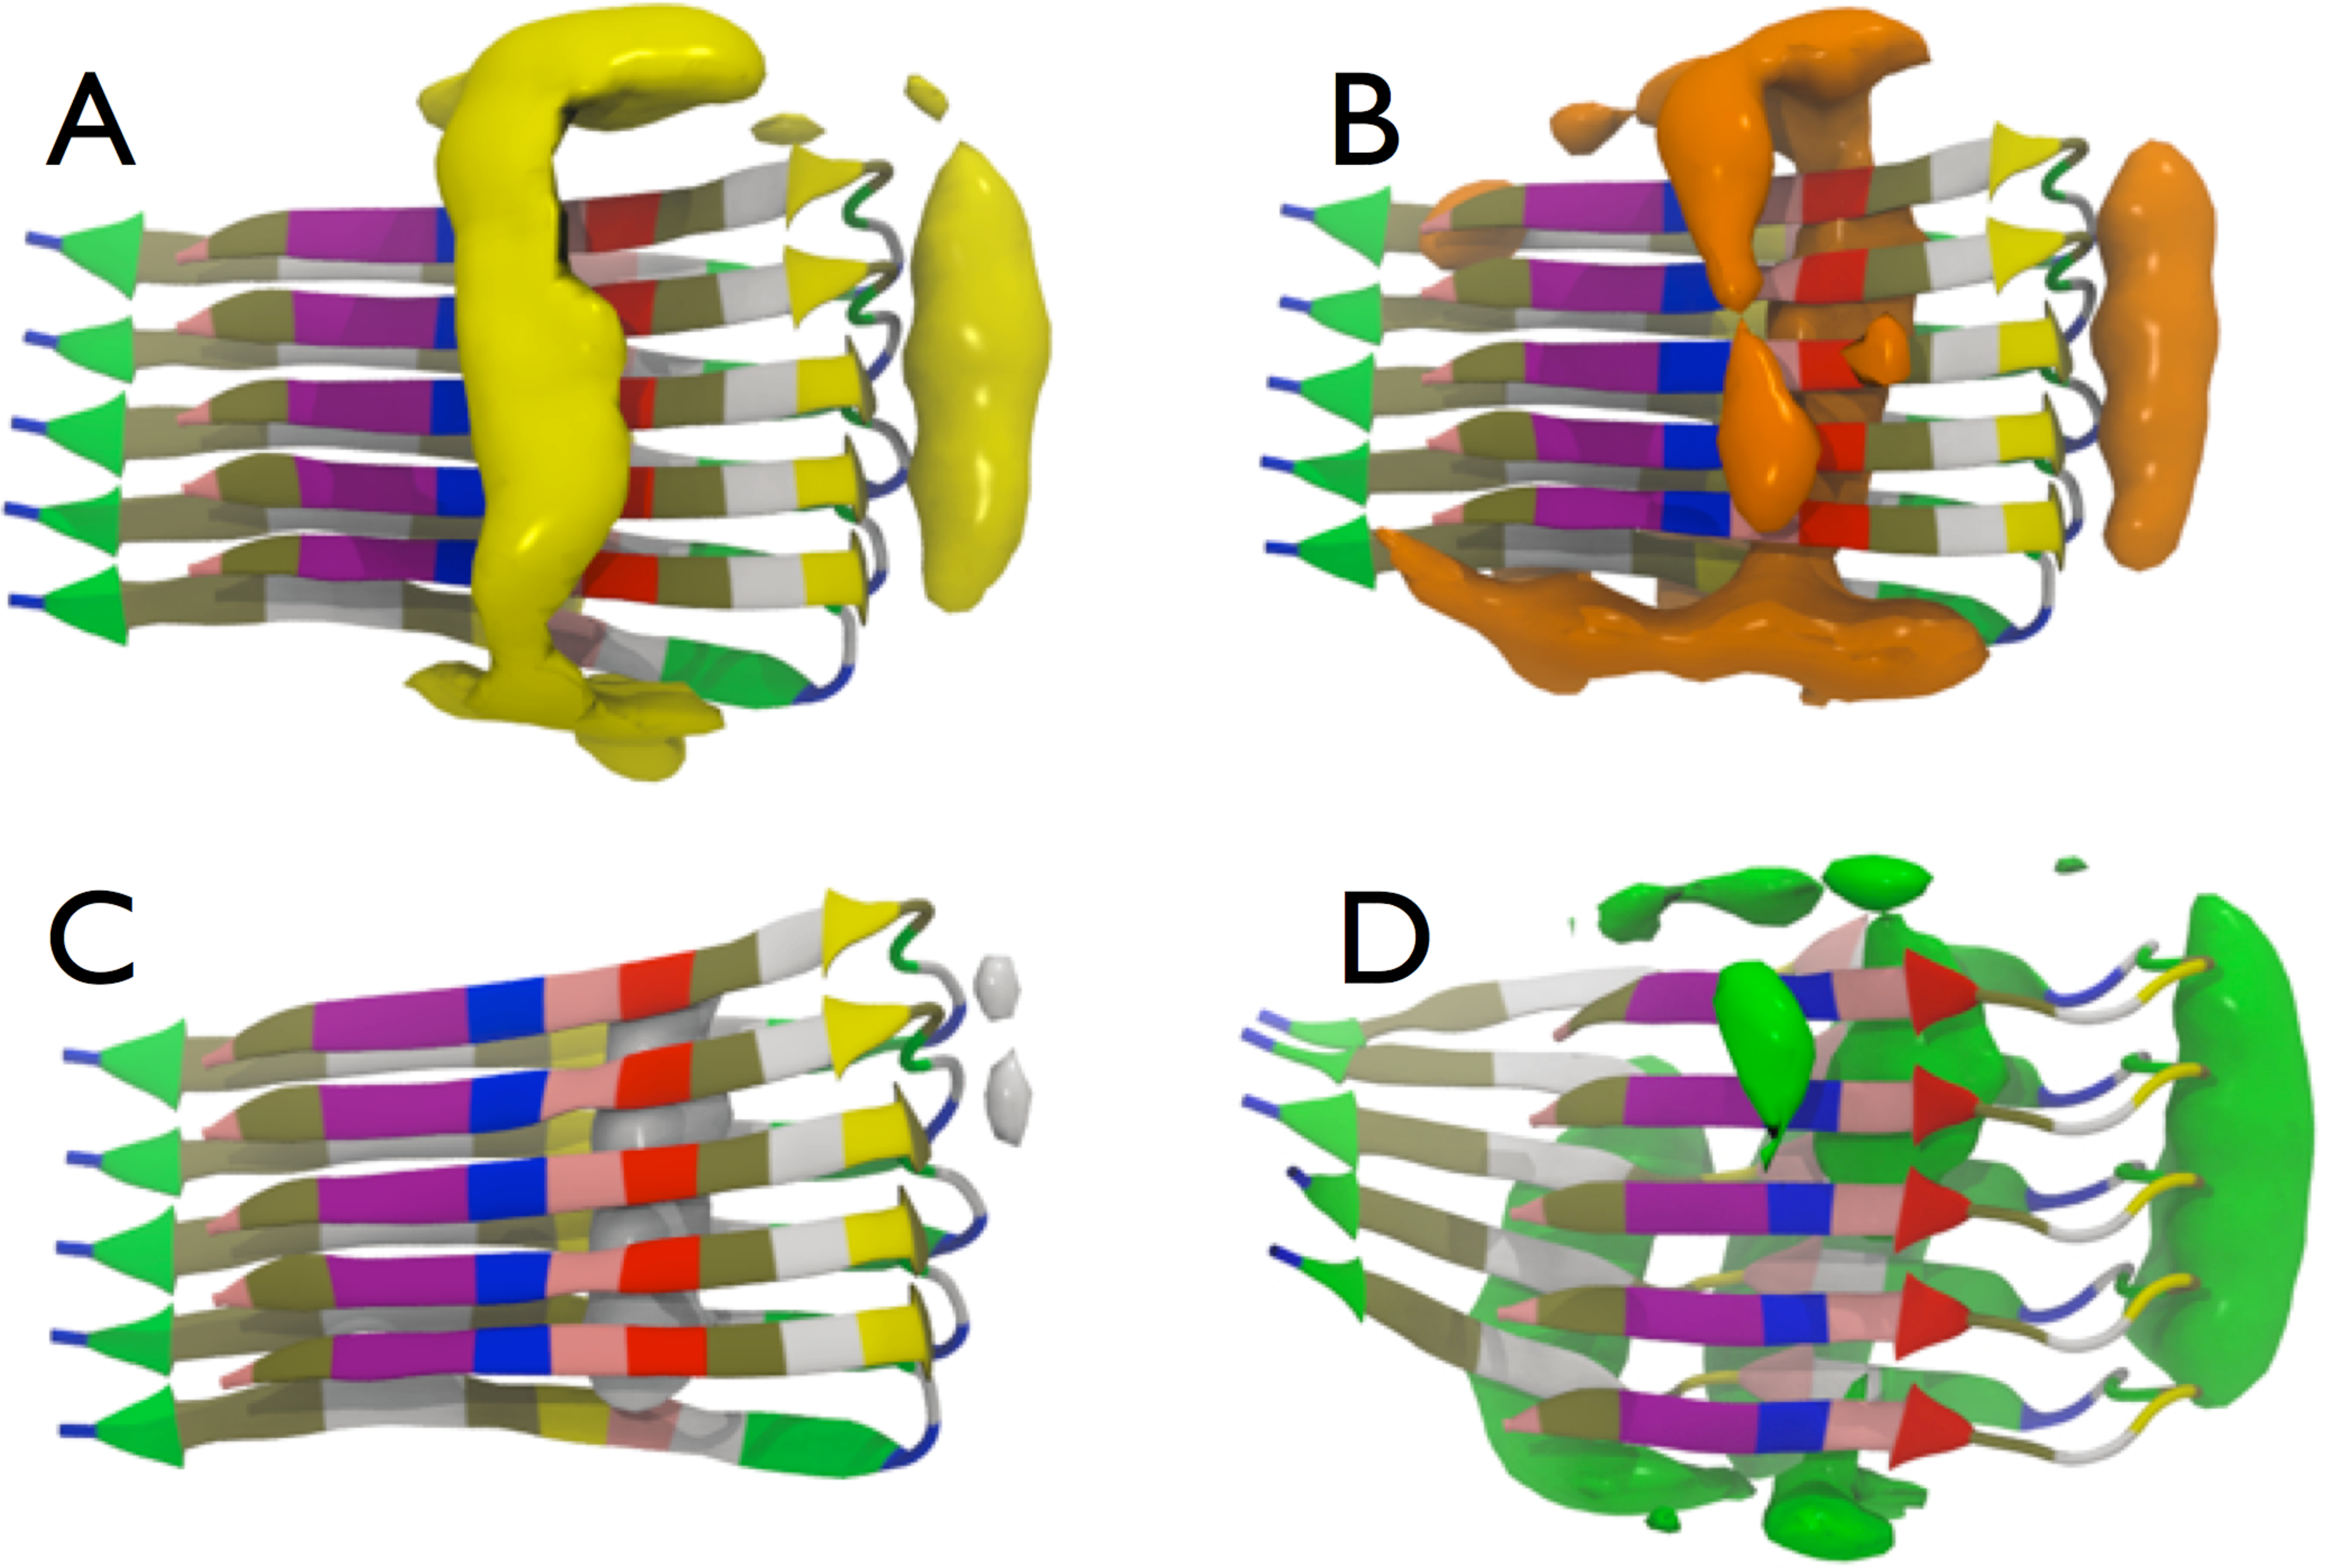
\includegraphics[width=6in]{figures/results3/binding_sdf.pdf}
  \caption[Abeta42 binding]{Comparisons of the spatial probability densities for (A) scyllo-inositol, (B) chiro-inositol (C) glycerol and (D) glucose.}
  \label{fig:spatial_binding}
\end{figure}

\begin{singlespace}
\addcontentsline{toc}{section}{Bibliography}
\bibliographystyle{elsart-num}
\bibliography{/Users/grace/github/thesis/document/results3/results3}
\end{singlespace}


 
% % PGab
%\author{Grace Li}
%\author{Christopher Ing}
% \author{Dustin Little}
% \author{P. Lynne Howell}
% \email{howell@sickkids.ca}
% \affiliation[University of Toronto, Biochemistry]
% {Department of Biochemistry, University of Toronto, 27 King's College Circle, Toronto, Ontario, Canada M5S 1A1}
% \alsoaffiliation[Hospital for Sick Children]
% {Molecular Structure and Function, The Hospital for Sick Children, 555 University Avenue, Toronto, Ontario, Canada M5G 1X8}
% 
% \author{Mark Nitz}
% \email{nitz@chem.utoronto.ca}
% \affiliation[University of Toronto, Chemistry]
% {Department of Chemistry, University of Toronto, 80 St. George Street, Toronto, Ontario, Canada M5S 3H6}

%\author{R\'{e}gis Pom\`{e}s}
%\email{pomes@sickkids.ca}
%\phone{416 813 5686}
%\fax{416 813 5022}
%\affiliation[University of Toronto, Biochemistry]
%{Department of Biochemistry, University of Toronto, 27 King's College Circle, Toronto, Ontario, Canada M5S 1A1}
%\alsoaffiliation[Hospital for Sick Children]
%{Molecular Structure and Function, The Hospital for Sick Children, 555 University Avenue, Toronto, Ontario, Canada M5G 1X8}

\chapter[MD simulations of PgaB-glucosamine binding]{Molecular Dynamics simulations of PgaB and monosaccharides of N-acetyl-glucosamine}
% The contents of this section were adapted from an article published in the \emph{Journal of Physical Chemistry}.

\emph{Reference}: Part of this work is published in ``PgaB Contains a Carbohydrate Binding Domain Required for Modification and Export of Poly-$\beta$-1,6-N-acetyl-D-glucosamine"
\\
\\
\emph{Contributions}:
Grace Li conducted the MD simulation part of the research and wrote the section. Dustin Little conducted and interpreted the experimental results. Chris Ing parameterized a key molecule for one of the simulations. Régis Pomès, Lynne Howell, Mark Nitz provided editorial input and guidance.

\newpage

\section{Summary}
% Note that this summary was taken from a draft of the paper written by Dustin from April 5th, 2013
Bacteria embedded in a self-produced matrix of exopolymeric substance, or biofilm, are tolerant to antibiotics, protected from the environment, and isolated from the innate immune system. Production and de-N-acetylation of the exopolysaccharide poly-$\beta$-1,6-N-acetyl-D-glucosamine (PNAG) is important for biofilm formation in Escherichia coli. PgaB is essential for the partial de-N-acetylation of PNAG (dPNAG); a process required for polymer export and subsequent biofilm formation. Here we report 1.9 Å crystal structures of PgaB’s isolated C-terminal domain (PgaB-CT) and complex with glucosamine. The structure of PgaB-CT has structural difference from the previously reported PgaB42-655 structure. Characterization of PgaB-CT using tryptophan fluorescence quenching assays shows binding to PNAG oligomers with ~1-4 mM affinity. These data in combination with molecular dynamics simulations of PgaB with N-acetylglucosamine and glucosamine suggest PNAG de-N-acetylation occurs first, with subsequent binding of dPNAG to the C-terminal domain. We believe this concerted action plays a pivotal role in targeting dPNAG for export through the outer membrane porin PgaA.

\section{Introduction}

% PgaB - description of the study, motivation and what has been done thus far
PgaB is a key protein that is responsible for the transport of the functionally relevant form of the exopolysaccharride poly-$\beta$-1,6-$N$-acetylglucosamine (PNAG), which is required for biofilm formation in a variety of bacterial systems. A crystal structure of PgaB was recently solved in the laboratory of Dr. Lynne Howell. Structural and functional characterization studies have shown that PgaB is composed of two domains, an N-terminal de-N-acetylase domain, and a C-terminal domain with structural homology to glycosyl hydrolases.\cite{Little:2012dp}
% PgaB structure has been deposited in the PDB -- I did not find this June 30th 2012

Currently, it is not known whether PgaB binds polymeric GlcNac or its de-N-acetylated end products, or both. Furthermore, binding modes, and lengths of putative substrate sugar polymers of PgaB are not known. Experimental characterization of sugar-bound structures of PgaB have been impeded by the insolubility of long sugar polymer chains (eg. those longer than a pentamer), and the weak binding of short sugar polymers (eg. di- and tri-saccharides). PgaB is hypothesized to bind sugar polymers (most likely a 15-mer) across its two domains at its surface. The polymer is speculated to extend out from the catalytic binding site (N-terminal domain) onto the charged grooves of the C-terminal domain.
% Experimentally it is known that shallow binding pockets exist at the surface of the proteins. REF?

Using molecular dynamics simulations, we exploit the weak binding affinities of N-acetyl-glucosamine (GlcNac) and glucosamine monosaccharides by using a fragment-based simulation approach to predict putative binding modes and sites of GlcNac and glucosamine. This methodology has been successfully applied in our previous simulation studies to examine the binding mechanism of inositol, a carbohydrate-like amyloid inhibitor, with amyloidogenic peptides and their aggregates. To our knowledge, this is the only study thus far in literature which employs large-scale MD simulations to predict sugar-protein interactions.

% The objective of my work is to predict PNAG binding sites at the surface of PgaB using unrestrained molecular dynamics simulations in the presence of GlcNac. This methodology was used in earlier inositol studies to predict inositol binding sites on amyloid peptides and aggregates.
\textbf{The directionality of the polymer binding.  This is currently not experimentally determined. Glucosamine molecules were observed in our simulations to form linear hydrogen bonded chains. When a vector is drawn from the X to Y atom of glucosamine, it is observed that each of the vectors have their NH3 groups facing the N terminal domain.}

% I don't fully understand the directionality business.  Here is a hack job at summarizing what it is from readings.
% From wikipedia -- An oligosaccharide has both a reducing and a non-reducing end. The reducing end of an oligosaccharide is the monosaccharide residue with hemiacetal functionality, thereby capable of reducing the Tollens’ reagent, while the non-reducing end is the monosaccharide residue in acetal form, thus incapable of reducing the Tollens’ reagent.[2] The reducing and non-reducing ends of an oligosaccharide are conventionally drawn with the reducing-end monosaccharide residue furthest to the right and the non-reducing (or terminal) end furthest to the left.[2]

% directionality paper
% http://www.jbc.org/content/274/37/26557.full
\section{Material and Methods}
% Modelling details
PgaB with a loop spanning residues 613 to 619 (numbered according to the chimeric PDB structure; check with Dustin again) in the N-terminal domain modelled into the truncated crystal structure, was used in our simulations. The initial crystal structure has Ni(II) bound at its enzymatic active site. Ni(II) is tetrahedrally coordinated with surrounding residues.  The acetate ion bound near the active site, an artifact of crystallization, was removed in the simulation. Crystal waters were removed from the initial PDB structure. Histidine protonation states were assigned based on predicted pKa values using the web software PROPKA (\url{http://propka.ki.ku.dk}), and histidine hydrogen-bonding geometries in the initial crystal structure.

Protein and ions were modelled using the AMBER99 force field.\cite{Cornell:1995td} Parameters for Ni(II) was approximated using the parameters for the magnesium ion (Mg$^{2+}$). After assigning protonation states of histidines, the net charge of the protein was -10e. The final simulation system comprised of 11 sodium (Na$^{+}$) counterions, and either 45 molecules of free $\beta$-N-acetyl-glucosamine (GlcNac) or glucosamine, at a concentration of 100 mM (Figure~\ref{fig:nag}). 19533 and 19991 water molecules were present in the GlcNac and glucosamine simulations, respectively. The initial volume of the simulation box is 713.6 nm$^{3}$.  To mimic experimental conditions, 100 mM of salt was added to the aqueous solution in glucosamine simulation systems.

% Note: To generate this structure from Glycam builder, choose the beta-pyranose ring and then acetyl-glucosamine
GlcNac molecules were generated using the web-based Glycam Biomolecule Builder (\url{http://glycam.ccrc.uga.edu/ccrc/biombuilder/biomb_index.jsp}). The GLYCAM06 force field for carbohydrates\cite{Kirschner:2008ii} was used to model GlcNac and glucosamine. A PDB of glucosamine-$\textrm{NH}_{3}^{+}$ was obtained from the ZINC database.\cite{Irwin:2005kx} Energy minimization was performed using the software GAUSSIAN-09.\cite{g09} The minimized glucosamine structure was consistent with the GLYCAM force field, and new RESP-derived partial atomic charges were computed for glucosamine (a net charge of -1e) by fitting to a single HF/6-31G* molecular electrostatic potential (MEP) with a restraint weight of 0.01. MEPs were computed using the CHELPG methodology\cite{Breneman:1990ue} with the R.E.D. III software package.\cite{Dupradeau:2010bb} The partial charges were assigned so that the HCNH3 group summed to a net charge of +1.164e, and the rest of the molecule summed to a net charge of -0.164e. Aliphatic hydrogen atoms were fitted with a zero partial charge in order to be compatible with GLYCAM06.
% How to cite the web builder - Carbohydrate Builder Woods Group. (2005-XXXX) GLYCAM Web. Complex Carbohydrate Research Center, University of Georgia, Athens, GA. (http://www.glycam.com) XXXX = current year

% Note put the partial charges used for glucosamine in an appendix. Ask Chris Ing to add to this methods description.  

The TIP3P water model was used to represent the solvent. Version 4.5.5 of the GROMACS software package\cite{Pronk:2013ef,Hess:2008p5353} was used to perform unrestrained all-atom MD simulations with the stochastic dynamics algorithm using an integration timestep of 2 femtoseconds.

% Better organize below to make clear that I was using different integrators for equilibration and production dynamics.
% I still need to remind myself what rcoulomb and rlist corresponds to physically in the MD algorithm
Electrostatic interactions were calculated using Particle Mesh Ewald (PME) summation with a grid size of 0.12 nm and a Coulombic real-space cutoff of 1.1 nm. The Lennard-Jone potential was computed up to 1.2 nm using the GROMACS twin-range cutoff function with a short-range cut-off of 1.1 nm. Covalent bonds involving hydrogens were constrained using the LINCS algorithm. The simulation system was first subjected to energy minimization followed by a 1 ns equilibration in the NVT ensemble using Berendsen temperature coupling at 300 K with a coupling constant of 2.0.

A second equilibration was performed for 1 ns in the NpT ensemble with isotropic pressure coupling. Temperature and pressure for equilibration were controlled at 300 K and at 1 atm, respectively, using Berendsen thermostat and pressure coupling schemes. Production simulations were performed using the stochastic dynamics (sd) integrator and the Parrinello-Rahman barostat for pressure coupling.
% Look at /mnt/scratch_mp2/pomes/ligrace1/pgab/protein_sugar/params for fill in the blank parameters here

\subsection{Analysis}
\emph{Spatial binding probability densities of GlcNac and glucosamine.} Frames from our simulations were first fitted to the initial starting state of the simulation (an MD equilibrated crystal structure) via RMSD alignment of the protein backbone atoms. The density map corresponds to the fractional atomic occupancy of GlcNac or glucosamine molecules in a grid with a resolution of 1 angstrom, accumulated over 900,000 time frames. The Visual Molecular Dynamics (VMD) software package was used to calculate and graphically render the densities depicted in Figures~\ref{fig:pgab_density} and \ref{fig:pgab_binding_sites}.
% By examining the structure - does the sugars arrange into predicted binding site (s)?


\section{Results and Discussion}

\subsection{Binding to PNAG}
Figure~\ref{fig:pgab_density} depicts the spatial binding probability density of bound GlcNac after a total of 1.8 $\mu$s of sampling from 13 independent simulations of a chimeric PgaB in the presence of 100 mM of GlcNac. In our coloring scheme, residue numbers 43 to 310 and numbers 311 to 667 represent N- (green) and C-terminal (cyan) domains, respectively. GlcNac binds on the surface of both domains of PgaB. Our simulations suggest that PgaB may be able to bind GlcNac. Binding is specific and is localized to three main sites on the protein (Figure~\ref{fig:pgab_binding_sites}). In particular, GlcNac predominantly binds in grooves located at the interface between the two domains, where many molecules are found to bind in clusters at the mouth of the N-terminal $\beta$-barrel, in close proximity to the active site.  Moreover, when overlapped with bound GlcNac molecules, the overall binding density map suggests that PNAG may be able to bind to PgaB by wrapping around the protein (Figure~\ref{fig:pgab_density}A and B).

While GlcNac molecules are able to bind on surfaces of both domains, qualitatively, they appear to preferentially bind to the C-terminal domain (Figure~\ref{fig:pgab_density}B and D). This is in corroboration with the fact that the C-terminal domain of PgaB is homologous to other carbohydrate binding domains (need to find REFs).

Moreover, our simulations have identified binding sites that were not able to be predicted by solely examining the static crystal structure. Binding densities suggest that the crevice found beneath the loop (residue numbers 309 to 314) which bridges the N- and C-terminal domains may be involved in sugar binding. The role of this region of the protein has not yet been determined experimentally. Significantly, our simulations correctly identified binding to tryptophan 613, a key conserved residue found in the C-terminal domain loop (residues numbers 613 to 619), which is known to bind carbohydrates in homologous proteins. Note that this loop was not resolved in the X-ray crystal structure and was modelled into the PDB structure for our simulations.

\subsection{Binding to NAG}

\textbf{The spatial distribution of NAG indicates that NAG preferentially binds the C-terminal domain of PgaB. Specifically, clusters of NAG molecules bind in the groove lined with acidic residues (Asp and Glu) (Figure~\ref{fig:pnag_nag_overlapped_zoomedout})}.  \textbf{In support of this preferential binding,  as depicted in Figure~\ref{fig:salt_density_distribution} salt ions do not significant bind the ion and are distributed uniformly over the protein.}

\begin{figure}
\centering
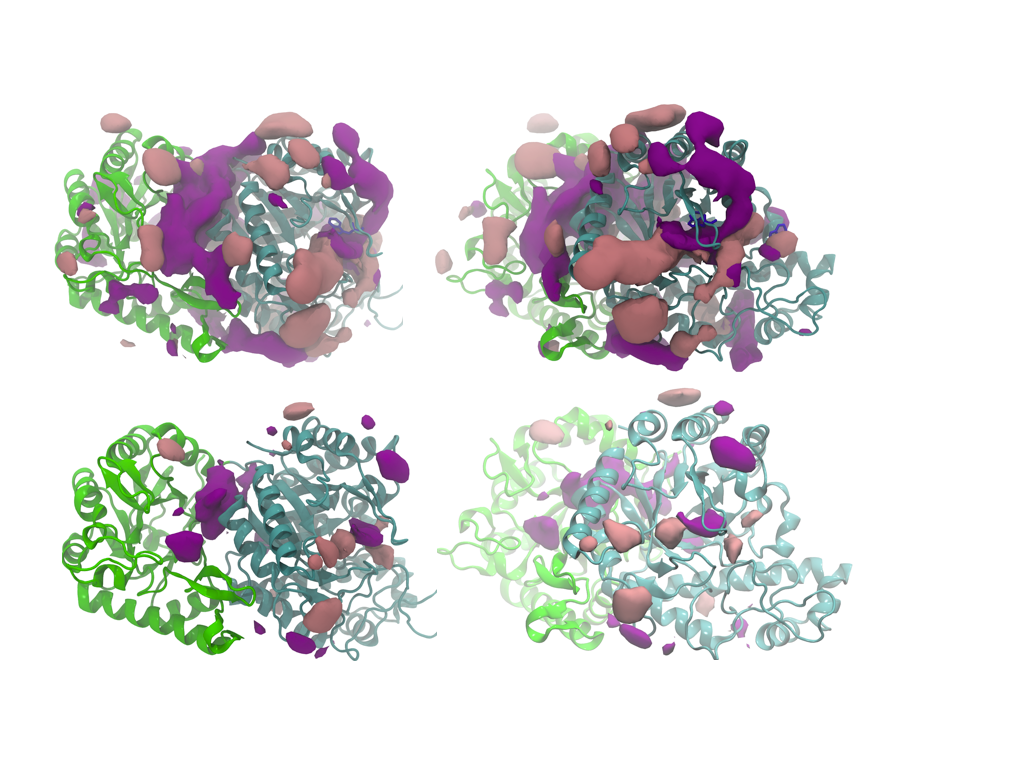
\includegraphics[height=4.1in, width=6.23in]{figures/results4/pnag_nag_sdf_zoomedout.png}
\caption{Comparisons of the distributions of bound PNAG and NAG.}
\label{fig:pnag_nag_overlapped_zoomedout}
\end{figure}

\begin{figure}
\centering
\includegraphics[height=4.1in, width=6.23in]{figures/results4/salt_distribution.png}
\caption[Ionic distribution]{\textbf{Not yet rendered}. Spatial probability distribution of salt ions around \pgab}
\label{fig:salt_density_distribution}
\end{figure}

\textbf{Furthermore, consistent with the crystal structure, in our simulations, glucosamine was observed to bind to tryptophan 613, adopting the exact binding mode shown by X-ray crystallography (Figure~\ref{fig:nag_cterminal_zoomedin}).}

\begin{figure}
\centering
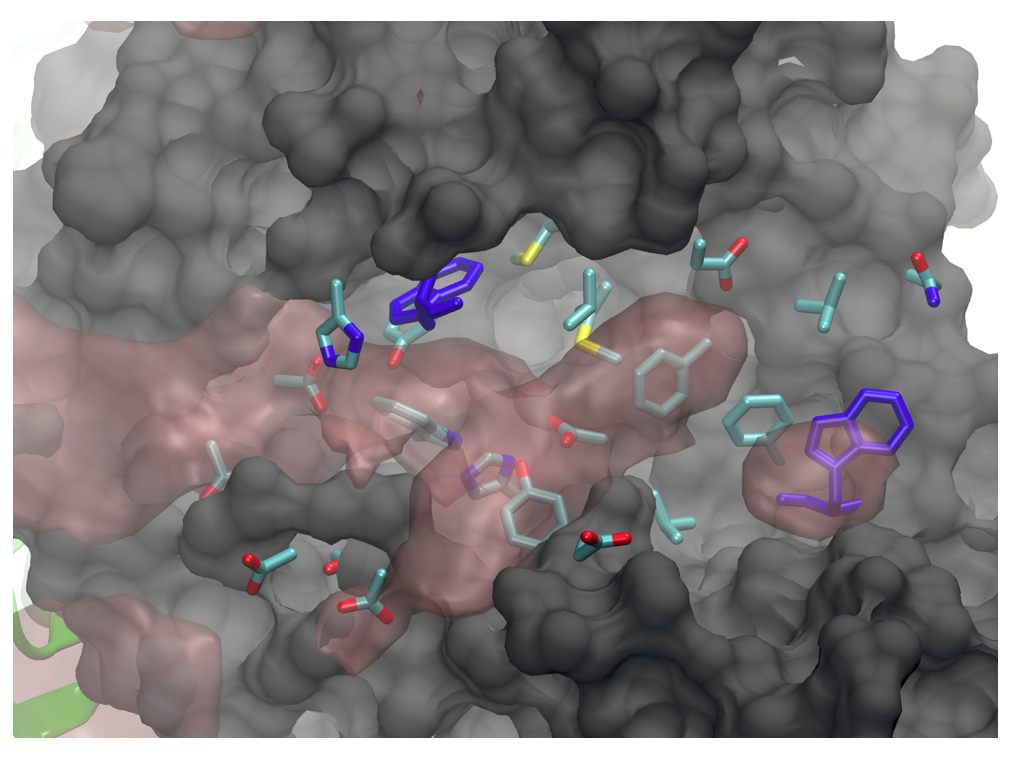
\includegraphics[height=4.1in, width=6.23in]{figures/results4/nag_cterminal_zoomedin.png}
\caption{Distribution of NAG in the binding groove in the C-terminal domain.}
\label{fig:nag_cterminal_zoomedin}
\end{figure}

% What is the name for positively charged glucosamine molecules? Is there a 3-letter abbrev. for it?
When comparing the densities of PNAG and glucosamine (depicted in Figures \ref{fig:pgab_density} and XXX, respectively) it can be seen that whereas PNAG predominantly binds the N-terminal domain, but glucosamine instead bind to the C-terminal domain, predominantly in the groove capped by the loop spanning residues XXX to YYY.  % Glucosamine is found to bind in the groove with acidic residues and aromatics.  Our simulation shows that glucosamine has a high affinity binding site at residue XXX. Importantly, this finding is consistent with X-ray crystal structures of full length pgab co-crystallized with glucosamine monosaccharides. Furthermore, glucosamine is predicted by our simulations to interact with residues X, Y, Z..., which are key conserved residues known to bind carbohydrates in other homologous carbohydrate-binding domains.

\section{Future Work}
In the future, it may be interesting to use a similar simulation approach to investigate the binding of glucosamine (GlcNH$_3^+$) monosaccharides and polysaccharides to PgaB.  Various analyses (eg. time evolution of RMSD, RMSF of the protein, principle component analysis, etc.) can be done to quantify protein dynamics, especially the mobility of the two domains. Furthermore, it will be interesting to investigate how dynamics may be correlated to the function of PgaB.  Finally, it will be interesting to predict GlcNac / GlcNH$_3^+$ binding modes and binding constants from MD simulations, and compare these predictions with corresponding future experimental results.

% This work is currently done in collaboration with Dustin Little, Dr. Lynne Howell and Dr. Mark Nitz.
% Run simulations with other monosaccharides such as glucosamine or glucose

% Binding surface - Map out a binding surface for both domains - We don't know what the C-Terminal domain is responsible for.  
%	- My simulation - suggests that it binds GlcNac?
% Compare and predict binding affinities.  Dustin is trying to get experimental data and co-crystal structures.

% \begin{itemize}
% 	\item Rmsd vs. time for the entire protein
% 	\item Rmsd vs. time for each of the individual domains
% 	\item Rmsf of the protein
% \end{itemize}


\begin{figure}[nag]
\centering
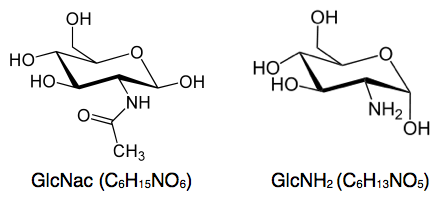
\includegraphics[height=1.5in, width=3in]{figures/results4/figure_pgab_sugars.png}
\caption[NAG]{$\beta$-N-acetyl-glucosamine (GlcNac) and glucosamine (GlcNH$_2$) monosaccharides.}
\label{fig:nag}
\end{figure}

\begin{figure}[pgab_density]
\centering
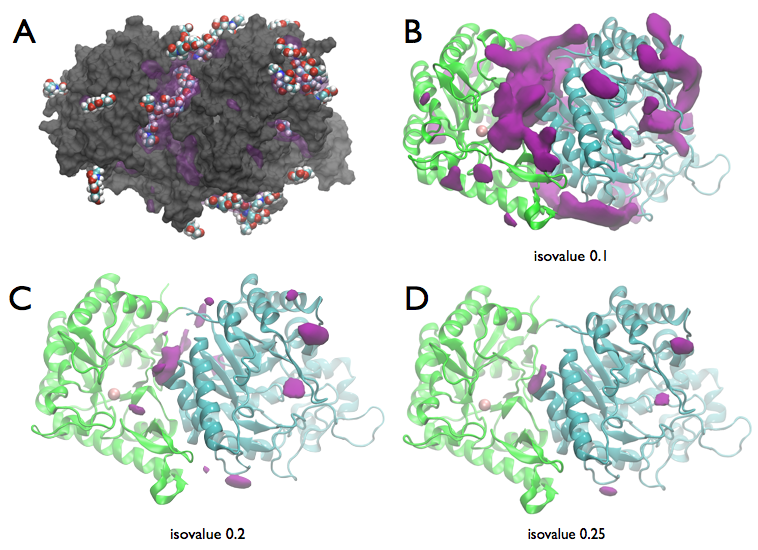
\includegraphics[height=4.25in, width=6in]{figures/results4/figure_pgab_density.png}
\caption[NAG binding density]{Spatial binding probability density map of bound GlcNac around PgaB. An example snapshot of PgaB (grey) shown using a surface representation (A) with bound GlcNac binding density  (purple) at iso-contour of 0.1 or 10\% occupancy. Binding densities of GlcNac overlapped with a cartoon representation of PgaB at iso-contour levels of (B) 0.1 (C) 0.2 (D) 0.25. N- and C-terminal domains are depicted in green and cyan colors respectively.}
\label{fig:pgab_density}
\end{figure}

\begin{figure}[pgab_binding_sites]
\centering
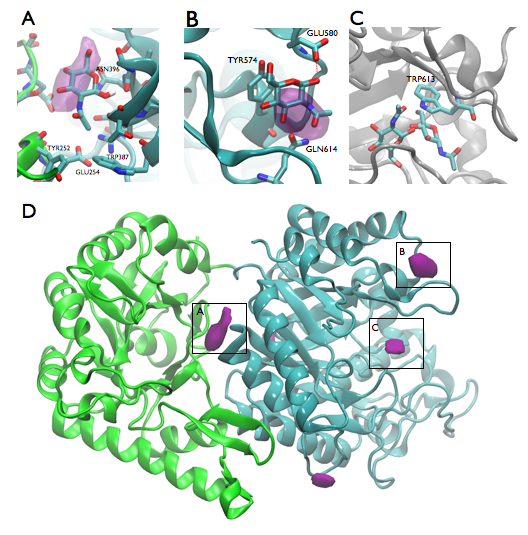
\includegraphics[height=6.29in, width=6.12in]{figures/results4/figure_pgab_binding_sites.png}
\caption[GlcNac binding sites]{High probability GlcNac binding sites at an iso-contour value of 0.25 (D). Insets (A to C) show detailed views of the binding sites and the residues involved in binding.}
\label{fig:pgab_binding_sites}
\end{figure}

\begin{singlespace}
\addcontentsline{toc}{section}{Bibliography}
\bibliographystyle{elsart-num}
\bibliography{/Users/grace/github/thesis/document/results4/results4}
\end{singlespace}

% Notably, our simulations were able to correctly predict binding to the tryptophan key to sugar binding.

% protein motion -- dynamics of the protein - can it be related to how it might function?

% NAG binding
% \begin{itemize}
	% \item Where does it binding? Highlight conserved residues on the protein.
	% \item Significantly, our simulations were able to identify binding to tryptophan 613, a key conserved residue in the XXX loop of the C-terminal domain which is involved in sugar binding. 
	% Dustin has a recent crystal structure showing a bound glucosamine TRPXXX, also a conserved residue.
	% \item Figure \ref{fig:pgab_density} shows the spatial probability density of bound NAG after a total of 1.8 $\mu$s of sampling from 13 independent simulations.  The density suggests that a bound PNAG may be able to wrap around the protein.
	% \item Snapshot of different binding densities at different iso-contour levels
% \end{itemize}

% Dustin has a recent crystal structure showing a bound glucosamine TRPXXX, also a conserved residue.


% % FIGURE
% \begin{figure}[pgab_rmsd]
% \centering
% 
\includegraphics[height=4.1in, width=6.23in]{figures/pgab_rmsd.jpg}
% \caption[PgaB protein dynamics]{Time evolution of RMSD of PgaB from its crystal state}
% \label{fig:pgab_rmsd}
% \end{figure}
% 
% % FIGURE
% \begin{figure}[pgab_rmsf]
% \centering
% 
\includegraphics[height=4.1in, width=6.23in]{figures/pgab_rmsf.jpg}
% \caption[PgaB protein dynamics]{Time evolution of RMSD of PgaB from its crystal state}
% \label{fig:pgab_rmsf}
% \end{figure}

% FIGURE
% \begin{figure}[pgab_domains]
% \centering
% 
\includegraphics[height=4.1in, width=6.23in]{figures/pgab_domains.jpg}
% \caption[PgaB protein dynamics]{Time evolution of RMSD of PgaB from its crystal state}
% \label{fig:pgab_domains}
% \end{figure}


% I guess i don't really know the extent of the anaylsis you can do (And by all means suggest options if i haven't touched on them in this email). At this point, it would be nice to know or map out a binding surface (for both domains). Because at this point - we still don't know what the CTerminal domain is responsible for, so your simulations could help suggest it binds GlcNAc. Also comparing relative binding constants would be very interesting as will, pending i can get experimental data such as binding data or co-crystal structures, to compare against. How difficult would it be to run the same simulations with glucosamine, or with a disaccharide modelled from GLYCAM? I don't really want to make too much work for you, just curious to know the effort that would take?

% At this point - i'm trying to get multiple co-crystal structures of the CTerminal domain, i was hoping i could see other spots where GlcNAc can bind - this would be neat to compare to your simulations if i can obtain more structures.
% 
% As for the binding data - i just started to do some tryptophan fluorescence with GlcNAc to see if i can obtain a binding curve. Ideally i would attempt this with GlcNAc and all the other saccharides up to the pentasaccharide. But there is the possibility it doesn't bind. well enough to obtain interpretable data. Keeping in mind, the protein acts on a big long polymer.
% 
% But to get back to your main idea - i'm blabbering on here, other then the density map and binding constants. I guess it would be nice to see where the most flexible parts of the protein are - and what this might correlate too. What other quantitative values can you obtain?
% 
% What program to you use to view your DX files - i can check if we have the on our suite of programs. If it is VMD then, yes we have it.

%%%% My reply %%%%
% Basically from our trajectories, I think I can reproduce things like
% B-factors, RMSD,  root mean square fluctuations, radial distribution
% functions etc ...  We have the full atomic structure along with the
% protein and the solvent dynamics.  We can definitely measure how
% dynamic the domains are by calculating the rmsf of the trajectories
% around the average protein structure in our trajectories to get a
% qualitative idea of where the most mobile region is. We can also do
% more advanced analysis of the protein domain motion, but I'm probably
% not going to have time to do this, but perhaps someone else in my lab
% can do this.  We can also look at the hydration of the binding site,
% coordination of residues, metal ions at the binding site (may not be
% entirely accurate), etc ...
% 
% I think the most interesting part is being able to compare and match
% it up to your experiments.  I think this will result in the most
% impactful second publication.  Perhaps I won't be the one to write the
% final paper, but if I do some of these analyses now, my hope is that
% it will inspire new hypothesis for you (or Mark) or add to the
% emerging story of the mechanism of PgaB.



 
% % Discussion / Perspectives
%\chapter{Perspectives, Conclusions and Future Directions}
% Example sentences found in teh conclusions and summary chapters of people's thesis 
% The work presented in this thesis has ...

% Because this work represents the first atomistic simulation, to our knowledge, demonstrating that polypeptide chains can form entangled polymer melt-like states, it contributes to an improved understanding of both elastin coacervation, and the more general phenomenon of protein aggregation

% Everyone's conclusions all had a significant amount of Future directions. (~3 pages worth)
% Strategy:  take the conclusion paragraphs of each chapter and then meld it into a conclusions chapter.

% Make a clear and concise statement of the original contribution to knowledge found in your thesis.

%What has this work led to?
%This has led to the understanding of mechanism of amyloid formation.
%An exploration of carbohydrate binding.


% One sentence summarizing AD and the medical challenges that it poses.  Summarize why it is difficult to design a drug for AD. 
% Summary of the core technique that is used in this thesis
Alzheimer?s Disease (AD) is a devastating neurodegenerative disease that is the most common cause of dementia in persons of age 65 or older. Currently there is no cure or method of treatment that targets the underlying disease.  As the world's population is living ages, AD will reach epidemic levels and will pose a tremendous medical burden for society. The overall goal of this thesis work is to investigate the molecular basis of amyloid inhibition by inositol, a small-molecule putative therapeutic for the treatment of Alzheimer's disease. By utilizing molecular dynamics simulations, a computational technique based on classical physics which allows us to simulate the motions of physical systems at the atomistic-level, we systematically examine model amyloidogenic peptides and aggregates to more complex systems involving the full-length A$\beta$42 peptide. The work presented in this thesis contributed to 2 peer-reviewed articles and 2 manuscripts in preparation which form the basis of Chapters 3 to 6.  The key results from each of these chapters are summarized below.

Beginning in chapter 2, I performed systematic simulations of simple amyloidogenic peptide models with scyllo- and chiro-inositol, stereoisomers of inositol, to examine the role of backbone binding on amyloid inhibition. My results indicated that although peptide backbone dominates the interaction with inositol, the binding affinity is low and remains in the millimolar range. Moreover, this property is independent of stereochemistry and does not appear to be sufficient to impede peptide dimerization through intermolecular backbone hydrogen bonding. Taken together, my results in this chapter suggest that amyloid inhibition by inositol cannot be accounted for by generic binding to the peptidic backbone alone. Rather, it is likely to involve sequence-specific interactions with amino-acid side chains as well as binding to specific aggregate morphologies.
% Accordingly, although the formation of intermolecular hydrogen bonds is the predominant interaction in protein aggregates composed of \gafour, amyloidogenic peptides involved in amyloid diseases are often more hydrophobic and in general, self-aggregation is driven largely by the hydrophobic effect.\cite{Chiti:2006p20}

To further investigate the role of sequence-specific interactions between inositol and aggregates of pathogenic peptides, I examined the binding of  inositol stereoisomers, successively to monomers, disordered oligomers, and $\beta$-sheet aggregates of A$\beta$(16-22), whose sequence is thought to be the core aggregation region in the A$\beta$42 peptide (chapter 4). A key finding of this study was that the $K_{eq}$ of inositol ($\sim$0.2 - 0.5 mM) for the $\beta$-oligomer is commensurate with the concentration at which inhibition of amyloid formation by A$\beta$42 is observed \emph{in vitro}. Although both \emph{scyllo}- and \emph{chiro}-inositol exhibit similar binding affinities with all peptide states considered, my simulations have uncovered a stereospecific face-to-face stacking stacking mode of \emph{scyllo}-inositol with the Phe side chains and a higher propensity for hydrogen bonding, which together suggests a molecular basis for measured differences in activity. \textbf{Cooperative binding modes of inositol at grooves on the surface of the $\beta$-oligomer of A$\beta$(16-22) suggest a possible mechanism of fibril inhibition whereby inositol prevents the lateral association or stacking of protofibrillar $\beta$-sheet oligomers.} Furthermore, my results suggest that the fibril core of A$\beta$ amyloid aggregates contains carbohydrate-like binding sites.  \textbf{As such, carbohydrate-based small-molecule derivatives may be a promising avenue to explore for the rational design of novel therapeutics for AD.}

In chapter 4, I investigate the binding of inositol to the protofibrillar form of A$\beta$42, the full-length peptide. Here, I found that there were no differences in the fibril conformations with and without inositol in either low or high molar ratio. 
% Does glucose bind more or less? If it does bind less, then it tells us that we might be onto something with scyllo-inositol even though the structure is subtly different.  
% Not sure what I meant here
Glucose does not necessarily bind ``less", but it does not bind on the right face ie. the KLVFFAE face Scyllo-inositol appears to preferentially bind the KLVFFAE face, more than glucose and chiro-inositol.  Furthermore, scyllo-inositol does not bind in a hydrated tunnel formed in the protofibrillar aggregate, where as both chiro-inositol and glucose Binding mode differences between active and inactive inhibitors of Abeta suggest a mechanism of inhibition.

In chapter 5, I demonstrated the generality of the methodology that was developed to study the binding mechanism of inositol by using a similar approach to study carbohydrate-protein binding. Specifically, ....  

\section{Significance for drug development for AD}
%[Thesis significance - part of the summary of what I make of my thesis ] 

There are a multitude of challenges in understanding the mechanism of a drug for treating neurodegeneration

This thesis demonstrates the applicability of MD simulations in providing insight into how drugs might bind to amyloidogenic species and intrinsically disordered peptides.  The results in this thesis can be used to map out a pharmacophore for developing a drug for the treatment of Alzheimer's Disease, opening the way to computer-aided design of improved diagnostics and therapeutics. A pharmacophore is an abstract description of molecular features which are necessary for molecular recognition of a ligand by a biological macromolecule - If I have to define this here, then it should have been in the introduction. \textbf{Definition is taken from the wiki.}

% Speculate on the future of drug development for AD in regards to the significance of thesis wrt curing AD. Will blocking aggregation work for AD? - May be this should in the introduction instead.
% (WRITE SOME CONCLUSIONS HERE … RELATING TO HOW A SINGLE SMALL MOLECULE BINDS SPECIFIC MORPHOLOGICAL STRUCTURES -- clearly a key result of my works demonstrate that there is sequence specificity) 

Because AD may be caused by a multitude of pathological changes in the brain, it is likely that a cocktail of compounds, each targeting a different disease pathway, may be required for treating AD. % (Adapted from pharmacophore for AD 2011)

% \section{MD simulations and Rational drug design}
\section{Contribution to sugar-protein binding}
% MD simulation as a tool for probing weak interactions
The work presented in this thesis have demonstrated that the methodology used in this thesis may be generally applicable to understanding carbohydrate-protein interactions. In chapter 4, we used simple sugars glucosamine and GlcNAc to map out a binding surface on PgaB, a protein invovled in the biofilm formation pathway. 

My work has demonstrated that MD simulations in combination with the use of current force fields can be effectively used to probe weak and transient molecular interactions, which are often not readily detectable using experimental techniques. One prominent example where weak interactions are prominent in protein-ligand binding is protein-carbohydrate interactions.\cite{weak binding review paper}

Understanding protein-sugar interactions is an important endeavor because of antibody binding to proteins.  Viruses often express carbohydrates on their coats.  Inhibiting bacterial action involves knowing how polysaccharrides are expressed, which involves binding proteins.  The results of this thesis presents methods that may be useful for developing antibiotics. \textbf{Rewrite this part to reflect and tie into how my work, methods, and how they are related to solving these problems} 

% The role of simulations in drug discovery to effectively predict binding modes and binding sites

[Thesis significance; more perspectives] Traditionally computation studies probing protein-ligand binding is often carried out with the knowledge of a putative binding site (often determined by X-ray crystallography) and the mechanism is examined employing sophisticated methods using the ligands thought to be able to bind in this specific pocket, while ignoring all other possibilities.  However, with the computing power to extend simulations to a longer time scale, MD simulations may be accurate in discovering new binding sites (even sites that are XXX high in affinity) without prior assumptions about the binding site. Our studies are among those which demonstrate the utility of MD to probe for binding sites that are difficult to obtain via experimental structural determination methods.  A recent MD study have demonstrated the capability of MD in binding site prediction for a folded protein.\cite{Shan:2011bo}

% Shan, 2011 (the DE shaw letter) An emerging challenge in drug discovery concerns the identification of allosteric ligand-binding sites (I’m not entirely convinced yet that this is important -- because I can’t think of any situations where this might be important -- convince myself or just drop this idea), through which drugs can modulate the effects of ligands that bind at the primary site.  More generally, an important limitation of traditional virtual drug screening is that it must start with a well-defined binding site (look into limitations of current drug discovery processes … may give some clue for constructing an argument for how MD is helping …), despite promising recent developments.\cite{Hetenyi, C.; van der Spoel, D. FEBS Lett. 2006, 580, 1447. (11) Davis,I.W.;Raha,K.;Head,M.S.;Baker,D.ProteinSci.2009, 18, 1998. }

\section{Significance for disordered binding}
% [Conclusions - A general interest in the specific work that I have done here ] 
Aside from contributing to the design of future AD therapeutics, our results have also contributed to the understanding of small molecule binding to disordered peptides (IDPs) in general. This is important because disordered binding are ubiquitous in biology, and disordered peptides and proteins and involved in many diseases such as X, Y, Z.  

Understanding how small molecules may interact with intrinsically disordered proteins goes beyond amyloid-related disorders. As IDPs are involved in many signalling pathways, they are also viable drug targets for many diseases.   Hence, targeting these disordered peptides using small molecules may be a possible therapeutic approach. For example, c-Myc is frequently involved in many cancers, \textbf{FILL IN THE GAP ABOUT HOW IT WORKS} and thus disruption of the c-Myc–-Max interaction is a possible anticancer strategy.\cite{Iakoucheva:2002uv,Metallo:2010p6822,Cuchillo:2012bm}

The work presented in chapters in this thesis sheds light on the mechanism of binding disordered peptides, and represents a step forward in understanding how small molecules may prevent protein - protein interactions, which involves identifying the binding interfaces, and understanding how to target these interfaces using small molecules.REFs.

\section{Osmolyte effects, denaturation, and macromolecular crowding}
% Note this is another hairy field … and you might want to stay the hell away from it, despite the fact that your thesis is loosely connected to this field
Another field of interest where weak interactions dominate is cosolvent effects on peptide folding. Simulations are a good use for probing that.  For example, MD simulations have been useful in gaining insight into protein denaturation mechanisms by urea or guanidinium, and the activity of osmolytes. Many of these are still open questions.\cite{http://pubs.acs.org/doi/abs/10.1021/jp200625k -- crowding and protein association.} Where am I going with this?

% These ideas below are  lesser developed ideas … consider cutting or bulk up …
% \section{other areas that are related to my work}
% [Ab-GAG membrane binding] This branches off the fact that I looked at sugar binding with peptides - amyloids when deposited may interact with glycosaminoglycans (part of the extracellular matrix) exposed at cellular surfaces. So what about it? Is my work helping to understand how amyloids are interacting with GAGs? or what role GAGs might play in accelerating amyloid formation?


% \subsection{Relationship to Polypharmacology -- where one drug binds to different targets?}
% Not sure how my thesis relates to this.

% I think this section is too crazy - eliminate.
%\section{In the future - perspectives on computer simulations}
% TODO: Find out why are there so few new drugs being discovered nowadays?
% Expand simulations into the macroscopic level 

% TODO: A good thought experiment - If I had the perfect simulation system? Predictive force field, simulate milliseconds in days.  How could I use this simulation system? Some effective use of the data? 

%Software has the ability to revolutionize drug discovery and take it from bench to personalized medicine. Molecular simulations can play a role in driving experimentation by helping to generate testable hypotheses.
%
%Virtual drug screening method using MD simulations as a component predicting drug toxicity.
%
%Here I'm speculating what the future of MD simulations might be ... A bit like science fiction with a touch of reality.
%
%Most Useful to “somehow” integrate experimental data with simulations results\cite{that nature paper discussing integrating MD and systems biology}
%- What are some success stories?
%what’s the real problem with drugs?
%Can we do without drugs? What are the therapies available?
%Small molecule
%peptide
%antibodies
%gene therapy (viral)
%\cite{Hansen:2012hh}

\section{Future directions}
% Better methods? Longer simulation times? Better force fields to detect hydrophobic effect?
% Better understanding of the amyloid aggregation mechanism will lead to a better understanding of the inhibition mechanism.

These are significance points.  Tie them better Studying different aggregate forms is useful.  One major conclusion of this thesis is that doing comparative systematic simulations is needed and useful for understanding the molecular basis of amyloid inhibitors how work.
[sketchy and would require a fast compute cycle -- look into more literature to formulate this idea better] This thesis shows that MD may be useful in the rational design of amyloid inhibitors from a template inhibitor. Molecular information obtained from simulations can be used to help design new derivatives, and simulations can be run for these chemically-modified forms of derivatives. 

\subsection{Simulations for other peptides involved in amyloid disorders}
Hard disk space and cpu power can be easily secured.  It would be a minor point to get that done.  Since there are many amyloid-associated disorders. In the future, simulations can be performed with these peptides while using a similar methodology. 

\subsection{Effect of inositol in the presence of lipid membranes}
Effect of the drug in the presence of lipid membranes => How does it affect aggregation in the presence of membranes. Does it prevent peptides from binding to the membrane?

\subsection{Apply enhanced sampling methods to study amyloid inhibition}
Extend simulations. The goal is to be able to simulate the entire aggregating process.  But this is not feasible because the timescale of fibril formation can take up to days. But can simulate the early stages of amyloid formation.  Use of enhanced sampling methods for aggregates in the presence of the drug.  These methods can enhanced Replica-exchange.  These methods enhance sampling and can speed up beta-sheet formation. With longer simulation times, can reach beta-sheet formation for shorter peptides such as KLVFFAE, we can add inositol (or some other drug) to understand their activity in early amyloid formation.


\section{Limitations}
Length of the peptides

\textbf{Lack of experimental data.} Finally, it would important to combine simulations with experimental studies.  This is a deficiency of this study. Simulations can be a good tool when combined with experimental validation by using a variety of techniques SSNMR and other biophysical techniques used to probe amyloid systems. Several studies are beginning to do that to understand the molecular mechanism of small molecule inhibitors ECGC.  In recent years several studies have begun to do this with some successes.




\end{document}
